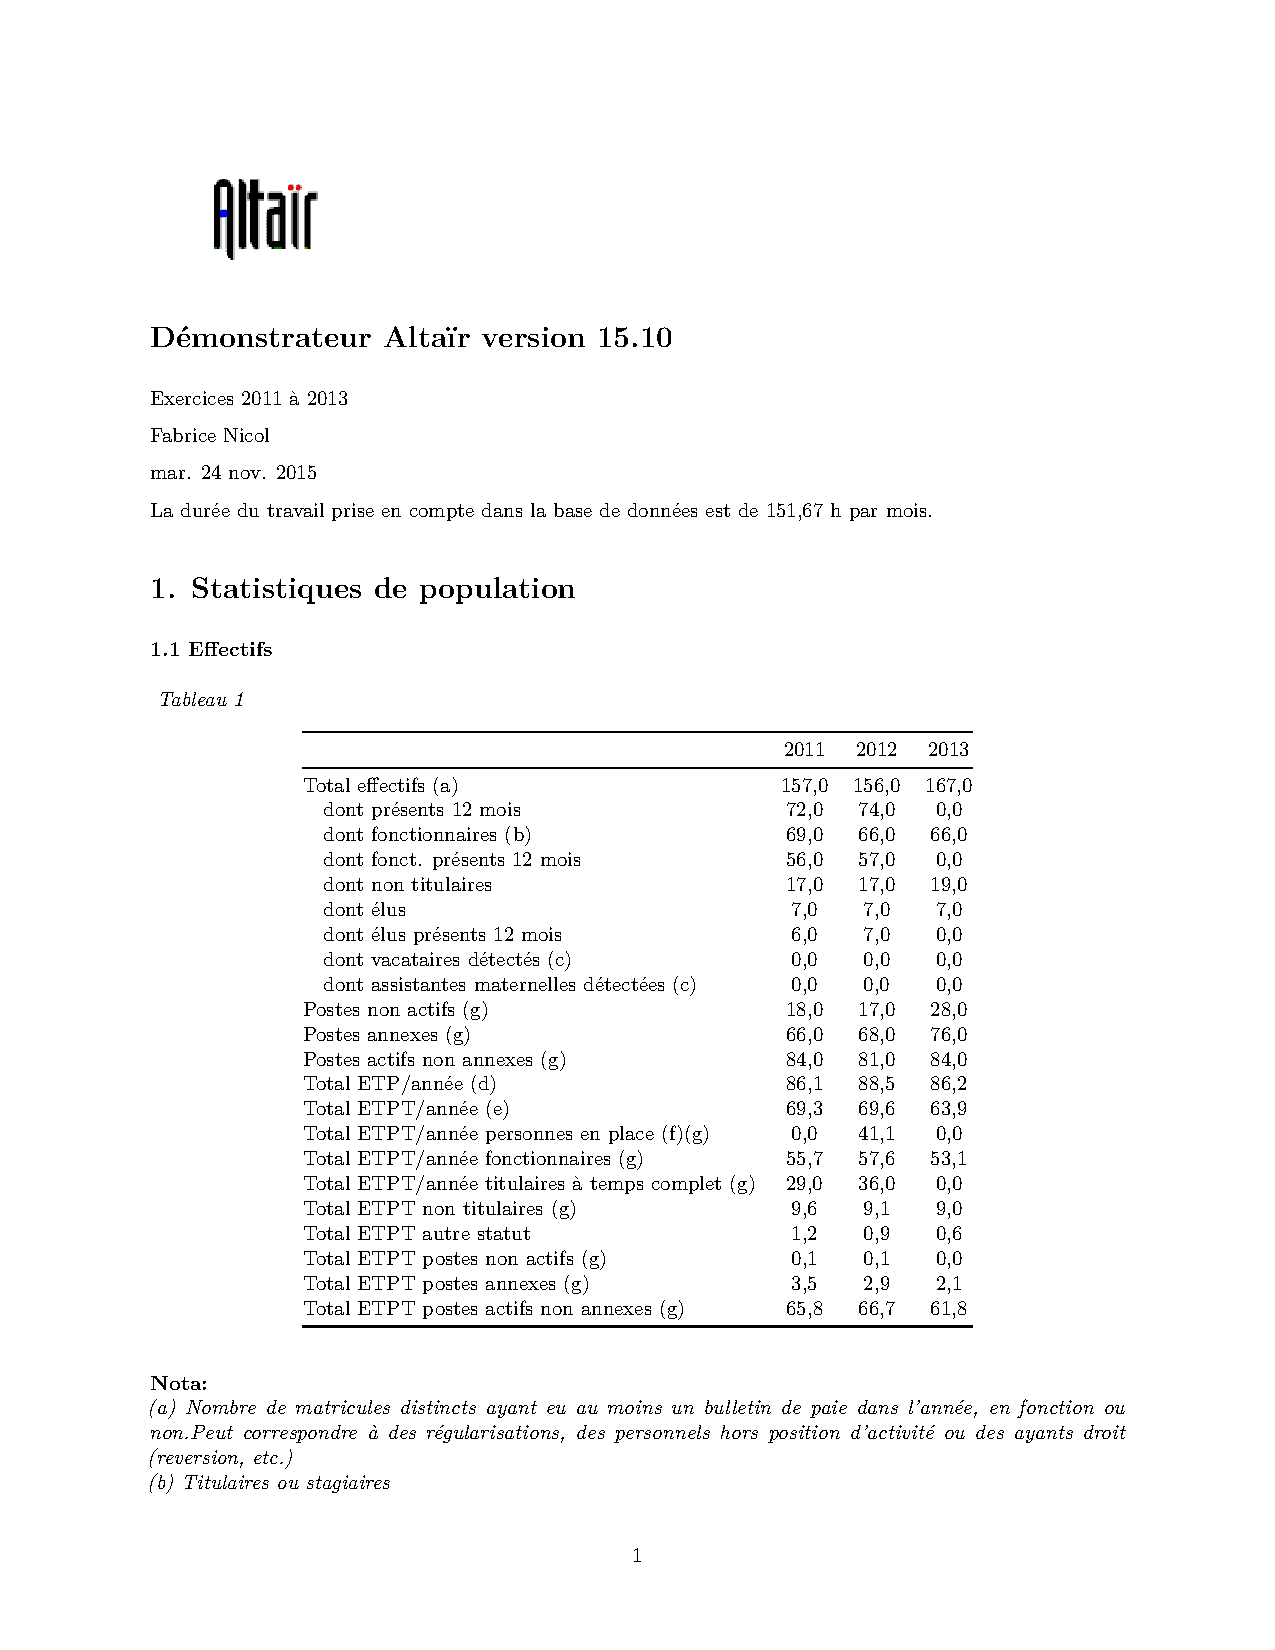
\includegraphics{icones/altair.png}

\hypertarget{logiciel-altair-version-20.08-4}{%
\subsection{Logiciel Altaïr version
20.08-4}\label{logiciel-altair-version-20.08-4}}

\hypertarget{employeur-yyy}{%
\subsubsection{Employeur : YYY}\label{employeur-yyy}}

\hypertarget{siret-yyy}{%
\subsubsection{Siret : YYY}\label{siret-yyy}}

\hypertarget{etablissement-yyy}{%
\subsubsection{Etablissement : YYY}\label{etablissement-yyy}}

\hypertarget{budget-budget-principal-assainissement-multi-budgets}{%
\subsubsection{Budget : BUDGET PRINCIPAL, ASSAINISSEMENT, Multi
budgets}\label{budget-budget-principal-assainissement-multi-budgets}}

\textbf{Période sous revue : 2008 - 2012 }\\
\textbf{Nombre d'exercices : 5 }

Logiciel sous licence \href{../Docs/LICENCE.html}{CeCILL v.2.1}

ven. 14 août 2020

\textbf{Avertissements}

\emph{1. La production des rapports d'analyse nécessite que les données
de paye soient continues, autrement dit qu'il n'y ait pas d'année ou de
mois manquant dans la série de données disponibles. Lorsque tel est le
cas, il convient de réaliser autant de rapports partiels que de séries
partielles de données continues.}

\emph{2. Il est recommandé de renseigner, dans toute la mesure du
possible, les codes de paye de l'onglet Codes de l'interface graphique}
~
\href{../Docs/Notices/fiche_onglet_codes.odt}{\includegraphics{icones/Notice.png}}

En cas de dysfonctionnement logiciel, veuillez bien signaler les
difficultés rencontrées au développeur.

\hypertarget{statistiques-de-population}{%
\section{1. Statistiques de
population}\label{statistiques-de-population}}

\hypertarget{effectifs}{%
\subsection{1.1 Effectifs}\label{effectifs}}

~\emph{Tableau 1.1.1 : Effectifs}

\begin{longtable}[]{@{}lcccccc@{}}
\toprule
\begin{minipage}[b]{0.02\columnwidth}\raggedright
\strut
\end{minipage} & \begin{minipage}[b]{0.46\columnwidth}\centering
Effectifs\strut
\end{minipage} & \begin{minipage}[b]{0.07\columnwidth}\centering
2008\strut
\end{minipage} & \begin{minipage}[b]{0.07\columnwidth}\centering
2009\strut
\end{minipage} & \begin{minipage}[b]{0.07\columnwidth}\centering
2010\strut
\end{minipage} & \begin{minipage}[b]{0.07\columnwidth}\centering
2011\strut
\end{minipage} & \begin{minipage}[b]{0.07\columnwidth}\centering
2012\strut
\end{minipage}\tabularnewline
\midrule
\endhead
\begin{minipage}[t]{0.02\columnwidth}\raggedright
1\strut
\end{minipage} & \begin{minipage}[t]{0.46\columnwidth}\centering
Matricules gérés en base (a)\strut
\end{minipage} & \begin{minipage}[t]{0.07\columnwidth}\centering
1 119,0\strut
\end{minipage} & \begin{minipage}[t]{0.07\columnwidth}\centering
1 146,0\strut
\end{minipage} & \begin{minipage}[t]{0.07\columnwidth}\centering
1 221,0\strut
\end{minipage} & \begin{minipage}[t]{0.07\columnwidth}\centering
1 215,0\strut
\end{minipage} & \begin{minipage}[t]{0.07\columnwidth}\centering
1 260,0\strut
\end{minipage}\tabularnewline
\begin{minipage}[t]{0.02\columnwidth}\raggedright
2\strut
\end{minipage} & \begin{minipage}[t]{0.46\columnwidth}\centering
~~~dont présents 12 mois\strut
\end{minipage} & \begin{minipage}[t]{0.07\columnwidth}\centering
870,0\strut
\end{minipage} & \begin{minipage}[t]{0.07\columnwidth}\centering
953,0\strut
\end{minipage} & \begin{minipage}[t]{0.07\columnwidth}\centering
922,0\strut
\end{minipage} & \begin{minipage}[t]{0.07\columnwidth}\centering
991,0\strut
\end{minipage} & \begin{minipage}[t]{0.07\columnwidth}\centering
1 037,0\strut
\end{minipage}\tabularnewline
\begin{minipage}[t]{0.02\columnwidth}\raggedright
3\strut
\end{minipage} & \begin{minipage}[t]{0.46\columnwidth}\centering
~~~dont fonctionnaires (b)\strut
\end{minipage} & \begin{minipage}[t]{0.07\columnwidth}\centering
704,0\strut
\end{minipage} & \begin{minipage}[t]{0.07\columnwidth}\centering
706,0\strut
\end{minipage} & \begin{minipage}[t]{0.07\columnwidth}\centering
733,0\strut
\end{minipage} & \begin{minipage}[t]{0.07\columnwidth}\centering
735,0\strut
\end{minipage} & \begin{minipage}[t]{0.07\columnwidth}\centering
744,0\strut
\end{minipage}\tabularnewline
\begin{minipage}[t]{0.02\columnwidth}\raggedright
4\strut
\end{minipage} & \begin{minipage}[t]{0.46\columnwidth}\centering
~~~dont fonct. présents 12 mois\strut
\end{minipage} & \begin{minipage}[t]{0.07\columnwidth}\centering
644,0\strut
\end{minipage} & \begin{minipage}[t]{0.07\columnwidth}\centering
661,0\strut
\end{minipage} & \begin{minipage}[t]{0.07\columnwidth}\centering
667,0\strut
\end{minipage} & \begin{minipage}[t]{0.07\columnwidth}\centering
698,0\strut
\end{minipage} & \begin{minipage}[t]{0.07\columnwidth}\centering
690,0\strut
\end{minipage}\tabularnewline
\begin{minipage}[t]{0.02\columnwidth}\raggedright
5\strut
\end{minipage} & \begin{minipage}[t]{0.46\columnwidth}\centering
~~~dont non titulaires\strut
\end{minipage} & \begin{minipage}[t]{0.07\columnwidth}\centering
318,0\strut
\end{minipage} & \begin{minipage}[t]{0.07\columnwidth}\centering
375,0\strut
\end{minipage} & \begin{minipage}[t]{0.07\columnwidth}\centering
389,0\strut
\end{minipage} & \begin{minipage}[t]{0.07\columnwidth}\centering
375,0\strut
\end{minipage} & \begin{minipage}[t]{0.07\columnwidth}\centering
404,0\strut
\end{minipage}\tabularnewline
\begin{minipage}[t]{0.02\columnwidth}\raggedright
6\strut
\end{minipage} & \begin{minipage}[t]{0.46\columnwidth}\centering
~~~dont élus\strut
\end{minipage} & \begin{minipage}[t]{0.07\columnwidth}\centering
100,0\strut
\end{minipage} & \begin{minipage}[t]{0.07\columnwidth}\centering
72,0\strut
\end{minipage} & \begin{minipage}[t]{0.07\columnwidth}\centering
75,0\strut
\end{minipage} & \begin{minipage}[t]{0.07\columnwidth}\centering
73,0\strut
\end{minipage} & \begin{minipage}[t]{0.07\columnwidth}\centering
76,0\strut
\end{minipage}\tabularnewline
\begin{minipage}[t]{0.02\columnwidth}\raggedright
7\strut
\end{minipage} & \begin{minipage}[t]{0.46\columnwidth}\centering
~~~dont élus présents 12 mois\strut
\end{minipage} & \begin{minipage}[t]{0.07\columnwidth}\centering
37,0\strut
\end{minipage} & \begin{minipage}[t]{0.07\columnwidth}\centering
67,0\strut
\end{minipage} & \begin{minipage}[t]{0.07\columnwidth}\centering
69,0\strut
\end{minipage} & \begin{minipage}[t]{0.07\columnwidth}\centering
72,0\strut
\end{minipage} & \begin{minipage}[t]{0.07\columnwidth}\centering
71,0\strut
\end{minipage}\tabularnewline
\begin{minipage}[t]{0.02\columnwidth}\raggedright
8\strut
\end{minipage} & \begin{minipage}[t]{0.46\columnwidth}\centering
~~~dont vacataires détectés (c)\strut
\end{minipage} & \begin{minipage}[t]{0.07\columnwidth}\centering
0,0\strut
\end{minipage} & \begin{minipage}[t]{0.07\columnwidth}\centering
0,0\strut
\end{minipage} & \begin{minipage}[t]{0.07\columnwidth}\centering
0,0\strut
\end{minipage} & \begin{minipage}[t]{0.07\columnwidth}\centering
0,0\strut
\end{minipage} & \begin{minipage}[t]{0.07\columnwidth}\centering
0,0\strut
\end{minipage}\tabularnewline
\begin{minipage}[t]{0.02\columnwidth}\raggedright
9\strut
\end{minipage} & \begin{minipage}[t]{0.46\columnwidth}\centering
~~~dont assistantes maternelles détectées (c)\strut
\end{minipage} & \begin{minipage}[t]{0.07\columnwidth}\centering
0,0\strut
\end{minipage} & \begin{minipage}[t]{0.07\columnwidth}\centering
0,0\strut
\end{minipage} & \begin{minipage}[t]{0.07\columnwidth}\centering
0,0\strut
\end{minipage} & \begin{minipage}[t]{0.07\columnwidth}\centering
0,0\strut
\end{minipage} & \begin{minipage}[t]{0.07\columnwidth}\centering
0,0\strut
\end{minipage}\tabularnewline
\begin{minipage}[t]{0.02\columnwidth}\raggedright
10\strut
\end{minipage} & \begin{minipage}[t]{0.46\columnwidth}\centering
Postes non actifs (g)\strut
\end{minipage} & \begin{minipage}[t]{0.07\columnwidth}\centering
58,0\strut
\end{minipage} & \begin{minipage}[t]{0.07\columnwidth}\centering
89,0\strut
\end{minipage} & \begin{minipage}[t]{0.07\columnwidth}\centering
118,0\strut
\end{minipage} & \begin{minipage}[t]{0.07\columnwidth}\centering
66,0\strut
\end{minipage} & \begin{minipage}[t]{0.07\columnwidth}\centering
92,0\strut
\end{minipage}\tabularnewline
\begin{minipage}[t]{0.02\columnwidth}\raggedright
11\strut
\end{minipage} & \begin{minipage}[t]{0.46\columnwidth}\centering
Postes actifs annexes (g)\strut
\end{minipage} & \begin{minipage}[t]{0.07\columnwidth}\centering
71,0\strut
\end{minipage} & \begin{minipage}[t]{0.07\columnwidth}\centering
77,0\strut
\end{minipage} & \begin{minipage}[t]{0.07\columnwidth}\centering
77,0\strut
\end{minipage} & \begin{minipage}[t]{0.07\columnwidth}\centering
101,0\strut
\end{minipage} & \begin{minipage}[t]{0.07\columnwidth}\centering
88,0\strut
\end{minipage}\tabularnewline
\begin{minipage}[t]{0.02\columnwidth}\raggedright
12\strut
\end{minipage} & \begin{minipage}[t]{0.46\columnwidth}\centering
Postes actifs non annexes (g)\strut
\end{minipage} & \begin{minipage}[t]{0.07\columnwidth}\centering
891,0\strut
\end{minipage} & \begin{minipage}[t]{0.07\columnwidth}\centering
908,0\strut
\end{minipage} & \begin{minipage}[t]{0.07\columnwidth}\centering
951,0\strut
\end{minipage} & \begin{minipage}[t]{0.07\columnwidth}\centering
975,0\strut
\end{minipage} & \begin{minipage}[t]{0.07\columnwidth}\centering
1 004,0\strut
\end{minipage}\tabularnewline
\begin{minipage}[t]{0.02\columnwidth}\raggedright
13\strut
\end{minipage} & \begin{minipage}[t]{0.46\columnwidth}\centering
Total ETP au 31/12 (d)\strut
\end{minipage} & \begin{minipage}[t]{0.07\columnwidth}\centering
858,5\strut
\end{minipage} & \begin{minipage}[t]{0.07\columnwidth}\centering
869,6\strut
\end{minipage} & \begin{minipage}[t]{0.07\columnwidth}\centering
897,8\strut
\end{minipage} & \begin{minipage}[t]{0.07\columnwidth}\centering
926,4\strut
\end{minipage} & \begin{minipage}[t]{0.07\columnwidth}\centering
926,8\strut
\end{minipage}\tabularnewline
\begin{minipage}[t]{0.02\columnwidth}\raggedright
14\strut
\end{minipage} & \begin{minipage}[t]{0.46\columnwidth}\centering
Total ETPT/année (e)\strut
\end{minipage} & \begin{minipage}[t]{0.07\columnwidth}\centering
822,2\strut
\end{minipage} & \begin{minipage}[t]{0.07\columnwidth}\centering
851,0\strut
\end{minipage} & \begin{minipage}[t]{0.07\columnwidth}\centering
864,3\strut
\end{minipage} & \begin{minipage}[t]{0.07\columnwidth}\centering
912,3\strut
\end{minipage} & \begin{minipage}[t]{0.07\columnwidth}\centering
918,7\strut
\end{minipage}\tabularnewline
\begin{minipage}[t]{0.02\columnwidth}\raggedright
15\strut
\end{minipage} & \begin{minipage}[t]{0.46\columnwidth}\centering
Total ETPT/année personnes en place (f)(g)\strut
\end{minipage} & \begin{minipage}[t]{0.07\columnwidth}\centering
0,0\strut
\end{minipage} & \begin{minipage}[t]{0.07\columnwidth}\centering
608,9\strut
\end{minipage} & \begin{minipage}[t]{0.07\columnwidth}\centering
631,6\strut
\end{minipage} & \begin{minipage}[t]{0.07\columnwidth}\centering
637,5\strut
\end{minipage} & \begin{minipage}[t]{0.07\columnwidth}\centering
663,2\strut
\end{minipage}\tabularnewline
\begin{minipage}[t]{0.02\columnwidth}\raggedright
16\strut
\end{minipage} & \begin{minipage}[t]{0.46\columnwidth}\centering
Total ETPT/année fonctionnaires (g)\strut
\end{minipage} & \begin{minipage}[t]{0.07\columnwidth}\centering
643,0\strut
\end{minipage} & \begin{minipage}[t]{0.07\columnwidth}\centering
654,4\strut
\end{minipage} & \begin{minipage}[t]{0.07\columnwidth}\centering
659,5\strut
\end{minipage} & \begin{minipage}[t]{0.07\columnwidth}\centering
681,3\strut
\end{minipage} & \begin{minipage}[t]{0.07\columnwidth}\centering
680,3\strut
\end{minipage}\tabularnewline
\begin{minipage}[t]{0.02\columnwidth}\raggedright
17\strut
\end{minipage} & \begin{minipage}[t]{0.46\columnwidth}\centering
Total ETPT/année titulaires à temps complet (g)\strut
\end{minipage} & \begin{minipage}[t]{0.07\columnwidth}\centering
291,7\strut
\end{minipage} & \begin{minipage}[t]{0.07\columnwidth}\centering
301,2\strut
\end{minipage} & \begin{minipage}[t]{0.07\columnwidth}\centering
311,4\strut
\end{minipage} & \begin{minipage}[t]{0.07\columnwidth}\centering
315,2\strut
\end{minipage} & \begin{minipage}[t]{0.07\columnwidth}\centering
321,6\strut
\end{minipage}\tabularnewline
\begin{minipage}[t]{0.02\columnwidth}\raggedright
18\strut
\end{minipage} & \begin{minipage}[t]{0.46\columnwidth}\centering
Total ETPT non titulaires (g)\strut
\end{minipage} & \begin{minipage}[t]{0.07\columnwidth}\centering
179,2\strut
\end{minipage} & \begin{minipage}[t]{0.07\columnwidth}\centering
196,4\strut
\end{minipage} & \begin{minipage}[t]{0.07\columnwidth}\centering
200,1\strut
\end{minipage} & \begin{minipage}[t]{0.07\columnwidth}\centering
224,8\strut
\end{minipage} & \begin{minipage}[t]{0.07\columnwidth}\centering
225,7\strut
\end{minipage}\tabularnewline
\begin{minipage}[t]{0.02\columnwidth}\raggedright
19\strut
\end{minipage} & \begin{minipage}[t]{0.46\columnwidth}\centering
Total ETPT autre statut\strut
\end{minipage} & \begin{minipage}[t]{0.07\columnwidth}\centering
0,3\strut
\end{minipage} & \begin{minipage}[t]{0.07\columnwidth}\centering
0,1\strut
\end{minipage} & \begin{minipage}[t]{0.07\columnwidth}\centering
4,7\strut
\end{minipage} & \begin{minipage}[t]{0.07\columnwidth}\centering
6,2\strut
\end{minipage} & \begin{minipage}[t]{0.07\columnwidth}\centering
9,8\strut
\end{minipage}\tabularnewline
\begin{minipage}[t]{0.02\columnwidth}\raggedright
20\strut
\end{minipage} & \begin{minipage}[t]{0.46\columnwidth}\centering
Total ETPT postes non actifs (g)\strut
\end{minipage} & \begin{minipage}[t]{0.07\columnwidth}\centering
0,0\strut
\end{minipage} & \begin{minipage}[t]{0.07\columnwidth}\centering
0,0\strut
\end{minipage} & \begin{minipage}[t]{0.07\columnwidth}\centering
0,0\strut
\end{minipage} & \begin{minipage}[t]{0.07\columnwidth}\centering
0,0\strut
\end{minipage} & \begin{minipage}[t]{0.07\columnwidth}\centering
0,0\strut
\end{minipage}\tabularnewline
\begin{minipage}[t]{0.02\columnwidth}\raggedright
21\strut
\end{minipage} & \begin{minipage}[t]{0.46\columnwidth}\centering
Total ETPT postes actifs annexes (g)\strut
\end{minipage} & \begin{minipage}[t]{0.07\columnwidth}\centering
28,6\strut
\end{minipage} & \begin{minipage}[t]{0.07\columnwidth}\centering
28,2\strut
\end{minipage} & \begin{minipage}[t]{0.07\columnwidth}\centering
23,2\strut
\end{minipage} & \begin{minipage}[t]{0.07\columnwidth}\centering
35,6\strut
\end{minipage} & \begin{minipage}[t]{0.07\columnwidth}\centering
23,8\strut
\end{minipage}\tabularnewline
\begin{minipage}[t]{0.02\columnwidth}\raggedright
22\strut
\end{minipage} & \begin{minipage}[t]{0.46\columnwidth}\centering
Total ETPT postes actifs non annexes (g)\strut
\end{minipage} & \begin{minipage}[t]{0.07\columnwidth}\centering
793,6\strut
\end{minipage} & \begin{minipage}[t]{0.07\columnwidth}\centering
822,8\strut
\end{minipage} & \begin{minipage}[t]{0.07\columnwidth}\centering
841,1\strut
\end{minipage} & \begin{minipage}[t]{0.07\columnwidth}\centering
876,7\strut
\end{minipage} & \begin{minipage}[t]{0.07\columnwidth}\centering
894,9\strut
\end{minipage}\tabularnewline
\bottomrule
\end{longtable}

\textbf{Nota:}\\
\emph{(a) Nombre de matricules distincts ayant eu au moins un bulletin
de paie dans l'année, en fonction ou non. Tous ces personnels ne sont
pas en fonction : sont inclus des régularisations, des personnels hors
position d'activité ou des ayants droit (reversion, etc.)}\\
\emph{(b) Titulaires ou stagiaires}\\
\emph{(c) Sur la base des libellés d'emploi et des libellés de lignes de
paie. La détection peut être lacunaire.}\\
\emph{(d) ETP : la quotité est retenue au mois de décembre. Un mi-temps
sur 6 mois compte 0,5.}\\
\emph{(e) ETPT : Equivalent temps plein travaillé = somme des quotités
mensuelles divisée par 12. Un mi-temps sur 6 mois compte 0,25.}\\
\emph{(f) Personnes en place : présentes en N et N-1 avec la même
quotité, postes actifs et non annexes uniquement.}\\
\emph{(g) Postes actifs et non annexes :} voir
\href{../Docs/méthodologie.pdf}{Compléments méthodologiques}\\
\emph{~~~Un poste actif est défini par au moins un bulletin de paie
comportant un traitement positif pour un volume d'heures de travail
mensuel non nul.}\\
\emph{~~~Un poste non annexe est défini comme la conjonction de critères
horaires et de revenu sur une année. La periode minimale de référence
est le mois.}\\
\emph{Les dix dernières lignes du tableau sont calculées en ne tenant
pas compte des élus.}

La durée du travail prise en compte dans la base de données est de
151,61 h par mois.

\href{../Bases/Effectifs/tableau.effectifs.csv}{Lien vers la base des
effectifs}\\
\href{../Bases/Effectifs/tableau.effectifs.grades.csv}{Lien vers la base
des effectifs en ETPT par grade}\\
\href{../Bases/Effectifs/tableau.effectifs.emplois.csv}{Lien vers la base
des effectifs en ETPT par emploi}

\hypertarget{pyramide-des-ages-ensemble-des-personnels}{%
\subsection{1.2 Pyramide des âges, ensemble des
personnels}\label{pyramide-des-ages-ensemble-des-personnels}}

\href{../Docs/Notices/fiche_2.odt}{\includegraphics{icones/Notice.png}}

\includegraphics{altair_files/figure-latex/unnamed-chunk-11-1.png}
\includegraphics{altair_files/figure-latex/unnamed-chunk-11-2.png} Pour
obtenir les effectifs nationaux, multiplier les abscisses des hommes par
349 et les abscisses des femmes par 2 724\newpage
\includegraphics{altair_files/figure-latex/unnamed-chunk-11-3.png}

\href{../Docs/Notices/fiche_3.odt}{\includegraphics{icones/Notice.png}}

\newpage

~\emph{Tableau 1.2.1}

\begin{longtable}[]{@{}ccccc@{}}
\toprule
\begin{minipage}[b]{0.12\columnwidth}\centering
Statistique\strut
\end{minipage} & \begin{minipage}[b]{0.29\columnwidth}\centering
Âge des personnels au 31/12/2008\strut
\end{minipage} & \begin{minipage}[b]{0.08\columnwidth}\centering
Effectif\strut
\end{minipage} & \begin{minipage}[b]{0.29\columnwidth}\centering
Âge des personnels au 31/12/2012\strut
\end{minipage} & \begin{minipage}[b]{0.08\columnwidth}\centering
Effectif\strut
\end{minipage}\tabularnewline
\midrule
\endhead
\begin{minipage}[t]{0.12\columnwidth}\centering
Minimum\strut
\end{minipage} & \begin{minipage}[t]{0.29\columnwidth}\centering
18,0\strut
\end{minipage} & \begin{minipage}[t]{0.08\columnwidth}\centering
\strut
\end{minipage} & \begin{minipage}[t]{0.29\columnwidth}\centering
12,0\strut
\end{minipage} & \begin{minipage}[t]{0.08\columnwidth}\centering
\strut
\end{minipage}\tabularnewline
\begin{minipage}[t]{0.12\columnwidth}\centering
1er quartile\strut
\end{minipage} & \begin{minipage}[t]{0.29\columnwidth}\centering
30,0\strut
\end{minipage} & \begin{minipage}[t]{0.08\columnwidth}\centering
\strut
\end{minipage} & \begin{minipage}[t]{0.29\columnwidth}\centering
31,0\strut
\end{minipage} & \begin{minipage}[t]{0.08\columnwidth}\centering
\strut
\end{minipage}\tabularnewline
\begin{minipage}[t]{0.12\columnwidth}\centering
Médiane\strut
\end{minipage} & \begin{minipage}[t]{0.29\columnwidth}\centering
38,0\strut
\end{minipage} & \begin{minipage}[t]{0.08\columnwidth}\centering
\strut
\end{minipage} & \begin{minipage}[t]{0.29\columnwidth}\centering
40,0\strut
\end{minipage} & \begin{minipage}[t]{0.08\columnwidth}\centering
\strut
\end{minipage}\tabularnewline
\begin{minipage}[t]{0.12\columnwidth}\centering
Moyenne\strut
\end{minipage} & \begin{minipage}[t]{0.29\columnwidth}\centering
38,7\strut
\end{minipage} & \begin{minipage}[t]{0.08\columnwidth}\centering
941\strut
\end{minipage} & \begin{minipage}[t]{0.29\columnwidth}\centering
39,9\strut
\end{minipage} & \begin{minipage}[t]{0.08\columnwidth}\centering
1064\strut
\end{minipage}\tabularnewline
\begin{minipage}[t]{0.12\columnwidth}\centering
3ème quartile\strut
\end{minipage} & \begin{minipage}[t]{0.29\columnwidth}\centering
48,0\strut
\end{minipage} & \begin{minipage}[t]{0.08\columnwidth}\centering
\strut
\end{minipage} & \begin{minipage}[t]{0.29\columnwidth}\centering
49,0\strut
\end{minipage} & \begin{minipage}[t]{0.08\columnwidth}\centering
\strut
\end{minipage}\tabularnewline
\begin{minipage}[t]{0.12\columnwidth}\centering
Maximum\strut
\end{minipage} & \begin{minipage}[t]{0.29\columnwidth}\centering
64,0\strut
\end{minipage} & \begin{minipage}[t]{0.08\columnwidth}\centering
\strut
\end{minipage} & \begin{minipage}[t]{0.29\columnwidth}\centering
66,0\strut
\end{minipage} & \begin{minipage}[t]{0.08\columnwidth}\centering
\strut
\end{minipage}\tabularnewline
\bottomrule
\end{longtable}

\href{../Docs/Notices/fiche_1.odt}{\includegraphics{icones/Notice.png}}

\href{../Bases/Effectifs/Pyramide-des-ages-des-personnels_2008.csv}{Lien
vers la base des âges - début de periode}

\href{../Bases/Effectifs/Pyramide-des-ages-des-personnels_2012.csv}{Lien
vers la base des âges - fin de periode}

\hypertarget{pyramide-des-ages-des-fonctionnaires}{%
\subsection{1.3 Pyramide des âges des fonctionnaires
~}\label{pyramide-des-ages-des-fonctionnaires}}

\href{../Docs/Notices/fiche_2.odt}{\includegraphics{icones/Notice.png}}

\includegraphics{altair_files/figure-latex/unnamed-chunk-17-1.png}
\includegraphics{altair_files/figure-latex/unnamed-chunk-17-2.png} Pour
obtenir les effectifs nationaux, multiplier les abscisses des hommes par
981 et les abscisses des femmes par 983\newpage
\includegraphics{altair_files/figure-latex/unnamed-chunk-17-3.png}

\href{../Docs/Notices/fiche_3.odt}{\includegraphics{icones/Notice.png}}

\newpage

~\emph{Tableau 1.3.1}

\begin{longtable}[]{@{}ccccc@{}}
\toprule
\begin{minipage}[b]{0.12\columnwidth}\centering
Statistique\strut
\end{minipage} & \begin{minipage}[b]{0.29\columnwidth}\centering
Âge des personnels au 31/12/2008\strut
\end{minipage} & \begin{minipage}[b]{0.08\columnwidth}\centering
Effectif\strut
\end{minipage} & \begin{minipage}[b]{0.29\columnwidth}\centering
Âge des personnels au 31/12/2012\strut
\end{minipage} & \begin{minipage}[b]{0.08\columnwidth}\centering
Effectif\strut
\end{minipage}\tabularnewline
\midrule
\endhead
\begin{minipage}[t]{0.12\columnwidth}\centering
Minimum\strut
\end{minipage} & \begin{minipage}[t]{0.29\columnwidth}\centering
22,0\strut
\end{minipage} & \begin{minipage}[t]{0.08\columnwidth}\centering
\strut
\end{minipage} & \begin{minipage}[t]{0.29\columnwidth}\centering
23,0\strut
\end{minipage} & \begin{minipage}[t]{0.08\columnwidth}\centering
\strut
\end{minipage}\tabularnewline
\begin{minipage}[t]{0.12\columnwidth}\centering
1er quartile\strut
\end{minipage} & \begin{minipage}[t]{0.29\columnwidth}\centering
34,0\strut
\end{minipage} & \begin{minipage}[t]{0.08\columnwidth}\centering
\strut
\end{minipage} & \begin{minipage}[t]{0.29\columnwidth}\centering
37,0\strut
\end{minipage} & \begin{minipage}[t]{0.08\columnwidth}\centering
\strut
\end{minipage}\tabularnewline
\begin{minipage}[t]{0.12\columnwidth}\centering
Médiane\strut
\end{minipage} & \begin{minipage}[t]{0.29\columnwidth}\centering
41,0\strut
\end{minipage} & \begin{minipage}[t]{0.08\columnwidth}\centering
\strut
\end{minipage} & \begin{minipage}[t]{0.29\columnwidth}\centering
43,0\strut
\end{minipage} & \begin{minipage}[t]{0.08\columnwidth}\centering
\strut
\end{minipage}\tabularnewline
\begin{minipage}[t]{0.12\columnwidth}\centering
Moyenne\strut
\end{minipage} & \begin{minipage}[t]{0.29\columnwidth}\centering
41,4\strut
\end{minipage} & \begin{minipage}[t]{0.08\columnwidth}\centering
674\strut
\end{minipage} & \begin{minipage}[t]{0.29\columnwidth}\centering
43,8\strut
\end{minipage} & \begin{minipage}[t]{0.08\columnwidth}\centering
723\strut
\end{minipage}\tabularnewline
\begin{minipage}[t]{0.12\columnwidth}\centering
3ème quartile\strut
\end{minipage} & \begin{minipage}[t]{0.29\columnwidth}\centering
49,0\strut
\end{minipage} & \begin{minipage}[t]{0.08\columnwidth}\centering
\strut
\end{minipage} & \begin{minipage}[t]{0.29\columnwidth}\centering
51,0\strut
\end{minipage} & \begin{minipage}[t]{0.08\columnwidth}\centering
\strut
\end{minipage}\tabularnewline
\begin{minipage}[t]{0.12\columnwidth}\centering
Maximum\strut
\end{minipage} & \begin{minipage}[t]{0.29\columnwidth}\centering
64,0\strut
\end{minipage} & \begin{minipage}[t]{0.08\columnwidth}\centering
\strut
\end{minipage} & \begin{minipage}[t]{0.29\columnwidth}\centering
66,0\strut
\end{minipage} & \begin{minipage}[t]{0.08\columnwidth}\centering
\strut
\end{minipage}\tabularnewline
\bottomrule
\end{longtable}

\href{../Bases/Effectifs/Pyramide-des-ages-des-fonctionnaires_2008.csv}{Lien
vers la base des âges - début de periode}

\href{../Bases/Effectifs/Pyramide-des-ages-des-fonctionnaires_2012.csv}{Lien
vers la base des âges - fin de periode}

\href{../Docs/Notices/fiche_1.odt}{\includegraphics{icones/Notice.png}}

\hypertarget{pyramide-des-ages-personnels-non-titulaires}{%
\subsection{1.4 Pyramide des âges, personnels non titulaires
~}\label{pyramide-des-ages-personnels-non-titulaires}}

\href{../Docs/Notices/fiche_2.odt}{\includegraphics{icones/Notice.png}}

\includegraphics{altair_files/figure-latex/unnamed-chunk-23-1.png}
\includegraphics{altair_files/figure-latex/unnamed-chunk-23-2.png} Pour
obtenir les effectifs nationaux, multiplier les abscisses des hommes par
753 et les abscisses des femmes par 714\newpage
\includegraphics{altair_files/figure-latex/unnamed-chunk-23-3.png}

\href{../Docs/Notices/fiche_3.odt}{\includegraphics{icones/Notice.png}}

\newpage

~\emph{Tableau 1.4.1}

\begin{longtable}[]{@{}ccccc@{}}
\toprule
\begin{minipage}[b]{0.12\columnwidth}\centering
Statistique\strut
\end{minipage} & \begin{minipage}[b]{0.29\columnwidth}\centering
Âge des personnels au 31/12/2008\strut
\end{minipage} & \begin{minipage}[b]{0.08\columnwidth}\centering
Effectif\strut
\end{minipage} & \begin{minipage}[b]{0.29\columnwidth}\centering
Âge des personnels au 31/12/2012\strut
\end{minipage} & \begin{minipage}[b]{0.08\columnwidth}\centering
Effectif\strut
\end{minipage}\tabularnewline
\midrule
\endhead
\begin{minipage}[t]{0.12\columnwidth}\centering
Minimum\strut
\end{minipage} & \begin{minipage}[t]{0.29\columnwidth}\centering
18,0\strut
\end{minipage} & \begin{minipage}[t]{0.08\columnwidth}\centering
\strut
\end{minipage} & \begin{minipage}[t]{0.29\columnwidth}\centering
18,0\strut
\end{minipage} & \begin{minipage}[t]{0.08\columnwidth}\centering
\strut
\end{minipage}\tabularnewline
\begin{minipage}[t]{0.12\columnwidth}\centering
1er quartile\strut
\end{minipage} & \begin{minipage}[t]{0.29\columnwidth}\centering
21,0\strut
\end{minipage} & \begin{minipage}[t]{0.08\columnwidth}\centering
\strut
\end{minipage} & \begin{minipage}[t]{0.29\columnwidth}\centering
23,0\strut
\end{minipage} & \begin{minipage}[t]{0.08\columnwidth}\centering
\strut
\end{minipage}\tabularnewline
\begin{minipage}[t]{0.12\columnwidth}\centering
Médiane\strut
\end{minipage} & \begin{minipage}[t]{0.29\columnwidth}\centering
26,5\strut
\end{minipage} & \begin{minipage}[t]{0.08\columnwidth}\centering
\strut
\end{minipage} & \begin{minipage}[t]{0.29\columnwidth}\centering
27,0\strut
\end{minipage} & \begin{minipage}[t]{0.08\columnwidth}\centering
\strut
\end{minipage}\tabularnewline
\begin{minipage}[t]{0.12\columnwidth}\centering
Moyenne\strut
\end{minipage} & \begin{minipage}[t]{0.29\columnwidth}\centering
31,7\strut
\end{minipage} & \begin{minipage}[t]{0.08\columnwidth}\centering
260\strut
\end{minipage} & \begin{minipage}[t]{0.29\columnwidth}\centering
32,2\strut
\end{minipage} & \begin{minipage}[t]{0.08\columnwidth}\centering
324\strut
\end{minipage}\tabularnewline
\begin{minipage}[t]{0.12\columnwidth}\centering
3ème quartile\strut
\end{minipage} & \begin{minipage}[t]{0.29\columnwidth}\centering
40,0\strut
\end{minipage} & \begin{minipage}[t]{0.08\columnwidth}\centering
\strut
\end{minipage} & \begin{minipage}[t]{0.29\columnwidth}\centering
40,2\strut
\end{minipage} & \begin{minipage}[t]{0.08\columnwidth}\centering
\strut
\end{minipage}\tabularnewline
\begin{minipage}[t]{0.12\columnwidth}\centering
Maximum\strut
\end{minipage} & \begin{minipage}[t]{0.29\columnwidth}\centering
63,0\strut
\end{minipage} & \begin{minipage}[t]{0.08\columnwidth}\centering
\strut
\end{minipage} & \begin{minipage}[t]{0.29\columnwidth}\centering
62,0\strut
\end{minipage} & \begin{minipage}[t]{0.08\columnwidth}\centering
\strut
\end{minipage}\tabularnewline
\bottomrule
\end{longtable}

\href{../Bases/Effectifs/Pyramide-des-ages-des-non-titulaires_2008.csv}{Lien
vers la base des âges - début de periode}

\href{../Bases/Effectifs/Pyramide-des-ages-des-non-titulaires_2012.csv}{Lien
vers la base des âges - fin de periode}

\href{../Docs/Notices/fiche_1.odt}{\includegraphics{icones/Notice.png}}

\hypertarget{pyramide-des-ages-autres-statuts}{%
\subsection{1.5 Pyramide des âges, autres statuts
~}\label{pyramide-des-ages-autres-statuts}}

\href{../Docs/Notices/fiche_2.odt}{\includegraphics{icones/Notice.png}}

\includegraphics{altair_files/figure-latex/unnamed-chunk-29-1.png} La
pyramide des âges de fin de periode ne peut être produite. \newpage Le
graphique des variations d'effectifs par tranche d'âge ne peut être
produit.

\href{../Docs/Notices/fiche_3.odt}{\includegraphics{icones/Notice.png}}

\newpage

~\emph{Tableau 1.5.1}

\begin{longtable}[]{@{}ccccc@{}}
\toprule
\begin{minipage}[b]{0.12\columnwidth}\centering
Statistique\strut
\end{minipage} & \begin{minipage}[b]{0.29\columnwidth}\centering
Âge des personnels au 31/12/2008\strut
\end{minipage} & \begin{minipage}[b]{0.08\columnwidth}\centering
Effectif\strut
\end{minipage} & \begin{minipage}[b]{0.29\columnwidth}\centering
Âge des personnels au 31/12/2012\strut
\end{minipage} & \begin{minipage}[b]{0.08\columnwidth}\centering
Effectif\strut
\end{minipage}\tabularnewline
\midrule
\endhead
\begin{minipage}[t]{0.12\columnwidth}\centering
Minimum\strut
\end{minipage} & \begin{minipage}[t]{0.29\columnwidth}\centering
22,0\strut
\end{minipage} & \begin{minipage}[t]{0.08\columnwidth}\centering
\strut
\end{minipage} & \begin{minipage}[t]{0.29\columnwidth}\centering
12,0\strut
\end{minipage} & \begin{minipage}[t]{0.08\columnwidth}\centering
\strut
\end{minipage}\tabularnewline
\begin{minipage}[t]{0.12\columnwidth}\centering
1er quartile\strut
\end{minipage} & \begin{minipage}[t]{0.29\columnwidth}\centering
22,5\strut
\end{minipage} & \begin{minipage}[t]{0.08\columnwidth}\centering
\strut
\end{minipage} & \begin{minipage}[t]{0.29\columnwidth}\centering
12,0\strut
\end{minipage} & \begin{minipage}[t]{0.08\columnwidth}\centering
\strut
\end{minipage}\tabularnewline
\begin{minipage}[t]{0.12\columnwidth}\centering
Médiane\strut
\end{minipage} & \begin{minipage}[t]{0.29\columnwidth}\centering
23,0\strut
\end{minipage} & \begin{minipage}[t]{0.08\columnwidth}\centering
\strut
\end{minipage} & \begin{minipage}[t]{0.29\columnwidth}\centering
18,0\strut
\end{minipage} & \begin{minipage}[t]{0.08\columnwidth}\centering
\strut
\end{minipage}\tabularnewline
\begin{minipage}[t]{0.12\columnwidth}\centering
Moyenne\strut
\end{minipage} & \begin{minipage}[t]{0.29\columnwidth}\centering
29,1\strut
\end{minipage} & \begin{minipage}[t]{0.08\columnwidth}\centering
7\strut
\end{minipage} & \begin{minipage}[t]{0.29\columnwidth}\centering
21,0\strut
\end{minipage} & \begin{minipage}[t]{0.08\columnwidth}\centering
17\strut
\end{minipage}\tabularnewline
\begin{minipage}[t]{0.12\columnwidth}\centering
3ème quartile\strut
\end{minipage} & \begin{minipage}[t]{0.29\columnwidth}\centering
25,0\strut
\end{minipage} & \begin{minipage}[t]{0.08\columnwidth}\centering
\strut
\end{minipage} & \begin{minipage}[t]{0.29\columnwidth}\centering
22,0\strut
\end{minipage} & \begin{minipage}[t]{0.08\columnwidth}\centering
\strut
\end{minipage}\tabularnewline
\begin{minipage}[t]{0.12\columnwidth}\centering
Maximum\strut
\end{minipage} & \begin{minipage}[t]{0.29\columnwidth}\centering
64,0\strut
\end{minipage} & \begin{minipage}[t]{0.08\columnwidth}\centering
\strut
\end{minipage} & \begin{minipage}[t]{0.29\columnwidth}\centering
62,0\strut
\end{minipage} & \begin{minipage}[t]{0.08\columnwidth}\centering
\strut
\end{minipage}\tabularnewline
\bottomrule
\end{longtable}

\href{../Bases/Effectifs/Pyramide-des-ages-des-autres-personnels_2008.csv}{Lien
vers la base des âges - début de periode}

\href{../Bases/Effectifs/Pyramide-des-ages-des-autres-personnels_2012.csv}{Lien
vers la base des âges - fin de periode}

\href{../Docs/Notices/fiche_1.odt}{\includegraphics{icones/Notice.png}}

\emph{Source des comparaisons avec les données nationales}

Rapport annuel sur l'état de la fonction publique pour 2016\\
\href{../Docs/insee_pyramide_fph_2013.csv}{Pyramide 2013 FPH}\\
\href{../Docs/insee_pyramide_fpt_2013.csv}{Pyramide 2013 FPT}\\
\emph{Toutes les pyramides des âges sont établies au 31 décembre de
l'annee considérée.}\\
\emph{Les élus ne sont pas compris dans le périmètre statistique.}

\hypertarget{effectifs-des-personnels-par-duree-de-service}{%
\subsection{1.6 Effectifs des personnels par duree de
service}\label{effectifs-des-personnels-par-duree-de-service}}

\textbf{Personnels en fonction (hors élus) des exercices 2008 à 2012
inclus :}

~\emph{Tableau 1.6.1}

\begin{longtable}[]{@{}cccc@{}}
\toprule
Plus de 2 ans & Moins de 2 ans & Moins d'un an & Moins de six
mois\tabularnewline
\midrule
\endhead
4 335 & 394 & 162 & 68\tabularnewline
\bottomrule
\end{longtable}

\includegraphics{altair_files/figure-latex/unnamed-chunk-35-1.png}

\textbf{Effectifs (hors élus)}

~\emph{Tableau 1.6.2}

\begin{longtable}[]{@{}lccccc@{}}
\toprule
& 2008 & 2009 & 2010 & 2011 & 2012\tabularnewline
\midrule
\endhead
Plus de deux ans & 797 & 854 & 921 & 895 & 868\tabularnewline
Moins de deux ans & 94 & 54 & 30 & 80 & 136\tabularnewline
Total & 891 & 908 & 951 & 975 & 1 004\tabularnewline
\bottomrule
\end{longtable}

\textbf{Nota :} \emph{Personnels en place : ayant servi au moins deux
années consécutives pendant la periode.}\\
\emph{Plus/moins de deux ans : plus/mois de 730 jours sur la periode
sous revue.}

\hypertarget{remunerations-brutes-analyse-pour-le-premier-exercice}{%
\section{2. Rémunérations brutes : analyse pour le premier
exercice}\label{remunerations-brutes-analyse-pour-le-premier-exercice}}

\textbf{Exercice : 2008 }

\hypertarget{masse-salariale-brute-de-lensemble-des-agents}{%
\subsection{2.1 Masse salariale brute de l'ensemble des
agents}\label{masse-salariale-brute-de-lensemble-des-agents}}

\textbf{Cumuls des rémunérations brutes pour l'exercice 2008 }

\emph{Personnels (hors élus)}

~\emph{Tableau 2.1.1}

\begin{longtable}[]{@{}ll@{}}
\toprule
Agrégats & k€\tabularnewline
\midrule
\endhead
Brut annuel (bulletins) & 23 318 144,6\tabularnewline
Brut annuel (lignes) : & 23 602 154,6\tabularnewline
~dont ~Primes : & 6 347 169,0\tabularnewline
~dont ~Autres rémunérations &\tabularnewline
Part de primes en \% & 27,2\tabularnewline
\bottomrule
\end{longtable}

\textbf{Définitions :}

\emph{Brut annuel (bulletins)} : somme du champ \emph{Brut}\\
\emph{Brut annuel (lignes)} : somme du champ \emph{Montant} des lignes
de paye, dont :\\
\emph{Primes} : indemnités sauf remboursements, certaines IJSS,
indemnités d'élu le cas échéant, Supplément familial de traitement et
Indemnité de résidence\\
\emph{Autres rémunérations} : acomptes, retenues sur brut, rémunérations
diverses, rappels

\textbf{Tests de cohérence}

Somme des rémunérations brutes versées aux personnels (non élus) :

~\emph{Tableau 2.1.2}

\begin{longtable}[]{@{}ll@{}}
\toprule
Agrégats & k€\tabularnewline
\midrule
\endhead
Bulletins de paie & 23 318 144,6\tabularnewline
Lignes de paie & 23 602 154,6\tabularnewline
Difference & -284 010,0\tabularnewline
\bottomrule
\end{longtable}

à comparer aux soldes des comptes 641 et 648 du compte de gestion.

\hypertarget{masse-salariale-brute-des-fonctionnaires}{%
\subsection{2.2 Masse salariale brute des
fonctionnaires}\label{masse-salariale-brute-des-fonctionnaires}}

\emph{Cette section concerne les personnels fonctionnaires titulaires et
stagiaires}

\includegraphics{altair_files/figure-latex/unnamed-chunk-43-1.png}

\includegraphics{altair_files/figure-latex/unnamed-chunk-43-2.png}

\includegraphics{altair_files/figure-latex/unnamed-chunk-43-3.png}

\includegraphics{altair_files/figure-latex/unnamed-chunk-43-4.png}

\includegraphics{altair_files/figure-latex/unnamed-chunk-43-5.png}

\includegraphics{altair_files/figure-latex/unnamed-chunk-43-6.png}

\textbf{Nota :}\\
\emph{Cet histogramme décrit l'évolution de la rémunération moyenne des
personnes en place (RMPP), définies comme présentes deux annees entières
consécutives avec la même quotité}\\
\emph{L'évolution de la RMPP permet d'étudier le glissement
vieillesse-technicité ``positif'', à effectifs constants sur deux
années}

\textbf{Effectif : 693 }

\textbf{Tests de cohérence}

Somme des rémunérations brutes versées aux personnels titulaires et
stagiaires :

~\emph{Tableau 2.2.1}

\begin{longtable}[]{@{}ll@{}}
\toprule
Agrégats & k€\tabularnewline
\midrule
\endhead
Brut annuel (bulletins) & 18 267 594,8\tabularnewline
Brut annuel (lignes) : & 18 462 604,8\tabularnewline
~dont ~~primes : & 4 969 970,9\tabularnewline
~dont ~autres rémunérations : &\tabularnewline
Part de primes en \% & 27,2\tabularnewline
\bottomrule
\end{longtable}

\textbf{Définitions :}

\emph{Brut annuel (bulletins)} : somme du champ \emph{Brut}\\
\emph{Brut annuel (lignes)} : somme du champ \emph{Montant} des lignes
de paye, dont :\\
\emph{Primes} : indemnités sauf remboursements, certaines IJSS,
Supplément familial de traitement et Indemnité de résidence\\
\emph{Autres rémunérations} : acomptes, retenues sur brut, rémunérations
diverses, rappels

\textbf{Tests de cohérence}

Somme des rémunérations brutes versées aux personnels (fonctionnaires) :

~\emph{Tableau 2.2.2}

\begin{longtable}[]{@{}ll@{}}
\toprule
Agrégats & k€\tabularnewline
\midrule
\endhead
Bulletins de paie & 18 267 594,8\tabularnewline
Lignes de paie & 18 462 604,8\tabularnewline
Difference & -195 010,1\tabularnewline
\bottomrule
\end{longtable}

A comparer aux soldes des comptes 6411, 6419 et 648 du compte de
gestion.

\textbf{Formation et distribution du salaire brut moyen par tête (SMPT)
en EQTP pour l'annee 2008 }

~\emph{Tableau 2.2.3}

\begin{longtable}[]{@{}rrrrrr@{}}
\toprule
\begin{minipage}[b]{0.14\columnwidth}\raggedleft
Statistique\strut
\end{minipage} & \begin{minipage}[b]{0.23\columnwidth}\raggedleft
Traitement indiciaire\strut
\end{minipage} & \begin{minipage}[b]{0.07\columnwidth}\raggedleft
Primes\strut
\end{minipage} & \begin{minipage}[b]{0.22\columnwidth}\raggedleft
Autres rémunérations\strut
\end{minipage} & \begin{minipage}[b]{0.08\columnwidth}\raggedleft
Quotité\strut
\end{minipage} & \begin{minipage}[b]{0.09\columnwidth}\raggedleft
Effectif\strut
\end{minipage}\tabularnewline
\midrule
\endhead
\begin{minipage}[t]{0.14\columnwidth}\raggedleft
Minimum\strut
\end{minipage} & \begin{minipage}[t]{0.23\columnwidth}\raggedleft
4 223\strut
\end{minipage} & \begin{minipage}[t]{0.07\columnwidth}\raggedleft
860\strut
\end{minipage} & \begin{minipage}[t]{0.22\columnwidth}\raggedleft
0\strut
\end{minipage} & \begin{minipage}[t]{0.08\columnwidth}\raggedleft
0,25\strut
\end{minipage} & \begin{minipage}[t]{0.09\columnwidth}\raggedleft
\strut
\end{minipage}\tabularnewline
\begin{minipage}[t]{0.14\columnwidth}\raggedleft
1er quartile\strut
\end{minipage} & \begin{minipage}[t]{0.23\columnwidth}\raggedleft
16 314\strut
\end{minipage} & \begin{minipage}[t]{0.07\columnwidth}\raggedleft
4 950\strut
\end{minipage} & \begin{minipage}[t]{0.22\columnwidth}\raggedleft
0\strut
\end{minipage} & \begin{minipage}[t]{0.08\columnwidth}\raggedleft
1\strut
\end{minipage} & \begin{minipage}[t]{0.09\columnwidth}\raggedleft
\strut
\end{minipage}\tabularnewline
\begin{minipage}[t]{0.14\columnwidth}\raggedleft
Médiane\strut
\end{minipage} & \begin{minipage}[t]{0.23\columnwidth}\raggedleft
18 154\strut
\end{minipage} & \begin{minipage}[t]{0.07\columnwidth}\raggedleft
5 949\strut
\end{minipage} & \begin{minipage}[t]{0.22\columnwidth}\raggedleft
0\strut
\end{minipage} & \begin{minipage}[t]{0.08\columnwidth}\raggedleft
1\strut
\end{minipage} & \begin{minipage}[t]{0.09\columnwidth}\raggedleft
\strut
\end{minipage}\tabularnewline
\begin{minipage}[t]{0.14\columnwidth}\raggedleft
Moyenne\strut
\end{minipage} & \begin{minipage}[t]{0.23\columnwidth}\raggedleft
20 038\strut
\end{minipage} & \begin{minipage}[t]{0.07\columnwidth}\raggedleft
7 391\strut
\end{minipage} & \begin{minipage}[t]{0.22\columnwidth}\raggedleft
0\strut
\end{minipage} & \begin{minipage}[t]{0.08\columnwidth}\raggedleft
0,97\strut
\end{minipage} & \begin{minipage}[t]{0.09\columnwidth}\raggedleft
683\strut
\end{minipage}\tabularnewline
\begin{minipage}[t]{0.14\columnwidth}\raggedleft
3ème quartile\strut
\end{minipage} & \begin{minipage}[t]{0.23\columnwidth}\raggedleft
22 638\strut
\end{minipage} & \begin{minipage}[t]{0.07\columnwidth}\raggedleft
8 321\strut
\end{minipage} & \begin{minipage}[t]{0.22\columnwidth}\raggedleft
0\strut
\end{minipage} & \begin{minipage}[t]{0.08\columnwidth}\raggedleft
1\strut
\end{minipage} & \begin{minipage}[t]{0.09\columnwidth}\raggedleft
\strut
\end{minipage}\tabularnewline
\begin{minipage}[t]{0.14\columnwidth}\raggedleft
Maximum\strut
\end{minipage} & \begin{minipage}[t]{0.23\columnwidth}\raggedleft
80 378\strut
\end{minipage} & \begin{minipage}[t]{0.07\columnwidth}\raggedleft
42 553\strut
\end{minipage} & \begin{minipage}[t]{0.22\columnwidth}\raggedleft
0\strut
\end{minipage} & \begin{minipage}[t]{0.08\columnwidth}\raggedleft
1\strut
\end{minipage} & \begin{minipage}[t]{0.09\columnwidth}\raggedleft
\strut
\end{minipage}\tabularnewline
\bottomrule
\end{longtable}

~\emph{Tableau 2.2.4}

\begin{longtable}[]{@{}rrrrrrr@{}}
\toprule
\begin{minipage}[b]{0.11\columnwidth}\raggedleft
Statistique\strut
\end{minipage} & \begin{minipage}[b]{0.20\columnwidth}\raggedleft
Total lignes hors rappels\strut
\end{minipage} & \begin{minipage}[b]{0.09\columnwidth}\raggedleft
Total brut\strut
\end{minipage} & \begin{minipage}[b]{0.14\columnwidth}\raggedleft
SMPT brut en EQTP\strut
\end{minipage} & \begin{minipage}[b]{0.14\columnwidth}\raggedleft
Part indemnitaire\strut
\end{minipage} & \begin{minipage}[b]{0.06\columnwidth}\raggedleft
Quotité\strut
\end{minipage} & \begin{minipage}[b]{0.07\columnwidth}\raggedleft
Effectif\strut
\end{minipage}\tabularnewline
\midrule
\endhead
\begin{minipage}[t]{0.11\columnwidth}\raggedleft
Minimum\strut
\end{minipage} & \begin{minipage}[t]{0.20\columnwidth}\raggedleft
5 479\strut
\end{minipage} & \begin{minipage}[t]{0.09\columnwidth}\raggedleft
5 311\strut
\end{minipage} & \begin{minipage}[t]{0.14\columnwidth}\raggedleft
16 102\strut
\end{minipage} & \begin{minipage}[t]{0.14\columnwidth}\raggedleft
10\strut
\end{minipage} & \begin{minipage}[t]{0.06\columnwidth}\raggedleft
0,25\strut
\end{minipage} & \begin{minipage}[t]{0.07\columnwidth}\raggedleft
\strut
\end{minipage}\tabularnewline
\begin{minipage}[t]{0.11\columnwidth}\raggedleft
1er quartile\strut
\end{minipage} & \begin{minipage}[t]{0.20\columnwidth}\raggedleft
21 811\strut
\end{minipage} & \begin{minipage}[t]{0.09\columnwidth}\raggedleft
21 594\strut
\end{minipage} & \begin{minipage}[t]{0.14\columnwidth}\raggedleft
21 880\strut
\end{minipage} & \begin{minipage}[t]{0.14\columnwidth}\raggedleft
22\strut
\end{minipage} & \begin{minipage}[t]{0.06\columnwidth}\raggedleft
1\strut
\end{minipage} & \begin{minipage}[t]{0.07\columnwidth}\raggedleft
\strut
\end{minipage}\tabularnewline
\begin{minipage}[t]{0.11\columnwidth}\raggedleft
Médiane\strut
\end{minipage} & \begin{minipage}[t]{0.20\columnwidth}\raggedleft
24 914\strut
\end{minipage} & \begin{minipage}[t]{0.09\columnwidth}\raggedleft
24 522\strut
\end{minipage} & \begin{minipage}[t]{0.14\columnwidth}\raggedleft
25 135\strut
\end{minipage} & \begin{minipage}[t]{0.14\columnwidth}\raggedleft
25\strut
\end{minipage} & \begin{minipage}[t]{0.06\columnwidth}\raggedleft
1\strut
\end{minipage} & \begin{minipage}[t]{0.07\columnwidth}\raggedleft
\strut
\end{minipage}\tabularnewline
\begin{minipage}[t]{0.11\columnwidth}\raggedleft
Moyenne\strut
\end{minipage} & \begin{minipage}[t]{0.20\columnwidth}\raggedleft
27 520\strut
\end{minipage} & \begin{minipage}[t]{0.09\columnwidth}\raggedleft
27 229\strut
\end{minipage} & \begin{minipage}[t]{0.14\columnwidth}\raggedleft
28 032\strut
\end{minipage} & \begin{minipage}[t]{0.14\columnwidth}\raggedleft
26\strut
\end{minipage} & \begin{minipage}[t]{0.06\columnwidth}\raggedleft
0,97\strut
\end{minipage} & \begin{minipage}[t]{0.07\columnwidth}\raggedleft
683\strut
\end{minipage}\tabularnewline
\begin{minipage}[t]{0.11\columnwidth}\raggedleft
3ème quartile\strut
\end{minipage} & \begin{minipage}[t]{0.20\columnwidth}\raggedleft
29 836\strut
\end{minipage} & \begin{minipage}[t]{0.09\columnwidth}\raggedleft
29 371\strut
\end{minipage} & \begin{minipage}[t]{0.14\columnwidth}\raggedleft
29 945\strut
\end{minipage} & \begin{minipage}[t]{0.14\columnwidth}\raggedleft
29\strut
\end{minipage} & \begin{minipage}[t]{0.06\columnwidth}\raggedleft
1\strut
\end{minipage} & \begin{minipage}[t]{0.07\columnwidth}\raggedleft
\strut
\end{minipage}\tabularnewline
\begin{minipage}[t]{0.11\columnwidth}\raggedleft
Maximum\strut
\end{minipage} & \begin{minipage}[t]{0.20\columnwidth}\raggedleft
122 882\strut
\end{minipage} & \begin{minipage}[t]{0.09\columnwidth}\raggedleft
119 918\strut
\end{minipage} & \begin{minipage}[t]{0.14\columnwidth}\raggedleft
119 591\strut
\end{minipage} & \begin{minipage}[t]{0.14\columnwidth}\raggedleft
50\strut
\end{minipage} & \begin{minipage}[t]{0.06\columnwidth}\raggedleft
1\strut
\end{minipage} & \begin{minipage}[t]{0.07\columnwidth}\raggedleft
\strut
\end{minipage}\tabularnewline
\bottomrule
\end{longtable}

\emph{Hors vacataires identifiés, assistantes maternelles, élus locaux
et pour les postes actifs non annexes}

\textbf{Categorie A}

~\emph{Tableau 2.2.5}

\begin{longtable}[]{@{}rrrrr@{}}
\toprule
Statistique & Traitement indiciaire & Primes & Autres rémunérations &
Quotité\tabularnewline
\midrule
\endhead
Minimum & 10 750 & 3 745 & 0 & 0,27\tabularnewline
1er quartile & 22 309 & 8 917 & 0 & 1\tabularnewline
Médiane & 27 198 & 11 486 & 0 & 1\tabularnewline
Moyenne & 29 478 & 14 372 & 0 & 0,95\tabularnewline
3ème quartile & 33 893 & 18 422 & 0 & 1\tabularnewline
Maximum & 80 378 & 42 553 & 0 & 1\tabularnewline
\bottomrule
\end{longtable}

~\emph{Tableau 2.2.6}

\begin{longtable}[]{@{}rrrrr@{}}
\toprule
\begin{minipage}[b]{0.14\columnwidth}\raggedleft
Statistique\strut
\end{minipage} & \begin{minipage}[b]{0.20\columnwidth}\raggedleft
Total rémunérations\strut
\end{minipage} & \begin{minipage}[b]{0.25\columnwidth}\raggedleft
Total rémunérations EQTP\strut
\end{minipage} & \begin{minipage}[b]{0.18\columnwidth}\raggedleft
Part indemnitaire\strut
\end{minipage} & \begin{minipage}[b]{0.08\columnwidth}\raggedleft
Quotité\strut
\end{minipage}\tabularnewline
\midrule
\endhead
\begin{minipage}[t]{0.14\columnwidth}\raggedleft
Minimum\strut
\end{minipage} & \begin{minipage}[t]{0.20\columnwidth}\raggedleft
15 757\strut
\end{minipage} & \begin{minipage}[t]{0.25\columnwidth}\raggedleft
27 143\strut
\end{minipage} & \begin{minipage}[t]{0.18\columnwidth}\raggedleft
22\strut
\end{minipage} & \begin{minipage}[t]{0.08\columnwidth}\raggedleft
0,27\strut
\end{minipage}\tabularnewline
\begin{minipage}[t]{0.14\columnwidth}\raggedleft
1er quartile\strut
\end{minipage} & \begin{minipage}[t]{0.20\columnwidth}\raggedleft
32 711\strut
\end{minipage} & \begin{minipage}[t]{0.25\columnwidth}\raggedleft
33 296\strut
\end{minipage} & \begin{minipage}[t]{0.18\columnwidth}\raggedleft
26\strut
\end{minipage} & \begin{minipage}[t]{0.08\columnwidth}\raggedleft
1\strut
\end{minipage}\tabularnewline
\begin{minipage}[t]{0.14\columnwidth}\raggedleft
Médiane\strut
\end{minipage} & \begin{minipage}[t]{0.20\columnwidth}\raggedleft
36 946\strut
\end{minipage} & \begin{minipage}[t]{0.25\columnwidth}\raggedleft
39 142\strut
\end{minipage} & \begin{minipage}[t]{0.18\columnwidth}\raggedleft
32\strut
\end{minipage} & \begin{minipage}[t]{0.08\columnwidth}\raggedleft
1\strut
\end{minipage}\tabularnewline
\begin{minipage}[t]{0.14\columnwidth}\raggedleft
Moyenne\strut
\end{minipage} & \begin{minipage}[t]{0.20\columnwidth}\raggedleft
43 473\strut
\end{minipage} & \begin{minipage}[t]{0.25\columnwidth}\raggedleft
45 180\strut
\end{minipage} & \begin{minipage}[t]{0.18\columnwidth}\raggedleft
32\strut
\end{minipage} & \begin{minipage}[t]{0.08\columnwidth}\raggedleft
0,95\strut
\end{minipage}\tabularnewline
\begin{minipage}[t]{0.14\columnwidth}\raggedleft
3ème quartile\strut
\end{minipage} & \begin{minipage}[t]{0.20\columnwidth}\raggedleft
49 008\strut
\end{minipage} & \begin{minipage}[t]{0.25\columnwidth}\raggedleft
53 095\strut
\end{minipage} & \begin{minipage}[t]{0.18\columnwidth}\raggedleft
36\strut
\end{minipage} & \begin{minipage}[t]{0.08\columnwidth}\raggedleft
1\strut
\end{minipage}\tabularnewline
\begin{minipage}[t]{0.14\columnwidth}\raggedleft
Maximum\strut
\end{minipage} & \begin{minipage}[t]{0.20\columnwidth}\raggedleft
119 918\strut
\end{minipage} & \begin{minipage}[t]{0.25\columnwidth}\raggedleft
119 591\strut
\end{minipage} & \begin{minipage}[t]{0.18\columnwidth}\raggedleft
46\strut
\end{minipage} & \begin{minipage}[t]{0.08\columnwidth}\raggedleft
1\strut
\end{minipage}\tabularnewline
\bottomrule
\end{longtable}

\textbf{Effectif : 107 }

\textbf{Categorie B}

~\emph{Tableau 2.2.7}

\begin{longtable}[]{@{}rrrrr@{}}
\toprule
Statistique & Traitement indiciaire & Primes & Autres rémunérations &
Quotité\tabularnewline
\midrule
\endhead
Minimum & 6 445 & 4 733 & 0 & 0,42\tabularnewline
1er quartile & 18 898 & 5 958 & 0 & 1\tabularnewline
Médiane & 22 494 & 7 163 & 0 & 1\tabularnewline
Moyenne & 22 075 & 7 629 & 0 & 0,96\tabularnewline
3ème quartile & 25 312 & 8 761 & 0 & 1\tabularnewline
Maximum & 32 596 & 13 055 & 0 & 1\tabularnewline
\bottomrule
\end{longtable}

~\emph{Tableau 2.2.8}

\begin{longtable}[]{@{}rrrrr@{}}
\toprule
\begin{minipage}[b]{0.12\columnwidth}\raggedleft
Statistique\strut
\end{minipage} & \begin{minipage}[b]{0.17\columnwidth}\raggedleft
Total rémunérations\strut
\end{minipage} & \begin{minipage}[b]{0.21\columnwidth}\raggedleft
Total rémunérations EQTP\strut
\end{minipage} & \begin{minipage}[b]{0.31\columnwidth}\raggedleft
Part de la rémunération indemnitaire\strut
\end{minipage} & \begin{minipage}[b]{0.07\columnwidth}\raggedleft
Quotité\strut
\end{minipage}\tabularnewline
\midrule
\endhead
\begin{minipage}[t]{0.12\columnwidth}\raggedleft
Minimum\strut
\end{minipage} & \begin{minipage}[t]{0.17\columnwidth}\raggedleft
11 585\strut
\end{minipage} & \begin{minipage}[t]{0.21\columnwidth}\raggedleft
21 877\strut
\end{minipage} & \begin{minipage}[t]{0.31\columnwidth}\raggedleft
20\strut
\end{minipage} & \begin{minipage}[t]{0.07\columnwidth}\raggedleft
0,42\strut
\end{minipage}\tabularnewline
\begin{minipage}[t]{0.12\columnwidth}\raggedleft
1er quartile\strut
\end{minipage} & \begin{minipage}[t]{0.17\columnwidth}\raggedleft
24 951\strut
\end{minipage} & \begin{minipage}[t]{0.21\columnwidth}\raggedleft
25 263\strut
\end{minipage} & \begin{minipage}[t]{0.31\columnwidth}\raggedleft
24\strut
\end{minipage} & \begin{minipage}[t]{0.07\columnwidth}\raggedleft
1\strut
\end{minipage}\tabularnewline
\begin{minipage}[t]{0.12\columnwidth}\raggedleft
Médiane\strut
\end{minipage} & \begin{minipage}[t]{0.17\columnwidth}\raggedleft
29 451\strut
\end{minipage} & \begin{minipage}[t]{0.21\columnwidth}\raggedleft
30 159\strut
\end{minipage} & \begin{minipage}[t]{0.31\columnwidth}\raggedleft
25\strut
\end{minipage} & \begin{minipage}[t]{0.07\columnwidth}\raggedleft
1\strut
\end{minipage}\tabularnewline
\begin{minipage}[t]{0.12\columnwidth}\raggedleft
Moyenne\strut
\end{minipage} & \begin{minipage}[t]{0.17\columnwidth}\raggedleft
29 626\strut
\end{minipage} & \begin{minipage}[t]{0.21\columnwidth}\raggedleft
30 634\strut
\end{minipage} & \begin{minipage}[t]{0.31\columnwidth}\raggedleft
26\strut
\end{minipage} & \begin{minipage}[t]{0.07\columnwidth}\raggedleft
0,96\strut
\end{minipage}\tabularnewline
\begin{minipage}[t]{0.12\columnwidth}\raggedleft
3ème quartile\strut
\end{minipage} & \begin{minipage}[t]{0.17\columnwidth}\raggedleft
34 261\strut
\end{minipage} & \begin{minipage}[t]{0.21\columnwidth}\raggedleft
35 218\strut
\end{minipage} & \begin{minipage}[t]{0.31\columnwidth}\raggedleft
27\strut
\end{minipage} & \begin{minipage}[t]{0.07\columnwidth}\raggedleft
1\strut
\end{minipage}\tabularnewline
\begin{minipage}[t]{0.12\columnwidth}\raggedleft
Maximum\strut
\end{minipage} & \begin{minipage}[t]{0.17\columnwidth}\raggedleft
43 051\strut
\end{minipage} & \begin{minipage}[t]{0.21\columnwidth}\raggedleft
42 933\strut
\end{minipage} & \begin{minipage}[t]{0.31\columnwidth}\raggedleft
46\strut
\end{minipage} & \begin{minipage}[t]{0.07\columnwidth}\raggedleft
1\strut
\end{minipage}\tabularnewline
\bottomrule
\end{longtable}

\textbf{Effectif : 91 }

\textbf{Categorie C}

~\emph{Tableau 2.2.9}

\begin{longtable}[]{@{}rrrrr@{}}
\toprule
Statistique & Traitement indiciaire & Primes & Autres rémunérations &
Quotité\tabularnewline
\midrule
\endhead
Minimum & 4 333 & 860 & 0 & 0,29\tabularnewline
1er quartile & 16 082 & 4 569 & 0 & 1\tabularnewline
Médiane & 16 942 & 5 425 & 0 & 1\tabularnewline
Moyenne & 17 823 & 5 982 & 0 & 0,97\tabularnewline
3ème quartile & 19 503 & 6 788 & 0 & 1\tabularnewline
Maximum & 26 268 & 15 826 & 0 & 1\tabularnewline
\bottomrule
\end{longtable}

~\emph{Tableau 2.2.10}

\begin{longtable}[]{@{}rrrrr@{}}
\toprule
\begin{minipage}[b]{0.12\columnwidth}\raggedleft
Statistique\strut
\end{minipage} & \begin{minipage}[b]{0.17\columnwidth}\raggedleft
Total rémunérations\strut
\end{minipage} & \begin{minipage}[b]{0.21\columnwidth}\raggedleft
Total rémunérations EQTP\strut
\end{minipage} & \begin{minipage}[b]{0.31\columnwidth}\raggedleft
Part de la rémunération indemnitaire\strut
\end{minipage} & \begin{minipage}[b]{0.07\columnwidth}\raggedleft
Quotité\strut
\end{minipage}\tabularnewline
\midrule
\endhead
\begin{minipage}[t]{0.12\columnwidth}\raggedleft
Minimum\strut
\end{minipage} & \begin{minipage}[t]{0.17\columnwidth}\raggedleft
5 311\strut
\end{minipage} & \begin{minipage}[t]{0.21\columnwidth}\raggedleft
16 102\strut
\end{minipage} & \begin{minipage}[t]{0.31\columnwidth}\raggedleft
10\strut
\end{minipage} & \begin{minipage}[t]{0.07\columnwidth}\raggedleft
0,29\strut
\end{minipage}\tabularnewline
\begin{minipage}[t]{0.12\columnwidth}\raggedleft
1er quartile\strut
\end{minipage} & \begin{minipage}[t]{0.17\columnwidth}\raggedleft
21 062\strut
\end{minipage} & \begin{minipage}[t]{0.21\columnwidth}\raggedleft
21 305\strut
\end{minipage} & \begin{minipage}[t]{0.31\columnwidth}\raggedleft
21\strut
\end{minipage} & \begin{minipage}[t]{0.07\columnwidth}\raggedleft
1\strut
\end{minipage}\tabularnewline
\begin{minipage}[t]{0.12\columnwidth}\raggedleft
Médiane\strut
\end{minipage} & \begin{minipage}[t]{0.17\columnwidth}\raggedleft
22 897\strut
\end{minipage} & \begin{minipage}[t]{0.21\columnwidth}\raggedleft
23 310\strut
\end{minipage} & \begin{minipage}[t]{0.31\columnwidth}\raggedleft
23\strut
\end{minipage} & \begin{minipage}[t]{0.07\columnwidth}\raggedleft
1\strut
\end{minipage}\tabularnewline
\begin{minipage}[t]{0.12\columnwidth}\raggedleft
Moyenne\strut
\end{minipage} & \begin{minipage}[t]{0.17\columnwidth}\raggedleft
23 618\strut
\end{minipage} & \begin{minipage}[t]{0.21\columnwidth}\raggedleft
24 206\strut
\end{minipage} & \begin{minipage}[t]{0.31\columnwidth}\raggedleft
25\strut
\end{minipage} & \begin{minipage}[t]{0.07\columnwidth}\raggedleft
0,97\strut
\end{minipage}\tabularnewline
\begin{minipage}[t]{0.12\columnwidth}\raggedleft
3ème quartile\strut
\end{minipage} & \begin{minipage}[t]{0.17\columnwidth}\raggedleft
26 428\strut
\end{minipage} & \begin{minipage}[t]{0.21\columnwidth}\raggedleft
26 751\strut
\end{minipage} & \begin{minipage}[t]{0.31\columnwidth}\raggedleft
28\strut
\end{minipage} & \begin{minipage}[t]{0.07\columnwidth}\raggedleft
1\strut
\end{minipage}\tabularnewline
\begin{minipage}[t]{0.12\columnwidth}\raggedleft
Maximum\strut
\end{minipage} & \begin{minipage}[t]{0.17\columnwidth}\raggedleft
38 240\strut
\end{minipage} & \begin{minipage}[t]{0.21\columnwidth}\raggedleft
42 197\strut
\end{minipage} & \begin{minipage}[t]{0.31\columnwidth}\raggedleft
51\strut
\end{minipage} & \begin{minipage}[t]{0.07\columnwidth}\raggedleft
1\strut
\end{minipage}\tabularnewline
\bottomrule
\end{longtable}

\textbf{Effectif : 485 }

\hypertarget{contractuels-vacataires-et-stagiaires-inclus}{%
\subsection{2.3 Contractuels, vacataires et stagiaires
inclus}\label{contractuels-vacataires-et-stagiaires-inclus}}

\emph{Les assistantes maternelles et les vacataires sont ici inclus,
pour les postes non annexes}

\includegraphics{altair_files/figure-latex/unnamed-chunk-61-1.png}

\textbf{Nota :} Ne sont retenues que les rémunérations supérieures à 1
000 k€. Les élus ne sont pas pris en compte.

\textbf{Formation et distribution du salaire brut moyen par tête (SMPT)
en EQTP pour l'année 2008 }

~\emph{Tableau 2.3.1}

\begin{longtable}[]{@{}rrrrr@{}}
\toprule
Statistique & Primes & Autres rémunérations & Quotité &
Effectif\tabularnewline
\midrule
\endhead
Minimum & 0 & 0 & 0,18 &\tabularnewline
1er quartile & 3 918 & 0 & 0,8 &\tabularnewline
Médiane & 5 722 & 0 & 1 &\tabularnewline
Moyenne & 7 251 & 0 & 0,87 & 208\tabularnewline
3ème quartile & 8 355 & 0 & 1 &\tabularnewline
Maximum & 43 361 & 0 & 1 &\tabularnewline
\bottomrule
\end{longtable}

~\emph{Tableau 2.3.2}

\begin{longtable}[]{@{}rrrrr@{}}
\toprule
Statistique & Total rémunérations & Total rémunérations EQTP & Quotité &
Effectif\tabularnewline
\midrule
\endhead
Minimum & 1 133 & 3 964 & 0,18 &\tabularnewline
1er quartile & 17 700 & 22 054 & 0,8 &\tabularnewline
Médiane & 24 474 & 25 393 & 1 &\tabularnewline
Moyenne & 27 159 & 30 434 & 0,87 & 208\tabularnewline
3ème quartile & 33 953 & 35 461 & 1 &\tabularnewline
Maximum & 97 650 & 97 383 & 1 &\tabularnewline
\bottomrule
\end{longtable}

\href{../Bases/Remunerations/Analyse.remunerations.csv}{Lien vers la base
des rémunérations}

\newpage

\hypertarget{remunerations-brutes-analyse-pour-le-dernier-exercice}{%
\section{3. Rémunérations brutes : analyse pour le dernier
exercice}\label{remunerations-brutes-analyse-pour-le-dernier-exercice}}

\textbf{Exercice : 2012 }

\hypertarget{masse-salariale-brute-de-lensemble-des-agents-1}{%
\subsection{3.1 Masse salariale brute de l'ensemble des
agents}\label{masse-salariale-brute-de-lensemble-des-agents-1}}

\textbf{Cumuls des rémunérations brutes pour l'exercice 2012 }

\emph{Personnels (hors élus)}

~\emph{Tableau 3.1.1}

\begin{longtable}[]{@{}ll@{}}
\toprule
Agrégats & k€\tabularnewline
\midrule
\endhead
Brut annuel (bulletins) & 27 545 129,5\tabularnewline
Brut annuel (lignes) : & 27 947 140,3\tabularnewline
~dont ~Primes : & 7 673 002,4\tabularnewline
~dont ~Autres rémunérations &\tabularnewline
Part de primes en \% & 27,9\tabularnewline
\bottomrule
\end{longtable}

\textbf{Définitions :}

\emph{Brut annuel (bulletins)} : somme du champ \emph{Brut}\\
\emph{Brut annuel (lignes)} : somme du champ \emph{Montant} des lignes
de paye, dont :\\
\emph{Primes} : indemnités sauf remboursements, certaines IJSS,
indemnités d'élu le cas échéant, Supplément familial de traitement et
Indemnité de résidence\\
\emph{Autres rémunérations} : acomptes, retenues sur brut, rémunérations
diverses, rappels

\textbf{Tests de cohérence}

Somme des rémunérations brutes versées aux personnels (non élus) :

~\emph{Tableau 3.1.2}

\begin{longtable}[]{@{}ll@{}}
\toprule
Agrégats & k€\tabularnewline
\midrule
\endhead
Bulletins de paie & 27 545 129,5\tabularnewline
Lignes de paie & 27 947 140,3\tabularnewline
Difference & -402 010,7\tabularnewline
\bottomrule
\end{longtable}

à comparer aux soldes des comptes 641 et 648 du compte de gestion.

\hypertarget{masse-salariale-brute-des-fonctionnaires-1}{%
\subsection{3.2 Masse salariale brute des
fonctionnaires}\label{masse-salariale-brute-des-fonctionnaires-1}}

\emph{Cette section concerne les personnels fonctionnaires titulaires et
stagiaires}

\includegraphics{altair_files/figure-latex/unnamed-chunk-76-1.png}

\includegraphics{altair_files/figure-latex/unnamed-chunk-76-2.png}

\includegraphics{altair_files/figure-latex/unnamed-chunk-76-3.png}

\includegraphics{altair_files/figure-latex/unnamed-chunk-76-4.png}

\includegraphics{altair_files/figure-latex/unnamed-chunk-76-5.png}

\includegraphics{altair_files/figure-latex/unnamed-chunk-76-6.png}

\textbf{Nota :}\\
\emph{Cet histogramme décrit l'évolution de la rémunération moyenne des
personnes en place (RMPP), définies comme présentes deux annees entières
consécutives avec la même quotité}\\
\emph{L'évolution de la RMPP permet d'étudier le glissement
vieillesse-technicité ``positif'', à effectifs constants sur deux
années}

\textbf{Effectif : 739 }

\textbf{Tests de cohérence}

Somme des rémunérations brutes versées aux personnels titulaires et
stagiaires :

~\emph{Tableau 3.2.1}

\begin{longtable}[]{@{}ll@{}}
\toprule
Agrégats & k€\tabularnewline
\midrule
\endhead
Brut annuel (bulletins) & 20 973 059,8\tabularnewline
Brut annuel (lignes) : & 21 333 287,2\tabularnewline
~dont ~~primes : & 5 780 629,0\tabularnewline
~dont ~autres rémunérations : &\tabularnewline
Part de primes en \% & 27,6\tabularnewline
\bottomrule
\end{longtable}

\textbf{Définitions :}

\emph{Brut annuel (bulletins)} : somme du champ \emph{Brut}\\
\emph{Brut annuel (lignes)} : somme du champ \emph{Montant} des lignes
de paye, dont :\\
\emph{Primes} : indemnités sauf remboursements, certaines IJSS,
Supplément familial de traitement et Indemnité de résidence\\
\emph{Autres rémunérations} : acomptes, retenues sur brut, rémunérations
diverses, rappels

\textbf{Tests de cohérence}

Somme des rémunérations brutes versées aux personnels (fonctionnaires) :

~\emph{Tableau 3.2.2}

\begin{longtable}[]{@{}ll@{}}
\toprule
Agrégats & k€\tabularnewline
\midrule
\endhead
Bulletins de paie & 20 973 059,8\tabularnewline
Lignes de paie & 21 333 287,2\tabularnewline
Difference & -360 227,4\tabularnewline
\bottomrule
\end{longtable}

A comparer aux soldes des comptes 6411, 6419 et 648 du compte de
gestion.

\textbf{Formation et distribution du salaire brut moyen par tête (SMPT)
en EQTP pour l'année 2012 }

~\emph{Tableau 3.2.3}

\begin{longtable}[]{@{}rrrrrr@{}}
\toprule
\begin{minipage}[b]{0.14\columnwidth}\raggedleft
Statistique\strut
\end{minipage} & \begin{minipage}[b]{0.23\columnwidth}\raggedleft
Traitement indiciaire\strut
\end{minipage} & \begin{minipage}[b]{0.07\columnwidth}\raggedleft
Primes\strut
\end{minipage} & \begin{minipage}[b]{0.22\columnwidth}\raggedleft
Autres rémunérations\strut
\end{minipage} & \begin{minipage}[b]{0.08\columnwidth}\raggedleft
Quotité\strut
\end{minipage} & \begin{minipage}[b]{0.09\columnwidth}\raggedleft
Effectif\strut
\end{minipage}\tabularnewline
\midrule
\endhead
\begin{minipage}[t]{0.14\columnwidth}\raggedleft
Minimum\strut
\end{minipage} & \begin{minipage}[t]{0.23\columnwidth}\raggedleft
3 352\strut
\end{minipage} & \begin{minipage}[t]{0.07\columnwidth}\raggedleft
1 467\strut
\end{minipage} & \begin{minipage}[t]{0.22\columnwidth}\raggedleft
0\strut
\end{minipage} & \begin{minipage}[t]{0.08\columnwidth}\raggedleft
0,2\strut
\end{minipage} & \begin{minipage}[t]{0.09\columnwidth}\raggedleft
\strut
\end{minipage}\tabularnewline
\begin{minipage}[t]{0.14\columnwidth}\raggedleft
1er quartile\strut
\end{minipage} & \begin{minipage}[t]{0.23\columnwidth}\raggedleft
17 493\strut
\end{minipage} & \begin{minipage}[t]{0.07\columnwidth}\raggedleft
5 048\strut
\end{minipage} & \begin{minipage}[t]{0.22\columnwidth}\raggedleft
0\strut
\end{minipage} & \begin{minipage}[t]{0.08\columnwidth}\raggedleft
1\strut
\end{minipage} & \begin{minipage}[t]{0.09\columnwidth}\raggedleft
\strut
\end{minipage}\tabularnewline
\begin{minipage}[t]{0.14\columnwidth}\raggedleft
Médiane\strut
\end{minipage} & \begin{minipage}[t]{0.23\columnwidth}\raggedleft
19 517\strut
\end{minipage} & \begin{minipage}[t]{0.07\columnwidth}\raggedleft
6 382\strut
\end{minipage} & \begin{minipage}[t]{0.22\columnwidth}\raggedleft
0\strut
\end{minipage} & \begin{minipage}[t]{0.08\columnwidth}\raggedleft
1\strut
\end{minipage} & \begin{minipage}[t]{0.09\columnwidth}\raggedleft
\strut
\end{minipage}\tabularnewline
\begin{minipage}[t]{0.14\columnwidth}\raggedleft
Moyenne\strut
\end{minipage} & \begin{minipage}[t]{0.23\columnwidth}\raggedleft
21 444\strut
\end{minipage} & \begin{minipage}[t]{0.07\columnwidth}\raggedleft
7 830\strut
\end{minipage} & \begin{minipage}[t]{0.22\columnwidth}\raggedleft
0\strut
\end{minipage} & \begin{minipage}[t]{0.08\columnwidth}\raggedleft
0,96\strut
\end{minipage} & \begin{minipage}[t]{0.09\columnwidth}\raggedleft
729\strut
\end{minipage}\tabularnewline
\begin{minipage}[t]{0.14\columnwidth}\raggedleft
3ème quartile\strut
\end{minipage} & \begin{minipage}[t]{0.23\columnwidth}\raggedleft
23 946\strut
\end{minipage} & \begin{minipage}[t]{0.07\columnwidth}\raggedleft
8 845\strut
\end{minipage} & \begin{minipage}[t]{0.22\columnwidth}\raggedleft
0\strut
\end{minipage} & \begin{minipage}[t]{0.08\columnwidth}\raggedleft
1\strut
\end{minipage} & \begin{minipage}[t]{0.09\columnwidth}\raggedleft
\strut
\end{minipage}\tabularnewline
\begin{minipage}[t]{0.14\columnwidth}\raggedleft
Maximum\strut
\end{minipage} & \begin{minipage}[t]{0.23\columnwidth}\raggedleft
54 217\strut
\end{minipage} & \begin{minipage}[t]{0.07\columnwidth}\raggedleft
42 719\strut
\end{minipage} & \begin{minipage}[t]{0.22\columnwidth}\raggedleft
0\strut
\end{minipage} & \begin{minipage}[t]{0.08\columnwidth}\raggedleft
1\strut
\end{minipage} & \begin{minipage}[t]{0.09\columnwidth}\raggedleft
\strut
\end{minipage}\tabularnewline
\bottomrule
\end{longtable}

~\emph{Tableau 3.2.4}

\begin{longtable}[]{@{}rrrrrrr@{}}
\toprule
\begin{minipage}[b]{0.11\columnwidth}\raggedleft
Statistique\strut
\end{minipage} & \begin{minipage}[b]{0.20\columnwidth}\raggedleft
Total lignes hors rappels\strut
\end{minipage} & \begin{minipage}[b]{0.09\columnwidth}\raggedleft
Total brut\strut
\end{minipage} & \begin{minipage}[b]{0.14\columnwidth}\raggedleft
SMPT brut en EQTP\strut
\end{minipage} & \begin{minipage}[b]{0.14\columnwidth}\raggedleft
Part indemnitaire\strut
\end{minipage} & \begin{minipage}[b]{0.06\columnwidth}\raggedleft
Quotité\strut
\end{minipage} & \begin{minipage}[b]{0.07\columnwidth}\raggedleft
Effectif\strut
\end{minipage}\tabularnewline
\midrule
\endhead
\begin{minipage}[t]{0.11\columnwidth}\raggedleft
Minimum\strut
\end{minipage} & \begin{minipage}[t]{0.20\columnwidth}\raggedleft
4 235\strut
\end{minipage} & \begin{minipage}[t]{0.09\columnwidth}\raggedleft
8 085\strut
\end{minipage} & \begin{minipage}[t]{0.14\columnwidth}\raggedleft
12 342\strut
\end{minipage} & \begin{minipage}[t]{0.14\columnwidth}\raggedleft
12\strut
\end{minipage} & \begin{minipage}[t]{0.06\columnwidth}\raggedleft
0,2\strut
\end{minipage} & \begin{minipage}[t]{0.07\columnwidth}\raggedleft
\strut
\end{minipage}\tabularnewline
\begin{minipage}[t]{0.11\columnwidth}\raggedleft
1er quartile\strut
\end{minipage} & \begin{minipage}[t]{0.20\columnwidth}\raggedleft
23 267\strut
\end{minipage} & \begin{minipage}[t]{0.09\columnwidth}\raggedleft
22 935\strut
\end{minipage} & \begin{minipage}[t]{0.14\columnwidth}\raggedleft
23 496\strut
\end{minipage} & \begin{minipage}[t]{0.14\columnwidth}\raggedleft
21\strut
\end{minipage} & \begin{minipage}[t]{0.06\columnwidth}\raggedleft
1\strut
\end{minipage} & \begin{minipage}[t]{0.07\columnwidth}\raggedleft
\strut
\end{minipage}\tabularnewline
\begin{minipage}[t]{0.11\columnwidth}\raggedleft
Médiane\strut
\end{minipage} & \begin{minipage}[t]{0.20\columnwidth}\raggedleft
26 710\strut
\end{minipage} & \begin{minipage}[t]{0.09\columnwidth}\raggedleft
26 290\strut
\end{minipage} & \begin{minipage}[t]{0.14\columnwidth}\raggedleft
27 216\strut
\end{minipage} & \begin{minipage}[t]{0.14\columnwidth}\raggedleft
24\strut
\end{minipage} & \begin{minipage}[t]{0.06\columnwidth}\raggedleft
1\strut
\end{minipage} & \begin{minipage}[t]{0.07\columnwidth}\raggedleft
\strut
\end{minipage}\tabularnewline
\begin{minipage}[t]{0.11\columnwidth}\raggedleft
Moyenne\strut
\end{minipage} & \begin{minipage}[t]{0.20\columnwidth}\raggedleft
29 600\strut
\end{minipage} & \begin{minipage}[t]{0.09\columnwidth}\raggedleft
29 115\strut
\end{minipage} & \begin{minipage}[t]{0.14\columnwidth}\raggedleft
30 257\strut
\end{minipage} & \begin{minipage}[t]{0.14\columnwidth}\raggedleft
26\strut
\end{minipage} & \begin{minipage}[t]{0.06\columnwidth}\raggedleft
0,96\strut
\end{minipage} & \begin{minipage}[t]{0.07\columnwidth}\raggedleft
729\strut
\end{minipage}\tabularnewline
\begin{minipage}[t]{0.11\columnwidth}\raggedleft
3ème quartile\strut
\end{minipage} & \begin{minipage}[t]{0.20\columnwidth}\raggedleft
32 513\strut
\end{minipage} & \begin{minipage}[t]{0.09\columnwidth}\raggedleft
31 851\strut
\end{minipage} & \begin{minipage}[t]{0.14\columnwidth}\raggedleft
32 795\strut
\end{minipage} & \begin{minipage}[t]{0.14\columnwidth}\raggedleft
29\strut
\end{minipage} & \begin{minipage}[t]{0.06\columnwidth}\raggedleft
1\strut
\end{minipage} & \begin{minipage}[t]{0.07\columnwidth}\raggedleft
\strut
\end{minipage}\tabularnewline
\begin{minipage}[t]{0.11\columnwidth}\raggedleft
Maximum\strut
\end{minipage} & \begin{minipage}[t]{0.20\columnwidth}\raggedleft
109 216\strut
\end{minipage} & \begin{minipage}[t]{0.09\columnwidth}\raggedleft
108 055\strut
\end{minipage} & \begin{minipage}[t]{0.14\columnwidth}\raggedleft
171 722\strut
\end{minipage} & \begin{minipage}[t]{0.14\columnwidth}\raggedleft
65\strut
\end{minipage} & \begin{minipage}[t]{0.06\columnwidth}\raggedleft
1\strut
\end{minipage} & \begin{minipage}[t]{0.07\columnwidth}\raggedleft
\strut
\end{minipage}\tabularnewline
\bottomrule
\end{longtable}

\emph{Hors vacataires identifiés, assistantes maternelles, élus locaux
et pour les postes actifs non annexes}

\textbf{Categorie A}

~\emph{Tableau 3.2.5}

\begin{longtable}[]{@{}rrrrr@{}}
\toprule
Statistique & Traitement indiciaire & Primes & Autres rémunérations &
Quotité\tabularnewline
\midrule
\endhead
Minimum & 11 537 & 4 443 & 0 & 0,33\tabularnewline
1er quartile & 23 977 & 9 272 & 0 & 1\tabularnewline
Médiane & 28 763 & 11 750 & 0 & 1\tabularnewline
Moyenne & 30 270 & 14 137 & 0 & 0,95\tabularnewline
3ème quartile & 35 562 & 17 263 & 0 & 1\tabularnewline
Maximum & 54 217 & 42 719 & 0 & 1\tabularnewline
\bottomrule
\end{longtable}

~\emph{Tableau 3.2.6}

\begin{longtable}[]{@{}rrrrr@{}}
\toprule
\begin{minipage}[b]{0.14\columnwidth}\raggedleft
Statistique\strut
\end{minipage} & \begin{minipage}[b]{0.20\columnwidth}\raggedleft
Total rémunérations\strut
\end{minipage} & \begin{minipage}[b]{0.25\columnwidth}\raggedleft
Total rémunérations EQTP\strut
\end{minipage} & \begin{minipage}[b]{0.18\columnwidth}\raggedleft
Part indemnitaire\strut
\end{minipage} & \begin{minipage}[b]{0.08\columnwidth}\raggedleft
Quotité\strut
\end{minipage}\tabularnewline
\midrule
\endhead
\begin{minipage}[t]{0.14\columnwidth}\raggedleft
Minimum\strut
\end{minipage} & \begin{minipage}[t]{0.20\columnwidth}\raggedleft
18 345\strut
\end{minipage} & \begin{minipage}[t]{0.25\columnwidth}\raggedleft
28 421\strut
\end{minipage} & \begin{minipage}[t]{0.18\columnwidth}\raggedleft
22\strut
\end{minipage} & \begin{minipage}[t]{0.08\columnwidth}\raggedleft
0,33\strut
\end{minipage}\tabularnewline
\begin{minipage}[t]{0.14\columnwidth}\raggedleft
1er quartile\strut
\end{minipage} & \begin{minipage}[t]{0.20\columnwidth}\raggedleft
35 074\strut
\end{minipage} & \begin{minipage}[t]{0.25\columnwidth}\raggedleft
36 403\strut
\end{minipage} & \begin{minipage}[t]{0.18\columnwidth}\raggedleft
26\strut
\end{minipage} & \begin{minipage}[t]{0.08\columnwidth}\raggedleft
1\strut
\end{minipage}\tabularnewline
\begin{minipage}[t]{0.14\columnwidth}\raggedleft
Médiane\strut
\end{minipage} & \begin{minipage}[t]{0.20\columnwidth}\raggedleft
40 895\strut
\end{minipage} & \begin{minipage}[t]{0.25\columnwidth}\raggedleft
42 758\strut
\end{minipage} & \begin{minipage}[t]{0.18\columnwidth}\raggedleft
30\strut
\end{minipage} & \begin{minipage}[t]{0.08\columnwidth}\raggedleft
1\strut
\end{minipage}\tabularnewline
\begin{minipage}[t]{0.14\columnwidth}\raggedleft
Moyenne\strut
\end{minipage} & \begin{minipage}[t]{0.20\columnwidth}\raggedleft
44 041\strut
\end{minipage} & \begin{minipage}[t]{0.25\columnwidth}\raggedleft
46 333\strut
\end{minipage} & \begin{minipage}[t]{0.18\columnwidth}\raggedleft
31\strut
\end{minipage} & \begin{minipage}[t]{0.08\columnwidth}\raggedleft
0,95\strut
\end{minipage}\tabularnewline
\begin{minipage}[t]{0.14\columnwidth}\raggedleft
3ème quartile\strut
\end{minipage} & \begin{minipage}[t]{0.20\columnwidth}\raggedleft
50 416\strut
\end{minipage} & \begin{minipage}[t]{0.25\columnwidth}\raggedleft
50 596\strut
\end{minipage} & \begin{minipage}[t]{0.18\columnwidth}\raggedleft
37\strut
\end{minipage} & \begin{minipage}[t]{0.08\columnwidth}\raggedleft
1\strut
\end{minipage}\tabularnewline
\begin{minipage}[t]{0.14\columnwidth}\raggedleft
Maximum\strut
\end{minipage} & \begin{minipage}[t]{0.20\columnwidth}\raggedleft
108 055\strut
\end{minipage} & \begin{minipage}[t]{0.25\columnwidth}\raggedleft
171 722\strut
\end{minipage} & \begin{minipage}[t]{0.18\columnwidth}\raggedleft
48\strut
\end{minipage} & \begin{minipage}[t]{0.08\columnwidth}\raggedleft
1\strut
\end{minipage}\tabularnewline
\bottomrule
\end{longtable}

\textbf{Effectif : 143 }

\textbf{Categorie B}

~\emph{Tableau 3.2.7}

\begin{longtable}[]{@{}rrrrr@{}}
\toprule
Statistique & Traitement indiciaire & Primes & Autres rémunérations &
Quotité\tabularnewline
\midrule
\endhead
Minimum & 9 459 & 2 611 & 0 & 0,43\tabularnewline
1er quartile & 20 058 & 6 282 & 0 & 1\tabularnewline
Médiane & 22 825 & 7 557 & 0 & 1\tabularnewline
Moyenne & 23 210 & 7 803 & 0 & 0,96\tabularnewline
3ème quartile & 26 447 & 8 922 & 0 & 1\tabularnewline
Maximum & 34 213 & 14 177 & 0 & 1\tabularnewline
\bottomrule
\end{longtable}

~\emph{Tableau 3.2.8}

\begin{longtable}[]{@{}rrrrr@{}}
\toprule
\begin{minipage}[b]{0.12\columnwidth}\raggedleft
Statistique\strut
\end{minipage} & \begin{minipage}[b]{0.17\columnwidth}\raggedleft
Total rémunérations\strut
\end{minipage} & \begin{minipage}[b]{0.21\columnwidth}\raggedleft
Total rémunérations EQTP\strut
\end{minipage} & \begin{minipage}[b]{0.31\columnwidth}\raggedleft
Part de la rémunération indemnitaire\strut
\end{minipage} & \begin{minipage}[b]{0.07\columnwidth}\raggedleft
Quotité\strut
\end{minipage}\tabularnewline
\midrule
\endhead
\begin{minipage}[t]{0.12\columnwidth}\raggedleft
Minimum\strut
\end{minipage} & \begin{minipage}[t]{0.17\columnwidth}\raggedleft
12 032\strut
\end{minipage} & \begin{minipage}[t]{0.21\columnwidth}\raggedleft
23 256\strut
\end{minipage} & \begin{minipage}[t]{0.31\columnwidth}\raggedleft
18\strut
\end{minipage} & \begin{minipage}[t]{0.07\columnwidth}\raggedleft
0,43\strut
\end{minipage}\tabularnewline
\begin{minipage}[t]{0.12\columnwidth}\raggedleft
1er quartile\strut
\end{minipage} & \begin{minipage}[t]{0.17\columnwidth}\raggedleft
26 299\strut
\end{minipage} & \begin{minipage}[t]{0.21\columnwidth}\raggedleft
27 995\strut
\end{minipage} & \begin{minipage}[t]{0.31\columnwidth}\raggedleft
23\strut
\end{minipage} & \begin{minipage}[t]{0.07\columnwidth}\raggedleft
1\strut
\end{minipage}\tabularnewline
\begin{minipage}[t]{0.12\columnwidth}\raggedleft
Médiane\strut
\end{minipage} & \begin{minipage}[t]{0.17\columnwidth}\raggedleft
30 716\strut
\end{minipage} & \begin{minipage}[t]{0.21\columnwidth}\raggedleft
31 638\strut
\end{minipage} & \begin{minipage}[t]{0.31\columnwidth}\raggedleft
24\strut
\end{minipage} & \begin{minipage}[t]{0.07\columnwidth}\raggedleft
1\strut
\end{minipage}\tabularnewline
\begin{minipage}[t]{0.12\columnwidth}\raggedleft
Moyenne\strut
\end{minipage} & \begin{minipage}[t]{0.17\columnwidth}\raggedleft
30 929\strut
\end{minipage} & \begin{minipage}[t]{0.21\columnwidth}\raggedleft
32 003\strut
\end{minipage} & \begin{minipage}[t]{0.31\columnwidth}\raggedleft
25\strut
\end{minipage} & \begin{minipage}[t]{0.07\columnwidth}\raggedleft
0,96\strut
\end{minipage}\tabularnewline
\begin{minipage}[t]{0.12\columnwidth}\raggedleft
3ème quartile\strut
\end{minipage} & \begin{minipage}[t]{0.17\columnwidth}\raggedleft
35 385\strut
\end{minipage} & \begin{minipage}[t]{0.21\columnwidth}\raggedleft
36 037\strut
\end{minipage} & \begin{minipage}[t]{0.31\columnwidth}\raggedleft
27\strut
\end{minipage} & \begin{minipage}[t]{0.07\columnwidth}\raggedleft
1\strut
\end{minipage}\tabularnewline
\begin{minipage}[t]{0.12\columnwidth}\raggedleft
Maximum\strut
\end{minipage} & \begin{minipage}[t]{0.17\columnwidth}\raggedleft
47 706\strut
\end{minipage} & \begin{minipage}[t]{0.21\columnwidth}\raggedleft
47 576\strut
\end{minipage} & \begin{minipage}[t]{0.31\columnwidth}\raggedleft
35\strut
\end{minipage} & \begin{minipage}[t]{0.07\columnwidth}\raggedleft
1\strut
\end{minipage}\tabularnewline
\bottomrule
\end{longtable}

\textbf{Effectif : 101 }

\textbf{Categorie C}

~\emph{Tableau 3.2.9}

\begin{longtable}[]{@{}rrrrr@{}}
\toprule
Statistique & Traitement indiciaire & Primes & Autres rémunérations &
Quotité\tabularnewline
\midrule
\endhead
Minimum & 3 352 & 1 467 & 0 & 0,37\tabularnewline
1er quartile & 17 220 & 4 716 & 0 & 1\tabularnewline
Médiane & 18 225 & 5 586 & 0 & 1\tabularnewline
Moyenne & 18 640 & 6 087 & 0 & 0,96\tabularnewline
3ème quartile & 20 279 & 6 857 & 0 & 1\tabularnewline
Maximum & 27 254 & 13 200 & 0 & 1\tabularnewline
\bottomrule
\end{longtable}

~\emph{Tableau 3.2.10}

\begin{longtable}[]{@{}rrrrr@{}}
\toprule
\begin{minipage}[b]{0.12\columnwidth}\raggedleft
Statistique\strut
\end{minipage} & \begin{minipage}[b]{0.17\columnwidth}\raggedleft
Total rémunérations\strut
\end{minipage} & \begin{minipage}[b]{0.21\columnwidth}\raggedleft
Total rémunérations EQTP\strut
\end{minipage} & \begin{minipage}[b]{0.31\columnwidth}\raggedleft
Part de la rémunération indemnitaire\strut
\end{minipage} & \begin{minipage}[b]{0.07\columnwidth}\raggedleft
Quotité\strut
\end{minipage}\tabularnewline
\midrule
\endhead
\begin{minipage}[t]{0.12\columnwidth}\raggedleft
Minimum\strut
\end{minipage} & \begin{minipage}[t]{0.17\columnwidth}\raggedleft
9 859\strut
\end{minipage} & \begin{minipage}[t]{0.21\columnwidth}\raggedleft
12 342\strut
\end{minipage} & \begin{minipage}[t]{0.31\columnwidth}\raggedleft
12\strut
\end{minipage} & \begin{minipage}[t]{0.07\columnwidth}\raggedleft
0,37\strut
\end{minipage}\tabularnewline
\begin{minipage}[t]{0.12\columnwidth}\raggedleft
1er quartile\strut
\end{minipage} & \begin{minipage}[t]{0.17\columnwidth}\raggedleft
22 295\strut
\end{minipage} & \begin{minipage}[t]{0.21\columnwidth}\raggedleft
22 639\strut
\end{minipage} & \begin{minipage}[t]{0.31\columnwidth}\raggedleft
21\strut
\end{minipage} & \begin{minipage}[t]{0.07\columnwidth}\raggedleft
1\strut
\end{minipage}\tabularnewline
\begin{minipage}[t]{0.12\columnwidth}\raggedleft
Médiane\strut
\end{minipage} & \begin{minipage}[t]{0.17\columnwidth}\raggedleft
24 045\strut
\end{minipage} & \begin{minipage}[t]{0.21\columnwidth}\raggedleft
24 321\strut
\end{minipage} & \begin{minipage}[t]{0.31\columnwidth}\raggedleft
23\strut
\end{minipage} & \begin{minipage}[t]{0.07\columnwidth}\raggedleft
1\strut
\end{minipage}\tabularnewline
\begin{minipage}[t]{0.12\columnwidth}\raggedleft
Moyenne\strut
\end{minipage} & \begin{minipage}[t]{0.17\columnwidth}\raggedleft
24 610\strut
\end{minipage} & \begin{minipage}[t]{0.21\columnwidth}\raggedleft
25 447\strut
\end{minipage} & \begin{minipage}[t]{0.31\columnwidth}\raggedleft
25\strut
\end{minipage} & \begin{minipage}[t]{0.07\columnwidth}\raggedleft
0,96\strut
\end{minipage}\tabularnewline
\begin{minipage}[t]{0.12\columnwidth}\raggedleft
3ème quartile\strut
\end{minipage} & \begin{minipage}[t]{0.17\columnwidth}\raggedleft
27 649\strut
\end{minipage} & \begin{minipage}[t]{0.21\columnwidth}\raggedleft
27 956\strut
\end{minipage} & \begin{minipage}[t]{0.31\columnwidth}\raggedleft
27\strut
\end{minipage} & \begin{minipage}[t]{0.07\columnwidth}\raggedleft
1\strut
\end{minipage}\tabularnewline
\begin{minipage}[t]{0.12\columnwidth}\raggedleft
Maximum\strut
\end{minipage} & \begin{minipage}[t]{0.17\columnwidth}\raggedleft
46 796\strut
\end{minipage} & \begin{minipage}[t]{0.21\columnwidth}\raggedleft
50 112\strut
\end{minipage} & \begin{minipage}[t]{0.31\columnwidth}\raggedleft
65\strut
\end{minipage} & \begin{minipage}[t]{0.07\columnwidth}\raggedleft
1\strut
\end{minipage}\tabularnewline
\bottomrule
\end{longtable}

\textbf{Effectif : 485 }

\hypertarget{contractuels-vacataires-et-stagiaires-inclus-1}{%
\subsection{3.3 Contractuels, vacataires et stagiaires
inclus}\label{contractuels-vacataires-et-stagiaires-inclus-1}}

\emph{Les assistantes maternelles et les vacataires sont ici inclus,
pour les postes non annexes}

\includegraphics{altair_files/figure-latex/unnamed-chunk-94-1.png}

\textbf{Nota :} Ne sont retenues que les rémunérations supérieures à 1
000 k€. Les élus ne sont pas pris en compte.

\textbf{Formation et distribution du salaire brut moyen par tête (SMPT)
en EQTP pour l'année 2012 }

~\emph{Tableau 3.3.1}

\begin{longtable}[]{@{}rrrrr@{}}
\toprule
Statistique & Primes & Autres rémunérations & Quotité &
Effectif\tabularnewline
\midrule
\endhead
Minimum & 0 & 0 & 0,22 &\tabularnewline
1er quartile & 4 370 & 0 & 0,85 &\tabularnewline
Médiane & 6 332 & 0 & 0,96 &\tabularnewline
Moyenne & 7 657 & 0 & 0,88 & 275\tabularnewline
3ème quartile & 7 664 & 0 & 1 &\tabularnewline
Maximum & 60 095 & 0 & 1 &\tabularnewline
\bottomrule
\end{longtable}

~\emph{Tableau 3.3.2}

\begin{longtable}[]{@{}rrrrr@{}}
\toprule
Statistique & Total rémunérations & Total rémunérations EQTP & Quotité &
Effectif\tabularnewline
\midrule
\endhead
Minimum & 1 778 & 5 755 & 0,22 &\tabularnewline
1er quartile & 18 258 & 22 132 & 0,85 &\tabularnewline
Médiane & 22 832 & 24 463 & 0,96 &\tabularnewline
Moyenne & 26 458 & 29 672 & 0,88 & 275\tabularnewline
3ème quartile & 31 682 & 33 477 & 1 &\tabularnewline
Maximum & 130 660 & 130 303 & 1 &\tabularnewline
\bottomrule
\end{longtable}

\href{../Bases/Remunerations/Analyse.remunerations.csv}{Lien vers la base
des rémunérations}

\newpage

\hypertarget{remunerations-brutes-par-grade-et-par-emploi}{%
\subsection{3.4 Rémunérations brutes par grade et par
emploi}\label{remunerations-brutes-par-grade-et-par-emploi}}

\href{../Bases/Remunerations/brut.eqtp.csv}{Rémunérations brutes par grade}

\href{../Bases/Remunerations/brut.eqtp.emploi.csv}{Rémunérations brutes par
emploi}

\hypertarget{comparaisons-source-inseedgcl}{%
\subsection{3.5 Comparaisons source
INSEE/DGCL}\label{comparaisons-source-inseedgcl}}

\emph{Salaires annnuels bruts moyens 2011-2017 en EQTP (hors assistantes
maternelles)}

~\emph{Tableau 3.5.1}

\begin{longtable}[]{@{}llllllll@{}}
\toprule
Agrégat (euros) & 2011 & 2012 & 2013 & 2014 & 2015 & 2016 &
2017\tabularnewline
\midrule
\endhead
Ensemble & 25 908 & 26 340 & 26 616 & 26 844 & 27 384 & 27 636 & 28
356\tabularnewline
Titulaires & 26 676 & 27 108 & 27 444 & 28 044 & 28 464 & 28 764 & 29
472\tabularnewline
Autres salariés* & 22 836 & NA & 24 360 & 24 504 & 24 696 & 24 828 & 25
320\tabularnewline
\bottomrule
\end{longtable}

\begin{itemize}
\tightlist
\item
  \emph{Contractuels à partir de 2017} *
\end{itemize}

\textbf{Eléments de la rémunération brute pour les titulaires de la
fonction publique territoriale}

~\emph{Tableau 3.5.2}

\begin{longtable}[]{@{}lllllll@{}}
\toprule
Rém. annuelles & 2011 & Primes & 2012 & Primes & 2013 &
Primes\tabularnewline
\midrule
\endhead
Salaire brut & 26 660 & & 27 108 & & 27 444 &\tabularnewline
Traitement brut & 20 562 & 22,9 \% & 20 724 & 23,6 \% & 21 060 & 23,6
\%\tabularnewline
Primes et rémunérations annexes & & & & & &\tabularnewline
y compris IR et SFT & 6 098 & & 6 384 & & 6 384 &\tabularnewline
\bottomrule
\end{longtable}

\begin{longtable}[]{@{}lllllll@{}}
\toprule
Rém. annuelles & 2014 & Primes & 2015 & Primes & 2016 &
Primes\tabularnewline
\midrule
\endhead
Salaire brut & 28 044 & & 28 464 & & 28 764 &\tabularnewline
Traitement brut & 21 456 & 23,5 \% & 21 816 & 23,4 \% & 22 104 & 23,2
\%\tabularnewline
Primes et rémunérations annexes & & & & & &\tabularnewline
y compris IR et SFT & 6 588 & & 6 648 & & 6 660 &\tabularnewline
\bottomrule
\end{longtable}

\emph{Champ : France. Salariés en équivalent-temps plein (EQTP) des
collectivités territoriales (y compris bénéficiaires de contrats aidés,
hors assistantes maternelles).}\\
\emph{Les primes sont cumulées au supplément familial de traitement
(SFT) et à l'indemnité de résidence (IR). Le cumul est rapporté à la
rémunération brute totale.}\\
\href{../Docs/ip1486.xls}{Source INSEE}\\
\href{../Docs/Vue3_Remuneration_2017.xlsx}{Source DGCL}\\
\href{../Docs/Vue-Remunerations-2018.xlsx}{Source DGCL}\\
\href{../Docs/RA_2015.pdf}{Source RAEFP 2015}\\
\href{../Docs/RA_2016.pdf}{Source RAEFP 2016}\\
\href{../Docs/RA_2017.pdf}{Source RAEFP 2017}\\
\href{../Docs/RA_2018.pdf}{Source RAEFP 2018}

\hypertarget{cout-charge}{%
\subsection{3.6 Coût chargé}\label{cout-charge}}

\textbf{Les liens ci-après renvoient vers des tableaux présentant le
coût moyen chargé par agent}

\href{../Bases/Remunerations/cout.eqtp.csv}{Coût moyen chargé par grade}

\href{../Bases/Remunerations/cout.eqtp.emploi.csv}{Coût moyen chargé par
emploi}

\hypertarget{remunerations-nettes-evolutions-sur-la-periode-sous-revue}{%
\section{4. Rémunérations nettes : évolutions sur la periode sous
revue}\label{remunerations-nettes-evolutions-sur-la-periode-sous-revue}}

\textbf{Nombre d'exercices: 5 }

\textbf{Périmètre des données}\\
\textbf{Les données présentées dans cette section sont toutes relatives
à des rémunérations nettes en équivalent temps plein (EQTP)}\\
\textbf{Les élus, les vacataires et les assistantes maternelles ont été
retirés de la population étudiée}\\
\textbf{Seuls sont considérés les postes actifs et non annexes}

\emph{Nota :}\\
\emph{Rémunération annualisée en EQTP (Equivalent temps plein) : la
rémunération annuelle équivalente pour un temps plein en année pleine
est calculée pour chaque agent}\\
\emph{Chaque agent est rentre ensuite dans la somme avec la pondération
correspondant à son temps de travail annuel. }

\hypertarget{distribution-de-la-remuneration-nette-moyenne-sur-la-periode}{%
\subsection{4.1 Distribution de la rémunération nette moyenne sur la
periode}\label{distribution-de-la-remuneration-nette-moyenne-sur-la-periode}}

\includegraphics{altair_files/figure-latex/unnamed-chunk-115-1.png}

\includegraphics{altair_files/figure-latex/unnamed-chunk-116-1.png}

\href{../Bases/Remunerations/Analyse.variations.csv}{Lien vers la base de
données synthétique}\\
\href{../Bases/Remunerations/Analyse.variations.par.exercice.csv}{Lien vers
la base de données détaillée par année}

\hypertarget{evolutions-du-smpt-sur-la-periode-sous-revue}{%
\subsection{4.2 Evolutions du SMPT sur la periode sous
revue}\label{evolutions-du-smpt-sur-la-periode-sous-revue}}

\hypertarget{evolution-du-smpt-pour-lensemble-des-personnels-fonctionnaires-et-non-titulaires-hors-elus}{%
\subsubsection{4.2.1 Evolution du SMPT pour l'ensemble des personnels
fonctionnaires et non titulaires (hors
élus)}\label{evolution-du-smpt-pour-lensemble-des-personnels-fonctionnaires-et-non-titulaires-hors-elus}}

\textbf{Salaire net moyen par tête (SMPT net) en EQTP, hors élus}

~\emph{Tableau 4.2.1.1}

\begin{longtable}[]{@{}ccccc@{}}
\toprule
\begin{minipage}[b]{0.07\columnwidth}\centering
Annee\strut
\end{minipage} & \begin{minipage}[b]{0.18\columnwidth}\centering
smpt net (euros)\strut
\end{minipage} & \begin{minipage}[b]{0.15\columnwidth}\centering
Variation (\%)\strut
\end{minipage} & \begin{minipage}[b]{0.32\columnwidth}\centering
smpt net temps complet (euros)\strut
\end{minipage} & \begin{minipage}[b]{0.15\columnwidth}\centering
Variation (\%)\strut
\end{minipage}\tabularnewline
\midrule
\endhead
\begin{minipage}[t]{0.07\columnwidth}\centering
2008\strut
\end{minipage} & \begin{minipage}[t]{0.18\columnwidth}\centering
23 442\strut
\end{minipage} & \begin{minipage}[t]{0.15\columnwidth}\centering
\strut
\end{minipage} & \begin{minipage}[t]{0.32\columnwidth}\centering
24 312\strut
\end{minipage} & \begin{minipage}[t]{0.15\columnwidth}\centering
\strut
\end{minipage}\tabularnewline
\begin{minipage}[t]{0.07\columnwidth}\centering
2009\strut
\end{minipage} & \begin{minipage}[t]{0.18\columnwidth}\centering
23 731\strut
\end{minipage} & \begin{minipage}[t]{0.15\columnwidth}\centering
\strut
\end{minipage} & \begin{minipage}[t]{0.32\columnwidth}\centering
24 895\strut
\end{minipage} & \begin{minipage}[t]{0.15\columnwidth}\centering
\strut
\end{minipage}\tabularnewline
\begin{minipage}[t]{0.07\columnwidth}\centering
2010\strut
\end{minipage} & \begin{minipage}[t]{0.18\columnwidth}\centering
24 092\strut
\end{minipage} & \begin{minipage}[t]{0.15\columnwidth}\centering
4,15\strut
\end{minipage} & \begin{minipage}[t]{0.32\columnwidth}\centering
25 601\strut
\end{minipage} & \begin{minipage}[t]{0.15\columnwidth}\centering
7,17\strut
\end{minipage}\tabularnewline
\begin{minipage}[t]{0.07\columnwidth}\centering
2011\strut
\end{minipage} & \begin{minipage}[t]{0.18\columnwidth}\centering
24 334\strut
\end{minipage} & \begin{minipage}[t]{0.15\columnwidth}\centering
\strut
\end{minipage} & \begin{minipage}[t]{0.32\columnwidth}\centering
25 758\strut
\end{minipage} & \begin{minipage}[t]{0.15\columnwidth}\centering
\strut
\end{minipage}\tabularnewline
\begin{minipage}[t]{0.07\columnwidth}\centering
2012\strut
\end{minipage} & \begin{minipage}[t]{0.18\columnwidth}\centering
24 414\strut
\end{minipage} & \begin{minipage}[t]{0.15\columnwidth}\centering
\strut
\end{minipage} & \begin{minipage}[t]{0.32\columnwidth}\centering
26 055\strut
\end{minipage} & \begin{minipage}[t]{0.15\columnwidth}\centering
\strut
\end{minipage}\tabularnewline
\bottomrule
\end{longtable}

\textbf{Distribution et variation sur la periode du salaire moyen net
par tête (SMPT net) en EQTP}\\
\textbf{pour les salariés à temps complet}

~\emph{Tableau 4.2.1.2}

\begin{longtable}[]{@{}rrrrrrrrr@{}}
\toprule
Statistique & 2008 & Effectif & 2008 TC & Effectif & 2012 & Effectif &
2012 TC & Effectif\tabularnewline
\midrule
\endhead
Minimum & 3 203 & & 15 262 & & 3 209 & & 10 252 &\tabularnewline
1er quartile & 18 132 & & 18 606 & & 18 787 & & 19 472 &\tabularnewline
Médiane & 20 762 & & 21 608 & & 21 370 & & 22 757 &\tabularnewline
Moyenne & 23 442 & 891 & 24 312 & 370 & 24 414 & 1004 & 26 055 &
386\tabularnewline
3ème quartile & 24 900 & & 25 963 & & 26 443 & & 28 329 &\tabularnewline
Maximum & 97 669 & & 79 067 & & 142 479 & & 101 156 &\tabularnewline
\bottomrule
\end{longtable}

\emph{Nota :} La population retenue est constituée des agents qui ne
font pas partie des 2 centiles extrêmaux

Les élus, vacataires et assistantes maternelles sont retirés du
périmètre.\\
TC : personnels à temps complet sur toute l'annee\\
Seuls sont pris en compte les agents ayant connu au moins un mois actif
et ayant eu, sur l'annee, des rémunérations non annexes.\\
\href{../Docs/méthodologie.pdf}{Compléments méthodologiques}

\textbf{Comparaisons source INSEE/DGCL}

\textbf{Salaires nets annuels moyens en EQTP (hors assistantes
maternelles) dans la FPT}

~\emph{Tableau 4.2.1.3}

\begin{longtable}[]{@{}lrrrrrr@{}}
\toprule
net (euros) & 2011 & 2012 & 2013 & 2014 & 2016 & 2017\tabularnewline
\midrule
\endhead
Ensemble & 21 876 & 22 176 & 22 224 & 22 524 & 22 824 & 23
328\tabularnewline
Titulaires & 22 632 & 22 920 & 22 920 & 23 424 & 23 820 & 24
312\tabularnewline
Autres salariés* & 18 864 & NA & NA & 18 732 & 20 207 & 20
532\tabularnewline
\bottomrule
\end{longtable}

*Contractuels à partir de 2017

\emph{Champ : France. Salariés en équivalent-temps plein (EQTP) des
collectivités territoriales (y compris bénéficiaires de contrats aidés,
hors assistantes maternelles).}

\textbf{Distribution des salaires nets annuels en EQTP dans la fonction
publique territoriale (2011-2016)}

~\emph{Tableau 4.2.1.4}

\begin{longtable}[]{@{}llllll@{}}
\toprule
Décile ~euros & 2011 FPT & 2013 FPT & 2014 FPT & 2016 FPT & 2017
FPT\tabularnewline
\midrule
\endhead
D1 & 15 288 & 15 600 & 15 768 & 15 912 & 16 272\tabularnewline
D2 & 16 512 & 16 860 & 17 124 & 17 340 & 17 688\tabularnewline
D3 & 17 508 & 17 844 & 18 156 & 18 432 & 18 828\tabularnewline
D4 & 18 480 & 18 816 & 19 164 & 19 476 & 19 908\tabularnewline
D5 (médiane) & 19 632 & 19 908 & 20 256 & 20 616 & 21 096\tabularnewline
D6 & 21 012 & 21 300 & 21 648 & 22 020 & 22 548\tabularnewline
D7 & 22 860 & 23 160 & 23 496 & 23 868 & 24 444\tabularnewline
D8 & 25 596 & 25 956 & 26 292 & 26 700 & 27 336\tabularnewline
D9 & 30 876 & 31 272 & 31 596 & 31 968 & 32 652\tabularnewline
Moyenne & 21 876 & 22 212 & 22 524 & 22 824 & 23 328\tabularnewline
\bottomrule
\end{longtable}

\textbf{Distribution des salaires nets annuels en EQTP dans la fonction
publique d'Etat (2011-2016)}

~\emph{Tableau 4.2.1.5}

\begin{longtable}[]{@{}llll@{}}
\toprule
Décile ~euros & 2011 & 2013 & 2016\tabularnewline
\midrule
\endhead
D1 & 17 496 & 18 012 & 17 928\tabularnewline
D2 & 20 916 & 21 348 & 21 588\tabularnewline
D3 & 23 052 & 23 376 & 23 844\tabularnewline
D4 & 24 912 & 25 248 & 25 764\tabularnewline
D5 (médiane) & 26 832 & 27 120 & 27 720\tabularnewline
D6 & 28 944 & 29 220 & 29 760\tabularnewline
D7 & 31 632 & 31 968 & 32 604\tabularnewline
D8 & 35 592 & 35 964 & 36 588\tabularnewline
D9 & 42 456 & 42 780 & 43 332\tabularnewline
Moyenne & 29 208 & 29 628 & 30 060\tabularnewline
\bottomrule
\end{longtable}

\textbf{Distribution des salaires nets annuels en EQTP dans la fonction
publique hospitalière (hôpitaux) (2011-2016)}

~\emph{Tableau 4.2.1.6}

\begin{longtable}[]{@{}lllll@{}}
\toprule
Décile ~euros & 2011 & 2013 & 2016 & 2017\tabularnewline
\midrule
\endhead
D1 & 16 584 & 17 016 & 17 460 & 17 688\tabularnewline
D2 & 18 168 & 18 492 & 18 852 & 19 104\tabularnewline
D3 & 19 620 & 19 872 & 20 160 & 20 460\tabularnewline
D4 & 21 048 & 21 192 & 21 456 & 21 816\tabularnewline
D5 (médiane) & 22 596 & 22 656 & 22 848 & 23 220\tabularnewline
D6 & 24 504 & 24 516 & 24 540 & 24 888\tabularnewline
D7 & 27 216 & 27 252 & 27 108 & 27 408\tabularnewline
D8 & 30 996 & 31 176 & 31 092 & 31 404\tabularnewline
D9 & 37 812 & 38 100 & 38 064 & 38 388\tabularnewline
Moyenne & 26 496 & 26 916 & 27 096 & 27 456\tabularnewline
\bottomrule
\end{longtable}

\href{../Docs/ip1486.xls}{Source INSEE, onglets Figure3, F1web et F3web -
2011}\\
\href{../Docs/vue3_remunerations.xls}{Source INSEE, onglets F V3.1-2, F
V3.1-5 - 2013}\\
\href{../Docs/Vue-Remunerations-2018.xlsx}{Source INSEE, onglet v3-2, V3-5
2016}

\hypertarget{evolution-du-smpt-des-fonctionnaires}{%
\subsubsection{4.2.2 Evolution du SMPT des
fonctionnaires}\label{evolution-du-smpt-des-fonctionnaires}}

\hypertarget{toutes-categories-statutaires}{%
\subparagraph{4.2.2.1 Toutes categories
statutaires}\label{toutes-categories-statutaires}}

\textbf{Salaire net moyen par tête (SMPT net) en EQTP}

~\emph{Tableau 4.2.2.1.1}

\begin{longtable}[]{@{}ccccc@{}}
\toprule
\begin{minipage}[b]{0.07\columnwidth}\centering
Annee\strut
\end{minipage} & \begin{minipage}[b]{0.18\columnwidth}\centering
smpt net (euros)\strut
\end{minipage} & \begin{minipage}[b]{0.15\columnwidth}\centering
Variation (\%)\strut
\end{minipage} & \begin{minipage}[b]{0.32\columnwidth}\centering
smpt net temps complet (euros)\strut
\end{minipage} & \begin{minipage}[b]{0.15\columnwidth}\centering
Variation (\%)\strut
\end{minipage}\tabularnewline
\midrule
\endhead
\begin{minipage}[t]{0.07\columnwidth}\centering
2008\strut
\end{minipage} & \begin{minipage}[t]{0.18\columnwidth}\centering
23 131\strut
\end{minipage} & \begin{minipage}[t]{0.15\columnwidth}\centering
\strut
\end{minipage} & \begin{minipage}[t]{0.32\columnwidth}\centering
23 392\strut
\end{minipage} & \begin{minipage}[t]{0.15\columnwidth}\centering
\strut
\end{minipage}\tabularnewline
\begin{minipage}[t]{0.07\columnwidth}\centering
2009\strut
\end{minipage} & \begin{minipage}[t]{0.18\columnwidth}\centering
23 661\strut
\end{minipage} & \begin{minipage}[t]{0.15\columnwidth}\centering
\strut
\end{minipage} & \begin{minipage}[t]{0.32\columnwidth}\centering
24 074\strut
\end{minipage} & \begin{minipage}[t]{0.15\columnwidth}\centering
\strut
\end{minipage}\tabularnewline
\begin{minipage}[t]{0.07\columnwidth}\centering
2010\strut
\end{minipage} & \begin{minipage}[t]{0.18\columnwidth}\centering
24 140\strut
\end{minipage} & \begin{minipage}[t]{0.15\columnwidth}\centering
5,95\strut
\end{minipage} & \begin{minipage}[t]{0.32\columnwidth}\centering
24 473\strut
\end{minipage} & \begin{minipage}[t]{0.15\columnwidth}\centering
7,17\strut
\end{minipage}\tabularnewline
\begin{minipage}[t]{0.07\columnwidth}\centering
2011\strut
\end{minipage} & \begin{minipage}[t]{0.18\columnwidth}\centering
24 130\strut
\end{minipage} & \begin{minipage}[t]{0.15\columnwidth}\centering
\strut
\end{minipage} & \begin{minipage}[t]{0.32\columnwidth}\centering
24 721\strut
\end{minipage} & \begin{minipage}[t]{0.15\columnwidth}\centering
\strut
\end{minipage}\tabularnewline
\begin{minipage}[t]{0.07\columnwidth}\centering
2012\strut
\end{minipage} & \begin{minipage}[t]{0.18\columnwidth}\centering
24 508\strut
\end{minipage} & \begin{minipage}[t]{0.15\columnwidth}\centering
\strut
\end{minipage} & \begin{minipage}[t]{0.32\columnwidth}\centering
25 069\strut
\end{minipage} & \begin{minipage}[t]{0.15\columnwidth}\centering
\strut
\end{minipage}\tabularnewline
\bottomrule
\end{longtable}

\hypertarget{par-categorie-statutaire}{%
\subparagraph{4.2.2.2 Par categorie
statutaire}\label{par-categorie-statutaire}}

\textbf{Categorie A}

~\emph{Tableau 4.2.2.2.1}

\begin{longtable}[]{@{}ccccc@{}}
\toprule
\begin{minipage}[b]{0.07\columnwidth}\centering
Annee\strut
\end{minipage} & \begin{minipage}[b]{0.18\columnwidth}\centering
smpt net (euros)\strut
\end{minipage} & \begin{minipage}[b]{0.15\columnwidth}\centering
Variation (\%)\strut
\end{minipage} & \begin{minipage}[b]{0.32\columnwidth}\centering
smpt net temps complet (euros)\strut
\end{minipage} & \begin{minipage}[b]{0.15\columnwidth}\centering
Variation (\%)\strut
\end{minipage}\tabularnewline
\midrule
\endhead
\begin{minipage}[t]{0.07\columnwidth}\centering
2008\strut
\end{minipage} & \begin{minipage}[t]{0.18\columnwidth}\centering
37 401\strut
\end{minipage} & \begin{minipage}[t]{0.15\columnwidth}\centering
\strut
\end{minipage} & \begin{minipage}[t]{0.32\columnwidth}\centering
35 530\strut
\end{minipage} & \begin{minipage}[t]{0.15\columnwidth}\centering
\strut
\end{minipage}\tabularnewline
\begin{minipage}[t]{0.07\columnwidth}\centering
2009\strut
\end{minipage} & \begin{minipage}[t]{0.18\columnwidth}\centering
38 070\strut
\end{minipage} & \begin{minipage}[t]{0.15\columnwidth}\centering
\strut
\end{minipage} & \begin{minipage}[t]{0.32\columnwidth}\centering
36 246\strut
\end{minipage} & \begin{minipage}[t]{0.15\columnwidth}\centering
\strut
\end{minipage}\tabularnewline
\begin{minipage}[t]{0.07\columnwidth}\centering
2010\strut
\end{minipage} & \begin{minipage}[t]{0.18\columnwidth}\centering
37 839\strut
\end{minipage} & \begin{minipage}[t]{0.15\columnwidth}\centering
1,94\strut
\end{minipage} & \begin{minipage}[t]{0.32\columnwidth}\centering
36 869\strut
\end{minipage} & \begin{minipage}[t]{0.15\columnwidth}\centering
6,61\strut
\end{minipage}\tabularnewline
\begin{minipage}[t]{0.07\columnwidth}\centering
2011\strut
\end{minipage} & \begin{minipage}[t]{0.18\columnwidth}\centering
37 444\strut
\end{minipage} & \begin{minipage}[t]{0.15\columnwidth}\centering
\strut
\end{minipage} & \begin{minipage}[t]{0.32\columnwidth}\centering
37 399\strut
\end{minipage} & \begin{minipage}[t]{0.15\columnwidth}\centering
\strut
\end{minipage}\tabularnewline
\begin{minipage}[t]{0.07\columnwidth}\centering
2012\strut
\end{minipage} & \begin{minipage}[t]{0.18\columnwidth}\centering
38 128\strut
\end{minipage} & \begin{minipage}[t]{0.15\columnwidth}\centering
\strut
\end{minipage} & \begin{minipage}[t]{0.32\columnwidth}\centering
37 877\strut
\end{minipage} & \begin{minipage}[t]{0.15\columnwidth}\centering
\strut
\end{minipage}\tabularnewline
\bottomrule
\end{longtable}

\emph{Comparaisons nationales}\\
\emph{FPT categorie A}

\begin{longtable}[]{@{}lllll@{}}
\toprule
Décile ~euros & 2011 & 2013 & 2014 & 2016\tabularnewline
\midrule
\endhead
D1 & 26 040 & 26 340 & 26 460 & 26 724\tabularnewline
D2 & 28 992 & & &\tabularnewline
D3 & 31 272 & & &\tabularnewline
D4 & 33 468 & & &\tabularnewline
D5 (médiane) & 35 820 & 36 312 & 36 580 & 37 020\tabularnewline
D6 & 38 664 & & &\tabularnewline
D7 & 42 276 & & &\tabularnewline
D8 & 47 124 & & &\tabularnewline
D9 & 54 840 & 55 032 & 55 440 & 55 284\tabularnewline
Moyenne & 38 700 & 39 120 & 39 360 & 39 564\tabularnewline
\bottomrule
\end{longtable}

\textbf{Categorie B}

~\emph{Tableau 4.2.2.2.2}

\begin{longtable}[]{@{}ccccc@{}}
\toprule
\begin{minipage}[b]{0.07\columnwidth}\centering
Annee\strut
\end{minipage} & \begin{minipage}[b]{0.18\columnwidth}\centering
smpt net (euros)\strut
\end{minipage} & \begin{minipage}[b]{0.15\columnwidth}\centering
Variation (\%)\strut
\end{minipage} & \begin{minipage}[b]{0.32\columnwidth}\centering
smpt net temps complet (euros)\strut
\end{minipage} & \begin{minipage}[b]{0.15\columnwidth}\centering
Variation (\%)\strut
\end{minipage}\tabularnewline
\midrule
\endhead
\begin{minipage}[t]{0.07\columnwidth}\centering
2008\strut
\end{minipage} & \begin{minipage}[t]{0.18\columnwidth}\centering
25 194\strut
\end{minipage} & \begin{minipage}[t]{0.15\columnwidth}\centering
\strut
\end{minipage} & \begin{minipage}[t]{0.32\columnwidth}\centering
25 971\strut
\end{minipage} & \begin{minipage}[t]{0.15\columnwidth}\centering
\strut
\end{minipage}\tabularnewline
\begin{minipage}[t]{0.07\columnwidth}\centering
2009\strut
\end{minipage} & \begin{minipage}[t]{0.18\columnwidth}\centering
25 312\strut
\end{minipage} & \begin{minipage}[t]{0.15\columnwidth}\centering
\strut
\end{minipage} & \begin{minipage}[t]{0.32\columnwidth}\centering
25 973\strut
\end{minipage} & \begin{minipage}[t]{0.15\columnwidth}\centering
\strut
\end{minipage}\tabularnewline
\begin{minipage}[t]{0.07\columnwidth}\centering
2010\strut
\end{minipage} & \begin{minipage}[t]{0.18\columnwidth}\centering
25 849\strut
\end{minipage} & \begin{minipage}[t]{0.15\columnwidth}\centering
2,55\strut
\end{minipage} & \begin{minipage}[t]{0.32\columnwidth}\centering
26 340\strut
\end{minipage} & \begin{minipage}[t]{0.15\columnwidth}\centering
1,59\strut
\end{minipage}\tabularnewline
\begin{minipage}[t]{0.07\columnwidth}\centering
2011\strut
\end{minipage} & \begin{minipage}[t]{0.18\columnwidth}\centering
25 849\strut
\end{minipage} & \begin{minipage}[t]{0.15\columnwidth}\centering
\strut
\end{minipage} & \begin{minipage}[t]{0.32\columnwidth}\centering
26 490\strut
\end{minipage} & \begin{minipage}[t]{0.15\columnwidth}\centering
\strut
\end{minipage}\tabularnewline
\begin{minipage}[t]{0.07\columnwidth}\centering
2012\strut
\end{minipage} & \begin{minipage}[t]{0.18\columnwidth}\centering
25 836\strut
\end{minipage} & \begin{minipage}[t]{0.15\columnwidth}\centering
\strut
\end{minipage} & \begin{minipage}[t]{0.32\columnwidth}\centering
26 383\strut
\end{minipage} & \begin{minipage}[t]{0.15\columnwidth}\centering
\strut
\end{minipage}\tabularnewline
\bottomrule
\end{longtable}

\emph{Comparaisons nationales}\\
\emph{FPT categorie B}

\begin{longtable}[]{@{}lllll@{}}
\toprule
Décile ~euros & 2011 & 2013 & 2014 & 2016\tabularnewline
\midrule
\endhead
D1 & 20 580 & 20 964 & 21 108 & 21 372\tabularnewline
D2 & 22 272 & & &\tabularnewline
D3 & 23 652 & & &\tabularnewline
D4 & 24 960 & & &\tabularnewline
D5 (médiane) & 26 244 & 26 820 & 27 000 & 27 216\tabularnewline
D6 & 27 636 & & &\tabularnewline
D7 & 29 160 & & &\tabularnewline
D8 & 30 984 & & &\tabularnewline
D9 & 33 804 & 34 224 & 34 344 & 34 560\tabularnewline
Moyenne & 26 940 & 27 408 & 27 588 & 27 828\tabularnewline
\bottomrule
\end{longtable}

\textbf{Categorie C}

~\emph{Tableau 4.2.2.2.3}

\begin{longtable}[]{@{}ccccc@{}}
\toprule
\begin{minipage}[b]{0.07\columnwidth}\centering
Annee\strut
\end{minipage} & \begin{minipage}[b]{0.18\columnwidth}\centering
smpt net (euros)\strut
\end{minipage} & \begin{minipage}[b]{0.15\columnwidth}\centering
Variation (\%)\strut
\end{minipage} & \begin{minipage}[b]{0.32\columnwidth}\centering
smpt net temps complet (euros)\strut
\end{minipage} & \begin{minipage}[b]{0.15\columnwidth}\centering
Variation (\%)\strut
\end{minipage}\tabularnewline
\midrule
\endhead
\begin{minipage}[t]{0.07\columnwidth}\centering
2008\strut
\end{minipage} & \begin{minipage}[t]{0.18\columnwidth}\centering
19 966\strut
\end{minipage} & \begin{minipage}[t]{0.15\columnwidth}\centering
\strut
\end{minipage} & \begin{minipage}[t]{0.32\columnwidth}\centering
20 218\strut
\end{minipage} & \begin{minipage}[t]{0.15\columnwidth}\centering
\strut
\end{minipage}\tabularnewline
\begin{minipage}[t]{0.07\columnwidth}\centering
2009\strut
\end{minipage} & \begin{minipage}[t]{0.18\columnwidth}\centering
20 356\strut
\end{minipage} & \begin{minipage}[t]{0.15\columnwidth}\centering
\strut
\end{minipage} & \begin{minipage}[t]{0.32\columnwidth}\centering
20 730\strut
\end{minipage} & \begin{minipage}[t]{0.15\columnwidth}\centering
\strut
\end{minipage}\tabularnewline
\begin{minipage}[t]{0.07\columnwidth}\centering
2010\strut
\end{minipage} & \begin{minipage}[t]{0.18\columnwidth}\centering
20 527\strut
\end{minipage} & \begin{minipage}[t]{0.15\columnwidth}\centering
2,48\strut
\end{minipage} & \begin{minipage}[t]{0.32\columnwidth}\centering
20 934\strut
\end{minipage} & \begin{minipage}[t]{0.15\columnwidth}\centering
3,88\strut
\end{minipage}\tabularnewline
\begin{minipage}[t]{0.07\columnwidth}\centering
2011\strut
\end{minipage} & \begin{minipage}[t]{0.18\columnwidth}\centering
20 376\strut
\end{minipage} & \begin{minipage}[t]{0.15\columnwidth}\centering
\strut
\end{minipage} & \begin{minipage}[t]{0.32\columnwidth}\centering
20 963\strut
\end{minipage} & \begin{minipage}[t]{0.15\columnwidth}\centering
\strut
\end{minipage}\tabularnewline
\begin{minipage}[t]{0.07\columnwidth}\centering
2012\strut
\end{minipage} & \begin{minipage}[t]{0.18\columnwidth}\centering
20 462\strut
\end{minipage} & \begin{minipage}[t]{0.15\columnwidth}\centering
\strut
\end{minipage} & \begin{minipage}[t]{0.32\columnwidth}\centering
21 002\strut
\end{minipage} & \begin{minipage}[t]{0.15\columnwidth}\centering
\strut
\end{minipage}\tabularnewline
\bottomrule
\end{longtable}

\emph{Comparaisons nationales}\\
\emph{FPT categorie C}

\begin{longtable}[]{@{}lllll@{}}
\toprule
Décile ~euros & 2011 & 2013 & 2014 & 2016\tabularnewline
\midrule
\endhead
D1 & 15 972 & 16 296 & 16 632 & 16 920\tabularnewline
D2 & 16 896 & & &\tabularnewline
D3 & 17 652 & & &\tabularnewline
D4 & 18 360 & & &\tabularnewline
D5 (médiane) & 19 164 & 19 464 & 19 884 & 20 256\tabularnewline
D6 & 20 100 & & &\tabularnewline
D7 & 21 216 & & &\tabularnewline
D8 & 22 680 & & &\tabularnewline
D9 & 24 996 & 25 176 & 25 608 & 26 028\tabularnewline
Moyenne & 20 016 & 20 268 & 20 676 & 21 024\tabularnewline
\bottomrule
\end{longtable}

\hypertarget{distribution-et-variation-sur-la-periode-du-smpt-net-en-eqtp}{%
\subsubsection{4.2.3 Distribution et variation sur la periode du SMPT
net en
EQTP}\label{distribution-et-variation-sur-la-periode-du-smpt-net-en-eqtp}}

\hypertarget{pour-lensemble-des-categories-statutaires}{%
\paragraph{4.2.3.1 Pour l'ensemble des categories
statutaires}\label{pour-lensemble-des-categories-statutaires}}

\textbf{Fonctionnaires}\\
\hspace*{0.333em}\emph{Tableau 4.2.3.1.1}

\begin{longtable}[]{@{}rrrrrrrrr@{}}
\toprule
Statistique & 2008 & Effectif & 2008 TC & Effectif & 2012 & Effectif &
2012 TC & Effectif\tabularnewline
\midrule
\endhead
Minimum & 10 593 & & 15 262 & & 9 460 & & 16 523 &\tabularnewline
1er quartile & 18 139 & & 18 485 & & 18 986 & & 19 505 &\tabularnewline
Médiane & 20 767 & & 21 369 & & 21 814 & & 22 441 &\tabularnewline
Moyenne & 23 131 & 683 & 23 392 & 318 & 24 508 & 729 & 25 069 &
340\tabularnewline
3ème quartile & 24 644 & & 24 954 & & 26 328 & & 27 224 &\tabularnewline
Maximum & 97 669 & & 64 708 & & 142 479 & & 70 664 &\tabularnewline
\bottomrule
\end{longtable}

\hypertarget{par-categorie-statutaire-1}{%
\paragraph{4.2.3.2 Par categorie
statutaire}\label{par-categorie-statutaire-1}}

\textbf{Categorie A}\\
\hspace*{0.333em}\emph{Tableau 4.2.3.2.1}

\begin{longtable}[]{@{}rrrrrrrrr@{}}
\toprule
Statistique & 2008 & Effectif & 2008 TC & Effectif & 2012 & Effectif &
2012 TC & Effectif\tabularnewline
\midrule
\endhead
Minimum & 23 034 & & 23 034 & & 23 262 & & 23 262 &\tabularnewline
1er quartile & 27 989 & & 28 504 & & 29 953 & & 30 012 &\tabularnewline
Médiane & 31 646 & & 30 374 & & 34 561 & & 35 370 &\tabularnewline
Moyenne & 37 401 & 107 & 35 530 & 49 & 38 128 & 143 & 37 877 &
66\tabularnewline
3ème quartile & 43 426 & & 40 182 & & 41 507 & & 41 507 &\tabularnewline
Maximum & 97 669 & & 64 708 & & 142 479 & & 70 664 &\tabularnewline
\bottomrule
\end{longtable}

\textbf{Categorie B}\\
\hspace*{0.333em}\emph{Tableau 4.2.3.2.2}

\begin{longtable}[]{@{}rrrrrrrrr@{}}
\toprule
Statistique & 2008 & Effectif & 2008 TC & Effectif & 2012 & Effectif &
2012 TC & Effectif\tabularnewline
\midrule
\endhead
Minimum & 18 354 & & 18 354 & & 17 550 & & 20 090 &\tabularnewline
1er quartile & 20 857 & & 21 940 & & 22 292 & & 21 780 &\tabularnewline
Médiane & 24 544 & & 25 679 & & 25 389 & & 25 689 &\tabularnewline
Moyenne & 25 194 & 91 & 25 971 & 45 & 25 836 & 101 & 26 383 &
50\tabularnewline
3ème quartile & 28 693 & & 29 005 & & 28 585 & & 29 842 &\tabularnewline
Maximum & 35 595 & & 35 595 & & 38 359 & & 38 359 &\tabularnewline
\bottomrule
\end{longtable}

\textbf{Categorie C}\\
\hspace*{0.333em}\emph{Tableau 4.2.3.2.3}

\begin{longtable}[]{@{}rrrrrrrrr@{}}
\toprule
Statistique & 2008 & Effectif & 2008 TC & Effectif & 2012 & Effectif &
2012 TC & Effectif\tabularnewline
\midrule
\endhead
Minimum & 10 593 & & 15 262 & & 9 460 & & 16 523 &\tabularnewline
1er quartile & 17 679 & & 18 027 & & 18 375 & & 18 642 &\tabularnewline
Médiane & 19 294 & & 19 710 & & 19 630 & & 20 259 &\tabularnewline
Moyenne & 19 966 & 485 & 20 218 & 224 & 20 462 & 485 & 21 002 &
224\tabularnewline
3ème quartile & 21 869 & & 22 146 & & 22 489 & & 23 137 &\tabularnewline
Maximum & 36 185 & & 30 388 & & 30 822 & & 30 782 &\tabularnewline
\bottomrule
\end{longtable}

\href{../Bases/Remunerations/Analyse.variations.par.exercice.csv}{Lien vers
la base de données}

\hypertarget{remuneration-moyenne-des-personnes-en-place-rmpp-et-effet-de-noria}{%
\subsection{4.3 Rémunération moyenne des personnes en place (RMPP) et
effet de
noria}\label{remuneration-moyenne-des-personnes-en-place-rmpp-et-effet-de-noria}}

\hypertarget{rmpp-de-lensemble-des-personnels-titulaires-et-non-titulaires}{%
\subsubsection{4.3.1 RMPP de l'ensemble des personnels titulaires et
non-titulaires}\label{rmpp-de-lensemble-des-personnels-titulaires-et-non-titulaires}}

\hypertarget{application-de-filtres-sur-les-donnees}{%
\subsubsection{Application de filtres sur les
données}\label{application-de-filtres-sur-les-donnees}}

\textbf{Afin d'apprécier la sensibilité des résultats à la qualité ou
aux valeurs extrêmes des données, le filtrage suivant est à présent
appliqué.}\\
\textbf{Sont retirés les valeurs manquantes des variations, les centiles
extrêmaux, les rémunérations nettes négatives (rappels) ou proche de
zéro.}

\textbf{Un statut explicite doit être renseigné en fin de periode. Des
rémunérations doivent être versées à la fois en début et en fin de
periode de paiement de l'agent, supérieures à 0,5 . Le nombre de jours
d'exercice doit être supérieur à 4 .}

\textbf{Ces filtres sont référencés ci-après par les termes ``filtres
sur RMPP''.}

\includegraphics{altair_files/figure-latex/unnamed-chunk-133-1.png}

\emph{Cet histogramme décrit l'évolution de la rémunération moyenne des
personnes en place (RMPP), définies comme présentes deux annees entières
consécutives avec la même quotité}\\
\emph{L'évolution de la RMPP permet d'étudier le glissement
vieillesse-technicité ``positif'', à effectifs constants sur deux
années}

\textbf{Variation individuelle de rémunération nette en EQTP pour les
personnels présents sur toute la periode}

~\emph{Tableau 4.3.1.1}

\begin{longtable}[]{@{}rrrrr@{}}
\toprule
\begin{minipage}[b]{0.12\columnwidth}\raggedleft
Statistique\strut
\end{minipage} & \begin{minipage}[b]{0.22\columnwidth}\raggedleft
Variation normalisée (\%)\strut
\end{minipage} & \begin{minipage}[b]{0.37\columnwidth}\raggedleft
Variation annuelle moyenne normalisée (\%)\strut
\end{minipage} & \begin{minipage}[b]{0.07\columnwidth}\raggedleft
Quotité\strut
\end{minipage} & \begin{minipage}[b]{0.08\columnwidth}\raggedleft
Effectif\strut
\end{minipage}\tabularnewline
\midrule
\endhead
\begin{minipage}[t]{0.12\columnwidth}\raggedleft
Minimum\strut
\end{minipage} & \begin{minipage}[t]{0.22\columnwidth}\raggedleft
-40\strut
\end{minipage} & \begin{minipage}[t]{0.37\columnwidth}\raggedleft
-12\strut
\end{minipage} & \begin{minipage}[t]{0.07\columnwidth}\raggedleft
0,18\strut
\end{minipage} & \begin{minipage}[t]{0.08\columnwidth}\raggedleft
\strut
\end{minipage}\tabularnewline
\begin{minipage}[t]{0.12\columnwidth}\raggedleft
1er quartile\strut
\end{minipage} & \begin{minipage}[t]{0.22\columnwidth}\raggedleft
1,5\strut
\end{minipage} & \begin{minipage}[t]{0.37\columnwidth}\raggedleft
0,38\strut
\end{minipage} & \begin{minipage}[t]{0.07\columnwidth}\raggedleft
1\strut
\end{minipage} & \begin{minipage}[t]{0.08\columnwidth}\raggedleft
\strut
\end{minipage}\tabularnewline
\begin{minipage}[t]{0.12\columnwidth}\raggedleft
Médiane\strut
\end{minipage} & \begin{minipage}[t]{0.22\columnwidth}\raggedleft
6,1\strut
\end{minipage} & \begin{minipage}[t]{0.37\columnwidth}\raggedleft
1,5\strut
\end{minipage} & \begin{minipage}[t]{0.07\columnwidth}\raggedleft
1\strut
\end{minipage} & \begin{minipage}[t]{0.08\columnwidth}\raggedleft
\strut
\end{minipage}\tabularnewline
\begin{minipage}[t]{0.12\columnwidth}\raggedleft
Moyenne\strut
\end{minipage} & \begin{minipage}[t]{0.22\columnwidth}\raggedleft
6,8\strut
\end{minipage} & \begin{minipage}[t]{0.37\columnwidth}\raggedleft
1,6\strut
\end{minipage} & \begin{minipage}[t]{0.07\columnwidth}\raggedleft
0,97\strut
\end{minipage} & \begin{minipage}[t]{0.08\columnwidth}\raggedleft
700\strut
\end{minipage}\tabularnewline
\begin{minipage}[t]{0.12\columnwidth}\raggedleft
3ème quartile\strut
\end{minipage} & \begin{minipage}[t]{0.22\columnwidth}\raggedleft
11\strut
\end{minipage} & \begin{minipage}[t]{0.37\columnwidth}\raggedleft
2,7\strut
\end{minipage} & \begin{minipage}[t]{0.07\columnwidth}\raggedleft
1\strut
\end{minipage} & \begin{minipage}[t]{0.08\columnwidth}\raggedleft
\strut
\end{minipage}\tabularnewline
\begin{minipage}[t]{0.12\columnwidth}\raggedleft
Maximum\strut
\end{minipage} & \begin{minipage}[t]{0.22\columnwidth}\raggedleft
75\strut
\end{minipage} & \begin{minipage}[t]{0.37\columnwidth}\raggedleft
15\strut
\end{minipage} & \begin{minipage}[t]{0.07\columnwidth}\raggedleft
1\strut
\end{minipage} & \begin{minipage}[t]{0.08\columnwidth}\raggedleft
\strut
\end{minipage}\tabularnewline
\bottomrule
\end{longtable}

\hypertarget{rmpp-des-titulaires-et-stagiaires}{%
\subsubsection{4.3.2 RMPP des titulaires et
stagiaires}\label{rmpp-des-titulaires-et-stagiaires}}

\textbf{Variation individuelle de rémunération nette en EQTP pour les
personnels présents sur toute la periode}

~\emph{Tableau 4.3.2.1}

\begin{longtable}[]{@{}rrrrr@{}}
\toprule
\begin{minipage}[b]{0.12\columnwidth}\raggedleft
Statistique\strut
\end{minipage} & \begin{minipage}[b]{0.22\columnwidth}\raggedleft
Variation normalisée (\%)\strut
\end{minipage} & \begin{minipage}[b]{0.37\columnwidth}\raggedleft
Variation annuelle moyenne normalisée (\%)\strut
\end{minipage} & \begin{minipage}[b]{0.07\columnwidth}\raggedleft
Quotité\strut
\end{minipage} & \begin{minipage}[b]{0.08\columnwidth}\raggedleft
Effectif\strut
\end{minipage}\tabularnewline
\midrule
\endhead
\begin{minipage}[t]{0.12\columnwidth}\raggedleft
Minimum\strut
\end{minipage} & \begin{minipage}[t]{0.22\columnwidth}\raggedleft
-40\strut
\end{minipage} & \begin{minipage}[t]{0.37\columnwidth}\raggedleft
-12\strut
\end{minipage} & \begin{minipage}[t]{0.07\columnwidth}\raggedleft
0,25\strut
\end{minipage} & \begin{minipage}[t]{0.08\columnwidth}\raggedleft
\strut
\end{minipage}\tabularnewline
\begin{minipage}[t]{0.12\columnwidth}\raggedleft
1er quartile\strut
\end{minipage} & \begin{minipage}[t]{0.22\columnwidth}\raggedleft
1,8\strut
\end{minipage} & \begin{minipage}[t]{0.37\columnwidth}\raggedleft
0,44\strut
\end{minipage} & \begin{minipage}[t]{0.07\columnwidth}\raggedleft
1\strut
\end{minipage} & \begin{minipage}[t]{0.08\columnwidth}\raggedleft
\strut
\end{minipage}\tabularnewline
\begin{minipage}[t]{0.12\columnwidth}\raggedleft
Médiane\strut
\end{minipage} & \begin{minipage}[t]{0.22\columnwidth}\raggedleft
6,6\strut
\end{minipage} & \begin{minipage}[t]{0.37\columnwidth}\raggedleft
1,6\strut
\end{minipage} & \begin{minipage}[t]{0.07\columnwidth}\raggedleft
1\strut
\end{minipage} & \begin{minipage}[t]{0.08\columnwidth}\raggedleft
\strut
\end{minipage}\tabularnewline
\begin{minipage}[t]{0.12\columnwidth}\raggedleft
Moyenne\strut
\end{minipage} & \begin{minipage}[t]{0.22\columnwidth}\raggedleft
7\strut
\end{minipage} & \begin{minipage}[t]{0.37\columnwidth}\raggedleft
1,6\strut
\end{minipage} & \begin{minipage}[t]{0.07\columnwidth}\raggedleft
0,97\strut
\end{minipage} & \begin{minipage}[t]{0.08\columnwidth}\raggedleft
624\strut
\end{minipage}\tabularnewline
\begin{minipage}[t]{0.12\columnwidth}\raggedleft
3ème quartile\strut
\end{minipage} & \begin{minipage}[t]{0.22\columnwidth}\raggedleft
11\strut
\end{minipage} & \begin{minipage}[t]{0.37\columnwidth}\raggedleft
2,8\strut
\end{minipage} & \begin{minipage}[t]{0.07\columnwidth}\raggedleft
1\strut
\end{minipage} & \begin{minipage}[t]{0.08\columnwidth}\raggedleft
\strut
\end{minipage}\tabularnewline
\begin{minipage}[t]{0.12\columnwidth}\raggedleft
Maximum\strut
\end{minipage} & \begin{minipage}[t]{0.22\columnwidth}\raggedleft
73\strut
\end{minipage} & \begin{minipage}[t]{0.37\columnwidth}\raggedleft
15\strut
\end{minipage} & \begin{minipage}[t]{0.07\columnwidth}\raggedleft
1\strut
\end{minipage} & \begin{minipage}[t]{0.08\columnwidth}\raggedleft
\strut
\end{minipage}\tabularnewline
\bottomrule
\end{longtable}

\href{../Bases/Remunerations/Anavar.synthese.csv}{Lien vers la base de
données}

\textbf{Nota}

\emph{Personnes en place :} en fonction au moins deux années
consécutives avec la même quotité sur la periode 2008 à 2012

\emph{Variation sur la periode d'activité :} entre l'arrivée et le
départ de la personne\\
\emph{Variation normalisée :} conforme à la définition INSEE (présente
en début et en fin de période avec la même quotité)

\textbf{Commentaire}

Les différences éventuelles constatées entre l'évolution de la RMPP au
tableau -2 sont dues soit à l'effet de noria soit à l'effet périmètre.

\hypertarget{les-filtres-rmpp-appliques-au-4.3.1-et-4.3.2-ne-sont-plus-appliques.-il-peut-en-resulter-des-variations-significativement-differentes-de-celles-calculees-precedemment.}{%
\subparagraph{Les filtres RMPP appliqués au 4.3.1 et 4.3.2 ne sont plus
appliqués. Il peut en résulter des variations significativement
différentes de celles calculees
précédemment.}\label{les-filtres-rmpp-appliques-au-4.3.1-et-4.3.2-ne-sont-plus-appliques.-il-peut-en-resulter-des-variations-significativement-differentes-de-celles-calculees-precedemment.}}

\hypertarget{effet-de-noria-et-de-variation-deffectifs-sur-remunerations-moyennes}{%
\subsubsection{4.3.3 Effet de noria et de variation d'effectifs sur
rémunérations
moyennes}\label{effet-de-noria-et-de-variation-deffectifs-sur-remunerations-moyennes}}

\emph{Les calculs de RMPP sur la première année de la periode sous revue
sont estimatifs et ne devraient pas être pris en compte pour
publication.}

\textbf{Effet de noria et de variations d'effectifs sur rémunérations
nettes moyennes EQTP}

~\emph{Tableau 4.3.3.1}

\begin{longtable}[]{@{}lllllllll@{}}
\toprule
\begin{minipage}[b]{0.05\columnwidth}\raggedright
Annee\strut
\end{minipage} & \begin{minipage}[b]{0.08\columnwidth}\raggedright
Effectifs\strut
\end{minipage} & \begin{minipage}[b]{0.05\columnwidth}\raggedright
ETPT\strut
\end{minipage} & \begin{minipage}[b]{0.10\columnwidth}\raggedright
ETPT entrants\strut
\end{minipage} & \begin{minipage}[b]{0.10\columnwidth}\raggedright
ETPT sortants\strut
\end{minipage} & \begin{minipage}[b]{0.07\columnwidth}\raggedright
Entrants\strut
\end{minipage} & \begin{minipage}[b]{0.07\columnwidth}\raggedright
Sortants\strut
\end{minipage} & \begin{minipage}[b]{0.11\columnwidth}\raggedright
Var. effectifs\strut
\end{minipage} & \begin{minipage}[b]{0.14\columnwidth}\raggedright
Taux de rotation \%\strut
\end{minipage}\tabularnewline
\midrule
\endhead
\begin{minipage}[t]{0.05\columnwidth}\raggedright
2008\strut
\end{minipage} & \begin{minipage}[t]{0.08\columnwidth}\raggedright
803,0\strut
\end{minipage} & \begin{minipage}[t]{0.05\columnwidth}\raggedright
793,6\strut
\end{minipage} & \begin{minipage}[t]{0.10\columnwidth}\raggedright
33,5\strut
\end{minipage} & \begin{minipage}[t]{0.10\columnwidth}\raggedright
21,7\strut
\end{minipage} & \begin{minipage}[t]{0.07\columnwidth}\raggedright
78,0\strut
\end{minipage} & \begin{minipage}[t]{0.07\columnwidth}\raggedright
46,0\strut
\end{minipage} & \begin{minipage}[t]{0.11\columnwidth}\raggedright
32,0\strut
\end{minipage} & \begin{minipage}[t]{0.14\columnwidth}\raggedright
7,7\strut
\end{minipage}\tabularnewline
\begin{minipage}[t]{0.05\columnwidth}\raggedright
2009\strut
\end{minipage} & \begin{minipage}[t]{0.08\columnwidth}\raggedright
841,0\strut
\end{minipage} & \begin{minipage}[t]{0.05\columnwidth}\raggedright
822,8\strut
\end{minipage} & \begin{minipage}[t]{0.10\columnwidth}\raggedright
24,5\strut
\end{minipage} & \begin{minipage}[t]{0.10\columnwidth}\raggedright
15,9\strut
\end{minipage} & \begin{minipage}[t]{0.07\columnwidth}\raggedright
56,0\strut
\end{minipage} & \begin{minipage}[t]{0.07\columnwidth}\raggedright
34,0\strut
\end{minipage} & \begin{minipage}[t]{0.11\columnwidth}\raggedright
22,0\strut
\end{minipage} & \begin{minipage}[t]{0.14\columnwidth}\raggedright
5,4\strut
\end{minipage}\tabularnewline
\begin{minipage}[t]{0.05\columnwidth}\raggedright
2010\strut
\end{minipage} & \begin{minipage}[t]{0.08\columnwidth}\raggedright
859,0\strut
\end{minipage} & \begin{minipage}[t]{0.05\columnwidth}\raggedright
841,1\strut
\end{minipage} & \begin{minipage}[t]{0.10\columnwidth}\raggedright
36,8\strut
\end{minipage} & \begin{minipage}[t]{0.10\columnwidth}\raggedright
19,3\strut
\end{minipage} & \begin{minipage}[t]{0.07\columnwidth}\raggedright
83,0\strut
\end{minipage} & \begin{minipage}[t]{0.07\columnwidth}\raggedright
42,0\strut
\end{minipage} & \begin{minipage}[t]{0.11\columnwidth}\raggedright
41,0\strut
\end{minipage} & \begin{minipage}[t]{0.14\columnwidth}\raggedright
7,3\strut
\end{minipage}\tabularnewline
\begin{minipage}[t]{0.05\columnwidth}\raggedright
2011\strut
\end{minipage} & \begin{minipage}[t]{0.08\columnwidth}\raggedright
893,0\strut
\end{minipage} & \begin{minipage}[t]{0.05\columnwidth}\raggedright
876,7\strut
\end{minipage} & \begin{minipage}[t]{0.10\columnwidth}\raggedright
35,4\strut
\end{minipage} & \begin{minipage}[t]{0.10\columnwidth}\raggedright
20,1\strut
\end{minipage} & \begin{minipage}[t]{0.07\columnwidth}\raggedright
74,0\strut
\end{minipage} & \begin{minipage}[t]{0.07\columnwidth}\raggedright
41,0\strut
\end{minipage} & \begin{minipage}[t]{0.11\columnwidth}\raggedright
33,0\strut
\end{minipage} & \begin{minipage}[t]{0.14\columnwidth}\raggedright
6,4\strut
\end{minipage}\tabularnewline
\begin{minipage}[t]{0.05\columnwidth}\raggedright
2012\strut
\end{minipage} & \begin{minipage}[t]{0.08\columnwidth}\raggedright
923,0\strut
\end{minipage} & \begin{minipage}[t]{0.05\columnwidth}\raggedright
894,9\strut
\end{minipage} & \begin{minipage}[t]{0.10\columnwidth}\raggedright
34,3\strut
\end{minipage} & \begin{minipage}[t]{0.10\columnwidth}\raggedright
22,8\strut
\end{minipage} & \begin{minipage}[t]{0.07\columnwidth}\raggedright
72,0\strut
\end{minipage} & \begin{minipage}[t]{0.07\columnwidth}\raggedright
51,0\strut
\end{minipage} & \begin{minipage}[t]{0.11\columnwidth}\raggedright
21,0\strut
\end{minipage} & \begin{minipage}[t]{0.14\columnwidth}\raggedright
6,7\strut
\end{minipage}\tabularnewline
\begin{minipage}[t]{0.05\columnwidth}\raggedright
Total\strut
\end{minipage} & \begin{minipage}[t]{0.08\columnwidth}\raggedright
\strut
\end{minipage} & \begin{minipage}[t]{0.05\columnwidth}\raggedright
\strut
\end{minipage} & \begin{minipage}[t]{0.10\columnwidth}\raggedright
164,5\strut
\end{minipage} & \begin{minipage}[t]{0.10\columnwidth}\raggedright
99,8\strut
\end{minipage} & \begin{minipage}[t]{0.07\columnwidth}\raggedright
363,0\strut
\end{minipage} & \begin{minipage}[t]{0.07\columnwidth}\raggedright
214,0\strut
\end{minipage} & \begin{minipage}[t]{0.11\columnwidth}\raggedright
149,0\strut
\end{minipage} & \begin{minipage}[t]{0.14\columnwidth}\raggedright
\strut
\end{minipage}\tabularnewline
\bottomrule
\end{longtable}

\begin{longtable}[]{@{}lllllllll@{}}
\toprule
\begin{minipage}[b]{0.05\columnwidth}\raggedright
Annee\strut
\end{minipage} & \begin{minipage}[b]{0.10\columnwidth}\raggedright
Effet noria\strut
\end{minipage} & \begin{minipage}[b]{0.06\columnwidth}\raggedright
\% SMPT\strut
\end{minipage} & \begin{minipage}[b]{0.17\columnwidth}\raggedright
Effet var. effectifs\strut
\end{minipage} & \begin{minipage}[b]{0.06\columnwidth}\raggedright
\% SMPT\strut
\end{minipage} & \begin{minipage}[b]{0.12\columnwidth}\raggedright
Effet vacances\strut
\end{minipage} & \begin{minipage}[b]{0.06\columnwidth}\raggedright
\% SMPT\strut
\end{minipage} & \begin{minipage}[b]{0.08\columnwidth}\raggedright
Total\strut
\end{minipage} & \begin{minipage}[b]{0.06\columnwidth}\raggedright
\% SMPT\strut
\end{minipage}\tabularnewline
\midrule
\endhead
\begin{minipage}[t]{0.05\columnwidth}\raggedright
2008\strut
\end{minipage} & \begin{minipage}[t]{0.10\columnwidth}\raggedright
-94 934,1\strut
\end{minipage} & \begin{minipage}[t]{0.06\columnwidth}\raggedright
-0,5\strut
\end{minipage} & \begin{minipage}[t]{0.17\columnwidth}\raggedright
322 421,0\strut
\end{minipage} & \begin{minipage}[t]{0.06\columnwidth}\raggedright
1,7\strut
\end{minipage} & \begin{minipage}[t]{0.12\columnwidth}\raggedright
-106 180,8\strut
\end{minipage} & \begin{minipage}[t]{0.06\columnwidth}\raggedright
-0,6\strut
\end{minipage} & \begin{minipage}[t]{0.08\columnwidth}\raggedright
121 306,2\strut
\end{minipage} & \begin{minipage}[t]{0.06\columnwidth}\raggedright
0,7\strut
\end{minipage}\tabularnewline
\begin{minipage}[t]{0.05\columnwidth}\raggedright
2009\strut
\end{minipage} & \begin{minipage}[t]{0.10\columnwidth}\raggedright
-4 444,9\strut
\end{minipage} & \begin{minipage}[t]{0.06\columnwidth}\raggedright
-0,0\strut
\end{minipage} & \begin{minipage}[t]{0.17\columnwidth}\raggedright
214 085,8\strut
\end{minipage} & \begin{minipage}[t]{0.06\columnwidth}\raggedright
1,1\strut
\end{minipage} & \begin{minipage}[t]{0.12\columnwidth}\raggedright
-72 275,3\strut
\end{minipage} & \begin{minipage}[t]{0.06\columnwidth}\raggedright
-0,4\strut
\end{minipage} & \begin{minipage}[t]{0.08\columnwidth}\raggedright
137 365,6\strut
\end{minipage} & \begin{minipage}[t]{0.06\columnwidth}\raggedright
0,7\strut
\end{minipage}\tabularnewline
\begin{minipage}[t]{0.05\columnwidth}\raggedright
2010\strut
\end{minipage} & \begin{minipage}[t]{0.10\columnwidth}\raggedright
-90 501,9\strut
\end{minipage} & \begin{minipage}[t]{0.06\columnwidth}\raggedright
-0,4\strut
\end{minipage} & \begin{minipage}[t]{0.17\columnwidth}\raggedright
419 176,3\strut
\end{minipage} & \begin{minipage}[t]{0.06\columnwidth}\raggedright
2,1\strut
\end{minipage} & \begin{minipage}[t]{0.12\columnwidth}\raggedright
-94 437,1\strut
\end{minipage} & \begin{minipage}[t]{0.06\columnwidth}\raggedright
-0,5\strut
\end{minipage} & \begin{minipage}[t]{0.08\columnwidth}\raggedright
234 237,3\strut
\end{minipage} & \begin{minipage}[t]{0.06\columnwidth}\raggedright
1,2\strut
\end{minipage}\tabularnewline
\begin{minipage}[t]{0.05\columnwidth}\raggedright
2011\strut
\end{minipage} & \begin{minipage}[t]{0.10\columnwidth}\raggedright
-230 499,2\strut
\end{minipage} & \begin{minipage}[t]{0.06\columnwidth}\raggedright
-1,1\strut
\end{minipage} & \begin{minipage}[t]{0.17\columnwidth}\raggedright
332 254,4\strut
\end{minipage} & \begin{minipage}[t]{0.06\columnwidth}\raggedright
1,6\strut
\end{minipage} & \begin{minipage}[t]{0.12\columnwidth}\raggedright
-27 425,6\strut
\end{minipage} & \begin{minipage}[t]{0.06\columnwidth}\raggedright
-0,1\strut
\end{minipage} & \begin{minipage}[t]{0.08\columnwidth}\raggedright
74 329,6\strut
\end{minipage} & \begin{minipage}[t]{0.06\columnwidth}\raggedright
0,3\strut
\end{minipage}\tabularnewline
\begin{minipage}[t]{0.05\columnwidth}\raggedright
2012\strut
\end{minipage} & \begin{minipage}[t]{0.10\columnwidth}\raggedright
-120 018,9\strut
\end{minipage} & \begin{minipage}[t]{0.06\columnwidth}\raggedright
-0,5\strut
\end{minipage} & \begin{minipage}[t]{0.17\columnwidth}\raggedright
227 041,4\strut
\end{minipage} & \begin{minipage}[t]{0.06\columnwidth}\raggedright
1,0\strut
\end{minipage} & \begin{minipage}[t]{0.12\columnwidth}\raggedright
-88 642,9\strut
\end{minipage} & \begin{minipage}[t]{0.06\columnwidth}\raggedright
-0,4\strut
\end{minipage} & \begin{minipage}[t]{0.08\columnwidth}\raggedright
18 379,6\strut
\end{minipage} & \begin{minipage}[t]{0.06\columnwidth}\raggedright
0,1\strut
\end{minipage}\tabularnewline
\begin{minipage}[t]{0.05\columnwidth}\raggedright
Total\strut
\end{minipage} & \begin{minipage}[t]{0.10\columnwidth}\raggedright
-540 399,0\strut
\end{minipage} & \begin{minipage}[t]{0.06\columnwidth}\raggedright
\strut
\end{minipage} & \begin{minipage}[t]{0.17\columnwidth}\raggedright
1 514 978,9\strut
\end{minipage} & \begin{minipage}[t]{0.06\columnwidth}\raggedright
\strut
\end{minipage} & \begin{minipage}[t]{0.12\columnwidth}\raggedright
-388 961,7\strut
\end{minipage} & \begin{minipage}[t]{0.06\columnwidth}\raggedright
\strut
\end{minipage} & \begin{minipage}[t]{0.08\columnwidth}\raggedright
585 618,3\strut
\end{minipage} & \begin{minipage}[t]{0.06\columnwidth}\raggedright
\strut
\end{minipage}\tabularnewline
\bottomrule
\end{longtable}

\begin{longtable}[]{@{}lllllllll@{}}
\toprule
Annee & RMPP & Entrées n - 1 & Noria & Var. effectifs & Vacances & Total
E/S & Ajustement & SMPT\tabularnewline
\midrule
\endhead
2008 & 23 554,0 & -0,8 & -0,5 & 1,7 & -0,6 & -0,1 & -0,00 & 23
442,2\tabularnewline
2009 & 24 171,0 & -1,5 & -0,0 & 1,1 & -0,4 & -0,8 & -0,01 & 23
731,2\tabularnewline
2010 & 24 322,5 & -1,0 & -0,4 & 2,1 & -0,5 & 0,1 & -0,01 & 24
091,9\tabularnewline
2011 & 24 494,4 & -1,0 & -1,1 & 1,6 & -0,1 & -0,7 & 0,00 & 24
333,7\tabularnewline
2012 & 24 627,0 & -0,8 & -0,5 & 1,0 & -0,4 & -0,7 & -0,00 & 24
414,4\tabularnewline
Moyenne géom. & 24 230,9 & -1,0 & -0,5 & 1,5 & -0,4 & -0,4 & -0,01 & 23
999,9\tabularnewline
\bottomrule
\end{longtable}

\begin{longtable}[]{@{}lllll@{}}
\toprule
Annee & Var. RMPP & Var. effets E/S & Cumul & Var. SMPT\tabularnewline
\midrule
\endhead
2008-2009 & 2,6 & -1,4 & 1,2 & 1,2\tabularnewline
2009-2010 & 0,6 & 0,9 & 1,5 & 1,5\tabularnewline
2010-2011 & 0,7 & 0,3 & 1,0 & 1,0\tabularnewline
2011-2012 & 0,5 & -0,2 & 0,3 & 0,3\tabularnewline
2008-2012 & 4,6 & -0,4 & 4,1 & 4,1\tabularnewline
\bottomrule
\end{longtable}

\textbf{Effet de noria et de variations d'effectifs sur rémunérations
brutes moyennes EQTP}

~\emph{Tableau 4.3.3.2}

\begin{longtable}[]{@{}lllllllll@{}}
\toprule
\begin{minipage}[b]{0.05\columnwidth}\raggedright
Annee\strut
\end{minipage} & \begin{minipage}[b]{0.08\columnwidth}\raggedright
Effectifs\strut
\end{minipage} & \begin{minipage}[b]{0.05\columnwidth}\raggedright
ETPT\strut
\end{minipage} & \begin{minipage}[b]{0.10\columnwidth}\raggedright
ETPT entrants\strut
\end{minipage} & \begin{minipage}[b]{0.10\columnwidth}\raggedright
ETPT sortants\strut
\end{minipage} & \begin{minipage}[b]{0.07\columnwidth}\raggedright
Entrants\strut
\end{minipage} & \begin{minipage}[b]{0.07\columnwidth}\raggedright
Sortants\strut
\end{minipage} & \begin{minipage}[b]{0.11\columnwidth}\raggedright
Var. effectifs\strut
\end{minipage} & \begin{minipage}[b]{0.14\columnwidth}\raggedright
Taux de rotation \%\strut
\end{minipage}\tabularnewline
\midrule
\endhead
\begin{minipage}[t]{0.05\columnwidth}\raggedright
2008\strut
\end{minipage} & \begin{minipage}[t]{0.08\columnwidth}\raggedright
803,0\strut
\end{minipage} & \begin{minipage}[t]{0.05\columnwidth}\raggedright
793,6\strut
\end{minipage} & \begin{minipage}[t]{0.10\columnwidth}\raggedright
33,5\strut
\end{minipage} & \begin{minipage}[t]{0.10\columnwidth}\raggedright
21,7\strut
\end{minipage} & \begin{minipage}[t]{0.07\columnwidth}\raggedright
78,0\strut
\end{minipage} & \begin{minipage}[t]{0.07\columnwidth}\raggedright
46,0\strut
\end{minipage} & \begin{minipage}[t]{0.11\columnwidth}\raggedright
32,0\strut
\end{minipage} & \begin{minipage}[t]{0.14\columnwidth}\raggedright
7,7\strut
\end{minipage}\tabularnewline
\begin{minipage}[t]{0.05\columnwidth}\raggedright
2009\strut
\end{minipage} & \begin{minipage}[t]{0.08\columnwidth}\raggedright
841,0\strut
\end{minipage} & \begin{minipage}[t]{0.05\columnwidth}\raggedright
822,8\strut
\end{minipage} & \begin{minipage}[t]{0.10\columnwidth}\raggedright
24,5\strut
\end{minipage} & \begin{minipage}[t]{0.10\columnwidth}\raggedright
15,9\strut
\end{minipage} & \begin{minipage}[t]{0.07\columnwidth}\raggedright
56,0\strut
\end{minipage} & \begin{minipage}[t]{0.07\columnwidth}\raggedright
34,0\strut
\end{minipage} & \begin{minipage}[t]{0.11\columnwidth}\raggedright
22,0\strut
\end{minipage} & \begin{minipage}[t]{0.14\columnwidth}\raggedright
5,4\strut
\end{minipage}\tabularnewline
\begin{minipage}[t]{0.05\columnwidth}\raggedright
2010\strut
\end{minipage} & \begin{minipage}[t]{0.08\columnwidth}\raggedright
859,0\strut
\end{minipage} & \begin{minipage}[t]{0.05\columnwidth}\raggedright
841,1\strut
\end{minipage} & \begin{minipage}[t]{0.10\columnwidth}\raggedright
36,8\strut
\end{minipage} & \begin{minipage}[t]{0.10\columnwidth}\raggedright
19,3\strut
\end{minipage} & \begin{minipage}[t]{0.07\columnwidth}\raggedright
83,0\strut
\end{minipage} & \begin{minipage}[t]{0.07\columnwidth}\raggedright
42,0\strut
\end{minipage} & \begin{minipage}[t]{0.11\columnwidth}\raggedright
41,0\strut
\end{minipage} & \begin{minipage}[t]{0.14\columnwidth}\raggedright
7,3\strut
\end{minipage}\tabularnewline
\begin{minipage}[t]{0.05\columnwidth}\raggedright
2011\strut
\end{minipage} & \begin{minipage}[t]{0.08\columnwidth}\raggedright
893,0\strut
\end{minipage} & \begin{minipage}[t]{0.05\columnwidth}\raggedright
876,7\strut
\end{minipage} & \begin{minipage}[t]{0.10\columnwidth}\raggedright
35,4\strut
\end{minipage} & \begin{minipage}[t]{0.10\columnwidth}\raggedright
20,1\strut
\end{minipage} & \begin{minipage}[t]{0.07\columnwidth}\raggedright
74,0\strut
\end{minipage} & \begin{minipage}[t]{0.07\columnwidth}\raggedright
41,0\strut
\end{minipage} & \begin{minipage}[t]{0.11\columnwidth}\raggedright
33,0\strut
\end{minipage} & \begin{minipage}[t]{0.14\columnwidth}\raggedright
6,4\strut
\end{minipage}\tabularnewline
\begin{minipage}[t]{0.05\columnwidth}\raggedright
2012\strut
\end{minipage} & \begin{minipage}[t]{0.08\columnwidth}\raggedright
923,0\strut
\end{minipage} & \begin{minipage}[t]{0.05\columnwidth}\raggedright
894,9\strut
\end{minipage} & \begin{minipage}[t]{0.10\columnwidth}\raggedright
34,3\strut
\end{minipage} & \begin{minipage}[t]{0.10\columnwidth}\raggedright
22,8\strut
\end{minipage} & \begin{minipage}[t]{0.07\columnwidth}\raggedright
72,0\strut
\end{minipage} & \begin{minipage}[t]{0.07\columnwidth}\raggedright
51,0\strut
\end{minipage} & \begin{minipage}[t]{0.11\columnwidth}\raggedright
21,0\strut
\end{minipage} & \begin{minipage}[t]{0.14\columnwidth}\raggedright
6,7\strut
\end{minipage}\tabularnewline
\begin{minipage}[t]{0.05\columnwidth}\raggedright
Total\strut
\end{minipage} & \begin{minipage}[t]{0.08\columnwidth}\raggedright
\strut
\end{minipage} & \begin{minipage}[t]{0.05\columnwidth}\raggedright
\strut
\end{minipage} & \begin{minipage}[t]{0.10\columnwidth}\raggedright
164,5\strut
\end{minipage} & \begin{minipage}[t]{0.10\columnwidth}\raggedright
99,8\strut
\end{minipage} & \begin{minipage}[t]{0.07\columnwidth}\raggedright
363,0\strut
\end{minipage} & \begin{minipage}[t]{0.07\columnwidth}\raggedright
214,0\strut
\end{minipage} & \begin{minipage}[t]{0.11\columnwidth}\raggedright
149,0\strut
\end{minipage} & \begin{minipage}[t]{0.14\columnwidth}\raggedright
\strut
\end{minipage}\tabularnewline
\bottomrule
\end{longtable}

\begin{longtable}[]{@{}lllllllll@{}}
\toprule
\begin{minipage}[b]{0.05\columnwidth}\raggedright
Annee\strut
\end{minipage} & \begin{minipage}[b]{0.10\columnwidth}\raggedright
Effet noria\strut
\end{minipage} & \begin{minipage}[b]{0.06\columnwidth}\raggedright
\% SMPT\strut
\end{minipage} & \begin{minipage}[b]{0.17\columnwidth}\raggedright
Effet var. effectifs\strut
\end{minipage} & \begin{minipage}[b]{0.06\columnwidth}\raggedright
\% SMPT\strut
\end{minipage} & \begin{minipage}[b]{0.12\columnwidth}\raggedright
Effet vacances\strut
\end{minipage} & \begin{minipage}[b]{0.06\columnwidth}\raggedright
\% SMPT\strut
\end{minipage} & \begin{minipage}[b]{0.08\columnwidth}\raggedright
Total\strut
\end{minipage} & \begin{minipage}[b]{0.06\columnwidth}\raggedright
\% SMPT\strut
\end{minipage}\tabularnewline
\midrule
\endhead
\begin{minipage}[t]{0.05\columnwidth}\raggedright
2008\strut
\end{minipage} & \begin{minipage}[t]{0.10\columnwidth}\raggedright
-131 488,7\strut
\end{minipage} & \begin{minipage}[t]{0.06\columnwidth}\raggedright
-0,6\strut
\end{minipage} & \begin{minipage}[t]{0.17\columnwidth}\raggedright
390 587,5\strut
\end{minipage} & \begin{minipage}[t]{0.06\columnwidth}\raggedright
1,7\strut
\end{minipage} & \begin{minipage}[t]{0.12\columnwidth}\raggedright
-128 629,6\strut
\end{minipage} & \begin{minipage}[t]{0.06\columnwidth}\raggedright
-0,6\strut
\end{minipage} & \begin{minipage}[t]{0.08\columnwidth}\raggedright
130 469,2\strut
\end{minipage} & \begin{minipage}[t]{0.06\columnwidth}\raggedright
0,6\strut
\end{minipage}\tabularnewline
\begin{minipage}[t]{0.05\columnwidth}\raggedright
2009\strut
\end{minipage} & \begin{minipage}[t]{0.10\columnwidth}\raggedright
-7 214,3\strut
\end{minipage} & \begin{minipage}[t]{0.06\columnwidth}\raggedright
-0,0\strut
\end{minipage} & \begin{minipage}[t]{0.17\columnwidth}\raggedright
262 181,8\strut
\end{minipage} & \begin{minipage}[t]{0.06\columnwidth}\raggedright
1,1\strut
\end{minipage} & \begin{minipage}[t]{0.12\columnwidth}\raggedright
-88 512,5\strut
\end{minipage} & \begin{minipage}[t]{0.06\columnwidth}\raggedright
-0,4\strut
\end{minipage} & \begin{minipage}[t]{0.08\columnwidth}\raggedright
166 455,0\strut
\end{minipage} & \begin{minipage}[t]{0.06\columnwidth}\raggedright
0,7\strut
\end{minipage}\tabularnewline
\begin{minipage}[t]{0.05\columnwidth}\raggedright
2010\strut
\end{minipage} & \begin{minipage}[t]{0.10\columnwidth}\raggedright
-126 631,7\strut
\end{minipage} & \begin{minipage}[t]{0.06\columnwidth}\raggedright
-0,5\strut
\end{minipage} & \begin{minipage}[t]{0.17\columnwidth}\raggedright
505 373,8\strut
\end{minipage} & \begin{minipage}[t]{0.06\columnwidth}\raggedright
2,0\strut
\end{minipage} & \begin{minipage}[t]{0.12\columnwidth}\raggedright
-113 856,8\strut
\end{minipage} & \begin{minipage}[t]{0.06\columnwidth}\raggedright
-0,5\strut
\end{minipage} & \begin{minipage}[t]{0.08\columnwidth}\raggedright
264 885,3\strut
\end{minipage} & \begin{minipage}[t]{0.06\columnwidth}\raggedright
1,1\strut
\end{minipage}\tabularnewline
\begin{minipage}[t]{0.05\columnwidth}\raggedright
2011\strut
\end{minipage} & \begin{minipage}[t]{0.10\columnwidth}\raggedright
-12 324,1\strut
\end{minipage} & \begin{minipage}[t]{0.06\columnwidth}\raggedright
-0,0\strut
\end{minipage} & \begin{minipage}[t]{0.17\columnwidth}\raggedright
407 854,3\strut
\end{minipage} & \begin{minipage}[t]{0.06\columnwidth}\raggedright
1,6\strut
\end{minipage} & \begin{minipage}[t]{0.12\columnwidth}\raggedright
-33 665,9\strut
\end{minipage} & \begin{minipage}[t]{0.06\columnwidth}\raggedright
-0,1\strut
\end{minipage} & \begin{minipage}[t]{0.08\columnwidth}\raggedright
361 864,3\strut
\end{minipage} & \begin{minipage}[t]{0.06\columnwidth}\raggedright
1,4\strut
\end{minipage}\tabularnewline
\begin{minipage}[t]{0.05\columnwidth}\raggedright
2012\strut
\end{minipage} & \begin{minipage}[t]{0.10\columnwidth}\raggedright
-156 976,5\strut
\end{minipage} & \begin{minipage}[t]{0.06\columnwidth}\raggedright
-0,6\strut
\end{minipage} & \begin{minipage}[t]{0.17\columnwidth}\raggedright
278 501,2\strut
\end{minipage} & \begin{minipage}[t]{0.06\columnwidth}\raggedright
1,0\strut
\end{minipage} & \begin{minipage}[t]{0.12\columnwidth}\raggedright
-108 734,2\strut
\end{minipage} & \begin{minipage}[t]{0.06\columnwidth}\raggedright
-0,4\strut
\end{minipage} & \begin{minipage}[t]{0.08\columnwidth}\raggedright
12 790,5\strut
\end{minipage} & \begin{minipage}[t]{0.06\columnwidth}\raggedright
0,0\strut
\end{minipage}\tabularnewline
\begin{minipage}[t]{0.05\columnwidth}\raggedright
Total\strut
\end{minipage} & \begin{minipage}[t]{0.10\columnwidth}\raggedright
-434 635,2\strut
\end{minipage} & \begin{minipage}[t]{0.06\columnwidth}\raggedright
\strut
\end{minipage} & \begin{minipage}[t]{0.17\columnwidth}\raggedright
1 844 498,5\strut
\end{minipage} & \begin{minipage}[t]{0.06\columnwidth}\raggedright
\strut
\end{minipage} & \begin{minipage}[t]{0.12\columnwidth}\raggedright
-473 398,9\strut
\end{minipage} & \begin{minipage}[t]{0.06\columnwidth}\raggedright
\strut
\end{minipage} & \begin{minipage}[t]{0.08\columnwidth}\raggedright
936 464,4\strut
\end{minipage} & \begin{minipage}[t]{0.06\columnwidth}\raggedright
\strut
\end{minipage}\tabularnewline
\bottomrule
\end{longtable}

\begin{longtable}[]{@{}lllllllll@{}}
\toprule
Annee & RMPP & Entrées n - 1 & Noria & Var. effectifs & Vacances & Total
E/S & Ajustement & SMPT\tabularnewline
\midrule
\endhead
2008 & 28 616,8 & -0,7 & -0,6 & 1,7 & -0,6 & -0,2 & -0,00 & 28
503,3\tabularnewline
2009 & 29 502,8 & -1,5 & -0,0 & 1,1 & -0,4 & -0,8 & -0,01 & 28
963,1\tabularnewline
2010 & 29 769,5 & -1,1 & -0,5 & 2,1 & -0,5 & -0,0 & -0,01 & 29
458,5\tabularnewline
2011 & 30 142,7 & -1,1 & -0,0 & 1,6 & -0,1 & 0,3 & -0,02 & 29
614,5\tabularnewline
2012 & 30 406,1 & -0,9 & -0,6 & 1,0 & -0,4 & -0,8 & -0,00 & 30
116,2\tabularnewline
Moyenne géom. & 29 681,1 & -1,1 & -0,4 & 1,5 & -0,4 & -0,3 & -0,01 & 29
325,9\tabularnewline
\bottomrule
\end{longtable}

\begin{longtable}[]{@{}lllll@{}}
\toprule
Annee & Var. RMPP & Var. effets E/S & Cumul & Var. SMPT\tabularnewline
\midrule
\endhead
2008-2009 & 3,1 & -1,4 & 1,6 & 1,6\tabularnewline
2009-2010 & 0,9 & 0,8 & 1,7 & 1,7\tabularnewline
2010-2011 & 1,3 & -0,7 & 0,5 & 0,5\tabularnewline
2011-2012 & 0,9 & 0,8 & 1,7 & 1,7\tabularnewline
2008-2012 & 6,3 & -0,6 & 5,7 & 5,7\tabularnewline
\bottomrule
\end{longtable}

\emph{Note :}\\
\emph{Effet de noria} : \emph{variation des rémunérations liées au
remplacement de salariés sortants par un même nombre d'entrants.}\\
\emph{Effet des variations d'effectifs (ou de périmètre)} :
\emph{variation des rémunérations liées à la différence entre nombre de
sortants et d'entrants.}\\
\emph{Les effets de vacances d'emploi, s'ils existent, sont intégrés
dans le calcul de l'effet de noria}\\
\emph{Voir les exemples traités en bas de page du lien technique
suivant}\\
\href{../Docs/Notices/noria.html}{Spécifications techniques des tables RMPP
et effet de noria}\\
\href{../Docs/Notices/GVT\%20et\%20noria.pdf}{Voir complément
méthodologique DGFIP}

\hypertarget{effet-de-noria-et-de-variation-deffectifs-sur-remunerations-moyennes-des-fonctionnaires}{%
\subsubsection{4.3.4 Effet de noria et de variation d'effectifs sur
rémunérations moyennes des
fonctionnaires}\label{effet-de-noria-et-de-variation-deffectifs-sur-remunerations-moyennes-des-fonctionnaires}}

\textbf{Effet de noria et de variations d'effectifs sur rémunérations
nettes moyennes EQTP des fonctionnaires}

~\emph{Tableau 4.3.4.1}

\begin{longtable}[]{@{}lllllllll@{}}
\toprule
\begin{minipage}[b]{0.05\columnwidth}\raggedright
Annee\strut
\end{minipage} & \begin{minipage}[b]{0.08\columnwidth}\raggedright
Effectifs\strut
\end{minipage} & \begin{minipage}[b]{0.05\columnwidth}\raggedright
ETPT\strut
\end{minipage} & \begin{minipage}[b]{0.10\columnwidth}\raggedright
ETPT entrants\strut
\end{minipage} & \begin{minipage}[b]{0.10\columnwidth}\raggedright
ETPT sortants\strut
\end{minipage} & \begin{minipage}[b]{0.07\columnwidth}\raggedright
Entrants\strut
\end{minipage} & \begin{minipage}[b]{0.07\columnwidth}\raggedright
Sortants\strut
\end{minipage} & \begin{minipage}[b]{0.11\columnwidth}\raggedright
Var. effectifs\strut
\end{minipage} & \begin{minipage}[b]{0.14\columnwidth}\raggedright
Taux de rotation \%\strut
\end{minipage}\tabularnewline
\midrule
\endhead
\begin{minipage}[t]{0.05\columnwidth}\raggedright
2008\strut
\end{minipage} & \begin{minipage}[t]{0.08\columnwidth}\raggedright
646,0\strut
\end{minipage} & \begin{minipage}[t]{0.05\columnwidth}\raggedright
637,8\strut
\end{minipage} & \begin{minipage}[t]{0.10\columnwidth}\raggedright
15,5\strut
\end{minipage} & \begin{minipage}[t]{0.10\columnwidth}\raggedright
13,6\strut
\end{minipage} & \begin{minipage}[t]{0.07\columnwidth}\raggedright
31,0\strut
\end{minipage} & \begin{minipage}[t]{0.07\columnwidth}\raggedright
24,0\strut
\end{minipage} & \begin{minipage}[t]{0.11\columnwidth}\raggedright
7,0\strut
\end{minipage} & \begin{minipage}[t]{0.14\columnwidth}\raggedright
4,3\strut
\end{minipage}\tabularnewline
\begin{minipage}[t]{0.05\columnwidth}\raggedright
2009\strut
\end{minipage} & \begin{minipage}[t]{0.08\columnwidth}\raggedright
662,0\strut
\end{minipage} & \begin{minipage}[t]{0.05\columnwidth}\raggedright
643,7\strut
\end{minipage} & \begin{minipage}[t]{0.10\columnwidth}\raggedright
6,4\strut
\end{minipage} & \begin{minipage}[t]{0.10\columnwidth}\raggedright
7,0\strut
\end{minipage} & \begin{minipage}[t]{0.07\columnwidth}\raggedright
13,0\strut
\end{minipage} & \begin{minipage}[t]{0.07\columnwidth}\raggedright
13,0\strut
\end{minipage} & \begin{minipage}[t]{0.11\columnwidth}\raggedright
0,0\strut
\end{minipage} & \begin{minipage}[t]{0.14\columnwidth}\raggedright
2,0\strut
\end{minipage}\tabularnewline
\begin{minipage}[t]{0.05\columnwidth}\raggedright
2010\strut
\end{minipage} & \begin{minipage}[t]{0.08\columnwidth}\raggedright
672,0\strut
\end{minipage} & \begin{minipage}[t]{0.05\columnwidth}\raggedright
652,1\strut
\end{minipage} & \begin{minipage}[t]{0.10\columnwidth}\raggedright
13,3\strut
\end{minipage} & \begin{minipage}[t]{0.10\columnwidth}\raggedright
8,6\strut
\end{minipage} & \begin{minipage}[t]{0.07\columnwidth}\raggedright
27,0\strut
\end{minipage} & \begin{minipage}[t]{0.07\columnwidth}\raggedright
19,0\strut
\end{minipage} & \begin{minipage}[t]{0.11\columnwidth}\raggedright
8,0\strut
\end{minipage} & \begin{minipage}[t]{0.14\columnwidth}\raggedright
3,4\strut
\end{minipage}\tabularnewline
\begin{minipage}[t]{0.05\columnwidth}\raggedright
2011\strut
\end{minipage} & \begin{minipage}[t]{0.08\columnwidth}\raggedright
693,0\strut
\end{minipage} & \begin{minipage}[t]{0.05\columnwidth}\raggedright
672,5\strut
\end{minipage} & \begin{minipage}[t]{0.10\columnwidth}\raggedright
7,7\strut
\end{minipage} & \begin{minipage}[t]{0.10\columnwidth}\raggedright
5,5\strut
\end{minipage} & \begin{minipage}[t]{0.07\columnwidth}\raggedright
15,0\strut
\end{minipage} & \begin{minipage}[t]{0.07\columnwidth}\raggedright
10,0\strut
\end{minipage} & \begin{minipage}[t]{0.11\columnwidth}\raggedright
5,0\strut
\end{minipage} & \begin{minipage}[t]{0.14\columnwidth}\raggedright
1,8\strut
\end{minipage}\tabularnewline
\begin{minipage}[t]{0.05\columnwidth}\raggedright
2012\strut
\end{minipage} & \begin{minipage}[t]{0.08\columnwidth}\raggedright
711,0\strut
\end{minipage} & \begin{minipage}[t]{0.05\columnwidth}\raggedright
679,5\strut
\end{minipage} & \begin{minipage}[t]{0.10\columnwidth}\raggedright
7,0\strut
\end{minipage} & \begin{minipage}[t]{0.10\columnwidth}\raggedright
11,8\strut
\end{minipage} & \begin{minipage}[t]{0.07\columnwidth}\raggedright
15,0\strut
\end{minipage} & \begin{minipage}[t]{0.07\columnwidth}\raggedright
23,0\strut
\end{minipage} & \begin{minipage}[t]{0.11\columnwidth}\raggedright
-8,0\strut
\end{minipage} & \begin{minipage}[t]{0.14\columnwidth}\raggedright
2,7\strut
\end{minipage}\tabularnewline
\begin{minipage}[t]{0.05\columnwidth}\raggedright
Total\strut
\end{minipage} & \begin{minipage}[t]{0.08\columnwidth}\raggedright
\strut
\end{minipage} & \begin{minipage}[t]{0.05\columnwidth}\raggedright
\strut
\end{minipage} & \begin{minipage}[t]{0.10\columnwidth}\raggedright
49,9\strut
\end{minipage} & \begin{minipage}[t]{0.10\columnwidth}\raggedright
46,5\strut
\end{minipage} & \begin{minipage}[t]{0.07\columnwidth}\raggedright
101,0\strut
\end{minipage} & \begin{minipage}[t]{0.07\columnwidth}\raggedright
89,0\strut
\end{minipage} & \begin{minipage}[t]{0.11\columnwidth}\raggedright
12,0\strut
\end{minipage} & \begin{minipage}[t]{0.14\columnwidth}\raggedright
\strut
\end{minipage}\tabularnewline
\bottomrule
\end{longtable}

\begin{longtable}[]{@{}lllllllll@{}}
\toprule
\begin{minipage}[b]{0.05\columnwidth}\raggedright
Annee\strut
\end{minipage} & \begin{minipage}[b]{0.10\columnwidth}\raggedright
Effet noria\strut
\end{minipage} & \begin{minipage}[b]{0.06\columnwidth}\raggedright
\% SMPT\strut
\end{minipage} & \begin{minipage}[b]{0.16\columnwidth}\raggedright
Effet var. effectifs\strut
\end{minipage} & \begin{minipage}[b]{0.06\columnwidth}\raggedright
\% SMPT\strut
\end{minipage} & \begin{minipage}[b]{0.12\columnwidth}\raggedright
Effet vacances\strut
\end{minipage} & \begin{minipage}[b]{0.06\columnwidth}\raggedright
\% SMPT\strut
\end{minipage} & \begin{minipage}[b]{0.09\columnwidth}\raggedright
Total\strut
\end{minipage} & \begin{minipage}[b]{0.06\columnwidth}\raggedright
\% SMPT\strut
\end{minipage}\tabularnewline
\midrule
\endhead
\begin{minipage}[t]{0.05\columnwidth}\raggedright
2008\strut
\end{minipage} & \begin{minipage}[t]{0.10\columnwidth}\raggedright
-30 952,5\strut
\end{minipage} & \begin{minipage}[t]{0.06\columnwidth}\raggedright
-0,2\strut
\end{minipage} & \begin{minipage}[t]{0.16\columnwidth}\raggedright
88 841,5\strut
\end{minipage} & \begin{minipage}[t]{0.06\columnwidth}\raggedright
0,6\strut
\end{minipage} & \begin{minipage}[t]{0.12\columnwidth}\raggedright
40 995,5\strut
\end{minipage} & \begin{minipage}[t]{0.06\columnwidth}\raggedright
0,3\strut
\end{minipage} & \begin{minipage}[t]{0.09\columnwidth}\raggedright
98 884,4\strut
\end{minipage} & \begin{minipage}[t]{0.06\columnwidth}\raggedright
0,7\strut
\end{minipage}\tabularnewline
\begin{minipage}[t]{0.05\columnwidth}\raggedright
2009\strut
\end{minipage} & \begin{minipage}[t]{0.10\columnwidth}\raggedright
20 271,7\strut
\end{minipage} & \begin{minipage}[t]{0.06\columnwidth}\raggedright
0,1\strut
\end{minipage} & \begin{minipage}[t]{0.16\columnwidth}\raggedright
0,0\strut
\end{minipage} & \begin{minipage}[t]{0.06\columnwidth}\raggedright
0,0\strut
\end{minipage} & \begin{minipage}[t]{0.12\columnwidth}\raggedright
9 002,9\strut
\end{minipage} & \begin{minipage}[t]{0.06\columnwidth}\raggedright
0,1\strut
\end{minipage} & \begin{minipage}[t]{0.09\columnwidth}\raggedright
29 274,6\strut
\end{minipage} & \begin{minipage}[t]{0.06\columnwidth}\raggedright
0,2\strut
\end{minipage}\tabularnewline
\begin{minipage}[t]{0.05\columnwidth}\raggedright
2010\strut
\end{minipage} & \begin{minipage}[t]{0.10\columnwidth}\raggedright
-71 748,7\strut
\end{minipage} & \begin{minipage}[t]{0.06\columnwidth}\raggedright
-0,5\strut
\end{minipage} & \begin{minipage}[t]{0.16\columnwidth}\raggedright
100 463,3\strut
\end{minipage} & \begin{minipage}[t]{0.06\columnwidth}\raggedright
0,6\strut
\end{minipage} & \begin{minipage}[t]{0.12\columnwidth}\raggedright
-25 538,8\strut
\end{minipage} & \begin{minipage}[t]{0.06\columnwidth}\raggedright
-0,2\strut
\end{minipage} & \begin{minipage}[t]{0.09\columnwidth}\raggedright
3 175,8\strut
\end{minipage} & \begin{minipage}[t]{0.06\columnwidth}\raggedright
0,0\strut
\end{minipage}\tabularnewline
\begin{minipage}[t]{0.05\columnwidth}\raggedright
2011\strut
\end{minipage} & \begin{minipage}[t]{0.10\columnwidth}\raggedright
-7 060,8\strut
\end{minipage} & \begin{minipage}[t]{0.06\columnwidth}\raggedright
-0,0\strut
\end{minipage} & \begin{minipage}[t]{0.16\columnwidth}\raggedright
65 328,6\strut
\end{minipage} & \begin{minipage}[t]{0.06\columnwidth}\raggedright
0,4\strut
\end{minipage} & \begin{minipage}[t]{0.12\columnwidth}\raggedright
15 386,5\strut
\end{minipage} & \begin{minipage}[t]{0.06\columnwidth}\raggedright
0,1\strut
\end{minipage} & \begin{minipage}[t]{0.09\columnwidth}\raggedright
73 654,3\strut
\end{minipage} & \begin{minipage}[t]{0.06\columnwidth}\raggedright
0,5\strut
\end{minipage}\tabularnewline
\begin{minipage}[t]{0.05\columnwidth}\raggedright
2012\strut
\end{minipage} & \begin{minipage}[t]{0.10\columnwidth}\raggedright
5 691,0\strut
\end{minipage} & \begin{minipage}[t]{0.06\columnwidth}\raggedright
0,0\strut
\end{minipage} & \begin{minipage}[t]{0.16\columnwidth}\raggedright
-112 468,6\strut
\end{minipage} & \begin{minipage}[t]{0.06\columnwidth}\raggedright
-0,7\strut
\end{minipage} & \begin{minipage}[t]{0.12\columnwidth}\raggedright
-12 834,3\strut
\end{minipage} & \begin{minipage}[t]{0.06\columnwidth}\raggedright
-0,1\strut
\end{minipage} & \begin{minipage}[t]{0.09\columnwidth}\raggedright
-119 611,9\strut
\end{minipage} & \begin{minipage}[t]{0.06\columnwidth}\raggedright
-0,7\strut
\end{minipage}\tabularnewline
\begin{minipage}[t]{0.05\columnwidth}\raggedright
Total\strut
\end{minipage} & \begin{minipage}[t]{0.10\columnwidth}\raggedright
-83 799,3\strut
\end{minipage} & \begin{minipage}[t]{0.06\columnwidth}\raggedright
\strut
\end{minipage} & \begin{minipage}[t]{0.16\columnwidth}\raggedright
142 164,8\strut
\end{minipage} & \begin{minipage}[t]{0.06\columnwidth}\raggedright
\strut
\end{minipage} & \begin{minipage}[t]{0.12\columnwidth}\raggedright
27 011,8\strut
\end{minipage} & \begin{minipage}[t]{0.06\columnwidth}\raggedright
\strut
\end{minipage} & \begin{minipage}[t]{0.09\columnwidth}\raggedright
85 377,3\strut
\end{minipage} & \begin{minipage}[t]{0.06\columnwidth}\raggedright
\strut
\end{minipage}\tabularnewline
\bottomrule
\end{longtable}

\begin{longtable}[]{@{}lllllllll@{}}
\toprule
Annee & RMPP & Entrées n - 1 & Noria & Var. effectifs & Vacances & Total
E/S & Ajustement & SMPT\tabularnewline
\midrule
\endhead
2008 & 23 032,1 & -0,2 & -0,2 & 0,6 & 0,3 & 0,5 & -0,00 & 23
131,2\tabularnewline
2009 & 23 684,6 & 0,1 & 0,1 & 0,0 & 0,1 & 0,3 & -0,00 & 23
660,7\tabularnewline
2010 & 24 032,3 & -0,2 & -0,5 & 0,6 & -0,2 & -0,2 & 0,01 & 24
139,7\tabularnewline
2011 & 24 134,5 & -0,2 & -0,0 & 0,4 & 0,1 & 0,3 & -0,00 & 24
130,2\tabularnewline
2012 & 24 260,4 & 0,4 & 0,0 & -0,7 & -0,1 & -0,3 & 0,01 & 24
507,6\tabularnewline
Moyenne géom. & 23 824,6 & 0,0 & -0,1 & 0,2 & 0,0 & 0,1 & 0,00 & 23
909,1\tabularnewline
\bottomrule
\end{longtable}

\begin{longtable}[]{@{}lllll@{}}
\toprule
Annee & Var. RMPP & Var. effets E/S & Cumul & Var. SMPT\tabularnewline
\midrule
\endhead
2008-2009 & 2,8 & -0,5 & 2,3 & 2,3\tabularnewline
2009-2010 & 1,5 & 0,5 & 2,0 & 2,0\tabularnewline
2010-2011 & 0,4 & -0,5 & -0,0 & -0,0\tabularnewline
2011-2012 & 0,5 & 1,0 & 1,6 & 1,6\tabularnewline
2008-2012 & 5,3 & 0,6 & 6,0 & 6,0\tabularnewline
\bottomrule
\end{longtable}

\textbf{Effet de noria et de variations d'effectifs sur rémunérations
brutes moyennes EQTP des fonctionnaires}

~\emph{Tableau 4.3.4.2}

\begin{longtable}[]{@{}lllllllll@{}}
\toprule
\begin{minipage}[b]{0.05\columnwidth}\raggedright
Annee\strut
\end{minipage} & \begin{minipage}[b]{0.08\columnwidth}\raggedright
Effectifs\strut
\end{minipage} & \begin{minipage}[b]{0.05\columnwidth}\raggedright
ETPT\strut
\end{minipage} & \begin{minipage}[b]{0.10\columnwidth}\raggedright
ETPT entrants\strut
\end{minipage} & \begin{minipage}[b]{0.10\columnwidth}\raggedright
ETPT sortants\strut
\end{minipage} & \begin{minipage}[b]{0.07\columnwidth}\raggedright
Entrants\strut
\end{minipage} & \begin{minipage}[b]{0.07\columnwidth}\raggedright
Sortants\strut
\end{minipage} & \begin{minipage}[b]{0.11\columnwidth}\raggedright
Var. effectifs\strut
\end{minipage} & \begin{minipage}[b]{0.14\columnwidth}\raggedright
Taux de rotation \%\strut
\end{minipage}\tabularnewline
\midrule
\endhead
\begin{minipage}[t]{0.05\columnwidth}\raggedright
2008\strut
\end{minipage} & \begin{minipage}[t]{0.08\columnwidth}\raggedright
646,0\strut
\end{minipage} & \begin{minipage}[t]{0.05\columnwidth}\raggedright
637,8\strut
\end{minipage} & \begin{minipage}[t]{0.10\columnwidth}\raggedright
15,5\strut
\end{minipage} & \begin{minipage}[t]{0.10\columnwidth}\raggedright
13,6\strut
\end{minipage} & \begin{minipage}[t]{0.07\columnwidth}\raggedright
31,0\strut
\end{minipage} & \begin{minipage}[t]{0.07\columnwidth}\raggedright
24,0\strut
\end{minipage} & \begin{minipage}[t]{0.11\columnwidth}\raggedright
7,0\strut
\end{minipage} & \begin{minipage}[t]{0.14\columnwidth}\raggedright
4,3\strut
\end{minipage}\tabularnewline
\begin{minipage}[t]{0.05\columnwidth}\raggedright
2009\strut
\end{minipage} & \begin{minipage}[t]{0.08\columnwidth}\raggedright
662,0\strut
\end{minipage} & \begin{minipage}[t]{0.05\columnwidth}\raggedright
643,7\strut
\end{minipage} & \begin{minipage}[t]{0.10\columnwidth}\raggedright
6,4\strut
\end{minipage} & \begin{minipage}[t]{0.10\columnwidth}\raggedright
7,0\strut
\end{minipage} & \begin{minipage}[t]{0.07\columnwidth}\raggedright
13,0\strut
\end{minipage} & \begin{minipage}[t]{0.07\columnwidth}\raggedright
13,0\strut
\end{minipage} & \begin{minipage}[t]{0.11\columnwidth}\raggedright
0,0\strut
\end{minipage} & \begin{minipage}[t]{0.14\columnwidth}\raggedright
2,0\strut
\end{minipage}\tabularnewline
\begin{minipage}[t]{0.05\columnwidth}\raggedright
2010\strut
\end{minipage} & \begin{minipage}[t]{0.08\columnwidth}\raggedright
672,0\strut
\end{minipage} & \begin{minipage}[t]{0.05\columnwidth}\raggedright
652,1\strut
\end{minipage} & \begin{minipage}[t]{0.10\columnwidth}\raggedright
13,3\strut
\end{minipage} & \begin{minipage}[t]{0.10\columnwidth}\raggedright
8,6\strut
\end{minipage} & \begin{minipage}[t]{0.07\columnwidth}\raggedright
27,0\strut
\end{minipage} & \begin{minipage}[t]{0.07\columnwidth}\raggedright
19,0\strut
\end{minipage} & \begin{minipage}[t]{0.11\columnwidth}\raggedright
8,0\strut
\end{minipage} & \begin{minipage}[t]{0.14\columnwidth}\raggedright
3,4\strut
\end{minipage}\tabularnewline
\begin{minipage}[t]{0.05\columnwidth}\raggedright
2011\strut
\end{minipage} & \begin{minipage}[t]{0.08\columnwidth}\raggedright
693,0\strut
\end{minipage} & \begin{minipage}[t]{0.05\columnwidth}\raggedright
672,5\strut
\end{minipage} & \begin{minipage}[t]{0.10\columnwidth}\raggedright
7,7\strut
\end{minipage} & \begin{minipage}[t]{0.10\columnwidth}\raggedright
5,5\strut
\end{minipage} & \begin{minipage}[t]{0.07\columnwidth}\raggedright
15,0\strut
\end{minipage} & \begin{minipage}[t]{0.07\columnwidth}\raggedright
10,0\strut
\end{minipage} & \begin{minipage}[t]{0.11\columnwidth}\raggedright
5,0\strut
\end{minipage} & \begin{minipage}[t]{0.14\columnwidth}\raggedright
1,8\strut
\end{minipage}\tabularnewline
\begin{minipage}[t]{0.05\columnwidth}\raggedright
2012\strut
\end{minipage} & \begin{minipage}[t]{0.08\columnwidth}\raggedright
711,0\strut
\end{minipage} & \begin{minipage}[t]{0.05\columnwidth}\raggedright
679,5\strut
\end{minipage} & \begin{minipage}[t]{0.10\columnwidth}\raggedright
7,0\strut
\end{minipage} & \begin{minipage}[t]{0.10\columnwidth}\raggedright
11,8\strut
\end{minipage} & \begin{minipage}[t]{0.07\columnwidth}\raggedright
15,0\strut
\end{minipage} & \begin{minipage}[t]{0.07\columnwidth}\raggedright
23,0\strut
\end{minipage} & \begin{minipage}[t]{0.11\columnwidth}\raggedright
-8,0\strut
\end{minipage} & \begin{minipage}[t]{0.14\columnwidth}\raggedright
2,7\strut
\end{minipage}\tabularnewline
\begin{minipage}[t]{0.05\columnwidth}\raggedright
Total\strut
\end{minipage} & \begin{minipage}[t]{0.08\columnwidth}\raggedright
\strut
\end{minipage} & \begin{minipage}[t]{0.05\columnwidth}\raggedright
\strut
\end{minipage} & \begin{minipage}[t]{0.10\columnwidth}\raggedright
49,9\strut
\end{minipage} & \begin{minipage}[t]{0.10\columnwidth}\raggedright
46,5\strut
\end{minipage} & \begin{minipage}[t]{0.07\columnwidth}\raggedright
101,0\strut
\end{minipage} & \begin{minipage}[t]{0.07\columnwidth}\raggedright
89,0\strut
\end{minipage} & \begin{minipage}[t]{0.11\columnwidth}\raggedright
12,0\strut
\end{minipage} & \begin{minipage}[t]{0.14\columnwidth}\raggedright
\strut
\end{minipage}\tabularnewline
\bottomrule
\end{longtable}

\begin{longtable}[]{@{}lllllllll@{}}
\toprule
\begin{minipage}[b]{0.05\columnwidth}\raggedright
Annee\strut
\end{minipage} & \begin{minipage}[b]{0.10\columnwidth}\raggedright
Effet noria\strut
\end{minipage} & \begin{minipage}[b]{0.06\columnwidth}\raggedright
\% SMPT\strut
\end{minipage} & \begin{minipage}[b]{0.16\columnwidth}\raggedright
Effet var. effectifs\strut
\end{minipage} & \begin{minipage}[b]{0.06\columnwidth}\raggedright
\% SMPT\strut
\end{minipage} & \begin{minipage}[b]{0.12\columnwidth}\raggedright
Effet vacances\strut
\end{minipage} & \begin{minipage}[b]{0.06\columnwidth}\raggedright
\% SMPT\strut
\end{minipage} & \begin{minipage}[b]{0.09\columnwidth}\raggedright
Total\strut
\end{minipage} & \begin{minipage}[b]{0.06\columnwidth}\raggedright
\% SMPT\strut
\end{minipage}\tabularnewline
\midrule
\endhead
\begin{minipage}[t]{0.05\columnwidth}\raggedright
2008\strut
\end{minipage} & \begin{minipage}[t]{0.10\columnwidth}\raggedright
-48 027,2\strut
\end{minipage} & \begin{minipage}[t]{0.06\columnwidth}\raggedright
-0,3\strut
\end{minipage} & \begin{minipage}[t]{0.16\columnwidth}\raggedright
106 377,8\strut
\end{minipage} & \begin{minipage}[t]{0.06\columnwidth}\raggedright
0,6\strut
\end{minipage} & \begin{minipage}[t]{0.12\columnwidth}\raggedright
49 087,5\strut
\end{minipage} & \begin{minipage}[t]{0.06\columnwidth}\raggedright
0,3\strut
\end{minipage} & \begin{minipage}[t]{0.09\columnwidth}\raggedright
107 438,2\strut
\end{minipage} & \begin{minipage}[t]{0.06\columnwidth}\raggedright
0,6\strut
\end{minipage}\tabularnewline
\begin{minipage}[t]{0.05\columnwidth}\raggedright
2009\strut
\end{minipage} & \begin{minipage}[t]{0.10\columnwidth}\raggedright
22 488,8\strut
\end{minipage} & \begin{minipage}[t]{0.06\columnwidth}\raggedright
0,1\strut
\end{minipage} & \begin{minipage}[t]{0.16\columnwidth}\raggedright
0,0\strut
\end{minipage} & \begin{minipage}[t]{0.06\columnwidth}\raggedright
0,0\strut
\end{minipage} & \begin{minipage}[t]{0.12\columnwidth}\raggedright
10 809,8\strut
\end{minipage} & \begin{minipage}[t]{0.06\columnwidth}\raggedright
0,1\strut
\end{minipage} & \begin{minipage}[t]{0.09\columnwidth}\raggedright
33 298,7\strut
\end{minipage} & \begin{minipage}[t]{0.06\columnwidth}\raggedright
0,2\strut
\end{minipage}\tabularnewline
\begin{minipage}[t]{0.05\columnwidth}\raggedright
2010\strut
\end{minipage} & \begin{minipage}[t]{0.10\columnwidth}\raggedright
-99 732,6\strut
\end{minipage} & \begin{minipage}[t]{0.06\columnwidth}\raggedright
-0,5\strut
\end{minipage} & \begin{minipage}[t]{0.16\columnwidth}\raggedright
119 199,6\strut
\end{minipage} & \begin{minipage}[t]{0.06\columnwidth}\raggedright
0,6\strut
\end{minipage} & \begin{minipage}[t]{0.12\columnwidth}\raggedright
-30 301,8\strut
\end{minipage} & \begin{minipage}[t]{0.06\columnwidth}\raggedright
-0,2\strut
\end{minipage} & \begin{minipage}[t]{0.09\columnwidth}\raggedright
-10 834,8\strut
\end{minipage} & \begin{minipage}[t]{0.06\columnwidth}\raggedright
-0,1\strut
\end{minipage}\tabularnewline
\begin{minipage}[t]{0.05\columnwidth}\raggedright
2011\strut
\end{minipage} & \begin{minipage}[t]{0.10\columnwidth}\raggedright
-12 465,3\strut
\end{minipage} & \begin{minipage}[t]{0.06\columnwidth}\raggedright
-0,1\strut
\end{minipage} & \begin{minipage}[t]{0.16\columnwidth}\raggedright
78 688,5\strut
\end{minipage} & \begin{minipage}[t]{0.06\columnwidth}\raggedright
0,4\strut
\end{minipage} & \begin{minipage}[t]{0.12\columnwidth}\raggedright
18 533,1\strut
\end{minipage} & \begin{minipage}[t]{0.06\columnwidth}\raggedright
0,1\strut
\end{minipage} & \begin{minipage}[t]{0.09\columnwidth}\raggedright
84 756,3\strut
\end{minipage} & \begin{minipage}[t]{0.06\columnwidth}\raggedright
0,4\strut
\end{minipage}\tabularnewline
\begin{minipage}[t]{0.05\columnwidth}\raggedright
2012\strut
\end{minipage} & \begin{minipage}[t]{0.10\columnwidth}\raggedright
-8 491,6\strut
\end{minipage} & \begin{minipage}[t]{0.06\columnwidth}\raggedright
-0,0\strut
\end{minipage} & \begin{minipage}[t]{0.16\columnwidth}\raggedright
-133 897,9\strut
\end{minipage} & \begin{minipage}[t]{0.06\columnwidth}\raggedright
-0,7\strut
\end{minipage} & \begin{minipage}[t]{0.12\columnwidth}\raggedright
-15 279,7\strut
\end{minipage} & \begin{minipage}[t]{0.06\columnwidth}\raggedright
-0,1\strut
\end{minipage} & \begin{minipage}[t]{0.09\columnwidth}\raggedright
-157 669,2\strut
\end{minipage} & \begin{minipage}[t]{0.06\columnwidth}\raggedright
-0,8\strut
\end{minipage}\tabularnewline
\begin{minipage}[t]{0.05\columnwidth}\raggedright
Total\strut
\end{minipage} & \begin{minipage}[t]{0.10\columnwidth}\raggedright
-146 227,9\strut
\end{minipage} & \begin{minipage}[t]{0.06\columnwidth}\raggedright
\strut
\end{minipage} & \begin{minipage}[t]{0.16\columnwidth}\raggedright
170 368,0\strut
\end{minipage} & \begin{minipage}[t]{0.06\columnwidth}\raggedright
\strut
\end{minipage} & \begin{minipage}[t]{0.12\columnwidth}\raggedright
32 849,0\strut
\end{minipage} & \begin{minipage}[t]{0.06\columnwidth}\raggedright
\strut
\end{minipage} & \begin{minipage}[t]{0.09\columnwidth}\raggedright
56 989,1\strut
\end{minipage} & \begin{minipage}[t]{0.06\columnwidth}\raggedright
\strut
\end{minipage}\tabularnewline
\bottomrule
\end{longtable}

\begin{longtable}[]{@{}lllllllll@{}}
\toprule
Annee & RMPP & Entrées n - 1 & Noria & Var. effectifs & Vacances & Total
E/S & Ajustement & SMPT\tabularnewline
\midrule
\endhead
2008 & 27 898,8 & -0,1 & -0,3 & 0,6 & 0,3 & 0,5 & 0,00 & 28
031,8\tabularnewline
2009 & 28 856,2 & 0,0 & 0,1 & 0,0 & 0,1 & 0,2 & -0,00 & 28
784,5\tabularnewline
2010 & 29 325,4 & -0,3 & -0,5 & 0,6 & -0,2 & -0,3 & 0,01 & 29
419,8\tabularnewline
2011 & 29 692,0 & -0,2 & -0,1 & 0,4 & 0,1 & 0,2 & -0,00 & 29
671,2\tabularnewline
2012 & 29 986,0 & 0,3 & -0,0 & -0,7 & -0,1 & -0,4 & 0,01 & 30
257,0\tabularnewline
Moyenne géom. & 29 142,4 & -0,1 & -0,2 & 0,2 & 0,0 & 0,0 & 0,00 & 29
222,8\tabularnewline
\bottomrule
\end{longtable}

\begin{longtable}[]{@{}lllll@{}}
\toprule
Annee & Var. RMPP & Var. effets E/S & Cumul & Var. SMPT\tabularnewline
\midrule
\endhead
2008-2009 & 3,4 & -0,7 & 2,7 & 2,7\tabularnewline
2009-2010 & 1,6 & 0,6 & 2,2 & 2,2\tabularnewline
2010-2011 & 1,3 & -0,4 & 0,9 & 0,9\tabularnewline
2011-2012 & 1,0 & 1,0 & 2,0 & 2,0\tabularnewline
2008-2012 & 7,5 & 0,4 & 7,9 & 7,9\tabularnewline
\bottomrule
\end{longtable}

\hypertarget{effet-de-noria-et-de-variation-deffectifs-sur-remunerations-moyennes-par-categorie-statutaire}{%
\subsubsection{4.3.5 Effet de noria et de variation d'effectifs sur
rémunérations moyennes par categorie
statutaire}\label{effet-de-noria-et-de-variation-deffectifs-sur-remunerations-moyennes-par-categorie-statutaire}}

\textbf{Effet de noria et de variations d'effectifs sur rémunérations
nettes moyennes EQTP des fonctionnaires de categorie A}

~\emph{Tableau 4.3.5.1}

\begin{longtable}[]{@{}lllllllll@{}}
\toprule
\begin{minipage}[b]{0.05\columnwidth}\raggedright
Annee\strut
\end{minipage} & \begin{minipage}[b]{0.08\columnwidth}\raggedright
Effectifs\strut
\end{minipage} & \begin{minipage}[b]{0.05\columnwidth}\raggedright
ETPT\strut
\end{minipage} & \begin{minipage}[b]{0.10\columnwidth}\raggedright
ETPT entrants\strut
\end{minipage} & \begin{minipage}[b]{0.10\columnwidth}\raggedright
ETPT sortants\strut
\end{minipage} & \begin{minipage}[b]{0.07\columnwidth}\raggedright
Entrants\strut
\end{minipage} & \begin{minipage}[b]{0.07\columnwidth}\raggedright
Sortants\strut
\end{minipage} & \begin{minipage}[b]{0.11\columnwidth}\raggedright
Var. effectifs\strut
\end{minipage} & \begin{minipage}[b]{0.14\columnwidth}\raggedright
Taux de rotation \%\strut
\end{minipage}\tabularnewline
\midrule
\endhead
\begin{minipage}[t]{0.05\columnwidth}\raggedright
2008\strut
\end{minipage} & \begin{minipage}[t]{0.08\columnwidth}\raggedright
135,0\strut
\end{minipage} & \begin{minipage}[t]{0.05\columnwidth}\raggedright
134,8\strut
\end{minipage} & \begin{minipage}[t]{0.10\columnwidth}\raggedright
7,8\strut
\end{minipage} & \begin{minipage}[t]{0.10\columnwidth}\raggedright
8,5\strut
\end{minipage} & \begin{minipage}[t]{0.07\columnwidth}\raggedright
18,0\strut
\end{minipage} & \begin{minipage}[t]{0.07\columnwidth}\raggedright
15,0\strut
\end{minipage} & \begin{minipage}[t]{0.11\columnwidth}\raggedright
3,0\strut
\end{minipage} & \begin{minipage}[t]{0.14\columnwidth}\raggedright
12,2\strut
\end{minipage}\tabularnewline
\begin{minipage}[t]{0.05\columnwidth}\raggedright
2009\strut
\end{minipage} & \begin{minipage}[t]{0.08\columnwidth}\raggedright
142,0\strut
\end{minipage} & \begin{minipage}[t]{0.05\columnwidth}\raggedright
142,8\strut
\end{minipage} & \begin{minipage}[t]{0.10\columnwidth}\raggedright
5,8\strut
\end{minipage} & \begin{minipage}[t]{0.10\columnwidth}\raggedright
3,5\strut
\end{minipage} & \begin{minipage}[t]{0.07\columnwidth}\raggedright
12,0\strut
\end{minipage} & \begin{minipage}[t]{0.07\columnwidth}\raggedright
6,0\strut
\end{minipage} & \begin{minipage}[t]{0.11\columnwidth}\raggedright
6,0\strut
\end{minipage} & \begin{minipage}[t]{0.14\columnwidth}\raggedright
6,3\strut
\end{minipage}\tabularnewline
\begin{minipage}[t]{0.05\columnwidth}\raggedright
2010\strut
\end{minipage} & \begin{minipage}[t]{0.08\columnwidth}\raggedright
158,0\strut
\end{minipage} & \begin{minipage}[t]{0.05\columnwidth}\raggedright
159,0\strut
\end{minipage} & \begin{minipage}[t]{0.10\columnwidth}\raggedright
10,0\strut
\end{minipage} & \begin{minipage}[t]{0.10\columnwidth}\raggedright
3,9\strut
\end{minipage} & \begin{minipage}[t]{0.07\columnwidth}\raggedright
21,0\strut
\end{minipage} & \begin{minipage}[t]{0.07\columnwidth}\raggedright
9,0\strut
\end{minipage} & \begin{minipage}[t]{0.11\columnwidth}\raggedright
12,0\strut
\end{minipage} & \begin{minipage}[t]{0.14\columnwidth}\raggedright
9,5\strut
\end{minipage}\tabularnewline
\begin{minipage}[t]{0.05\columnwidth}\raggedright
2011\strut
\end{minipage} & \begin{minipage}[t]{0.08\columnwidth}\raggedright
182,0\strut
\end{minipage} & \begin{minipage}[t]{0.05\columnwidth}\raggedright
180,5\strut
\end{minipage} & \begin{minipage}[t]{0.10\columnwidth}\raggedright
9,8\strut
\end{minipage} & \begin{minipage}[t]{0.10\columnwidth}\raggedright
5,3\strut
\end{minipage} & \begin{minipage}[t]{0.07\columnwidth}\raggedright
18,0\strut
\end{minipage} & \begin{minipage}[t]{0.07\columnwidth}\raggedright
12,0\strut
\end{minipage} & \begin{minipage}[t]{0.11\columnwidth}\raggedright
6,0\strut
\end{minipage} & \begin{minipage}[t]{0.14\columnwidth}\raggedright
8,2\strut
\end{minipage}\tabularnewline
\begin{minipage}[t]{0.05\columnwidth}\raggedright
2012\strut
\end{minipage} & \begin{minipage}[t]{0.08\columnwidth}\raggedright
190,0\strut
\end{minipage} & \begin{minipage}[t]{0.05\columnwidth}\raggedright
188,0\strut
\end{minipage} & \begin{minipage}[t]{0.10\columnwidth}\raggedright
10,3\strut
\end{minipage} & \begin{minipage}[t]{0.10\columnwidth}\raggedright
5,4\strut
\end{minipage} & \begin{minipage}[t]{0.07\columnwidth}\raggedright
21,0\strut
\end{minipage} & \begin{minipage}[t]{0.07\columnwidth}\raggedright
12,0\strut
\end{minipage} & \begin{minipage}[t]{0.11\columnwidth}\raggedright
9,0\strut
\end{minipage} & \begin{minipage}[t]{0.14\columnwidth}\raggedright
8,7\strut
\end{minipage}\tabularnewline
\begin{minipage}[t]{0.05\columnwidth}\raggedright
Total\strut
\end{minipage} & \begin{minipage}[t]{0.08\columnwidth}\raggedright
\strut
\end{minipage} & \begin{minipage}[t]{0.05\columnwidth}\raggedright
\strut
\end{minipage} & \begin{minipage}[t]{0.10\columnwidth}\raggedright
43,7\strut
\end{minipage} & \begin{minipage}[t]{0.10\columnwidth}\raggedright
26,6\strut
\end{minipage} & \begin{minipage}[t]{0.07\columnwidth}\raggedright
90,0\strut
\end{minipage} & \begin{minipage}[t]{0.07\columnwidth}\raggedright
54,0\strut
\end{minipage} & \begin{minipage}[t]{0.11\columnwidth}\raggedright
36,0\strut
\end{minipage} & \begin{minipage}[t]{0.14\columnwidth}\raggedright
\strut
\end{minipage}\tabularnewline
\bottomrule
\end{longtable}

\begin{longtable}[]{@{}lllllllll@{}}
\toprule
\begin{minipage}[b]{0.05\columnwidth}\raggedright
Annee\strut
\end{minipage} & \begin{minipage}[b]{0.10\columnwidth}\raggedright
Effet noria\strut
\end{minipage} & \begin{minipage}[b]{0.06\columnwidth}\raggedright
\% SMPT\strut
\end{minipage} & \begin{minipage}[b]{0.17\columnwidth}\raggedright
Effet var. effectifs\strut
\end{minipage} & \begin{minipage}[b]{0.06\columnwidth}\raggedright
\% SMPT\strut
\end{minipage} & \begin{minipage}[b]{0.12\columnwidth}\raggedright
Effet vacances\strut
\end{minipage} & \begin{minipage}[b]{0.06\columnwidth}\raggedright
\% SMPT\strut
\end{minipage} & \begin{minipage}[b]{0.08\columnwidth}\raggedright
Total\strut
\end{minipage} & \begin{minipage}[b]{0.06\columnwidth}\raggedright
\% SMPT\strut
\end{minipage}\tabularnewline
\midrule
\endhead
\begin{minipage}[t]{0.05\columnwidth}\raggedright
2008\strut
\end{minipage} & \begin{minipage}[t]{0.10\columnwidth}\raggedright
4 733,0\strut
\end{minipage} & \begin{minipage}[t]{0.06\columnwidth}\raggedright
0,1\strut
\end{minipage} & \begin{minipage}[t]{0.17\columnwidth}\raggedright
49 816,6\strut
\end{minipage} & \begin{minipage}[t]{0.06\columnwidth}\raggedright
1,0\strut
\end{minipage} & \begin{minipage}[t]{0.12\columnwidth}\raggedright
-47,8\strut
\end{minipage} & \begin{minipage}[t]{0.06\columnwidth}\raggedright
-0,0\strut
\end{minipage} & \begin{minipage}[t]{0.08\columnwidth}\raggedright
54 501,8\strut
\end{minipage} & \begin{minipage}[t]{0.06\columnwidth}\raggedright
1,1\strut
\end{minipage}\tabularnewline
\begin{minipage}[t]{0.05\columnwidth}\raggedright
2009\strut
\end{minipage} & \begin{minipage}[t]{0.10\columnwidth}\raggedright
-6 962,8\strut
\end{minipage} & \begin{minipage}[t]{0.06\columnwidth}\raggedright
-0,1\strut
\end{minipage} & \begin{minipage}[t]{0.17\columnwidth}\raggedright
91 503,4\strut
\end{minipage} & \begin{minipage}[t]{0.06\columnwidth}\raggedright
1,7\strut
\end{minipage} & \begin{minipage}[t]{0.12\columnwidth}\raggedright
12 049,6\strut
\end{minipage} & \begin{minipage}[t]{0.06\columnwidth}\raggedright
0,2\strut
\end{minipage} & \begin{minipage}[t]{0.08\columnwidth}\raggedright
96 590,2\strut
\end{minipage} & \begin{minipage}[t]{0.06\columnwidth}\raggedright
1,8\strut
\end{minipage}\tabularnewline
\begin{minipage}[t]{0.05\columnwidth}\raggedright
2010\strut
\end{minipage} & \begin{minipage}[t]{0.10\columnwidth}\raggedright
-114 717,9\strut
\end{minipage} & \begin{minipage}[t]{0.06\columnwidth}\raggedright
-1,9\strut
\end{minipage} & \begin{minipage}[t]{0.17\columnwidth}\raggedright
199 344,2\strut
\end{minipage} & \begin{minipage}[t]{0.06\columnwidth}\raggedright
3,3\strut
\end{minipage} & \begin{minipage}[t]{0.12\columnwidth}\raggedright
-27 560,4\strut
\end{minipage} & \begin{minipage}[t]{0.06\columnwidth}\raggedright
-0,5\strut
\end{minipage} & \begin{minipage}[t]{0.08\columnwidth}\raggedright
57 065,9\strut
\end{minipage} & \begin{minipage}[t]{0.06\columnwidth}\raggedright
0,9\strut
\end{minipage}\tabularnewline
\begin{minipage}[t]{0.05\columnwidth}\raggedright
2011\strut
\end{minipage} & \begin{minipage}[t]{0.10\columnwidth}\raggedright
-20 802,2\strut
\end{minipage} & \begin{minipage}[t]{0.06\columnwidth}\raggedright
-0,3\strut
\end{minipage} & \begin{minipage}[t]{0.17\columnwidth}\raggedright
89 180,1\strut
\end{minipage} & \begin{minipage}[t]{0.06\columnwidth}\raggedright
1,3\strut
\end{minipage} & \begin{minipage}[t]{0.12\columnwidth}\raggedright
-4 211,1\strut
\end{minipage} & \begin{minipage}[t]{0.06\columnwidth}\raggedright
-0,1\strut
\end{minipage} & \begin{minipage}[t]{0.08\columnwidth}\raggedright
64 166,7\strut
\end{minipage} & \begin{minipage}[t]{0.06\columnwidth}\raggedright
1,0\strut
\end{minipage}\tabularnewline
\begin{minipage}[t]{0.05\columnwidth}\raggedright
2012\strut
\end{minipage} & \begin{minipage}[t]{0.10\columnwidth}\raggedright
-91 174,3\strut
\end{minipage} & \begin{minipage}[t]{0.06\columnwidth}\raggedright
-1,3\strut
\end{minipage} & \begin{minipage}[t]{0.17\columnwidth}\raggedright
130 257,7\strut
\end{minipage} & \begin{minipage}[t]{0.06\columnwidth}\raggedright
1,8\strut
\end{minipage} & \begin{minipage}[t]{0.12\columnwidth}\raggedright
-22 579,7\strut
\end{minipage} & \begin{minipage}[t]{0.06\columnwidth}\raggedright
-0,3\strut
\end{minipage} & \begin{minipage}[t]{0.08\columnwidth}\raggedright
16 503,7\strut
\end{minipage} & \begin{minipage}[t]{0.06\columnwidth}\raggedright
0,2\strut
\end{minipage}\tabularnewline
\begin{minipage}[t]{0.05\columnwidth}\raggedright
Total\strut
\end{minipage} & \begin{minipage}[t]{0.10\columnwidth}\raggedright
-228 924,3\strut
\end{minipage} & \begin{minipage}[t]{0.06\columnwidth}\raggedright
\strut
\end{minipage} & \begin{minipage}[t]{0.17\columnwidth}\raggedright
560 102,1\strut
\end{minipage} & \begin{minipage}[t]{0.06\columnwidth}\raggedright
\strut
\end{minipage} & \begin{minipage}[t]{0.12\columnwidth}\raggedright
-42 349,4\strut
\end{minipage} & \begin{minipage}[t]{0.06\columnwidth}\raggedright
\strut
\end{minipage} & \begin{minipage}[t]{0.08\columnwidth}\raggedright
288 828,4\strut
\end{minipage} & \begin{minipage}[t]{0.06\columnwidth}\raggedright
\strut
\end{minipage}\tabularnewline
\bottomrule
\end{longtable}

\begin{longtable}[]{@{}lllllllll@{}}
\toprule
Annee & RMPP & Entrées n - 1 & Noria & Var. effectifs & Vacances & Total
E/S & Ajustement & SMPT\tabularnewline
\midrule
\endhead
2008 & 37 536,1 & -0,0 & 0,1 & 1,0 & -0,0 & 1,0 & -0,01 & 37
455,5\tabularnewline
2009 & 38 681,2 & -1,7 & -0,1 & 1,7 & 0,2 & 0,0 & -0,03 & 37
663,3\tabularnewline
2010 & 38 335,7 & -2,2 & -1,9 & 3,4 & -0,5 & -1,3 & -0,00 & 37
819,0\tabularnewline
2011 & 38 631,2 & -2,1 & -0,3 & 1,3 & -0,1 & -1,2 & -0,03 & 37
018,9\tabularnewline
2012 & 38 937,5 & -2,7 & -1,3 & 1,9 & -0,3 & -2,4 & -0,01 & 37
642,6\tabularnewline
Moyenne géom. & 38 421,3 & -1,7 & -0,7 & 1,8 & -0,1 & -0,8 & -0,02 & 37
518,8\tabularnewline
\bottomrule
\end{longtable}

\begin{longtable}[]{@{}lllll@{}}
\toprule
Annee & Var. RMPP & Var. effets E/S & Cumul & Var. SMPT\tabularnewline
\midrule
\endhead
2008-2009 & 3,1 & -2,4 & 0,6 & 0,6\tabularnewline
2009-2010 & -0,9 & 1,3 & 0,4 & 0,4\tabularnewline
2010-2011 & 0,8 & -2,9 & -2,1 & -2,1\tabularnewline
2011-2012 & 0,8 & 0,9 & 1,7 & 1,7\tabularnewline
2008-2012 & 3,7 & -3,1 & 0,5 & 0,5\tabularnewline
\bottomrule
\end{longtable}

\textbf{Effet de noria et de variations d'effectifs sur rémunérations
brutes moyennes EQTP des fonctionnaires de categorie A}

~\emph{Tableau 4.3.5.2}

\begin{longtable}[]{@{}lllllllll@{}}
\toprule
\begin{minipage}[b]{0.05\columnwidth}\raggedright
Annee\strut
\end{minipage} & \begin{minipage}[b]{0.08\columnwidth}\raggedright
Effectifs\strut
\end{minipage} & \begin{minipage}[b]{0.05\columnwidth}\raggedright
ETPT\strut
\end{minipage} & \begin{minipage}[b]{0.10\columnwidth}\raggedright
ETPT entrants\strut
\end{minipage} & \begin{minipage}[b]{0.10\columnwidth}\raggedright
ETPT sortants\strut
\end{minipage} & \begin{minipage}[b]{0.07\columnwidth}\raggedright
Entrants\strut
\end{minipage} & \begin{minipage}[b]{0.07\columnwidth}\raggedright
Sortants\strut
\end{minipage} & \begin{minipage}[b]{0.11\columnwidth}\raggedright
Var. effectifs\strut
\end{minipage} & \begin{minipage}[b]{0.14\columnwidth}\raggedright
Taux de rotation \%\strut
\end{minipage}\tabularnewline
\midrule
\endhead
\begin{minipage}[t]{0.05\columnwidth}\raggedright
2008\strut
\end{minipage} & \begin{minipage}[t]{0.08\columnwidth}\raggedright
135,0\strut
\end{minipage} & \begin{minipage}[t]{0.05\columnwidth}\raggedright
134,8\strut
\end{minipage} & \begin{minipage}[t]{0.10\columnwidth}\raggedright
7,8\strut
\end{minipage} & \begin{minipage}[t]{0.10\columnwidth}\raggedright
8,5\strut
\end{minipage} & \begin{minipage}[t]{0.07\columnwidth}\raggedright
18,0\strut
\end{minipage} & \begin{minipage}[t]{0.07\columnwidth}\raggedright
15,0\strut
\end{minipage} & \begin{minipage}[t]{0.11\columnwidth}\raggedright
3,0\strut
\end{minipage} & \begin{minipage}[t]{0.14\columnwidth}\raggedright
12,2\strut
\end{minipage}\tabularnewline
\begin{minipage}[t]{0.05\columnwidth}\raggedright
2009\strut
\end{minipage} & \begin{minipage}[t]{0.08\columnwidth}\raggedright
142,0\strut
\end{minipage} & \begin{minipage}[t]{0.05\columnwidth}\raggedright
142,8\strut
\end{minipage} & \begin{minipage}[t]{0.10\columnwidth}\raggedright
5,8\strut
\end{minipage} & \begin{minipage}[t]{0.10\columnwidth}\raggedright
3,5\strut
\end{minipage} & \begin{minipage}[t]{0.07\columnwidth}\raggedright
12,0\strut
\end{minipage} & \begin{minipage}[t]{0.07\columnwidth}\raggedright
6,0\strut
\end{minipage} & \begin{minipage}[t]{0.11\columnwidth}\raggedright
6,0\strut
\end{minipage} & \begin{minipage}[t]{0.14\columnwidth}\raggedright
6,3\strut
\end{minipage}\tabularnewline
\begin{minipage}[t]{0.05\columnwidth}\raggedright
2010\strut
\end{minipage} & \begin{minipage}[t]{0.08\columnwidth}\raggedright
158,0\strut
\end{minipage} & \begin{minipage}[t]{0.05\columnwidth}\raggedright
159,0\strut
\end{minipage} & \begin{minipage}[t]{0.10\columnwidth}\raggedright
10,0\strut
\end{minipage} & \begin{minipage}[t]{0.10\columnwidth}\raggedright
3,9\strut
\end{minipage} & \begin{minipage}[t]{0.07\columnwidth}\raggedright
21,0\strut
\end{minipage} & \begin{minipage}[t]{0.07\columnwidth}\raggedright
9,0\strut
\end{minipage} & \begin{minipage}[t]{0.11\columnwidth}\raggedright
12,0\strut
\end{minipage} & \begin{minipage}[t]{0.14\columnwidth}\raggedright
9,5\strut
\end{minipage}\tabularnewline
\begin{minipage}[t]{0.05\columnwidth}\raggedright
2011\strut
\end{minipage} & \begin{minipage}[t]{0.08\columnwidth}\raggedright
182,0\strut
\end{minipage} & \begin{minipage}[t]{0.05\columnwidth}\raggedright
180,5\strut
\end{minipage} & \begin{minipage}[t]{0.10\columnwidth}\raggedright
9,8\strut
\end{minipage} & \begin{minipage}[t]{0.10\columnwidth}\raggedright
5,3\strut
\end{minipage} & \begin{minipage}[t]{0.07\columnwidth}\raggedright
18,0\strut
\end{minipage} & \begin{minipage}[t]{0.07\columnwidth}\raggedright
12,0\strut
\end{minipage} & \begin{minipage}[t]{0.11\columnwidth}\raggedright
6,0\strut
\end{minipage} & \begin{minipage}[t]{0.14\columnwidth}\raggedright
8,2\strut
\end{minipage}\tabularnewline
\begin{minipage}[t]{0.05\columnwidth}\raggedright
2012\strut
\end{minipage} & \begin{minipage}[t]{0.08\columnwidth}\raggedright
190,0\strut
\end{minipage} & \begin{minipage}[t]{0.05\columnwidth}\raggedright
188,0\strut
\end{minipage} & \begin{minipage}[t]{0.10\columnwidth}\raggedright
10,3\strut
\end{minipage} & \begin{minipage}[t]{0.10\columnwidth}\raggedright
5,4\strut
\end{minipage} & \begin{minipage}[t]{0.07\columnwidth}\raggedright
21,0\strut
\end{minipage} & \begin{minipage}[t]{0.07\columnwidth}\raggedright
12,0\strut
\end{minipage} & \begin{minipage}[t]{0.11\columnwidth}\raggedright
9,0\strut
\end{minipage} & \begin{minipage}[t]{0.14\columnwidth}\raggedright
8,7\strut
\end{minipage}\tabularnewline
\begin{minipage}[t]{0.05\columnwidth}\raggedright
Total\strut
\end{minipage} & \begin{minipage}[t]{0.08\columnwidth}\raggedright
\strut
\end{minipage} & \begin{minipage}[t]{0.05\columnwidth}\raggedright
\strut
\end{minipage} & \begin{minipage}[t]{0.10\columnwidth}\raggedright
43,7\strut
\end{minipage} & \begin{minipage}[t]{0.10\columnwidth}\raggedright
26,6\strut
\end{minipage} & \begin{minipage}[t]{0.07\columnwidth}\raggedright
90,0\strut
\end{minipage} & \begin{minipage}[t]{0.07\columnwidth}\raggedright
54,0\strut
\end{minipage} & \begin{minipage}[t]{0.11\columnwidth}\raggedright
36,0\strut
\end{minipage} & \begin{minipage}[t]{0.14\columnwidth}\raggedright
\strut
\end{minipage}\tabularnewline
\bottomrule
\end{longtable}

\begin{longtable}[]{@{}lllllllll@{}}
\toprule
\begin{minipage}[b]{0.05\columnwidth}\raggedright
Annee\strut
\end{minipage} & \begin{minipage}[b]{0.10\columnwidth}\raggedright
Effet noria\strut
\end{minipage} & \begin{minipage}[b]{0.06\columnwidth}\raggedright
\% SMPT\strut
\end{minipage} & \begin{minipage}[b]{0.17\columnwidth}\raggedright
Effet var. effectifs\strut
\end{minipage} & \begin{minipage}[b]{0.06\columnwidth}\raggedright
\% SMPT\strut
\end{minipage} & \begin{minipage}[b]{0.12\columnwidth}\raggedright
Effet vacances\strut
\end{minipage} & \begin{minipage}[b]{0.06\columnwidth}\raggedright
\% SMPT\strut
\end{minipage} & \begin{minipage}[b]{0.08\columnwidth}\raggedright
Total\strut
\end{minipage} & \begin{minipage}[b]{0.06\columnwidth}\raggedright
\% SMPT\strut
\end{minipage}\tabularnewline
\midrule
\endhead
\begin{minipage}[t]{0.05\columnwidth}\raggedright
2008\strut
\end{minipage} & \begin{minipage}[t]{0.10\columnwidth}\raggedright
3 345,7\strut
\end{minipage} & \begin{minipage}[t]{0.06\columnwidth}\raggedright
0,1\strut
\end{minipage} & \begin{minipage}[t]{0.17\columnwidth}\raggedright
60 206,8\strut
\end{minipage} & \begin{minipage}[t]{0.06\columnwidth}\raggedright
1,0\strut
\end{minipage} & \begin{minipage}[t]{0.12\columnwidth}\raggedright
-57,8\strut
\end{minipage} & \begin{minipage}[t]{0.06\columnwidth}\raggedright
-0,0\strut
\end{minipage} & \begin{minipage}[t]{0.08\columnwidth}\raggedright
63 494,7\strut
\end{minipage} & \begin{minipage}[t]{0.06\columnwidth}\raggedright
1,0\strut
\end{minipage}\tabularnewline
\begin{minipage}[t]{0.05\columnwidth}\raggedright
2009\strut
\end{minipage} & \begin{minipage}[t]{0.10\columnwidth}\raggedright
-8 943,4\strut
\end{minipage} & \begin{minipage}[t]{0.06\columnwidth}\raggedright
-0,1\strut
\end{minipage} & \begin{minipage}[t]{0.17\columnwidth}\raggedright
112 438,5\strut
\end{minipage} & \begin{minipage}[t]{0.06\columnwidth}\raggedright
1,7\strut
\end{minipage} & \begin{minipage}[t]{0.12\columnwidth}\raggedright
14 806,4\strut
\end{minipage} & \begin{minipage}[t]{0.06\columnwidth}\raggedright
0,2\strut
\end{minipage} & \begin{minipage}[t]{0.08\columnwidth}\raggedright
118 301,5\strut
\end{minipage} & \begin{minipage}[t]{0.06\columnwidth}\raggedright
1,8\strut
\end{minipage}\tabularnewline
\begin{minipage}[t]{0.05\columnwidth}\raggedright
2010\strut
\end{minipage} & \begin{minipage}[t]{0.10\columnwidth}\raggedright
-146 281,9\strut
\end{minipage} & \begin{minipage}[t]{0.06\columnwidth}\raggedright
-2,0\strut
\end{minipage} & \begin{minipage}[t]{0.17\columnwidth}\raggedright
239 579,3\strut
\end{minipage} & \begin{minipage}[t]{0.06\columnwidth}\raggedright
3,3\strut
\end{minipage} & \begin{minipage}[t]{0.12\columnwidth}\raggedright
-33 123,1\strut
\end{minipage} & \begin{minipage}[t]{0.06\columnwidth}\raggedright
-0,5\strut
\end{minipage} & \begin{minipage}[t]{0.08\columnwidth}\raggedright
60 174,3\strut
\end{minipage} & \begin{minipage}[t]{0.06\columnwidth}\raggedright
0,8\strut
\end{minipage}\tabularnewline
\begin{minipage}[t]{0.05\columnwidth}\raggedright
2011\strut
\end{minipage} & \begin{minipage}[t]{0.10\columnwidth}\raggedright
-7 815,9\strut
\end{minipage} & \begin{minipage}[t]{0.06\columnwidth}\raggedright
-0,1\strut
\end{minipage} & \begin{minipage}[t]{0.17\columnwidth}\raggedright
108 483,3\strut
\end{minipage} & \begin{minipage}[t]{0.06\columnwidth}\raggedright
1,3\strut
\end{minipage} & \begin{minipage}[t]{0.12\columnwidth}\raggedright
-5 122,6\strut
\end{minipage} & \begin{minipage}[t]{0.06\columnwidth}\raggedright
-0,1\strut
\end{minipage} & \begin{minipage}[t]{0.08\columnwidth}\raggedright
95 544,7\strut
\end{minipage} & \begin{minipage}[t]{0.06\columnwidth}\raggedright
1,2\strut
\end{minipage}\tabularnewline
\begin{minipage}[t]{0.05\columnwidth}\raggedright
2012\strut
\end{minipage} & \begin{minipage}[t]{0.10\columnwidth}\raggedright
-108 689,7\strut
\end{minipage} & \begin{minipage}[t]{0.06\columnwidth}\raggedright
-1,3\strut
\end{minipage} & \begin{minipage}[t]{0.17\columnwidth}\raggedright
158 260,0\strut
\end{minipage} & \begin{minipage}[t]{0.06\columnwidth}\raggedright
1,8\strut
\end{minipage} & \begin{minipage}[t]{0.12\columnwidth}\raggedright
-27 433,8\strut
\end{minipage} & \begin{minipage}[t]{0.06\columnwidth}\raggedright
-0,3\strut
\end{minipage} & \begin{minipage}[t]{0.08\columnwidth}\raggedright
22 136,6\strut
\end{minipage} & \begin{minipage}[t]{0.06\columnwidth}\raggedright
0,3\strut
\end{minipage}\tabularnewline
\begin{minipage}[t]{0.05\columnwidth}\raggedright
Total\strut
\end{minipage} & \begin{minipage}[t]{0.10\columnwidth}\raggedright
-268 385,3\strut
\end{minipage} & \begin{minipage}[t]{0.06\columnwidth}\raggedright
\strut
\end{minipage} & \begin{minipage}[t]{0.17\columnwidth}\raggedright
678 967,9\strut
\end{minipage} & \begin{minipage}[t]{0.06\columnwidth}\raggedright
\strut
\end{minipage} & \begin{minipage}[t]{0.12\columnwidth}\raggedright
-50 930,9\strut
\end{minipage} & \begin{minipage}[t]{0.06\columnwidth}\raggedright
\strut
\end{minipage} & \begin{minipage}[t]{0.08\columnwidth}\raggedright
359 651,8\strut
\end{minipage} & \begin{minipage}[t]{0.06\columnwidth}\raggedright
\strut
\end{minipage}\tabularnewline
\bottomrule
\end{longtable}

\begin{longtable}[]{@{}lllllllll@{}}
\toprule
Annee & RMPP & Entrées n - 1 & Noria & Var. effectifs & Vacances & Total
E/S & Ajustement & SMPT\tabularnewline
\midrule
\endhead
2008 & 45 687,5 & 0,0 & 0,1 & 1,0 & -0,0 & 1,1 & -0,01 & 45
605,3\tabularnewline
2009 & 47 157,1 & -1,8 & -0,1 & 1,7 & 0,2 & -0,0 & -0,03 & 45
921,2\tabularnewline
2010 & 46 896,8 & -2,3 & -2,0 & 3,4 & -0,4 & -1,5 & -0,00 & 46
182,0\tabularnewline
2011 & 47 185,7 & -2,5 & -0,1 & 1,3 & -0,1 & -1,3 & -0,03 & 44
967,4\tabularnewline
2012 & 47 521,0 & -2,7 & -1,3 & 1,8 & -0,3 & -2,5 & -0,01 & 45
883,2\tabularnewline
Moyenne géom. & 46 885,3 & -1,9 & -0,7 & 1,8 & -0,1 & -0,9 & -0,03 & 45
709,9\tabularnewline
\bottomrule
\end{longtable}

\begin{longtable}[]{@{}lllll@{}}
\toprule
Annee & Var. RMPP & Var. effets E/S & Cumul & Var. SMPT\tabularnewline
\midrule
\endhead
2008-2009 & 3,2 & -2,4 & 0,7 & 0,7\tabularnewline
2009-2010 & -0,6 & 1,1 & 0,6 & 0,6\tabularnewline
2010-2011 & 0,6 & -3,2 & -2,6 & -2,6\tabularnewline
2011-2012 & 0,7 & 1,3 & 2,0 & 2,0\tabularnewline
2008-2012 & 4,0 & -3,3 & 0,6 & 0,6\tabularnewline
\bottomrule
\end{longtable}

\textbf{Effet de noria et de variations d'effectifs sur rémunérations
nettes moyennes EQTP des fonctionnaires de categorie B}

~\emph{Tableau 4.3.5.3}

\begin{longtable}[]{@{}lllllllll@{}}
\toprule
\begin{minipage}[b]{0.05\columnwidth}\raggedright
Annee\strut
\end{minipage} & \begin{minipage}[b]{0.08\columnwidth}\raggedright
Effectifs\strut
\end{minipage} & \begin{minipage}[b]{0.05\columnwidth}\raggedright
ETPT\strut
\end{minipage} & \begin{minipage}[b]{0.10\columnwidth}\raggedright
ETPT entrants\strut
\end{minipage} & \begin{minipage}[b]{0.10\columnwidth}\raggedright
ETPT sortants\strut
\end{minipage} & \begin{minipage}[b]{0.07\columnwidth}\raggedright
Entrants\strut
\end{minipage} & \begin{minipage}[b]{0.07\columnwidth}\raggedright
Sortants\strut
\end{minipage} & \begin{minipage}[b]{0.11\columnwidth}\raggedright
Var. effectifs\strut
\end{minipage} & \begin{minipage}[b]{0.14\columnwidth}\raggedright
Taux de rotation \%\strut
\end{minipage}\tabularnewline
\midrule
\endhead
\begin{minipage}[t]{0.05\columnwidth}\raggedright
2008\strut
\end{minipage} & \begin{minipage}[t]{0.08\columnwidth}\raggedright
104,0\strut
\end{minipage} & \begin{minipage}[t]{0.05\columnwidth}\raggedright
103,1\strut
\end{minipage} & \begin{minipage}[t]{0.10\columnwidth}\raggedright
4,0\strut
\end{minipage} & \begin{minipage}[t]{0.10\columnwidth}\raggedright
8,3\strut
\end{minipage} & \begin{minipage}[t]{0.07\columnwidth}\raggedright
11,0\strut
\end{minipage} & \begin{minipage}[t]{0.07\columnwidth}\raggedright
15,0\strut
\end{minipage} & \begin{minipage}[t]{0.11\columnwidth}\raggedright
-4,0\strut
\end{minipage} & \begin{minipage}[t]{0.14\columnwidth}\raggedright
12,5\strut
\end{minipage}\tabularnewline
\begin{minipage}[t]{0.05\columnwidth}\raggedright
2009\strut
\end{minipage} & \begin{minipage}[t]{0.08\columnwidth}\raggedright
110,0\strut
\end{minipage} & \begin{minipage}[t]{0.05\columnwidth}\raggedright
107,5\strut
\end{minipage} & \begin{minipage}[t]{0.10\columnwidth}\raggedright
5,1\strut
\end{minipage} & \begin{minipage}[t]{0.10\columnwidth}\raggedright
9,9\strut
\end{minipage} & \begin{minipage}[t]{0.07\columnwidth}\raggedright
13,0\strut
\end{minipage} & \begin{minipage}[t]{0.07\columnwidth}\raggedright
18,0\strut
\end{minipage} & \begin{minipage}[t]{0.11\columnwidth}\raggedright
-5,0\strut
\end{minipage} & \begin{minipage}[t]{0.14\columnwidth}\raggedright
14,1\strut
\end{minipage}\tabularnewline
\begin{minipage}[t]{0.05\columnwidth}\raggedright
2010\strut
\end{minipage} & \begin{minipage}[t]{0.08\columnwidth}\raggedright
110,0\strut
\end{minipage} & \begin{minipage}[t]{0.05\columnwidth}\raggedright
109,8\strut
\end{minipage} & \begin{minipage}[t]{0.10\columnwidth}\raggedright
7,2\strut
\end{minipage} & \begin{minipage}[t]{0.10\columnwidth}\raggedright
12,0\strut
\end{minipage} & \begin{minipage}[t]{0.07\columnwidth}\raggedright
16,0\strut
\end{minipage} & \begin{minipage}[t]{0.07\columnwidth}\raggedright
19,0\strut
\end{minipage} & \begin{minipage}[t]{0.11\columnwidth}\raggedright
-3,0\strut
\end{minipage} & \begin{minipage}[t]{0.14\columnwidth}\raggedright
15,9\strut
\end{minipage}\tabularnewline
\begin{minipage}[t]{0.05\columnwidth}\raggedright
2011\strut
\end{minipage} & \begin{minipage}[t]{0.08\columnwidth}\raggedright
108,0\strut
\end{minipage} & \begin{minipage}[t]{0.05\columnwidth}\raggedright
111,9\strut
\end{minipage} & \begin{minipage}[t]{0.10\columnwidth}\raggedright
8,5\strut
\end{minipage} & \begin{minipage}[t]{0.10\columnwidth}\raggedright
12,1\strut
\end{minipage} & \begin{minipage}[t]{0.07\columnwidth}\raggedright
17,0\strut
\end{minipage} & \begin{minipage}[t]{0.07\columnwidth}\raggedright
17,0\strut
\end{minipage} & \begin{minipage}[t]{0.11\columnwidth}\raggedright
0,0\strut
\end{minipage} & \begin{minipage}[t]{0.14\columnwidth}\raggedright
15,7\strut
\end{minipage}\tabularnewline
\begin{minipage}[t]{0.05\columnwidth}\raggedright
2012\strut
\end{minipage} & \begin{minipage}[t]{0.08\columnwidth}\raggedright
119,0\strut
\end{minipage} & \begin{minipage}[t]{0.05\columnwidth}\raggedright
116,8\strut
\end{minipage} & \begin{minipage}[t]{0.10\columnwidth}\raggedright
4,8\strut
\end{minipage} & \begin{minipage}[t]{0.10\columnwidth}\raggedright
7,8\strut
\end{minipage} & \begin{minipage}[t]{0.07\columnwidth}\raggedright
10,0\strut
\end{minipage} & \begin{minipage}[t]{0.07\columnwidth}\raggedright
13,0\strut
\end{minipage} & \begin{minipage}[t]{0.11\columnwidth}\raggedright
-3,0\strut
\end{minipage} & \begin{minipage}[t]{0.14\columnwidth}\raggedright
9,7\strut
\end{minipage}\tabularnewline
\begin{minipage}[t]{0.05\columnwidth}\raggedright
Total\strut
\end{minipage} & \begin{minipage}[t]{0.08\columnwidth}\raggedright
\strut
\end{minipage} & \begin{minipage}[t]{0.05\columnwidth}\raggedright
\strut
\end{minipage} & \begin{minipage}[t]{0.10\columnwidth}\raggedright
29,7\strut
\end{minipage} & \begin{minipage}[t]{0.10\columnwidth}\raggedright
50,2\strut
\end{minipage} & \begin{minipage}[t]{0.07\columnwidth}\raggedright
67,0\strut
\end{minipage} & \begin{minipage}[t]{0.07\columnwidth}\raggedright
82,0\strut
\end{minipage} & \begin{minipage}[t]{0.11\columnwidth}\raggedright
-15,0\strut
\end{minipage} & \begin{minipage}[t]{0.14\columnwidth}\raggedright
\strut
\end{minipage}\tabularnewline
\bottomrule
\end{longtable}

\begin{longtable}[]{@{}lllllllll@{}}
\toprule
\begin{minipage}[b]{0.05\columnwidth}\raggedright
Annee\strut
\end{minipage} & \begin{minipage}[b]{0.10\columnwidth}\raggedright
Effet noria\strut
\end{minipage} & \begin{minipage}[b]{0.06\columnwidth}\raggedright
\% SMPT\strut
\end{minipage} & \begin{minipage}[b]{0.16\columnwidth}\raggedright
Effet var. effectifs\strut
\end{minipage} & \begin{minipage}[b]{0.06\columnwidth}\raggedright
\% SMPT\strut
\end{minipage} & \begin{minipage}[b]{0.12\columnwidth}\raggedright
Effet vacances\strut
\end{minipage} & \begin{minipage}[b]{0.06\columnwidth}\raggedright
\% SMPT\strut
\end{minipage} & \begin{minipage}[b]{0.09\columnwidth}\raggedright
Total\strut
\end{minipage} & \begin{minipage}[b]{0.06\columnwidth}\raggedright
\% SMPT\strut
\end{minipage}\tabularnewline
\midrule
\endhead
\begin{minipage}[t]{0.05\columnwidth}\raggedright
2008\strut
\end{minipage} & \begin{minipage}[t]{0.10\columnwidth}\raggedright
-1 914,8\strut
\end{minipage} & \begin{minipage}[t]{0.06\columnwidth}\raggedright
-0,1\strut
\end{minipage} & \begin{minipage}[t]{0.16\columnwidth}\raggedright
-40 210,7\strut
\end{minipage} & \begin{minipage}[t]{0.06\columnwidth}\raggedright
-1,6\strut
\end{minipage} & \begin{minipage}[t]{0.12\columnwidth}\raggedright
-33 524,2\strut
\end{minipage} & \begin{minipage}[t]{0.06\columnwidth}\raggedright
-1,3\strut
\end{minipage} & \begin{minipage}[t]{0.09\columnwidth}\raggedright
-75 649,7\strut
\end{minipage} & \begin{minipage}[t]{0.06\columnwidth}\raggedright
-3,0\strut
\end{minipage}\tabularnewline
\begin{minipage}[t]{0.05\columnwidth}\raggedright
2009\strut
\end{minipage} & \begin{minipage}[t]{0.10\columnwidth}\raggedright
-507,5\strut
\end{minipage} & \begin{minipage}[t]{0.06\columnwidth}\raggedright
-0,0\strut
\end{minipage} & \begin{minipage}[t]{0.16\columnwidth}\raggedright
-51 062,7\strut
\end{minipage} & \begin{minipage}[t]{0.06\columnwidth}\raggedright
-1,9\strut
\end{minipage} & \begin{minipage}[t]{0.12\columnwidth}\raggedright
-25 885,4\strut
\end{minipage} & \begin{minipage}[t]{0.06\columnwidth}\raggedright
-1,0\strut
\end{minipage} & \begin{minipage}[t]{0.09\columnwidth}\raggedright
-77 455,6\strut
\end{minipage} & \begin{minipage}[t]{0.06\columnwidth}\raggedright
-2,9\strut
\end{minipage}\tabularnewline
\begin{minipage}[t]{0.05\columnwidth}\raggedright
2010\strut
\end{minipage} & \begin{minipage}[t]{0.10\columnwidth}\raggedright
-39 324,3\strut
\end{minipage} & \begin{minipage}[t]{0.06\columnwidth}\raggedright
-1,4\strut
\end{minipage} & \begin{minipage}[t]{0.16\columnwidth}\raggedright
-31 117,2\strut
\end{minipage} & \begin{minipage}[t]{0.06\columnwidth}\raggedright
-1,1\strut
\end{minipage} & \begin{minipage}[t]{0.12\columnwidth}\raggedright
37 362,2\strut
\end{minipage} & \begin{minipage}[t]{0.06\columnwidth}\raggedright
1,3\strut
\end{minipage} & \begin{minipage}[t]{0.09\columnwidth}\raggedright
-33 079,4\strut
\end{minipage} & \begin{minipage}[t]{0.06\columnwidth}\raggedright
-1,2\strut
\end{minipage}\tabularnewline
\begin{minipage}[t]{0.05\columnwidth}\raggedright
2011\strut
\end{minipage} & \begin{minipage}[t]{0.10\columnwidth}\raggedright
-2 339,9\strut
\end{minipage} & \begin{minipage}[t]{0.06\columnwidth}\raggedright
-0,1\strut
\end{minipage} & \begin{minipage}[t]{0.16\columnwidth}\raggedright
0,0\strut
\end{minipage} & \begin{minipage}[t]{0.06\columnwidth}\raggedright
0,0\strut
\end{minipage} & \begin{minipage}[t]{0.12\columnwidth}\raggedright
88 475,9\strut
\end{minipage} & \begin{minipage}[t]{0.06\columnwidth}\raggedright
3,1\strut
\end{minipage} & \begin{minipage}[t]{0.09\columnwidth}\raggedright
86 135,9\strut
\end{minipage} & \begin{minipage}[t]{0.06\columnwidth}\raggedright
3,0\strut
\end{minipage}\tabularnewline
\begin{minipage}[t]{0.05\columnwidth}\raggedright
2012\strut
\end{minipage} & \begin{minipage}[t]{0.10\columnwidth}\raggedright
-24 290,1\strut
\end{minipage} & \begin{minipage}[t]{0.06\columnwidth}\raggedright
-0,8\strut
\end{minipage} & \begin{minipage}[t]{0.16\columnwidth}\raggedright
-34 526,7\strut
\end{minipage} & \begin{minipage}[t]{0.06\columnwidth}\raggedright
-1,2\strut
\end{minipage} & \begin{minipage}[t]{0.12\columnwidth}\raggedright
23 611,9\strut
\end{minipage} & \begin{minipage}[t]{0.06\columnwidth}\raggedright
0,8\strut
\end{minipage} & \begin{minipage}[t]{0.09\columnwidth}\raggedright
-35 205,0\strut
\end{minipage} & \begin{minipage}[t]{0.06\columnwidth}\raggedright
-1,2\strut
\end{minipage}\tabularnewline
\begin{minipage}[t]{0.05\columnwidth}\raggedright
Total\strut
\end{minipage} & \begin{minipage}[t]{0.10\columnwidth}\raggedright
-68 376,6\strut
\end{minipage} & \begin{minipage}[t]{0.06\columnwidth}\raggedright
\strut
\end{minipage} & \begin{minipage}[t]{0.16\columnwidth}\raggedright
-156 917,4\strut
\end{minipage} & \begin{minipage}[t]{0.06\columnwidth}\raggedright
\strut
\end{minipage} & \begin{minipage}[t]{0.12\columnwidth}\raggedright
90 040,3\strut
\end{minipage} & \begin{minipage}[t]{0.06\columnwidth}\raggedright
\strut
\end{minipage} & \begin{minipage}[t]{0.09\columnwidth}\raggedright
-135 253,7\strut
\end{minipage} & \begin{minipage}[t]{0.06\columnwidth}\raggedright
\strut
\end{minipage}\tabularnewline
\bottomrule
\end{longtable}

\begin{longtable}[]{@{}lllllllll@{}}
\toprule
Annee & RMPP & Entrées n - 1 & Noria & Var. effectifs & Vacances & Total
E/S & Ajustement & SMPT\tabularnewline
\midrule
\endhead
2008 & 24 746,1 & -0,7 & -0,1 & -1,6 & -1,3 & -3,7 & 0,04 & 24
871,2\tabularnewline
2009 & 25 441,4 & -1,2 & -0,0 & -1,9 & -1,0 & -4,0 & 0,03 & 25
160,3\tabularnewline
2010 & 25 753,5 & -0,8 & -1,4 & -1,1 & 1,4 & -2,0 & 0,01 & 25
597,1\tabularnewline
2011 & 26 303,1 & -2,7 & -0,1 & 0,0 & 3,1 & 0,3 & -0,04 & 25
397,2\tabularnewline
2012 & 25 668,4 & -1,6 & -0,8 & -1,2 & 0,8 & -2,8 & 0,02 & 25
354,5\tabularnewline
Moyenne géom. & 25 577,5 & -1,4 & -0,5 & -1,2 & 0,6 & -2,4 & -0,01 & 25
274,9\tabularnewline
\bottomrule
\end{longtable}

\begin{longtable}[]{@{}lllll@{}}
\toprule
Annee & Var. RMPP & Var. effets E/S & Cumul & Var. SMPT\tabularnewline
\midrule
\endhead
2008-2009 & 2,8 & -1,6 & 1,2 & 1,2\tabularnewline
2009-2010 & 1,2 & 0,5 & 1,7 & 1,7\tabularnewline
2010-2011 & 2,1 & -2,9 & -0,8 & -0,8\tabularnewline
2011-2012 & -2,4 & 2,3 & -0,2 & -0,2\tabularnewline
2008-2012 & 3,7 & -1,7 & 1,9 & 1,9\tabularnewline
\bottomrule
\end{longtable}

\textbf{Effet de noria et de variations d'effectifs sur rémunérations
brutes moyennes EQTP des fonctionnaires de categorie B}

~\emph{Tableau 4.3.5.4}

\begin{longtable}[]{@{}lllllllll@{}}
\toprule
\begin{minipage}[b]{0.05\columnwidth}\raggedright
Annee\strut
\end{minipage} & \begin{minipage}[b]{0.08\columnwidth}\raggedright
Effectifs\strut
\end{minipage} & \begin{minipage}[b]{0.05\columnwidth}\raggedright
ETPT\strut
\end{minipage} & \begin{minipage}[b]{0.10\columnwidth}\raggedright
ETPT entrants\strut
\end{minipage} & \begin{minipage}[b]{0.10\columnwidth}\raggedright
ETPT sortants\strut
\end{minipage} & \begin{minipage}[b]{0.07\columnwidth}\raggedright
Entrants\strut
\end{minipage} & \begin{minipage}[b]{0.07\columnwidth}\raggedright
Sortants\strut
\end{minipage} & \begin{minipage}[b]{0.11\columnwidth}\raggedright
Var. effectifs\strut
\end{minipage} & \begin{minipage}[b]{0.14\columnwidth}\raggedright
Taux de rotation \%\strut
\end{minipage}\tabularnewline
\midrule
\endhead
\begin{minipage}[t]{0.05\columnwidth}\raggedright
2008\strut
\end{minipage} & \begin{minipage}[t]{0.08\columnwidth}\raggedright
104,0\strut
\end{minipage} & \begin{minipage}[t]{0.05\columnwidth}\raggedright
103,1\strut
\end{minipage} & \begin{minipage}[t]{0.10\columnwidth}\raggedright
4,0\strut
\end{minipage} & \begin{minipage}[t]{0.10\columnwidth}\raggedright
8,3\strut
\end{minipage} & \begin{minipage}[t]{0.07\columnwidth}\raggedright
11,0\strut
\end{minipage} & \begin{minipage}[t]{0.07\columnwidth}\raggedright
15,0\strut
\end{minipage} & \begin{minipage}[t]{0.11\columnwidth}\raggedright
-4,0\strut
\end{minipage} & \begin{minipage}[t]{0.14\columnwidth}\raggedright
12,5\strut
\end{minipage}\tabularnewline
\begin{minipage}[t]{0.05\columnwidth}\raggedright
2009\strut
\end{minipage} & \begin{minipage}[t]{0.08\columnwidth}\raggedright
110,0\strut
\end{minipage} & \begin{minipage}[t]{0.05\columnwidth}\raggedright
107,5\strut
\end{minipage} & \begin{minipage}[t]{0.10\columnwidth}\raggedright
5,1\strut
\end{minipage} & \begin{minipage}[t]{0.10\columnwidth}\raggedright
9,9\strut
\end{minipage} & \begin{minipage}[t]{0.07\columnwidth}\raggedright
13,0\strut
\end{minipage} & \begin{minipage}[t]{0.07\columnwidth}\raggedright
18,0\strut
\end{minipage} & \begin{minipage}[t]{0.11\columnwidth}\raggedright
-5,0\strut
\end{minipage} & \begin{minipage}[t]{0.14\columnwidth}\raggedright
14,1\strut
\end{minipage}\tabularnewline
\begin{minipage}[t]{0.05\columnwidth}\raggedright
2010\strut
\end{minipage} & \begin{minipage}[t]{0.08\columnwidth}\raggedright
110,0\strut
\end{minipage} & \begin{minipage}[t]{0.05\columnwidth}\raggedright
109,8\strut
\end{minipage} & \begin{minipage}[t]{0.10\columnwidth}\raggedright
7,2\strut
\end{minipage} & \begin{minipage}[t]{0.10\columnwidth}\raggedright
12,0\strut
\end{minipage} & \begin{minipage}[t]{0.07\columnwidth}\raggedright
16,0\strut
\end{minipage} & \begin{minipage}[t]{0.07\columnwidth}\raggedright
19,0\strut
\end{minipage} & \begin{minipage}[t]{0.11\columnwidth}\raggedright
-3,0\strut
\end{minipage} & \begin{minipage}[t]{0.14\columnwidth}\raggedright
15,9\strut
\end{minipage}\tabularnewline
\begin{minipage}[t]{0.05\columnwidth}\raggedright
2011\strut
\end{minipage} & \begin{minipage}[t]{0.08\columnwidth}\raggedright
108,0\strut
\end{minipage} & \begin{minipage}[t]{0.05\columnwidth}\raggedright
111,9\strut
\end{minipage} & \begin{minipage}[t]{0.10\columnwidth}\raggedright
8,5\strut
\end{minipage} & \begin{minipage}[t]{0.10\columnwidth}\raggedright
12,1\strut
\end{minipage} & \begin{minipage}[t]{0.07\columnwidth}\raggedright
17,0\strut
\end{minipage} & \begin{minipage}[t]{0.07\columnwidth}\raggedright
17,0\strut
\end{minipage} & \begin{minipage}[t]{0.11\columnwidth}\raggedright
0,0\strut
\end{minipage} & \begin{minipage}[t]{0.14\columnwidth}\raggedright
15,7\strut
\end{minipage}\tabularnewline
\begin{minipage}[t]{0.05\columnwidth}\raggedright
2012\strut
\end{minipage} & \begin{minipage}[t]{0.08\columnwidth}\raggedright
119,0\strut
\end{minipage} & \begin{minipage}[t]{0.05\columnwidth}\raggedright
116,8\strut
\end{minipage} & \begin{minipage}[t]{0.10\columnwidth}\raggedright
4,8\strut
\end{minipage} & \begin{minipage}[t]{0.10\columnwidth}\raggedright
7,8\strut
\end{minipage} & \begin{minipage}[t]{0.07\columnwidth}\raggedright
10,0\strut
\end{minipage} & \begin{minipage}[t]{0.07\columnwidth}\raggedright
13,0\strut
\end{minipage} & \begin{minipage}[t]{0.11\columnwidth}\raggedright
-3,0\strut
\end{minipage} & \begin{minipage}[t]{0.14\columnwidth}\raggedright
9,7\strut
\end{minipage}\tabularnewline
\begin{minipage}[t]{0.05\columnwidth}\raggedright
Total\strut
\end{minipage} & \begin{minipage}[t]{0.08\columnwidth}\raggedright
\strut
\end{minipage} & \begin{minipage}[t]{0.05\columnwidth}\raggedright
\strut
\end{minipage} & \begin{minipage}[t]{0.10\columnwidth}\raggedright
29,7\strut
\end{minipage} & \begin{minipage}[t]{0.10\columnwidth}\raggedright
50,2\strut
\end{minipage} & \begin{minipage}[t]{0.07\columnwidth}\raggedright
67,0\strut
\end{minipage} & \begin{minipage}[t]{0.07\columnwidth}\raggedright
82,0\strut
\end{minipage} & \begin{minipage}[t]{0.11\columnwidth}\raggedright
-15,0\strut
\end{minipage} & \begin{minipage}[t]{0.14\columnwidth}\raggedright
\strut
\end{minipage}\tabularnewline
\bottomrule
\end{longtable}

\begin{longtable}[]{@{}lllllllll@{}}
\toprule
\begin{minipage}[b]{0.05\columnwidth}\raggedright
Annee\strut
\end{minipage} & \begin{minipage}[b]{0.10\columnwidth}\raggedright
Effet noria\strut
\end{minipage} & \begin{minipage}[b]{0.06\columnwidth}\raggedright
\% SMPT\strut
\end{minipage} & \begin{minipage}[b]{0.16\columnwidth}\raggedright
Effet var. effectifs\strut
\end{minipage} & \begin{minipage}[b]{0.06\columnwidth}\raggedright
\% SMPT\strut
\end{minipage} & \begin{minipage}[b]{0.12\columnwidth}\raggedright
Effet vacances\strut
\end{minipage} & \begin{minipage}[b]{0.06\columnwidth}\raggedright
\% SMPT\strut
\end{minipage} & \begin{minipage}[b]{0.09\columnwidth}\raggedright
Total\strut
\end{minipage} & \begin{minipage}[b]{0.06\columnwidth}\raggedright
\% SMPT\strut
\end{minipage}\tabularnewline
\midrule
\endhead
\begin{minipage}[t]{0.05\columnwidth}\raggedright
2008\strut
\end{minipage} & \begin{minipage}[t]{0.10\columnwidth}\raggedright
-3 538,9\strut
\end{minipage} & \begin{minipage}[t]{0.06\columnwidth}\raggedright
-0,1\strut
\end{minipage} & \begin{minipage}[t]{0.16\columnwidth}\raggedright
-49 251,0\strut
\end{minipage} & \begin{minipage}[t]{0.06\columnwidth}\raggedright
-1,6\strut
\end{minipage} & \begin{minipage}[t]{0.12\columnwidth}\raggedright
-41 061,2\strut
\end{minipage} & \begin{minipage}[t]{0.06\columnwidth}\raggedright
-1,3\strut
\end{minipage} & \begin{minipage}[t]{0.09\columnwidth}\raggedright
-93 851,1\strut
\end{minipage} & \begin{minipage}[t]{0.06\columnwidth}\raggedright
-3,0\strut
\end{minipage}\tabularnewline
\begin{minipage}[t]{0.05\columnwidth}\raggedright
2009\strut
\end{minipage} & \begin{minipage}[t]{0.10\columnwidth}\raggedright
6 869,2\strut
\end{minipage} & \begin{minipage}[t]{0.06\columnwidth}\raggedright
0,2\strut
\end{minipage} & \begin{minipage}[t]{0.16\columnwidth}\raggedright
-63 788,2\strut
\end{minipage} & \begin{minipage}[t]{0.06\columnwidth}\raggedright
-1,9\strut
\end{minipage} & \begin{minipage}[t]{0.12\columnwidth}\raggedright
-32 336,4\strut
\end{minipage} & \begin{minipage}[t]{0.06\columnwidth}\raggedright
-1,0\strut
\end{minipage} & \begin{minipage}[t]{0.09\columnwidth}\raggedright
-89 255,4\strut
\end{minipage} & \begin{minipage}[t]{0.06\columnwidth}\raggedright
-2,7\strut
\end{minipage}\tabularnewline
\begin{minipage}[t]{0.05\columnwidth}\raggedright
2010\strut
\end{minipage} & \begin{minipage}[t]{0.10\columnwidth}\raggedright
-46 751,6\strut
\end{minipage} & \begin{minipage}[t]{0.06\columnwidth}\raggedright
-1,4\strut
\end{minipage} & \begin{minipage}[t]{0.16\columnwidth}\raggedright
-38 100,6\strut
\end{minipage} & \begin{minipage}[t]{0.06\columnwidth}\raggedright
-1,1\strut
\end{minipage} & \begin{minipage}[t]{0.12\columnwidth}\raggedright
45 747,1\strut
\end{minipage} & \begin{minipage}[t]{0.06\columnwidth}\raggedright
1,3\strut
\end{minipage} & \begin{minipage}[t]{0.09\columnwidth}\raggedright
-39 105,2\strut
\end{minipage} & \begin{minipage}[t]{0.06\columnwidth}\raggedright
-1,1\strut
\end{minipage}\tabularnewline
\begin{minipage}[t]{0.05\columnwidth}\raggedright
2011\strut
\end{minipage} & \begin{minipage}[t]{0.10\columnwidth}\raggedright
-1 230,1\strut
\end{minipage} & \begin{minipage}[t]{0.06\columnwidth}\raggedright
-0,0\strut
\end{minipage} & \begin{minipage}[t]{0.16\columnwidth}\raggedright
0,0\strut
\end{minipage} & \begin{minipage}[t]{0.06\columnwidth}\raggedright
0,0\strut
\end{minipage} & \begin{minipage}[t]{0.12\columnwidth}\raggedright
110 628,4\strut
\end{minipage} & \begin{minipage}[t]{0.06\columnwidth}\raggedright
3,2\strut
\end{minipage} & \begin{minipage}[t]{0.09\columnwidth}\raggedright
109 398,2\strut
\end{minipage} & \begin{minipage}[t]{0.06\columnwidth}\raggedright
3,1\strut
\end{minipage}\tabularnewline
\begin{minipage}[t]{0.05\columnwidth}\raggedright
2012\strut
\end{minipage} & \begin{minipage}[t]{0.10\columnwidth}\raggedright
-28 379,9\strut
\end{minipage} & \begin{minipage}[t]{0.06\columnwidth}\raggedright
-0,8\strut
\end{minipage} & \begin{minipage}[t]{0.16\columnwidth}\raggedright
-43 367,8\strut
\end{minipage} & \begin{minipage}[t]{0.06\columnwidth}\raggedright
-1,2\strut
\end{minipage} & \begin{minipage}[t]{0.12\columnwidth}\raggedright
29 658,1\strut
\end{minipage} & \begin{minipage}[t]{0.06\columnwidth}\raggedright
0,8\strut
\end{minipage} & \begin{minipage}[t]{0.09\columnwidth}\raggedright
-42 089,6\strut
\end{minipage} & \begin{minipage}[t]{0.06\columnwidth}\raggedright
-1,1\strut
\end{minipage}\tabularnewline
\begin{minipage}[t]{0.05\columnwidth}\raggedright
Total\strut
\end{minipage} & \begin{minipage}[t]{0.10\columnwidth}\raggedright
-73 031,4\strut
\end{minipage} & \begin{minipage}[t]{0.06\columnwidth}\raggedright
\strut
\end{minipage} & \begin{minipage}[t]{0.16\columnwidth}\raggedright
-194 507,6\strut
\end{minipage} & \begin{minipage}[t]{0.06\columnwidth}\raggedright
\strut
\end{minipage} & \begin{minipage}[t]{0.12\columnwidth}\raggedright
112 635,9\strut
\end{minipage} & \begin{minipage}[t]{0.06\columnwidth}\raggedright
\strut
\end{minipage} & \begin{minipage}[t]{0.09\columnwidth}\raggedright
-154 903,1\strut
\end{minipage} & \begin{minipage}[t]{0.06\columnwidth}\raggedright
\strut
\end{minipage}\tabularnewline
\bottomrule
\end{longtable}

\begin{longtable}[]{@{}lllllllll@{}}
\toprule
Annee & RMPP & Entrées n - 1 & Noria & Var. effectifs & Vacances & Total
E/S & Ajustement & SMPT\tabularnewline
\midrule
\endhead
2008 & 30 189,4 & -0,8 & -0,1 & -1,6 & -1,4 & -3,9 & 0,04 & 30
322,5\tabularnewline
2009 & 30 996,3 & -1,2 & 0,2 & -1,9 & -1,0 & -3,9 & 0,03 & 30
641,5\tabularnewline
2010 & 31 420,1 & -0,6 & -1,4 & -1,1 & 1,4 & -1,7 & 0,01 & 31
273,4\tabularnewline
2011 & 32 392,6 & -2,7 & -0,0 & 0,0 & 3,1 & 0,3 & -0,04 & 31
265,2\tabularnewline
2012 & 31 899,3 & -1,7 & -0,8 & -1,2 & 0,8 & -2,8 & 0,01 & 31
463,4\tabularnewline
Moyenne géom. & 31 370,4 & -1,4 & -0,4 & -1,2 & 0,6 & -2,4 & -0,01 & 30
990,1\tabularnewline
\bottomrule
\end{longtable}

\begin{longtable}[]{@{}lllll@{}}
\toprule
Annee & Var. RMPP & Var. effets E/S & Cumul & Var. SMPT\tabularnewline
\midrule
\endhead
2008-2009 & 2,7 & -1,6 & 1,1 & 1,1\tabularnewline
2009-2010 & 1,4 & 0,7 & 2,1 & 2,1\tabularnewline
2010-2011 & 3,1 & -3,0 & -0,0 & -0,0\tabularnewline
2011-2012 & -1,5 & 2,2 & 0,6 & 0,6\tabularnewline
2008-2012 & 5,7 & -1,8 & 3,8 & 3,8\tabularnewline
\bottomrule
\end{longtable}

\textbf{Effet de noria et de variations d'effectifs sur rémunérations
nettes moyennes EQTP des fonctionnaires de categorie C}

~\emph{Tableau 4.3.5.5}

\begin{longtable}[]{@{}lllllllll@{}}
\toprule
\begin{minipage}[b]{0.05\columnwidth}\raggedright
Annee\strut
\end{minipage} & \begin{minipage}[b]{0.08\columnwidth}\raggedright
Effectifs\strut
\end{minipage} & \begin{minipage}[b]{0.05\columnwidth}\raggedright
ETPT\strut
\end{minipage} & \begin{minipage}[b]{0.10\columnwidth}\raggedright
ETPT entrants\strut
\end{minipage} & \begin{minipage}[b]{0.10\columnwidth}\raggedright
ETPT sortants\strut
\end{minipage} & \begin{minipage}[b]{0.07\columnwidth}\raggedright
Entrants\strut
\end{minipage} & \begin{minipage}[b]{0.07\columnwidth}\raggedright
Sortants\strut
\end{minipage} & \begin{minipage}[b]{0.11\columnwidth}\raggedright
Var. effectifs\strut
\end{minipage} & \begin{minipage}[b]{0.14\columnwidth}\raggedright
Taux de rotation \%\strut
\end{minipage}\tabularnewline
\midrule
\endhead
\begin{minipage}[t]{0.05\columnwidth}\raggedright
2008\strut
\end{minipage} & \begin{minipage}[t]{0.08\columnwidth}\raggedright
547,0\strut
\end{minipage} & \begin{minipage}[t]{0.05\columnwidth}\raggedright
539,9\strut
\end{minipage} & \begin{minipage}[t]{0.10\columnwidth}\raggedright
20,2\strut
\end{minipage} & \begin{minipage}[t]{0.10\columnwidth}\raggedright
19,6\strut
\end{minipage} & \begin{minipage}[t]{0.07\columnwidth}\raggedright
46,0\strut
\end{minipage} & \begin{minipage}[t]{0.07\columnwidth}\raggedright
29,0\strut
\end{minipage} & \begin{minipage}[t]{0.11\columnwidth}\raggedright
17,0\strut
\end{minipage} & \begin{minipage}[t]{0.14\columnwidth}\raggedright
6,9\strut
\end{minipage}\tabularnewline
\begin{minipage}[t]{0.05\columnwidth}\raggedright
2009\strut
\end{minipage} & \begin{minipage}[t]{0.08\columnwidth}\raggedright
571,0\strut
\end{minipage} & \begin{minipage}[t]{0.05\columnwidth}\raggedright
555,6\strut
\end{minipage} & \begin{minipage}[t]{0.10\columnwidth}\raggedright
12,9\strut
\end{minipage} & \begin{minipage}[t]{0.10\columnwidth}\raggedright
14,2\strut
\end{minipage} & \begin{minipage}[t]{0.07\columnwidth}\raggedright
30,0\strut
\end{minipage} & \begin{minipage}[t]{0.07\columnwidth}\raggedright
21,0\strut
\end{minipage} & \begin{minipage}[t]{0.11\columnwidth}\raggedright
9,0\strut
\end{minipage} & \begin{minipage}[t]{0.14\columnwidth}\raggedright
4,5\strut
\end{minipage}\tabularnewline
\begin{minipage}[t]{0.05\columnwidth}\raggedright
2010\strut
\end{minipage} & \begin{minipage}[t]{0.08\columnwidth}\raggedright
575,0\strut
\end{minipage} & \begin{minipage}[t]{0.05\columnwidth}\raggedright
556,6\strut
\end{minipage} & \begin{minipage}[t]{0.10\columnwidth}\raggedright
18,9\strut
\end{minipage} & \begin{minipage}[t]{0.10\columnwidth}\raggedright
18,1\strut
\end{minipage} & \begin{minipage}[t]{0.07\columnwidth}\raggedright
45,0\strut
\end{minipage} & \begin{minipage}[t]{0.07\columnwidth}\raggedright
29,0\strut
\end{minipage} & \begin{minipage}[t]{0.11\columnwidth}\raggedright
16,0\strut
\end{minipage} & \begin{minipage}[t]{0.14\columnwidth}\raggedright
6,4\strut
\end{minipage}\tabularnewline
\begin{minipage}[t]{0.05\columnwidth}\raggedright
2011\strut
\end{minipage} & \begin{minipage}[t]{0.08\columnwidth}\raggedright
588,0\strut
\end{minipage} & \begin{minipage}[t]{0.05\columnwidth}\raggedright
570,1\strut
\end{minipage} & \begin{minipage}[t]{0.10\columnwidth}\raggedright
16,4\strut
\end{minipage} & \begin{minipage}[t]{0.10\columnwidth}\raggedright
17,4\strut
\end{minipage} & \begin{minipage}[t]{0.07\columnwidth}\raggedright
38,0\strut
\end{minipage} & \begin{minipage}[t]{0.07\columnwidth}\raggedright
26,0\strut
\end{minipage} & \begin{minipage}[t]{0.11\columnwidth}\raggedright
12,0\strut
\end{minipage} & \begin{minipage}[t]{0.14\columnwidth}\raggedright
5,4\strut
\end{minipage}\tabularnewline
\begin{minipage}[t]{0.05\columnwidth}\raggedright
2012\strut
\end{minipage} & \begin{minipage}[t]{0.08\columnwidth}\raggedright
597,0\strut
\end{minipage} & \begin{minipage}[t]{0.05\columnwidth}\raggedright
573,1\strut
\end{minipage} & \begin{minipage}[t]{0.10\columnwidth}\raggedright
17,2\strut
\end{minipage} & \begin{minipage}[t]{0.10\columnwidth}\raggedright
21,2\strut
\end{minipage} & \begin{minipage}[t]{0.07\columnwidth}\raggedright
38,0\strut
\end{minipage} & \begin{minipage}[t]{0.07\columnwidth}\raggedright
38,0\strut
\end{minipage} & \begin{minipage}[t]{0.11\columnwidth}\raggedright
0,0\strut
\end{minipage} & \begin{minipage}[t]{0.14\columnwidth}\raggedright
6,4\strut
\end{minipage}\tabularnewline
\begin{minipage}[t]{0.05\columnwidth}\raggedright
Total\strut
\end{minipage} & \begin{minipage}[t]{0.08\columnwidth}\raggedright
\strut
\end{minipage} & \begin{minipage}[t]{0.05\columnwidth}\raggedright
\strut
\end{minipage} & \begin{minipage}[t]{0.10\columnwidth}\raggedright
85,5\strut
\end{minipage} & \begin{minipage}[t]{0.10\columnwidth}\raggedright
90,5\strut
\end{minipage} & \begin{minipage}[t]{0.07\columnwidth}\raggedright
197,0\strut
\end{minipage} & \begin{minipage}[t]{0.07\columnwidth}\raggedright
143,0\strut
\end{minipage} & \begin{minipage}[t]{0.11\columnwidth}\raggedright
54,0\strut
\end{minipage} & \begin{minipage}[t]{0.14\columnwidth}\raggedright
\strut
\end{minipage}\tabularnewline
\bottomrule
\end{longtable}

\begin{longtable}[]{@{}lllllllll@{}}
\toprule
\begin{minipage}[b]{0.05\columnwidth}\raggedright
Annee\strut
\end{minipage} & \begin{minipage}[b]{0.10\columnwidth}\raggedright
Effet noria\strut
\end{minipage} & \begin{minipage}[b]{0.06\columnwidth}\raggedright
\% SMPT\strut
\end{minipage} & \begin{minipage}[b]{0.17\columnwidth}\raggedright
Effet var. effectifs\strut
\end{minipage} & \begin{minipage}[b]{0.06\columnwidth}\raggedright
\% SMPT\strut
\end{minipage} & \begin{minipage}[b]{0.12\columnwidth}\raggedright
Effet vacances\strut
\end{minipage} & \begin{minipage}[b]{0.06\columnwidth}\raggedright
\% SMPT\strut
\end{minipage} & \begin{minipage}[b]{0.08\columnwidth}\raggedright
Total\strut
\end{minipage} & \begin{minipage}[b]{0.06\columnwidth}\raggedright
\% SMPT\strut
\end{minipage}\tabularnewline
\midrule
\endhead
\begin{minipage}[t]{0.05\columnwidth}\raggedright
2008\strut
\end{minipage} & \begin{minipage}[t]{0.10\columnwidth}\raggedright
-23 234,9\strut
\end{minipage} & \begin{minipage}[t]{0.06\columnwidth}\raggedright
-0,2\strut
\end{minipage} & \begin{minipage}[t]{0.17\columnwidth}\raggedright
132 668,9\strut
\end{minipage} & \begin{minipage}[t]{0.06\columnwidth}\raggedright
1,3\strut
\end{minipage} & \begin{minipage}[t]{0.12\columnwidth}\raggedright
58 586,0\strut
\end{minipage} & \begin{minipage}[t]{0.06\columnwidth}\raggedright
0,6\strut
\end{minipage} & \begin{minipage}[t]{0.08\columnwidth}\raggedright
168 019,9\strut
\end{minipage} & \begin{minipage}[t]{0.06\columnwidth}\raggedright
1,6\strut
\end{minipage}\tabularnewline
\begin{minipage}[t]{0.05\columnwidth}\raggedright
2009\strut
\end{minipage} & \begin{minipage}[t]{0.10\columnwidth}\raggedright
-21 560,5\strut
\end{minipage} & \begin{minipage}[t]{0.06\columnwidth}\raggedright
-0,2\strut
\end{minipage} & \begin{minipage}[t]{0.17\columnwidth}\raggedright
67 239,9\strut
\end{minipage} & \begin{minipage}[t]{0.06\columnwidth}\raggedright
0,6\strut
\end{minipage} & \begin{minipage}[t]{0.12\columnwidth}\raggedright
38 308,0\strut
\end{minipage} & \begin{minipage}[t]{0.06\columnwidth}\raggedright
0,3\strut
\end{minipage} & \begin{minipage}[t]{0.08\columnwidth}\raggedright
83 987,4\strut
\end{minipage} & \begin{minipage}[t]{0.06\columnwidth}\raggedright
0,8\strut
\end{minipage}\tabularnewline
\begin{minipage}[t]{0.05\columnwidth}\raggedright
2010\strut
\end{minipage} & \begin{minipage}[t]{0.10\columnwidth}\raggedright
-7 849,4\strut
\end{minipage} & \begin{minipage}[t]{0.06\columnwidth}\raggedright
-0,1\strut
\end{minipage} & \begin{minipage}[t]{0.17\columnwidth}\raggedright
116 906,8\strut
\end{minipage} & \begin{minipage}[t]{0.06\columnwidth}\raggedright
1,1\strut
\end{minipage} & \begin{minipage}[t]{0.12\columnwidth}\raggedright
21 491,9\strut
\end{minipage} & \begin{minipage}[t]{0.06\columnwidth}\raggedright
0,2\strut
\end{minipage} & \begin{minipage}[t]{0.08\columnwidth}\raggedright
130 549,3\strut
\end{minipage} & \begin{minipage}[t]{0.06\columnwidth}\raggedright
1,2\strut
\end{minipage}\tabularnewline
\begin{minipage}[t]{0.05\columnwidth}\raggedright
2011\strut
\end{minipage} & \begin{minipage}[t]{0.10\columnwidth}\raggedright
-11 121,3\strut
\end{minipage} & \begin{minipage}[t]{0.06\columnwidth}\raggedright
-0,1\strut
\end{minipage} & \begin{minipage}[t]{0.17\columnwidth}\raggedright
84 567,3\strut
\end{minipage} & \begin{minipage}[t]{0.06\columnwidth}\raggedright
0,8\strut
\end{minipage} & \begin{minipage}[t]{0.12\columnwidth}\raggedright
42 320,2\strut
\end{minipage} & \begin{minipage}[t]{0.06\columnwidth}\raggedright
0,4\strut
\end{minipage} & \begin{minipage}[t]{0.08\columnwidth}\raggedright
115 766,2\strut
\end{minipage} & \begin{minipage}[t]{0.06\columnwidth}\raggedright
1,0\strut
\end{minipage}\tabularnewline
\begin{minipage}[t]{0.05\columnwidth}\raggedright
2012\strut
\end{minipage} & \begin{minipage}[t]{0.10\columnwidth}\raggedright
-30 099,2\strut
\end{minipage} & \begin{minipage}[t]{0.06\columnwidth}\raggedright
-0,3\strut
\end{minipage} & \begin{minipage}[t]{0.17\columnwidth}\raggedright
0,0\strut
\end{minipage} & \begin{minipage}[t]{0.06\columnwidth}\raggedright
0,0\strut
\end{minipage} & \begin{minipage}[t]{0.12\columnwidth}\raggedright
8 266,6\strut
\end{minipage} & \begin{minipage}[t]{0.06\columnwidth}\raggedright
0,1\strut
\end{minipage} & \begin{minipage}[t]{0.08\columnwidth}\raggedright
-21 832,6\strut
\end{minipage} & \begin{minipage}[t]{0.06\columnwidth}\raggedright
-0,2\strut
\end{minipage}\tabularnewline
\begin{minipage}[t]{0.05\columnwidth}\raggedright
Total\strut
\end{minipage} & \begin{minipage}[t]{0.10\columnwidth}\raggedright
-93 865,3\strut
\end{minipage} & \begin{minipage}[t]{0.06\columnwidth}\raggedright
\strut
\end{minipage} & \begin{minipage}[t]{0.17\columnwidth}\raggedright
401 382,8\strut
\end{minipage} & \begin{minipage}[t]{0.06\columnwidth}\raggedright
\strut
\end{minipage} & \begin{minipage}[t]{0.12\columnwidth}\raggedright
168 972,7\strut
\end{minipage} & \begin{minipage}[t]{0.06\columnwidth}\raggedright
\strut
\end{minipage} & \begin{minipage}[t]{0.08\columnwidth}\raggedright
476 490,3\strut
\end{minipage} & \begin{minipage}[t]{0.06\columnwidth}\raggedright
\strut
\end{minipage}\tabularnewline
\bottomrule
\end{longtable}

\begin{longtable}[]{@{}lllllllll@{}}
\toprule
Annee & RMPP & Entrées n - 1 & Noria & Var. effectifs & Vacances & Total
E/S & Ajustement & SMPT\tabularnewline
\midrule
\endhead
2008 & 19 757,4 & -1,1 & -0,2 & 1,3 & 0,5 & 0,5 & -0,02 & 19
491,9\tabularnewline
2009 & 20 169,3 & -2,0 & -0,2 & 0,6 & 0,3 & -1,3 & -0,01 & 19
726,2\tabularnewline
2010 & 20 167,2 & -1,5 & -0,1 & 1,1 & 0,2 & -0,4 & -0,02 & 19
734,8\tabularnewline
2011 & 20 087,7 & -1,4 & -0,1 & 0,7 & 0,4 & -0,4 & -0,02 & 19
681,0\tabularnewline
2012 & 20 105,2 & -1,0 & -0,3 & 0,0 & 0,1 & -1,2 & 0,00 & 19
908,8\tabularnewline
Moyenne géom. & 20 056,8 & -1,4 & -0,2 & 0,7 & 0,3 & -0,6 & -0,02 & 19
708,1\tabularnewline
\bottomrule
\end{longtable}

\begin{longtable}[]{@{}lllll@{}}
\toprule
Annee & Var. RMPP & Var. effets E/S & Cumul & Var. SMPT\tabularnewline
\midrule
\endhead
2008-2009 & 2,1 & -0,9 & 1,2 & 1,2\tabularnewline
2009-2010 & -0,0 & 0,1 & 0,0 & 0,0\tabularnewline
2010-2011 & -0,4 & 0,1 & -0,3 & -0,3\tabularnewline
2011-2012 & 0,1 & 1,1 & 1,2 & 1,2\tabularnewline
2008-2012 & 1,8 & 0,4 & 2,1 & 2,1\tabularnewline
\bottomrule
\end{longtable}

\textbf{Effet de noria et de variations d'effectifs sur rémunérations
brutes moyennes EQTP des fonctionnaires de categorie C}

~\emph{Tableau 4.3.5.6}

\begin{longtable}[]{@{}lllllllll@{}}
\toprule
\begin{minipage}[b]{0.05\columnwidth}\raggedright
Annee\strut
\end{minipage} & \begin{minipage}[b]{0.08\columnwidth}\raggedright
Effectifs\strut
\end{minipage} & \begin{minipage}[b]{0.05\columnwidth}\raggedright
ETPT\strut
\end{minipage} & \begin{minipage}[b]{0.10\columnwidth}\raggedright
ETPT entrants\strut
\end{minipage} & \begin{minipage}[b]{0.10\columnwidth}\raggedright
ETPT sortants\strut
\end{minipage} & \begin{minipage}[b]{0.07\columnwidth}\raggedright
Entrants\strut
\end{minipage} & \begin{minipage}[b]{0.07\columnwidth}\raggedright
Sortants\strut
\end{minipage} & \begin{minipage}[b]{0.11\columnwidth}\raggedright
Var. effectifs\strut
\end{minipage} & \begin{minipage}[b]{0.14\columnwidth}\raggedright
Taux de rotation \%\strut
\end{minipage}\tabularnewline
\midrule
\endhead
\begin{minipage}[t]{0.05\columnwidth}\raggedright
2008\strut
\end{minipage} & \begin{minipage}[t]{0.08\columnwidth}\raggedright
547,0\strut
\end{minipage} & \begin{minipage}[t]{0.05\columnwidth}\raggedright
539,9\strut
\end{minipage} & \begin{minipage}[t]{0.10\columnwidth}\raggedright
20,2\strut
\end{minipage} & \begin{minipage}[t]{0.10\columnwidth}\raggedright
19,6\strut
\end{minipage} & \begin{minipage}[t]{0.07\columnwidth}\raggedright
46,0\strut
\end{minipage} & \begin{minipage}[t]{0.07\columnwidth}\raggedright
29,0\strut
\end{minipage} & \begin{minipage}[t]{0.11\columnwidth}\raggedright
17,0\strut
\end{minipage} & \begin{minipage}[t]{0.14\columnwidth}\raggedright
6,9\strut
\end{minipage}\tabularnewline
\begin{minipage}[t]{0.05\columnwidth}\raggedright
2009\strut
\end{minipage} & \begin{minipage}[t]{0.08\columnwidth}\raggedright
571,0\strut
\end{minipage} & \begin{minipage}[t]{0.05\columnwidth}\raggedright
555,6\strut
\end{minipage} & \begin{minipage}[t]{0.10\columnwidth}\raggedright
12,9\strut
\end{minipage} & \begin{minipage}[t]{0.10\columnwidth}\raggedright
14,2\strut
\end{minipage} & \begin{minipage}[t]{0.07\columnwidth}\raggedright
30,0\strut
\end{minipage} & \begin{minipage}[t]{0.07\columnwidth}\raggedright
21,0\strut
\end{minipage} & \begin{minipage}[t]{0.11\columnwidth}\raggedright
9,0\strut
\end{minipage} & \begin{minipage}[t]{0.14\columnwidth}\raggedright
4,5\strut
\end{minipage}\tabularnewline
\begin{minipage}[t]{0.05\columnwidth}\raggedright
2010\strut
\end{minipage} & \begin{minipage}[t]{0.08\columnwidth}\raggedright
575,0\strut
\end{minipage} & \begin{minipage}[t]{0.05\columnwidth}\raggedright
556,6\strut
\end{minipage} & \begin{minipage}[t]{0.10\columnwidth}\raggedright
18,9\strut
\end{minipage} & \begin{minipage}[t]{0.10\columnwidth}\raggedright
18,1\strut
\end{minipage} & \begin{minipage}[t]{0.07\columnwidth}\raggedright
45,0\strut
\end{minipage} & \begin{minipage}[t]{0.07\columnwidth}\raggedright
29,0\strut
\end{minipage} & \begin{minipage}[t]{0.11\columnwidth}\raggedright
16,0\strut
\end{minipage} & \begin{minipage}[t]{0.14\columnwidth}\raggedright
6,4\strut
\end{minipage}\tabularnewline
\begin{minipage}[t]{0.05\columnwidth}\raggedright
2011\strut
\end{minipage} & \begin{minipage}[t]{0.08\columnwidth}\raggedright
588,0\strut
\end{minipage} & \begin{minipage}[t]{0.05\columnwidth}\raggedright
570,1\strut
\end{minipage} & \begin{minipage}[t]{0.10\columnwidth}\raggedright
16,4\strut
\end{minipage} & \begin{minipage}[t]{0.10\columnwidth}\raggedright
17,4\strut
\end{minipage} & \begin{minipage}[t]{0.07\columnwidth}\raggedright
38,0\strut
\end{minipage} & \begin{minipage}[t]{0.07\columnwidth}\raggedright
26,0\strut
\end{minipage} & \begin{minipage}[t]{0.11\columnwidth}\raggedright
12,0\strut
\end{minipage} & \begin{minipage}[t]{0.14\columnwidth}\raggedright
5,4\strut
\end{minipage}\tabularnewline
\begin{minipage}[t]{0.05\columnwidth}\raggedright
2012\strut
\end{minipage} & \begin{minipage}[t]{0.08\columnwidth}\raggedright
597,0\strut
\end{minipage} & \begin{minipage}[t]{0.05\columnwidth}\raggedright
573,1\strut
\end{minipage} & \begin{minipage}[t]{0.10\columnwidth}\raggedright
17,2\strut
\end{minipage} & \begin{minipage}[t]{0.10\columnwidth}\raggedright
21,2\strut
\end{minipage} & \begin{minipage}[t]{0.07\columnwidth}\raggedright
38,0\strut
\end{minipage} & \begin{minipage}[t]{0.07\columnwidth}\raggedright
38,0\strut
\end{minipage} & \begin{minipage}[t]{0.11\columnwidth}\raggedright
0,0\strut
\end{minipage} & \begin{minipage}[t]{0.14\columnwidth}\raggedright
6,4\strut
\end{minipage}\tabularnewline
\begin{minipage}[t]{0.05\columnwidth}\raggedright
Total\strut
\end{minipage} & \begin{minipage}[t]{0.08\columnwidth}\raggedright
\strut
\end{minipage} & \begin{minipage}[t]{0.05\columnwidth}\raggedright
\strut
\end{minipage} & \begin{minipage}[t]{0.10\columnwidth}\raggedright
85,5\strut
\end{minipage} & \begin{minipage}[t]{0.10\columnwidth}\raggedright
90,5\strut
\end{minipage} & \begin{minipage}[t]{0.07\columnwidth}\raggedright
197,0\strut
\end{minipage} & \begin{minipage}[t]{0.07\columnwidth}\raggedright
143,0\strut
\end{minipage} & \begin{minipage}[t]{0.11\columnwidth}\raggedright
54,0\strut
\end{minipage} & \begin{minipage}[t]{0.14\columnwidth}\raggedright
\strut
\end{minipage}\tabularnewline
\bottomrule
\end{longtable}

\begin{longtable}[]{@{}lllllllll@{}}
\toprule
\begin{minipage}[b]{0.05\columnwidth}\raggedright
Annee\strut
\end{minipage} & \begin{minipage}[b]{0.10\columnwidth}\raggedright
Effet noria\strut
\end{minipage} & \begin{minipage}[b]{0.06\columnwidth}\raggedright
\% SMPT\strut
\end{minipage} & \begin{minipage}[b]{0.17\columnwidth}\raggedright
Effet var. effectifs\strut
\end{minipage} & \begin{minipage}[b]{0.06\columnwidth}\raggedright
\% SMPT\strut
\end{minipage} & \begin{minipage}[b]{0.12\columnwidth}\raggedright
Effet vacances\strut
\end{minipage} & \begin{minipage}[b]{0.06\columnwidth}\raggedright
\% SMPT\strut
\end{minipage} & \begin{minipage}[b]{0.08\columnwidth}\raggedright
Total\strut
\end{minipage} & \begin{minipage}[b]{0.06\columnwidth}\raggedright
\% SMPT\strut
\end{minipage}\tabularnewline
\midrule
\endhead
\begin{minipage}[t]{0.05\columnwidth}\raggedright
2008\strut
\end{minipage} & \begin{minipage}[t]{0.10\columnwidth}\raggedright
-31 891,5\strut
\end{minipage} & \begin{minipage}[t]{0.06\columnwidth}\raggedright
-0,2\strut
\end{minipage} & \begin{minipage}[t]{0.17\columnwidth}\raggedright
161 391,3\strut
\end{minipage} & \begin{minipage}[t]{0.06\columnwidth}\raggedright
1,3\strut
\end{minipage} & \begin{minipage}[t]{0.12\columnwidth}\raggedright
71 269,6\strut
\end{minipage} & \begin{minipage}[t]{0.06\columnwidth}\raggedright
0,6\strut
\end{minipage} & \begin{minipage}[t]{0.08\columnwidth}\raggedright
200 769,4\strut
\end{minipage} & \begin{minipage}[t]{0.06\columnwidth}\raggedright
1,6\strut
\end{minipage}\tabularnewline
\begin{minipage}[t]{0.05\columnwidth}\raggedright
2009\strut
\end{minipage} & \begin{minipage}[t]{0.10\columnwidth}\raggedright
-28 922,6\strut
\end{minipage} & \begin{minipage}[t]{0.06\columnwidth}\raggedright
-0,2\strut
\end{minipage} & \begin{minipage}[t]{0.17\columnwidth}\raggedright
81 480,8\strut
\end{minipage} & \begin{minipage}[t]{0.06\columnwidth}\raggedright
0,6\strut
\end{minipage} & \begin{minipage}[t]{0.12\columnwidth}\raggedright
46 421,3\strut
\end{minipage} & \begin{minipage}[t]{0.06\columnwidth}\raggedright
0,3\strut
\end{minipage} & \begin{minipage}[t]{0.08\columnwidth}\raggedright
98 979,6\strut
\end{minipage} & \begin{minipage}[t]{0.06\columnwidth}\raggedright
0,7\strut
\end{minipage}\tabularnewline
\begin{minipage}[t]{0.05\columnwidth}\raggedright
2010\strut
\end{minipage} & \begin{minipage}[t]{0.10\columnwidth}\raggedright
-15 618,0\strut
\end{minipage} & \begin{minipage}[t]{0.06\columnwidth}\raggedright
-0,1\strut
\end{minipage} & \begin{minipage}[t]{0.17\columnwidth}\raggedright
140 672,5\strut
\end{minipage} & \begin{minipage}[t]{0.06\columnwidth}\raggedright
1,0\strut
\end{minipage} & \begin{minipage}[t]{0.12\columnwidth}\raggedright
25 861,0\strut
\end{minipage} & \begin{minipage}[t]{0.06\columnwidth}\raggedright
0,2\strut
\end{minipage} & \begin{minipage}[t]{0.08\columnwidth}\raggedright
150 915,4\strut
\end{minipage} & \begin{minipage}[t]{0.06\columnwidth}\raggedright
1,1\strut
\end{minipage}\tabularnewline
\begin{minipage}[t]{0.05\columnwidth}\raggedright
2011\strut
\end{minipage} & \begin{minipage}[t]{0.10\columnwidth}\raggedright
-16 845,5\strut
\end{minipage} & \begin{minipage}[t]{0.06\columnwidth}\raggedright
-0,1\strut
\end{minipage} & \begin{minipage}[t]{0.17\columnwidth}\raggedright
103 516,9\strut
\end{minipage} & \begin{minipage}[t]{0.06\columnwidth}\raggedright
0,7\strut
\end{minipage} & \begin{minipage}[t]{0.12\columnwidth}\raggedright
51 803,2\strut
\end{minipage} & \begin{minipage}[t]{0.06\columnwidth}\raggedright
0,4\strut
\end{minipage} & \begin{minipage}[t]{0.08\columnwidth}\raggedright
138 474,7\strut
\end{minipage} & \begin{minipage}[t]{0.06\columnwidth}\raggedright
1,0\strut
\end{minipage}\tabularnewline
\begin{minipage}[t]{0.05\columnwidth}\raggedright
2012\strut
\end{minipage} & \begin{minipage}[t]{0.10\columnwidth}\raggedright
-44 207,2\strut
\end{minipage} & \begin{minipage}[t]{0.06\columnwidth}\raggedright
-0,3\strut
\end{minipage} & \begin{minipage}[t]{0.17\columnwidth}\raggedright
0,0\strut
\end{minipage} & \begin{minipage}[t]{0.06\columnwidth}\raggedright
0,0\strut
\end{minipage} & \begin{minipage}[t]{0.12\columnwidth}\raggedright
10 179,6\strut
\end{minipage} & \begin{minipage}[t]{0.06\columnwidth}\raggedright
0,1\strut
\end{minipage} & \begin{minipage}[t]{0.08\columnwidth}\raggedright
-34 027,6\strut
\end{minipage} & \begin{minipage}[t]{0.06\columnwidth}\raggedright
-0,2\strut
\end{minipage}\tabularnewline
\begin{minipage}[t]{0.05\columnwidth}\raggedright
Total\strut
\end{minipage} & \begin{minipage}[t]{0.10\columnwidth}\raggedright
-137 484,7\strut
\end{minipage} & \begin{minipage}[t]{0.06\columnwidth}\raggedright
\strut
\end{minipage} & \begin{minipage}[t]{0.17\columnwidth}\raggedright
487 061,5\strut
\end{minipage} & \begin{minipage}[t]{0.06\columnwidth}\raggedright
\strut
\end{minipage} & \begin{minipage}[t]{0.12\columnwidth}\raggedright
205 534,8\strut
\end{minipage} & \begin{minipage}[t]{0.06\columnwidth}\raggedright
\strut
\end{minipage} & \begin{minipage}[t]{0.08\columnwidth}\raggedright
555 111,5\strut
\end{minipage} & \begin{minipage}[t]{0.06\columnwidth}\raggedright
\strut
\end{minipage}\tabularnewline
\bottomrule
\end{longtable}

\begin{longtable}[]{@{}lllllllll@{}}
\toprule
Annee & RMPP & Entrées n - 1 & Noria & Var. effectifs & Vacances & Total
E/S & Ajustement & SMPT\tabularnewline
\midrule
\endhead
2008 & 23 927,0 & -1,0 & -0,2 & 1,3 & 0,6 & 0,5 & -0,02 & 23
648,1\tabularnewline
2009 & 24 611,8 & -2,0 & -0,2 & 0,6 & 0,3 & -1,3 & -0,01 & 24
077,8\tabularnewline
2010 & 24 686,4 & -1,6 & -0,1 & 1,0 & 0,2 & -0,5 & -0,02 & 24
132,0\tabularnewline
2011 & 24 811,2 & -1,3 & -0,1 & 0,7 & 0,4 & -0,3 & -0,02 & 24
329,8\tabularnewline
2012 & 24 953,4 & -1,0 & -0,3 & 0,0 & 0,1 & -1,2 & 0,00 & 24
704,9\tabularnewline
Moyenne géom. & 24 595,4 & -1,4 & -0,2 & 0,7 & 0,3 & -0,6 & -0,02 & 24
176,1\tabularnewline
\bottomrule
\end{longtable}

\begin{longtable}[]{@{}lllll@{}}
\toprule
Annee & Var. RMPP & Var. effets E/S & Cumul & Var. SMPT\tabularnewline
\midrule
\endhead
2008-2009 & 2,9 & -1,0 & 1,8 & 1,8\tabularnewline
2009-2010 & 0,3 & -0,1 & 0,2 & 0,2\tabularnewline
2010-2011 & 0,5 & 0,3 & 0,8 & 0,8\tabularnewline
2011-2012 & 0,6 & 1,0 & 1,5 & 1,5\tabularnewline
2008-2012 & 4,3 & 0,2 & 4,5 & 4,5\tabularnewline
\bottomrule
\end{longtable}

\href{../Bases/Remunerations/Anavar.synthese.csv}{Lien vers la base de
données}

\hypertarget{remunerations-nettes-par-grade-emploi-et-service}{%
\subsection{4.4 Rémunérations nettes par grade, emploi et
service}\label{remunerations-nettes-par-grade-emploi-et-service}}

\href{../Bases/Remunerations/net.grades.csv}{Rémunérations nettes par
grade}

\href{../Bases/Remunerations/net.emplois.csv}{Rémunérations nettes par
emploi}

\emph{Note : les moyennes des tableaux sont pondérées en EQTP. Les
rémunérations nettes sont calculees en retranchant le supplément
familial de traitement.}

\hypertarget{comparaisons-avec-la-situation-nationale-des-remunerations}{%
\subsection{4.5 Comparaisons avec la situation nationale des
rémunérations}\label{comparaisons-avec-la-situation-nationale-des-remunerations}}

\textbf{Évolution en euros courants du SMPT et de la RMPP dans la FPT
(en \% et euros courants)}

~\emph{Tableau 4.5.1}

\begin{longtable}[]{@{}crrrrrrrrr@{}}
\toprule
Annee & 2009 & 2010 & 2011 & 2012 & 2013 & 2014 & 2015 & 2016 &
2017\tabularnewline
\midrule
\endhead
SMPT brut & 2,5 & 1,3 & 1,5 & 1,7 & 1,1 & 1,7 & 1,2 & 0,9 &
2,4\tabularnewline
SMPT net & 3,0 & 1,4 & 1,3 & 1,4 & 0,8 & 1,3 & 0,8 & 0,6 &
2,1\tabularnewline
RMPP brute & 3,3 & 2,5 & 2,5 & 2,7 & 1,9 & 3,0 & 2,1 & 1,7 &
3,2\tabularnewline
RMPP nette & 3,3 & 2,5 & 2,3 & 2,4 & 1,6 & 2,7 & 1,7 & 1,3 &
2,8\tabularnewline
\bottomrule
\end{longtable}

\emph{Source : fichier général de l'État (FGE), DADS, SIASP, Insee,
Drees. Traitement Insee, Drees, DGCL}\\
Hors assistants maternels et familiaux, y compris bénéficiaires de
contrats aidés.\\
Lecture : en 2014, le SMPT brut en EQTP a augmenté de 1,7 \% SMPT :
Salaire moyen par tête en EQTP.\\
RMPP : Agents présents 24 mois consécutifs chez le même employeur avec
la même quotité de travail.\\
Lecture : en 2014, la rémunération nette en EQTP des agents présents
deux annees consécutives en 2012 et 2013 avec la même quotité a augmenté
de 2,7 \%

\textbf{Salaires nets annuels et évolution moyenne type de collectivité
en euros courants EQTP}

~\emph{Tableau 4.5.2}

\begin{longtable}[]{@{}crrrrrrr@{}}
\toprule
\begin{minipage}[b]{0.24\columnwidth}\centering
Organisme SMPT net\strut
\end{minipage} & \begin{minipage}[b]{0.07\columnwidth}\raggedleft
2011\strut
\end{minipage} & \begin{minipage}[b]{0.09\columnwidth}\raggedleft
2012\strut
\end{minipage} & \begin{minipage}[b]{0.08\columnwidth}\raggedleft
2013\strut
\end{minipage} & \begin{minipage}[b]{0.07\columnwidth}\raggedleft
2014\strut
\end{minipage} & \begin{minipage}[b]{0.06\columnwidth}\raggedleft
2015\strut
\end{minipage} & \begin{minipage}[b]{0.09\columnwidth}\raggedleft
2016\strut
\end{minipage} & \begin{minipage}[b]{0.07\columnwidth}\raggedleft
2017\strut
\end{minipage}\tabularnewline
\midrule
\endhead
\begin{minipage}[t]{0.24\columnwidth}\centering
Communes\strut
\end{minipage} & \begin{minipage}[t]{0.07\columnwidth}\raggedleft
20 784\strut
\end{minipage} & \begin{minipage}[t]{0.09\columnwidth}\raggedleft
21 120\strut
\end{minipage} & \begin{minipage}[t]{0.08\columnwidth}\raggedleft
21 096\strut
\end{minipage} & \begin{minipage}[t]{0.07\columnwidth}\raggedleft
21 444\strut
\end{minipage} & \begin{minipage}[t]{0.06\columnwidth}\raggedleft
21 552\strut
\end{minipage} & \begin{minipage}[t]{0.09\columnwidth}\raggedleft
21 632\strut
\end{minipage} & \begin{minipage}[t]{0.07\columnwidth}\raggedleft
22 116\strut
\end{minipage}\tabularnewline
\begin{minipage}[t]{0.24\columnwidth}\centering
CCAS et caisses des écoles\strut
\end{minipage} & \begin{minipage}[t]{0.07\columnwidth}\raggedleft
19 415\strut
\end{minipage} & \begin{minipage}[t]{0.09\columnwidth}\raggedleft
19 716\strut
\end{minipage} & \begin{minipage}[t]{0.08\columnwidth}\raggedleft
19 788\strut
\end{minipage} & \begin{minipage}[t]{0.07\columnwidth}\raggedleft
20 124\strut
\end{minipage} & \begin{minipage}[t]{0.06\columnwidth}\raggedleft
20 232\strut
\end{minipage} & \begin{minipage}[t]{0.09\columnwidth}\raggedleft
20 370\strut
\end{minipage} & \begin{minipage}[t]{0.07\columnwidth}\raggedleft
20 796\strut
\end{minipage}\tabularnewline
\begin{minipage}[t]{0.24\columnwidth}\centering
EPCI à fiscalité propre\strut
\end{minipage} & \begin{minipage}[t]{0.07\columnwidth}\raggedleft
22 882\strut
\end{minipage} & \begin{minipage}[t]{0.09\columnwidth}\raggedleft
23 088\strut
\end{minipage} & \begin{minipage}[t]{0.08\columnwidth}\raggedleft
23 184\strut
\end{minipage} & \begin{minipage}[t]{0.07\columnwidth}\raggedleft
23 412\strut
\end{minipage} & \begin{minipage}[t]{0.06\columnwidth}\raggedleft
23 424\strut
\end{minipage} & \begin{minipage}[t]{0.09\columnwidth}\raggedleft
23 754\strut
\end{minipage} & \begin{minipage}[t]{0.07\columnwidth}\raggedleft
24 288\strut
\end{minipage}\tabularnewline
\begin{minipage}[t]{0.24\columnwidth}\centering
Autres structures intercommunales\strut
\end{minipage} & \begin{minipage}[t]{0.07\columnwidth}\raggedleft
21 299\strut
\end{minipage} & \begin{minipage}[t]{0.09\columnwidth}\raggedleft
21 684\strut
\end{minipage} & \begin{minipage}[t]{0.08\columnwidth}\raggedleft
21 828\strut
\end{minipage} & \begin{minipage}[t]{0.07\columnwidth}\raggedleft
22 140\strut
\end{minipage} & \begin{minipage}[t]{0.06\columnwidth}\raggedleft
22 332\strut
\end{minipage} & \begin{minipage}[t]{0.09\columnwidth}\raggedleft
22 517\strut
\end{minipage} & \begin{minipage}[t]{0.07\columnwidth}\raggedleft
22 908\strut
\end{minipage}\tabularnewline
\begin{minipage}[t]{0.24\columnwidth}\centering
Départements\strut
\end{minipage} & \begin{minipage}[t]{0.07\columnwidth}\raggedleft
24 487\strut
\end{minipage} & \begin{minipage}[t]{0.09\columnwidth}\raggedleft
24 744\strut
\end{minipage} & \begin{minipage}[t]{0.08\columnwidth}\raggedleft
24 852\strut
\end{minipage} & \begin{minipage}[t]{0.07\columnwidth}\raggedleft
25 068\strut
\end{minipage} & \begin{minipage}[t]{0.06\columnwidth}\raggedleft
25 344\strut
\end{minipage} & \begin{minipage}[t]{0.09\columnwidth}\raggedleft
25 391\strut
\end{minipage} & \begin{minipage}[t]{0.07\columnwidth}\raggedleft
25 908\strut
\end{minipage}\tabularnewline
\begin{minipage}[t]{0.24\columnwidth}\centering
SDIS\strut
\end{minipage} & \begin{minipage}[t]{0.07\columnwidth}\raggedleft
29 811\strut
\end{minipage} & \begin{minipage}[t]{0.09\columnwidth}\raggedleft
29 940\strut
\end{minipage} & \begin{minipage}[t]{0.08\columnwidth}\raggedleft
30 180\strut
\end{minipage} & \begin{minipage}[t]{0.07\columnwidth}\raggedleft
30 480\strut
\end{minipage} & \begin{minipage}[t]{0.06\columnwidth}\raggedleft
30 912\strut
\end{minipage} & \begin{minipage}[t]{0.09\columnwidth}\raggedleft
31 147\strut
\end{minipage} & \begin{minipage}[t]{0.07\columnwidth}\raggedleft
31 740\strut
\end{minipage}\tabularnewline
\begin{minipage}[t]{0.24\columnwidth}\centering
Régions\strut
\end{minipage} & \begin{minipage}[t]{0.07\columnwidth}\raggedleft
22 432\strut
\end{minipage} & \begin{minipage}[t]{0.09\columnwidth}\raggedleft
22 836\strut
\end{minipage} & \begin{minipage}[t]{0.08\columnwidth}\raggedleft
23 004\strut
\end{minipage} & \begin{minipage}[t]{0.07\columnwidth}\raggedleft
23 484\strut
\end{minipage} & \begin{minipage}[t]{0.06\columnwidth}\raggedleft
23 808\strut
\end{minipage} & \begin{minipage}[t]{0.09\columnwidth}\raggedleft
24 284\strut
\end{minipage} & \begin{minipage}[t]{0.07\columnwidth}\raggedleft
24 936\strut
\end{minipage}\tabularnewline
\begin{minipage}[t]{0.24\columnwidth}\centering
Autres collectivités locales\strut
\end{minipage} & \begin{minipage}[t]{0.07\columnwidth}\raggedleft
24 680\strut
\end{minipage} & \begin{minipage}[t]{0.09\columnwidth}\raggedleft
24 696\strut
\end{minipage} & \begin{minipage}[t]{0.08\columnwidth}\raggedleft
24 828\strut
\end{minipage} & \begin{minipage}[t]{0.07\columnwidth}\raggedleft
25 032\strut
\end{minipage} & \begin{minipage}[t]{0.06\columnwidth}\raggedleft
25 368\strut
\end{minipage} & \begin{minipage}[t]{0.09\columnwidth}\raggedleft
25 456\strut
\end{minipage} & \begin{minipage}[t]{0.07\columnwidth}\raggedleft
25 848\strut
\end{minipage}\tabularnewline
\begin{minipage}[t]{0.24\columnwidth}\centering
Ensemble (moyenne)\strut
\end{minipage} & \begin{minipage}[t]{0.07\columnwidth}\raggedleft
21 873\strut
\end{minipage} & \begin{minipage}[t]{0.09\columnwidth}\raggedleft
22 176\strut
\end{minipage} & \begin{minipage}[t]{0.08\columnwidth}\raggedleft
22 212\strut
\end{minipage} & \begin{minipage}[t]{0.07\columnwidth}\raggedleft
22 524\strut
\end{minipage} & \begin{minipage}[t]{0.06\columnwidth}\raggedleft
22 692\strut
\end{minipage} & \begin{minipage}[t]{0.09\columnwidth}\raggedleft
22 819\strut
\end{minipage} & \begin{minipage}[t]{0.07\columnwidth}\raggedleft
23 328\strut
\end{minipage}\tabularnewline
\bottomrule
\end{longtable}

\textbf{RMPP nette (salariés présents deux années de suite avec la même
quotité) en EQTP}

\begin{longtable}[]{@{}crrrr@{}}
\toprule
Organisme RMPP net & 2014 & 2014-2015 (\%) & 2015-2016 (\%) & 2016-2017
(\%)\tabularnewline
\midrule
\endhead
Communes & 22 524 & 1,5 & 1,1 & 2,1\tabularnewline
CCAS et caisses des écoles & 21 420 & 1,6 & 1,1 & 2\tabularnewline
EPCI à fiscalité propre & 24 864 & 1,9 & 1,6 & 2\tabularnewline
Autres structures intercommunales & 23 988 & 2,1 & 1,7 &
1,6\tabularnewline
Départements & 25 932 & 1,9 & 1,3 & 1,8\tabularnewline
SDIS & 31 032 & 2,6 & 1,5 & 1,8\tabularnewline
Régions & 24 240 & 2,1 & 1,3 & 2,4\tabularnewline
Autres collectivités locales & 21 873 & 2,0 & 1,7 & 1,4\tabularnewline
Ensemble (moyenne) & 23 760 & 1,7 & 1,3 & 2,1\tabularnewline
\bottomrule
\end{longtable}

\emph{Champ : France. Salariés en équivalent-temps plein (EQTP) des
collectivités territoriales (y compris bénéficiaires de contrats aidés,
hors assistantes maternelles).}\\
Conversion en euros courants, calcul CRC. La métropole de Lyon est
classée avec les départements\\
\href{../Docs/RA_2016.pdf}{Source RAEFP 2016 données 2014}\\
\href{../Docs/RA_2017.pdf}{Source RAEFP 2017 données 2015}\\
\href{../Docs/RA_2018.pdf}{Source RAEFP 2018 données 2016}\\
\href{../Docs/RA_2019.pdf}{Source RAEFP 2019 données 2017}

\newpage

\hypertarget{tests-reglementaires}{%
\section{5. Tests réglementaires}\label{tests-reglementaires}}

\textbf{Dans cette partie, l'ensemble de la base de paie est étudié.}\\
Les agents non actifs ou dont le poste est annexe sont réintroduits dans
le périmètre.

\hypertarget{controle-des-nouvelles-bonifications-indiciaires-nbi}{%
\subsection{5.1 Contrôle des nouvelles bonifications indiciaires
(NBI)}\label{controle-des-nouvelles-bonifications-indiciaires-nbi}}

Il est fortement conseillé, pour ce test, de saisir les codes de NBI
dans l'onglet Codes de l'interface graphique ~
\href{../Docs/Notices/fiche_onglet_codes.odt}{\includegraphics{icones/Notice.png}}\\
A défaut, des lignes de paye de rappels de cotisations sur NBI peuvent
être agrégées, dans certains cas, aux rappels de rémunération brute.\\
Avertissement : les contrôles de liquidation et de proratisation
tiennent compte de rappels de paiement. D'importants écarts peuvent être
liés à des problèmes de qualité sur le renseignement des rappels.\\
En début et en fin de période, le fait que des rappels de paiement ne
soient pas disponibles peut également fausser les calculs.\\
Ces tests ne doivent donc donner lieu à instruction que si les écarts
constatés sont significatifs, en tenant compte des rappels et de la
manière dont ils sont comptabilisés,\\
qui peut différer de la modélisation adoptée (voir notices).

Pas de NBI en points non entiers.\\
Il existe 1 non titulaire percevant une NBI.Le champ Année de
rattachement du rappel n'est pas renseigné en base (défaut de qualité)
pour 195 ligne(s) de rappels.\\
L'année de rattachement du rappel est présumée être celle en cours.\\
Le champ Mois de rappel n'est pas renseigné en base (défaut de qualité)
pour 195 ligne(s) de rappel.Le mois de rattachement du rappel est
présumé être celui du mois en cours.

\href{../Bases/Reglementation/NBI.aux.non.titulaires.csv}{Lien vers la base
de données NBI aux non titulaires}

\href{../Docs/Notices/fiche_NBI_nt.odt}{\includegraphics{icones/Notice.png}}

~\emph{Tableau 5.1.1 : Contrôle de liquidation de la NBI}
\href{../Docs/Notices/fiche_NBI_liq.odt}{\includegraphics{icones/Notice.png}}

\begin{longtable}[]{@{}ccc@{}}
\toprule
Lignes de NBI concernées & Coûts correspondants & Rappels (montants
bruts)\tabularnewline
\midrule
\endhead
109 & 7 161,9 & 2 703,6\tabularnewline
\bottomrule
\end{longtable}

~\emph{Tableau 5.1.2 : Contrôle de liquidation de la NBI, hors rappels}
~
\href{../Docs/Notices/fiche_NBI_liq.odt}{\includegraphics{icones/Notice.png}}

\begin{longtable}[]{@{}cc@{}}
\toprule
Lignes de NBI concernées (hors rappels) & Coûts
correspondants\tabularnewline
\midrule
\endhead
107 & 6 842,2\tabularnewline
\bottomrule
\end{longtable}

\href{../Bases/Fiabilite/lignes.nbi.anormales.csv}{Lien vers la base de
données des anomalies de NBI}\\
\href{../Bases/Fiabilite/lignes.nbi.anormales.hors.rappels.csv}{Lien vers
la base de données des anomalies de NBI hors rappels}

\textbf{Nota :}\\
\emph{Est considéré comme anomalie manifeste un total annuel de
rémunérations NBI correspondant à un point d'indice net mensuel
inférieur à la moyenne de l'annee moins 1 euro ou supérieur à cette
moyenne plus 1 euro.}\\
\emph{Les rappels ne sont pas pris en compte dans les montants versés.
Certains écarts peuvent être régularisés en les prenant en compte}

~\emph{Tableau 5.1.3 : Contrôle global de la liquidation des NBI} ~
\href{../Docs/Notices/fiche_NBI_glob.odt}{\includegraphics{icones/Notice.png}}

\href{../Bases/Fiabilite/cumuls.nbi.csv}{Lien vers la base de données des
cumuls annuels de NBI}

~\emph{Tableau 5.1.4 : Contrôle de proratisation/liquidation de la NBI}
~
\href{../Docs/Notices/fiche_NBI_prorat.odt}{\includegraphics{icones/Notice.png}}

\begin{longtable}[]{@{}cc@{}}
\toprule
Differences \textgreater{} 2 euro : nombre de lignes & Coût total des
différences\tabularnewline
\midrule
\endhead
570 & -747\tabularnewline
\bottomrule
\end{longtable}

\href{../Bases/Fiabilite/lignes.nbi.anormales.mensuel.csv}{Lien vers les
bulletins anormaux du contrôle de proratisation/liquidation de la NBI}

\href{../Bases/Fiabilite/lignes.paie.nbi.anormales.mensuel.csv}{Lien vers
les lignes de paye du contrôle de proratisation/liquidation de la NBI}

~\emph{Tableau 5.1.5 : Contrôle d'attribution de NBI par categorie
statutaire} ~
\href{../Docs/Notices/fiche_plafonds_NBI.odt}{\includegraphics{icones/Notice.png}}

\begin{longtable}[]{@{}cc@{}}
\toprule
Nombre d'agents concernés & Coût total des dépassements\tabularnewline
\midrule
\endhead
1 & 8 024,9\tabularnewline
\bottomrule
\end{longtable}

\textbf{Nota :}\\
Coût annuel calcule pour la quotite de travail observée, limité aux
dépassements des maxima ci-après.\\
Dépassements de NBI :\\
- plus de 50 points pour la categorie A;\\
- plus de 30 points pour la categorie B;\\
- plus de 20 points pour la categorie C.\\
Directeurs généraux adjoints : plus de 80 points.\\
Directeurs généraux adjoints : plus de 120 points.

\href{../Bases/Reglementation/NBI.cat.irreg.csv}{Lien vers les NBI
dépassant les seuils par categorie statutaire}

\hypertarget{controle-sur-les-heures-supplementaires}{%
\subsection{5.11 Contrôle sur les heures
supplémentaires}\label{controle-sur-les-heures-supplementaires}}

\href{../Docs/Notices/fiche_IHTS.odt}{\includegraphics{icones/Notice.png}}

~\emph{Tableau 5.11.1 : Paiements au-delà des seuils de liquidation pour
l'exercice}

241 attributaires des IHTS sont des non-titulaires.\\
\textbf{Vérifier l'existence d'une délibération} le prévoyant
expressément.\\
Il y a 159 agents qui perçoivent davantage que le maximum d'IHTS pouvant
être liquidé au titre du mois.

\begin{longtable}[]{@{}lll@{}}
\toprule
Annee & Coût en euros & Nombre d'agents\tabularnewline
\midrule
\endhead
2008 & 9 746 & 38\tabularnewline
2009 & 8 306 & 29\tabularnewline
2010 & 9 970 & 75\tabularnewline
2011 & 12 200 & 61\tabularnewline
2012 & 9 496 & 57\tabularnewline
\bottomrule
\end{longtable}

~
\href{../Docs/Notices/fiche_liquidation_IHTS.odt}{\includegraphics{icones/Notice.png}}

\href{../Bases/Reglementation/Base.IHTS.non.tit.csv}{Lien vers la base de
données des IHTS aux non-titulaires}\\
\href{../Bases/Reglementation/depassement.agent.annee.csv}{Lien vers le
tableau des dépassements individuels des seuils de liquidation}\\
\href{../Bases/Reglementation/depassement.agent.csv}{Lien vers la base de
données dépassements individuels des seuils de liquidation}\\
\href{../Bases/Reglementation/Taux.horaires.csv}{Lien vers la base de
données calcul des taux horaires individuels}

\emph{Le cumul des heures supplémentaires déclarées (colonne Heures.Sup.
des bases) est, par année, comparé au cumul des bases de liquidation
IHTS, pour l'année et en régularisation l'année suivante au titre du
même exercice}\\
\emph{Le volume d'heures supplémentaires déclarées et non liquidées sous
forme d'IHTS peut correspondre à d'autres régimes d'heures
supplémentaires (enseignants, élections) ou à des heures supplémentaires
non effectuées ou sous-déclarées}\\
\emph{Des différences importantes peuvent indiquer une mauvaise
fiabilité des déclarations d'heures supplémentaires et/ou des bases de
liquidation IHTS}

~\emph{Tableau 5.11.2 : Cumuls d'heures supplémentaires déclarées et des
IHTS payees, en nombre d'heures}

\begin{longtable}[]{@{}llllll@{}}
\toprule
Annee N & Cumul HS N & Cumul IHTS N & dont du mois & dont rappels N &
dont payes N+1\tabularnewline
\midrule
\endhead
2008 & 16 979,7 & 16 979,7 & 16 979,7 & &\tabularnewline
2009 & 19 848,6 & 19 848,6 & 19 848,6 & &\tabularnewline
2010 & 21 712,0 & 21 712,0 & 21 712,0 & &\tabularnewline
2011 & 15 697,5 & 15 697,5 & 15 697,5 & &\tabularnewline
2012 & 14 491,6 & 14 491,6 & 14 491,6 & &\tabularnewline
\bottomrule
\end{longtable}

Le nombre d'heures supplémentaires déclarées pour 2009, 2011 est
incohérent avec le nombre d'heures IHTS payees au titre de ces
exercices.

\href{../Bases/Reglementation/CumHS.csv}{Lien vers les données du
tableau}\\
\href{../Bases/Reglementation/lignes.IHTS.tot.csv}{Lien vers les cumuls
IHTS par matricule}\\
\href{../Bases/Reglementation/lignes.IHTS.csv}{Lien vers les lignes IHTS}

~\emph{Tableau 5.11.3 : Heures supplémentaires au-delà des seuils}

Les cumuls d'IHTS sont déterminés à partir des paiements de l'année,
rappels compris, et des rappels payés l'année suivante.

\begin{longtable}[]{@{}cc@{}}
\toprule
Nombre de lignes HS en excès & Nombre de lignes IHTS cat.
A\tabularnewline
\midrule
\endhead
129 & 2\tabularnewline
\bottomrule
\end{longtable}

\href{../Bases/Reglementation/HS.sup.25.csv}{Lien vers la base de données
Heures supplémentaires en excès du seuil de 15h (FPH) ou de 25h/mois
(FPT)}\\
\href{../Bases/Reglementation/Depassement.seuil.180h.csv}{Lien vers la base
de données cumuls en excès des seuils annuels de 180 h (FPH)}\\
\href{../Bases/Reglementation/Depassement.seuil.220h.csv}{Lien vers la base
de données cumuls en excès des seuils annuels de 220 h (FPH)}\\
\href{../Bases/Reglementation/ihts.cat.A.csv}{Lien vers la base de données
IHTS versées à des fonctionnaires de cat. A}

\textbf{Nota :}\\
HS en excès : au-delà de 25 heures par mois dans la FPT et 15 heures par
mois dans la FPH, sauf pour certains emplois (18,3 heures par mois)\\
IHTS cat.A : attribuées à des fonctionnaires ou non-titulaires de
categorie A ou assimilés.\\
Dans les tableaux en lien les grades, emplois et service sont ceux
connus en fin d'annee.

\hypertarget{controle-des-indemnites-pour-astreintes}{%
\subsection{5.12 Contrôle des indemnités pour
astreintes}\label{controle-des-indemnites-pour-astreintes}}

\href{../Docs/Notices/fiche_astreintes.odt}{\includegraphics{icones/Notice.png}}

~\emph{Tableau 5.12.1 : Cumuls irréguliers NBI et astreintes
(responsabilité supérieure)}

\begin{longtable}[]{@{}ll@{}}
\toprule
Annee & Montant astreintes irrégulières (euros)\tabularnewline
\midrule
\endhead
Total &\tabularnewline
\bottomrule
\end{longtable}

\textbf{Nota}\\
Vérifier l'adéquation des libellés de paye d'astreinte dans le tableau
en lien ci-après.\\
Définition des fonctions de responsabilité supérieure : décrets du 27
décembre 2001 et du 28 décembre 200

\href{../Bases/Reglementation/libelles.astreintes.csv}{Lien vers les
libellés et codes astreintes}

Des astreintes sont payees à 86 personnels bénéficiaires d'IHTS.

~\emph{Tableau 5.12.2 : Cumuls potentiellement irréguliers IHTS et
astreintes}

\begin{longtable}[]{@{}lll@{}}
\toprule
\begin{minipage}[b]{0.07\columnwidth}\raggedright
Annee\strut
\end{minipage} & \begin{minipage}[b]{0.55\columnwidth}\raggedright
Montant astreintes potentiellement irrégulières (euros)\strut
\end{minipage} & \begin{minipage}[b]{0.29\columnwidth}\raggedright
Montant IHTS correspondantes\strut
\end{minipage}\tabularnewline
\midrule
\endhead
\begin{minipage}[t]{0.07\columnwidth}\raggedright
2008\strut
\end{minipage} & \begin{minipage}[t]{0.55\columnwidth}\raggedright
96 966,5\strut
\end{minipage} & \begin{minipage}[t]{0.29\columnwidth}\raggedright
1 469,6\strut
\end{minipage}\tabularnewline
\begin{minipage}[t]{0.07\columnwidth}\raggedright
2009\strut
\end{minipage} & \begin{minipage}[t]{0.55\columnwidth}\raggedright
85 456,5\strut
\end{minipage} & \begin{minipage}[t]{0.29\columnwidth}\raggedright
2 158,4\strut
\end{minipage}\tabularnewline
\begin{minipage}[t]{0.07\columnwidth}\raggedright
2010\strut
\end{minipage} & \begin{minipage}[t]{0.55\columnwidth}\raggedright
79 951,8\strut
\end{minipage} & \begin{minipage}[t]{0.29\columnwidth}\raggedright
745,9\strut
\end{minipage}\tabularnewline
\begin{minipage}[t]{0.07\columnwidth}\raggedright
2011\strut
\end{minipage} & \begin{minipage}[t]{0.55\columnwidth}\raggedright
77 888,3\strut
\end{minipage} & \begin{minipage}[t]{0.29\columnwidth}\raggedright
86,4\strut
\end{minipage}\tabularnewline
\begin{minipage}[t]{0.07\columnwidth}\raggedright
2012\strut
\end{minipage} & \begin{minipage}[t]{0.55\columnwidth}\raggedright
89 778,9\strut
\end{minipage} & \begin{minipage}[t]{0.29\columnwidth}\raggedright
3 745,4\strut
\end{minipage}\tabularnewline
\begin{minipage}[t]{0.07\columnwidth}\raggedright
Total\strut
\end{minipage} & \begin{minipage}[t]{0.55\columnwidth}\raggedright
430 042,0\strut
\end{minipage} & \begin{minipage}[t]{0.29\columnwidth}\raggedright
8 205,6\strut
\end{minipage}\tabularnewline
\bottomrule
\end{longtable}

\textbf{Nota}:\\
Les cumuls peuvent être réguliers s'il y a eu des interventions non
compensées en periode d'astreinte.

\href{../Bases/Reglementation/Controle_astreintes_HS_irreg.csv}{Lien vers
la base des cumuls astreintes/IHTS}\\
\href{../Bases/Reglementation/Cum_astreintes_HS_irreg.csv}{Lien vers les
cumuls annuels}

\hypertarget{controle-sur-les-indemnites-iat-et-ifts}{%
\subsection{5.6 Contrôle sur les indemnités IAT et
IFTS}\label{controle-sur-les-indemnites-iat-et-ifts}}

\href{../Docs/Notices/fiche_IAT_IFTS.odt}{\includegraphics{icones/Notice.png}}

3 attributaires de IFTS ne satisfont pas au critère de la borne
indiciaire (INM 350). 94 attributaires IFTS sont des non-titulaires.
Tous les attributaires de IFTS sont identifiés en categorie A B . 422
attributaires IAT sont des non-titulaires. 3 attributaires de IAT ne
sont pas identifiés en categorie B C .

\begin{longtable}[]{@{}cc@{}}
\toprule
Codes IAT & Agents cumulant IAT et IFTS\tabularnewline
\midrule
\endhead
503N 503A 248N 203N 743A 248A 203A 253N 248R 743N 503R 253A 203R 503V &
35\tabularnewline
\bottomrule
\end{longtable}

\hypertarget{controle-sur-les-iat-pour-categories-b-c-et-non-titulaires}{%
\subsubsection{Contrôle sur les IAT pour categories B C et
non-titulaires}\label{controle-sur-les-iat-pour-categories-b-c-et-non-titulaires}}

\href{../Bases/Reglementation/IAT.non.tit.csv}{Lien vers la base de données
IAT aux non-titulaires}\\
\href{../Bases/Reglementation/IAT.non.catBC.csv}{Lien vers la base de
données IAT non cat B-C}

\hypertarget{controle-sur-les-ifts-pour-categories-b-et-non-titulaires}{%
\subsubsection{Contrôle sur les IFTS pour categories B et
non-titulaires}\label{controle-sur-les-ifts-pour-categories-b-et-non-titulaires}}

\href{../Bases/Reglementation/IFTS.indice.anormal.csv}{Lien vers la base de
données IFTS à des catég. B INM inférieur à 350}\\
\href{../Bases/Reglementation/IFTS.non.tit.csv}{Lien vers la base de
données IFTS aux non-titulaires}

~\emph{Tableau 5.6.1 : Cumul IAT/IFTS}

\begin{longtable}[]{@{}lrll@{}}
\toprule
\begin{minipage}[b]{0.11\columnwidth}\raggedright
Matricule\strut
\end{minipage} & \begin{minipage}[b]{0.06\columnwidth}\raggedleft
Annee\strut
\end{minipage} & \begin{minipage}[b]{0.33\columnwidth}\raggedright
Grade\strut
\end{minipage} & \begin{minipage}[b]{0.39\columnwidth}\raggedright
Régime\strut
\end{minipage}\tabularnewline
\midrule
\endhead
\begin{minipage}[t]{0.11\columnwidth}\raggedright
1 B\strut
\end{minipage} & \begin{minipage}[t]{0.06\columnwidth}\raggedleft
2009\strut
\end{minipage} & \begin{minipage}[t]{0.33\columnwidth}\raggedright
ADJOINT ADMINISTRATIF PL 1E CL\strut
\end{minipage} & \begin{minipage}[t]{0.39\columnwidth}\raggedright
IFTS 2 mois-IAT 9 mois-Cumul 1 mois\strut
\end{minipage}\tabularnewline
\begin{minipage}[t]{0.11\columnwidth}\raggedright
101 K\strut
\end{minipage} & \begin{minipage}[t]{0.06\columnwidth}\raggedleft
2010\strut
\end{minipage} & \begin{minipage}[t]{0.33\columnwidth}\raggedright
ADJOINT ADMINISTRATIF 1E CL\strut
\end{minipage} & \begin{minipage}[t]{0.39\columnwidth}\raggedright
IFTS 2 mois-IAT 9 mois-Cumul 1 mois\strut
\end{minipage}\tabularnewline
\begin{minipage}[t]{0.11\columnwidth}\raggedright
107 S\strut
\end{minipage} & \begin{minipage}[t]{0.06\columnwidth}\raggedleft
2010\strut
\end{minipage} & \begin{minipage}[t]{0.33\columnwidth}\raggedright
ADJOINT ADMINISTRATIF PL 2E CL\strut
\end{minipage} & \begin{minipage}[t]{0.39\columnwidth}\raggedright
IFTS 2 mois-IAT 9 mois-Cumul 1 mois\strut
\end{minipage}\tabularnewline
\begin{minipage}[t]{0.11\columnwidth}\raggedright
1092 M\strut
\end{minipage} & \begin{minipage}[t]{0.06\columnwidth}\raggedleft
2012\strut
\end{minipage} & \begin{minipage}[t]{0.33\columnwidth}\raggedright
REDACTEUR TERRITORIAL\strut
\end{minipage} & \begin{minipage}[t]{0.39\columnwidth}\raggedright
IFTS 0 mois-IAT 11 mois-Cumul 1 mois\strut
\end{minipage}\tabularnewline
\begin{minipage}[t]{0.11\columnwidth}\raggedright
1104 A\strut
\end{minipage} & \begin{minipage}[t]{0.06\columnwidth}\raggedleft
2011\strut
\end{minipage} & \begin{minipage}[t]{0.33\columnwidth}\raggedright
REDACTEUR TERRITORIAL\strut
\end{minipage} & \begin{minipage}[t]{0.39\columnwidth}\raggedright
IFTS 5 mois-IAT 6 mois-Cumul 1 mois\strut
\end{minipage}\tabularnewline
\begin{minipage}[t]{0.11\columnwidth}\raggedright
111 W\strut
\end{minipage} & \begin{minipage}[t]{0.06\columnwidth}\raggedleft
2009\strut
\end{minipage} & \begin{minipage}[t]{0.33\columnwidth}\raggedright
ADJOINT ADMINISTRATIF PL 2E CL\strut
\end{minipage} & \begin{minipage}[t]{0.39\columnwidth}\raggedright
IFTS 2 mois-IAT 9 mois-Cumul 1 mois\strut
\end{minipage}\tabularnewline
\begin{minipage}[t]{0.11\columnwidth}\raggedright
1257 S\strut
\end{minipage} & \begin{minipage}[t]{0.06\columnwidth}\raggedleft
2011\strut
\end{minipage} & \begin{minipage}[t]{0.33\columnwidth}\raggedright
REDACTEUR TERRITORIAL\strut
\end{minipage} & \begin{minipage}[t]{0.39\columnwidth}\raggedright
IFTS 5 mois-IAT 6 mois-Cumul 1 mois\strut
\end{minipage}\tabularnewline
\begin{minipage}[t]{0.11\columnwidth}\raggedright
147 K\strut
\end{minipage} & \begin{minipage}[t]{0.06\columnwidth}\raggedleft
2011\strut
\end{minipage} & \begin{minipage}[t]{0.33\columnwidth}\raggedright
ADJOINT ADMINISTRATIF 2E CL\strut
\end{minipage} & \begin{minipage}[t]{0.39\columnwidth}\raggedright
IFTS 1 mois-IAT 10 mois-Cumul 1 mois\strut
\end{minipage}\tabularnewline
\begin{minipage}[t]{0.11\columnwidth}\raggedright
154 T\strut
\end{minipage} & \begin{minipage}[t]{0.06\columnwidth}\raggedleft
2010\strut
\end{minipage} & \begin{minipage}[t]{0.33\columnwidth}\raggedright
REDACTEUR TERRITORIAL\strut
\end{minipage} & \begin{minipage}[t]{0.39\columnwidth}\raggedright
IFTS 0 mois-IAT 11 mois-Cumul 1 mois\strut
\end{minipage}\tabularnewline
\begin{minipage}[t]{0.11\columnwidth}\raggedright
170 K\strut
\end{minipage} & \begin{minipage}[t]{0.06\columnwidth}\raggedleft
2009\strut
\end{minipage} & \begin{minipage}[t]{0.33\columnwidth}\raggedright
ADJOINT ADMINISTRATIF PL 2E CL\strut
\end{minipage} & \begin{minipage}[t]{0.39\columnwidth}\raggedright
IFTS 2 mois-IAT 9 mois-Cumul 1 mois\strut
\end{minipage}\tabularnewline
\begin{minipage}[t]{0.11\columnwidth}\raggedright
181 X\strut
\end{minipage} & \begin{minipage}[t]{0.06\columnwidth}\raggedleft
2011\strut
\end{minipage} & \begin{minipage}[t]{0.33\columnwidth}\raggedright
ADJOINT ADMINISTRATIF PL 2E CL\strut
\end{minipage} & \begin{minipage}[t]{0.39\columnwidth}\raggedright
IFTS 1 mois-IAT 10 mois-Cumul 1 mois\strut
\end{minipage}\tabularnewline
\begin{minipage}[t]{0.11\columnwidth}\raggedright
183 Z\strut
\end{minipage} & \begin{minipage}[t]{0.06\columnwidth}\raggedleft
2011\strut
\end{minipage} & \begin{minipage}[t]{0.33\columnwidth}\raggedright
ADJOINT ADMINISTRATIF 1E CL\strut
\end{minipage} & \begin{minipage}[t]{0.39\columnwidth}\raggedright
IFTS 1 mois-IAT 10 mois-Cumul 1 mois\strut
\end{minipage}\tabularnewline
\begin{minipage}[t]{0.11\columnwidth}\raggedright
195 M\strut
\end{minipage} & \begin{minipage}[t]{0.06\columnwidth}\raggedleft
2010\strut
\end{minipage} & \begin{minipage}[t]{0.33\columnwidth}\raggedright
ADJOINT ADMINISTRATIF PL 2E CL\strut
\end{minipage} & \begin{minipage}[t]{0.39\columnwidth}\raggedright
IFTS 2 mois-IAT 9 mois-Cumul 1 mois\strut
\end{minipage}\tabularnewline
\begin{minipage}[t]{0.11\columnwidth}\raggedright
21 Y\strut
\end{minipage} & \begin{minipage}[t]{0.06\columnwidth}\raggedleft
2009\strut
\end{minipage} & \begin{minipage}[t]{0.33\columnwidth}\raggedright
ADJOINT ADMINISTRATIF PL 1E CL\strut
\end{minipage} & \begin{minipage}[t]{0.39\columnwidth}\raggedright
IFTS 2 mois-IAT 9 mois-Cumul 1 mois\strut
\end{minipage}\tabularnewline
\begin{minipage}[t]{0.11\columnwidth}\raggedright
28 F\strut
\end{minipage} & \begin{minipage}[t]{0.06\columnwidth}\raggedleft
2010\strut
\end{minipage} & \begin{minipage}[t]{0.33\columnwidth}\raggedright
ADJOINT ADMINISTRATIF PL 1E CL\strut
\end{minipage} & \begin{minipage}[t]{0.39\columnwidth}\raggedright
IFTS 2 mois-IAT 9 mois-Cumul 1 mois\strut
\end{minipage}\tabularnewline
\begin{minipage}[t]{0.11\columnwidth}\raggedright
364 W\strut
\end{minipage} & \begin{minipage}[t]{0.06\columnwidth}\raggedleft
2012\strut
\end{minipage} & \begin{minipage}[t]{0.33\columnwidth}\raggedright
REDACTEUR TERRITORIAL\strut
\end{minipage} & \begin{minipage}[t]{0.39\columnwidth}\raggedright
IFTS 9 mois-IAT 2 mois-Cumul 1 mois\strut
\end{minipage}\tabularnewline
\begin{minipage}[t]{0.11\columnwidth}\raggedright
39 T\strut
\end{minipage} & \begin{minipage}[t]{0.06\columnwidth}\raggedleft
2012\strut
\end{minipage} & \begin{minipage}[t]{0.33\columnwidth}\raggedright
ADJOINT ADMINISTRATIF PL 2E CL\strut
\end{minipage} & \begin{minipage}[t]{0.39\columnwidth}\raggedright
IFTS 2 mois-IAT 9 mois-Cumul 1 mois\strut
\end{minipage}\tabularnewline
\begin{minipage}[t]{0.11\columnwidth}\raggedright
41 V\strut
\end{minipage} & \begin{minipage}[t]{0.06\columnwidth}\raggedleft
2011\strut
\end{minipage} & \begin{minipage}[t]{0.33\columnwidth}\raggedright
ADJOINT ADMINISTRATIF 1E CL\strut
\end{minipage} & \begin{minipage}[t]{0.39\columnwidth}\raggedright
IFTS 1 mois-IAT 10 mois-Cumul 1 mois\strut
\end{minipage}\tabularnewline
\begin{minipage}[t]{0.11\columnwidth}\raggedright
420 G\strut
\end{minipage} & \begin{minipage}[t]{0.06\columnwidth}\raggedleft
2009\strut
\end{minipage} & \begin{minipage}[t]{0.33\columnwidth}\raggedright
REDACTEUR TERRITORIAL\strut
\end{minipage} & \begin{minipage}[t]{0.39\columnwidth}\raggedright
IFTS 5 mois-IAT 6 mois-Cumul 1 mois\strut
\end{minipage}\tabularnewline
\begin{minipage}[t]{0.11\columnwidth}\raggedright
43 X\strut
\end{minipage} & \begin{minipage}[t]{0.06\columnwidth}\raggedleft
2012\strut
\end{minipage} & \begin{minipage}[t]{0.33\columnwidth}\raggedright
ADJOINT ADMINISTRATIF PL 2E CL\strut
\end{minipage} & \begin{minipage}[t]{0.39\columnwidth}\raggedright
IFTS 2 mois-IAT 9 mois-Cumul 1 mois\strut
\end{minipage}\tabularnewline
\begin{minipage}[t]{0.11\columnwidth}\raggedright
439 C\strut
\end{minipage} & \begin{minipage}[t]{0.06\columnwidth}\raggedleft
2012\strut
\end{minipage} & \begin{minipage}[t]{0.33\columnwidth}\raggedright
ADJOINT TECHNIQUE 2EME CLASSE\strut
\end{minipage} & \begin{minipage}[t]{0.39\columnwidth}\raggedright
IFTS 4 mois-IAT 1 mois-Cumul 1 mois\strut
\end{minipage}\tabularnewline
\begin{minipage}[t]{0.11\columnwidth}\raggedright
459 Z\strut
\end{minipage} & \begin{minipage}[t]{0.06\columnwidth}\raggedleft
2010\strut
\end{minipage} & \begin{minipage}[t]{0.33\columnwidth}\raggedright
REDACTEUR TERRITORIAL\strut
\end{minipage} & \begin{minipage}[t]{0.39\columnwidth}\raggedright
IFTS 0 mois-IAT 11 mois-Cumul 1 mois\strut
\end{minipage}\tabularnewline
\begin{minipage}[t]{0.11\columnwidth}\raggedright
460 A\strut
\end{minipage} & \begin{minipage}[t]{0.06\columnwidth}\raggedleft
2009\strut
\end{minipage} & \begin{minipage}[t]{0.33\columnwidth}\raggedright
REDACTEUR TERRITORIAL\strut
\end{minipage} & \begin{minipage}[t]{0.39\columnwidth}\raggedright
IFTS 0 mois-IAT 11 mois-Cumul 1 mois\strut
\end{minipage}\tabularnewline
\begin{minipage}[t]{0.11\columnwidth}\raggedright
462 C\strut
\end{minipage} & \begin{minipage}[t]{0.06\columnwidth}\raggedleft
2012\strut
\end{minipage} & \begin{minipage}[t]{0.33\columnwidth}\raggedright
ADJOINT TECHNIQUE 2EME CLASSE\strut
\end{minipage} & \begin{minipage}[t]{0.39\columnwidth}\raggedright
IFTS 4 mois-IAT 1 mois-Cumul 1 mois\strut
\end{minipage}\tabularnewline
\begin{minipage}[t]{0.11\columnwidth}\raggedright
463 D\strut
\end{minipage} & \begin{minipage}[t]{0.06\columnwidth}\raggedleft
2009\strut
\end{minipage} & \begin{minipage}[t]{0.33\columnwidth}\raggedright
REDACTEUR TERRITORIAL\strut
\end{minipage} & \begin{minipage}[t]{0.39\columnwidth}\raggedright
IFTS 8 mois-IAT 3 mois-Cumul 1 mois\strut
\end{minipage}\tabularnewline
\begin{minipage}[t]{0.11\columnwidth}\raggedright
546 U\strut
\end{minipage} & \begin{minipage}[t]{0.06\columnwidth}\raggedleft
2012\strut
\end{minipage} & \begin{minipage}[t]{0.33\columnwidth}\raggedright
REDACTEUR TERRITORIAL\strut
\end{minipage} & \begin{minipage}[t]{0.39\columnwidth}\raggedright
IFTS 2 mois-IAT 9 mois-Cumul 1 mois\strut
\end{minipage}\tabularnewline
\begin{minipage}[t]{0.11\columnwidth}\raggedright
558 G\strut
\end{minipage} & \begin{minipage}[t]{0.06\columnwidth}\raggedleft
2012\strut
\end{minipage} & \begin{minipage}[t]{0.33\columnwidth}\raggedright
REDACTEUR TERRITORIAL\strut
\end{minipage} & \begin{minipage}[t]{0.39\columnwidth}\raggedright
IFTS 6 mois-IAT 5 mois-Cumul 1 mois\strut
\end{minipage}\tabularnewline
\begin{minipage}[t]{0.11\columnwidth}\raggedright
561 K\strut
\end{minipage} & \begin{minipage}[t]{0.06\columnwidth}\raggedleft
2012\strut
\end{minipage} & \begin{minipage}[t]{0.33\columnwidth}\raggedright
REDACTEUR TERRITORIAL\strut
\end{minipage} & \begin{minipage}[t]{0.39\columnwidth}\raggedright
IFTS 2 mois-IAT 8 mois-Cumul 2 mois\strut
\end{minipage}\tabularnewline
\begin{minipage}[t]{0.11\columnwidth}\raggedright
567 S\strut
\end{minipage} & \begin{minipage}[t]{0.06\columnwidth}\raggedleft
2011\strut
\end{minipage} & \begin{minipage}[t]{0.33\columnwidth}\raggedright
ADJOINT ADMINISTRATIF 2E CL\strut
\end{minipage} & \begin{minipage}[t]{0.39\columnwidth}\raggedright
IFTS 0 mois-IAT 11 mois-Cumul 1 mois\strut
\end{minipage}\tabularnewline
\begin{minipage}[t]{0.11\columnwidth}\raggedright
814 K\strut
\end{minipage} & \begin{minipage}[t]{0.06\columnwidth}\raggedleft
2010\strut
\end{minipage} & \begin{minipage}[t]{0.33\columnwidth}\raggedright
REDACTEUR TERRITORIAL\strut
\end{minipage} & \begin{minipage}[t]{0.39\columnwidth}\raggedright
IFTS 5 mois-IAT 6 mois-Cumul 1 mois\strut
\end{minipage}\tabularnewline
\begin{minipage}[t]{0.11\columnwidth}\raggedright
827 Z\strut
\end{minipage} & \begin{minipage}[t]{0.06\columnwidth}\raggedleft
2012\strut
\end{minipage} & \begin{minipage}[t]{0.33\columnwidth}\raggedright
REDACTEUR TERRITORIAL\strut
\end{minipage} & \begin{minipage}[t]{0.39\columnwidth}\raggedright
IFTS 2 mois-IAT 8 mois-Cumul 2 mois\strut
\end{minipage}\tabularnewline
\begin{minipage}[t]{0.11\columnwidth}\raggedright
828 A\strut
\end{minipage} & \begin{minipage}[t]{0.06\columnwidth}\raggedleft
2008\strut
\end{minipage} & \begin{minipage}[t]{0.33\columnwidth}\raggedright
ADJOINT ADMINISTRATIF 1E CL\strut
\end{minipage} & \begin{minipage}[t]{0.39\columnwidth}\raggedright
IFTS 8 mois-IAT 3 mois-Cumul 1 mois\strut
\end{minipage}\tabularnewline
\begin{minipage}[t]{0.11\columnwidth}\raggedright
890 T\strut
\end{minipage} & \begin{minipage}[t]{0.06\columnwidth}\raggedleft
2008\strut
\end{minipage} & \begin{minipage}[t]{0.33\columnwidth}\raggedright
ADJOINT ADMINISTRATIF 1E CL\strut
\end{minipage} & \begin{minipage}[t]{0.39\columnwidth}\raggedright
IFTS 7 mois-IAT 4 mois-Cumul 1 mois\strut
\end{minipage}\tabularnewline
\begin{minipage}[t]{0.11\columnwidth}\raggedright
94 C\strut
\end{minipage} & \begin{minipage}[t]{0.06\columnwidth}\raggedleft
2009\strut
\end{minipage} & \begin{minipage}[t]{0.33\columnwidth}\raggedright
ADJOINT ADMINISTRATIF PL 1E CL\strut
\end{minipage} & \begin{minipage}[t]{0.39\columnwidth}\raggedright
IFTS 2 mois-IAT 9 mois-Cumul 1 mois\strut
\end{minipage}\tabularnewline
\begin{minipage}[t]{0.11\columnwidth}\raggedright
95 D\strut
\end{minipage} & \begin{minipage}[t]{0.06\columnwidth}\raggedleft
2011\strut
\end{minipage} & \begin{minipage}[t]{0.33\columnwidth}\raggedright
ADJOINT ADMINISTRATIF 2E CL\strut
\end{minipage} & \begin{minipage}[t]{0.39\columnwidth}\raggedright
IFTS 1 mois-IAT 10 mois-Cumul 1 mois\strut
\end{minipage}\tabularnewline
\bottomrule
\end{longtable}

\href{../Bases/Reglementation/personnels.iat.ifts.csv}{Lien vers la base de
données cumuls IAT/IFTS}

\hypertarget{controle-sur-le-cumul-logement-par-nas-et-ifts}{%
\subsubsection{Contrôle sur le cumul logement par NAS et
IFTS}\label{controle-sur-le-cumul-logement-par-nas-et-ifts}}

~\emph{Tableau 5.6.2 : Cumul logement par NAS/IFTS}

Pas de cumuls prime-NAS.\\
La base des logements par NAS n'est pas détectée.\\
Le test de compatibilité de la prime avec les concessions de logements
ne sera pas réalisé.

\hypertarget{controle-de-la-prime-de-fonctions-et-de-resultats-pfr}{%
\subsection{5.7 Contrôle de la prime de fonctions et de résultats
(PFR)}\label{controle-de-la-prime-de-fonctions-et-de-resultats-pfr}}

\href{../Docs/Notices/fiche_PFR.odt}{\includegraphics{icones/Notice.png}}

~\emph{Tableau 5.7.1 : Cumul PFR/IFTS}

Tous les attributaires de PFR sont titulaires ou stagiaires. Tous les
attributaires de PFR sont identifiés en categorie A .

\begin{longtable}[]{@{}cc@{}}
\toprule
Codes PFR & Agents cumulant PFR et IFTS\tabularnewline
\midrule
\endhead
& 0\tabularnewline
\bottomrule
\end{longtable}

~\emph{Tableau 5.7.2 : Cumuls PFR/IFTS}

Pas de cumuls.

70 attributaires ISS sont des non-titulaires. Tous les attributaires de
ISS sont identifiés en categorie A B . Tous les attributaires de PFR
sont titulaires ou stagiaires. Tous les attributaires de PFR sont
identifiés en categorie A .

\begin{longtable}[]{@{}cc@{}}
\toprule
Codes PFR & Agents cumulant PFR et ISS\tabularnewline
\midrule
\endhead
& 0\tabularnewline
\bottomrule
\end{longtable}

~\emph{Tableau 5.7.3 : Cumul PFR/ISS}

Pas de cumuls.

506 attributaires IEMP sont des non-titulaires. 3 attributaires de IEMP
ne sont pas identifiés en categorie A B C . Tous les attributaires de
PFR sont titulaires ou stagiaires. Tous les attributaires de PFR sont
identifiés en categorie A .

\begin{longtable}[]{@{}cc@{}}
\toprule
Codes PFR & Agents cumulant PFR et IEMP\tabularnewline
\midrule
\endhead
& 0\tabularnewline
\bottomrule
\end{longtable}

~\emph{Tableau 5.7.4 : Cumul PFR/IEMP}

Pas de cumuls.

~\emph{Tableau 5.7.5 : Rappel des plafonds annuels de la PFR}

\begin{longtable}[]{@{}ccccc@{}}
\toprule
Adm. général & Adm. HC & Adm. & Direct./Attaché princ. & Secr.
mairie/Attaché\tabularnewline
\midrule
\endhead
58 800 & 55 200 & 49 800 & 25 800 & 20 100\tabularnewline
\bottomrule
\end{longtable}

Les plafonds annuels de la PFR ne sont pas dépassés.

~\emph{Tableau 5.7.6 : Valeurs de l'agrégat annuel (PFR ou IFTS) pour
les bénéficiaires de la PFR}

~\emph{Tableau 5.7.7 : Variations de l'agrégat mensuel moyen (PFR ou
IFTS) pour les bénéficiaires de la PFR}

\hypertarget{controle-de-la-prime-de-service-et-de-rendement-psr}{%
\subsection{5.8 Contrôle de la prime de service et de rendement
(PSR)}\label{controle-de-la-prime-de-service-et-de-rendement-psr}}

68 attributaires PSR sont des non-titulaires. 23 attributaires de PSR ne
sont pas identifiés en categorie A B .

\begin{longtable}[]{@{}cc@{}}
\toprule
Codes PSR & Agents cumulant PSR et IFTS\tabularnewline
\midrule
\endhead
508N 208N 208A 508A 508R 208R 508V & 2\tabularnewline
\bottomrule
\end{longtable}

~\emph{Tableau 5.8.1 : Cumul PSR/IFTS}

\begin{longtable}[]{@{}lrll@{}}
\toprule
Matricule & Annee & Grade & Régime\tabularnewline
\midrule
\endhead
1196 A & 2009 & TECHNICIEN SUPERIEUR TERR. & IFTS 0 mois-PSR 11
mois-Cumul 1 mois\tabularnewline
1453 E & 2010 & INGENIEUR & IFTS 0 mois-PSR 11 mois-Cumul 1
mois\tabularnewline
\bottomrule
\end{longtable}

\href{../Bases/Reglementation/personnels.psr.ifts.csv}{Lien vers la base de
données cumuls psr/ifts}\\
\href{../Bases/Reglementation/PSR.non.catAB.csv}{Lien vers la base de
données PSR grade non conforme}\\
\href{../Bases/Reglementation/PSR.non.tit.csv}{Lien vers la base de données
PSR non tit}

~\emph{Tableau 5.8.2 : Valeurs de l'agrégat annuel (PSR ou IFTS) pour
les bénéficiaires de la PSR}

\href{../Bases/Remunerations/beneficiaires.PSR.IFTS.csv}{Lien vers la base
de données agrégat PSR-IFTS}

~\emph{Tableau 5.8.3 : Variations de l'agrégat mensuel moyen (PSR ou
IFTS) pour les bénéficiaires de la PSR}

\href{../Bases/Remunerations/beneficiaires.PSR.IFTS.Variation.csv}{Lien
vers la base de données variations agrégat PSR-IFTS}

68 attributaires PSR sont des non-titulaires. 23 attributaires de PSR ne
sont pas identifiés en categorie A B .

\begin{longtable}[]{@{}cc@{}}
\toprule
Codes PSR & Agents cumulant PSR et IAT\tabularnewline
\midrule
\endhead
508N 208N 208A 508A 508R 208R 508V & 12\tabularnewline
\bottomrule
\end{longtable}

~\emph{Tableau 5.8.4 : Cumul PSR/IAT}

\begin{longtable}[]{@{}lrll@{}}
\toprule
\begin{minipage}[b]{0.11\columnwidth}\raggedright
Matricule\strut
\end{minipage} & \begin{minipage}[b]{0.06\columnwidth}\raggedleft
Annee\strut
\end{minipage} & \begin{minipage}[b]{0.33\columnwidth}\raggedright
Grade\strut
\end{minipage} & \begin{minipage}[b]{0.38\columnwidth}\raggedright
Régime\strut
\end{minipage}\tabularnewline
\midrule
\endhead
\begin{minipage}[t]{0.11\columnwidth}\raggedright
1253 M\strut
\end{minipage} & \begin{minipage}[t]{0.06\columnwidth}\raggedleft
2008\strut
\end{minipage} & \begin{minipage}[t]{0.33\columnwidth}\raggedright
AGENT DE MAITRISE\strut
\end{minipage} & \begin{minipage}[t]{0.38\columnwidth}\raggedright
IAT 6 mois-PSR 4 mois-Cumul 2 mois\strut
\end{minipage}\tabularnewline
\begin{minipage}[t]{0.11\columnwidth}\raggedright
1346 N\strut
\end{minipage} & \begin{minipage}[t]{0.06\columnwidth}\raggedleft
2008\strut
\end{minipage} & \begin{minipage}[t]{0.33\columnwidth}\raggedright
CONTROLEUR DE TRAVAUX TERRITOR\strut
\end{minipage} & \begin{minipage}[t]{0.38\columnwidth}\raggedright
IAT 0 mois-PSR 2 mois-Cumul 5 mois\strut
\end{minipage}\tabularnewline
\begin{minipage}[t]{0.11\columnwidth}\raggedright
1711 K\strut
\end{minipage} & \begin{minipage}[t]{0.06\columnwidth}\raggedleft
2012\strut
\end{minipage} & \begin{minipage}[t]{0.33\columnwidth}\raggedright
AGENT DE MAITRISE\strut
\end{minipage} & \begin{minipage}[t]{0.38\columnwidth}\raggedright
IAT 4 mois-PSR 7 mois-Cumul 1 mois\strut
\end{minipage}\tabularnewline
\begin{minipage}[t]{0.11\columnwidth}\raggedright
204 X\strut
\end{minipage} & \begin{minipage}[t]{0.06\columnwidth}\raggedleft
2010\strut
\end{minipage} & \begin{minipage}[t]{0.33\columnwidth}\raggedright
AGENT DE MAITRISE\strut
\end{minipage} & \begin{minipage}[t]{0.38\columnwidth}\raggedright
IAT 9 mois-PSR 2 mois-Cumul 1 mois\strut
\end{minipage}\tabularnewline
\begin{minipage}[t]{0.11\columnwidth}\raggedright
207 A\strut
\end{minipage} & \begin{minipage}[t]{0.06\columnwidth}\raggedleft
2008\strut
\end{minipage} & \begin{minipage}[t]{0.33\columnwidth}\raggedright
CONTROLEUR DE TRAVAUX TERRITOR\strut
\end{minipage} & \begin{minipage}[t]{0.38\columnwidth}\raggedright
IAT 0 mois-PSR 5 mois-Cumul 7 mois\strut
\end{minipage}\tabularnewline
\begin{minipage}[t]{0.11\columnwidth}\raggedright
208 B\strut
\end{minipage} & \begin{minipage}[t]{0.06\columnwidth}\raggedleft
2011\strut
\end{minipage} & \begin{minipage}[t]{0.33\columnwidth}\raggedright
TECHNICIEN PRINCIPAL 1ERE CL\strut
\end{minipage} & \begin{minipage}[t]{0.38\columnwidth}\raggedright
IAT 0 mois-PSR 10 mois-Cumul 2 mois\strut
\end{minipage}\tabularnewline
\begin{minipage}[t]{0.11\columnwidth}\raggedright
215 J\strut
\end{minipage} & \begin{minipage}[t]{0.06\columnwidth}\raggedleft
2009\strut
\end{minipage} & \begin{minipage}[t]{0.33\columnwidth}\raggedright
AGENT DE MAITRISE PRINCIPAL\strut
\end{minipage} & \begin{minipage}[t]{0.38\columnwidth}\raggedright
IAT 9 mois-PSR 0 mois-Cumul 3 mois\strut
\end{minipage}\tabularnewline
\begin{minipage}[t]{0.11\columnwidth}\raggedright
215 J\strut
\end{minipage} & \begin{minipage}[t]{0.06\columnwidth}\raggedleft
2010\strut
\end{minipage} & \begin{minipage}[t]{0.33\columnwidth}\raggedright
CONTROLEUR DE TRAVAUX TERRITOR\strut
\end{minipage} & \begin{minipage}[t]{0.38\columnwidth}\raggedright
IAT 0 mois-PSR 1 mois-Cumul 11 mois\strut
\end{minipage}\tabularnewline
\begin{minipage}[t]{0.11\columnwidth}\raggedright
228 Y\strut
\end{minipage} & \begin{minipage}[t]{0.06\columnwidth}\raggedleft
2011\strut
\end{minipage} & \begin{minipage}[t]{0.33\columnwidth}\raggedright
AGENT DE MAITRISE PRINCIPAL\strut
\end{minipage} & \begin{minipage}[t]{0.38\columnwidth}\raggedright
IAT 10 mois-PSR 1 mois-Cumul 1 mois\strut
\end{minipage}\tabularnewline
\begin{minipage}[t]{0.11\columnwidth}\raggedright
310 M\strut
\end{minipage} & \begin{minipage}[t]{0.06\columnwidth}\raggedleft
2012\strut
\end{minipage} & \begin{minipage}[t]{0.33\columnwidth}\raggedright
AGENT DE MAITRISE\strut
\end{minipage} & \begin{minipage}[t]{0.38\columnwidth}\raggedright
IAT 9 mois-PSR 2 mois-Cumul 1 mois\strut
\end{minipage}\tabularnewline
\begin{minipage}[t]{0.11\columnwidth}\raggedright
323 B\strut
\end{minipage} & \begin{minipage}[t]{0.06\columnwidth}\raggedleft
2012\strut
\end{minipage} & \begin{minipage}[t]{0.33\columnwidth}\raggedright
AGENT DE MAITRISE\strut
\end{minipage} & \begin{minipage}[t]{0.38\columnwidth}\raggedright
IAT 9 mois-PSR 2 mois-Cumul 1 mois\strut
\end{minipage}\tabularnewline
\begin{minipage}[t]{0.11\columnwidth}\raggedright
782 A\strut
\end{minipage} & \begin{minipage}[t]{0.06\columnwidth}\raggedleft
2009\strut
\end{minipage} & \begin{minipage}[t]{0.33\columnwidth}\raggedright
ADJOINT TECHNIQUE PPAL 1E CL\strut
\end{minipage} & \begin{minipage}[t]{0.38\columnwidth}\raggedright
IAT 9 mois-PSR 0 mois-Cumul 3 mois\strut
\end{minipage}\tabularnewline
\begin{minipage}[t]{0.11\columnwidth}\raggedright
782 A\strut
\end{minipage} & \begin{minipage}[t]{0.06\columnwidth}\raggedleft
2010\strut
\end{minipage} & \begin{minipage}[t]{0.33\columnwidth}\raggedright
CONTROLEUR DE TRAVAUX TERRITOR\strut
\end{minipage} & \begin{minipage}[t]{0.38\columnwidth}\raggedright
IAT 0 mois-PSR 11 mois-Cumul 1 mois\strut
\end{minipage}\tabularnewline
\begin{minipage}[t]{0.11\columnwidth}\raggedright
904 H\strut
\end{minipage} & \begin{minipage}[t]{0.06\columnwidth}\raggedleft
2011\strut
\end{minipage} & \begin{minipage}[t]{0.33\columnwidth}\raggedright
TECHNICIEN PRINCIPAL 2EME CL\strut
\end{minipage} & \begin{minipage}[t]{0.38\columnwidth}\raggedright
IAT 0 mois-PSR 11 mois-Cumul 1 mois\strut
\end{minipage}\tabularnewline
\bottomrule
\end{longtable}

\href{../Bases/Reglementation/personnels.psr.iat.csv}{Lien vers la base de
données cumuls psr/iat}

~\emph{Tableau 5.8.5 : Valeurs de l'agrégat annuel (PSR ou IAT) pour les
bénéficiaires de la PSR}

\href{../Bases/Remunerations/beneficiaires.PSR.IAT.csv}{Lien vers la base
de données agrégat PSR-IAT}

~\emph{Tableau 5.8.6 : Variations de l'agrégat mensuel moyen (PSR ou
IAT) pour les bénéficiaires de la PSR}

\href{../Bases/Remunerations/beneficiaires.PSR.IAT.Variation.csv}{Lien vers
la base de données variations agrégat PSR-IAT}

\hypertarget{controle-de-lindemnite-de-performance-et-de-fonctions-ipf}{%
\subsection{5.9 Contrôle de l'indemnité de performance et de fonctions
(IPF)}\label{controle-de-lindemnite-de-performance-et-de-fonctions-ipf}}

Tous les attributaires de IPF sont titulaires ou stagiaires. Tous les
attributaires de IPF sont identifiés en categorie A .

\begin{longtable}[]{@{}cc@{}}
\toprule
Codes IPF & Agents cumulant IPF et IFTS\tabularnewline
\midrule
\endhead
& 0\tabularnewline
\bottomrule
\end{longtable}

~\emph{Tableau 5.9.1 : Cumul IPF/IFTS}

Pas de cumuls.

Tous les attributaires de IPF sont titulaires ou stagiaires. Tous les
attributaires de IPF sont identifiés en categorie A .

\begin{longtable}[]{@{}cc@{}}
\toprule
Codes IPF & Agents cumulant IPF et PFR\tabularnewline
\midrule
\endhead
& 0\tabularnewline
\bottomrule
\end{longtable}

~\emph{Tableau 5.9.2 : Cumul IPF/PFR}

Pas de cumuls.

Tous les attributaires de IPF sont titulaires ou stagiaires. Tous les
attributaires de IPF sont identifiés en categorie A .

\begin{longtable}[]{@{}cc@{}}
\toprule
Codes IPF & Agents cumulant IPF et ISS\tabularnewline
\midrule
\endhead
& 0\tabularnewline
\bottomrule
\end{longtable}

~\emph{Tableau 5.9.3 : Cumul IPF/ISS}

Pas de cumuls.

~\emph{Tableau 5.9.4 : Valeurs de l'agrégat annuel (IPF ou IFTS) pour
les bénéficiaires de l'IPF}

~\emph{Tableau 5.9.5 : Variations de l'agrégat mensuel moyen (IPF ou
IFTS) pour les bénéficiaires de l'IPF}

\hypertarget{controle-du-rifseep-ifse}{%
\subsection{5.10 Contrôle du RIFSEEP
(IFSE)}\label{controle-du-rifseep-ifse}}

\emph{Pour tirer pleinement profit de ces fonctionnalités, il est
préférable de faire remplir, par les organismes contrôlés le tableau CSV
accessible dans le bloc} \textbf{IFSE} \emph{de l'onglet Extra de
l'application graphique, ou bien à ce lien. Voir aussi la notice} ~
\href{../Docs/Notices/fiche_tableau_ifse.odt}{\includegraphics{icones/Notice.png}}

Tous les attributaires de IFSE sont titulaires ou stagiaires. Tous les
attributaires de IFSE sont identifiés en categorie A B C .

\begin{longtable}[]{@{}cc@{}}
\toprule
Codes IFSE & Agents cumulant IFSE et IFTS\tabularnewline
\midrule
\endhead
& 0\tabularnewline
\bottomrule
\end{longtable}

~\emph{Tableau 5.10.1 : Cumul IFSE/IFTS}

Pas de cumuls.

~\emph{Tableau 5.10.2 : Cumul IFSE/IAT}

Tous les attributaires de IFSE sont titulaires ou stagiaires. Tous les
attributaires de IFSE sont identifiés en categorie A B C .

\begin{longtable}[]{@{}cc@{}}
\toprule
Codes IFSE & Agents cumulant IFSE et IAT\tabularnewline
\midrule
\endhead
& 0\tabularnewline
\bottomrule
\end{longtable}

Pas de cumuls.

70 attributaires ISS sont des non-titulaires. Tous les attributaires de
ISS sont identifiés en categorie A B . Tous les attributaires de IFSE
sont titulaires ou stagiaires. Tous les attributaires de IFSE sont
identifiés en categorie A B C .

\begin{longtable}[]{@{}cc@{}}
\toprule
Codes IFSE & Agents cumulant IFSE et ISS\tabularnewline
\midrule
\endhead
& 0\tabularnewline
\bottomrule
\end{longtable}

~\emph{Tableau 5.10.3 : Cumul IFSE/ISS}

Pas de cumuls.

506 attributaires IEMP sont des non-titulaires. 3 attributaires de IEMP
ne sont pas identifiés en categorie A B C . Tous les attributaires de
IFSE sont titulaires ou stagiaires. Tous les attributaires de IFSE sont
identifiés en categorie A B C .

\begin{longtable}[]{@{}cc@{}}
\toprule
Codes IFSE & Agents cumulant IFSE et IEMP\tabularnewline
\midrule
\endhead
& 0\tabularnewline
\bottomrule
\end{longtable}

~\emph{Tableau 5.10.4 : Cumul IFSE/IEMP}

Pas de cumuls.

Tous les attributaires de PFI sont titulaires ou stagiaires. Tous les
attributaires de PFI sont identifiés en categorie A B C . Tous les
attributaires de IFSE sont titulaires ou stagiaires. Tous les
attributaires de IFSE sont identifiés en categorie A B C .

\begin{longtable}[]{@{}cc@{}}
\toprule
Codes IFSE & Agents cumulant IFSE et PFI\tabularnewline
\midrule
\endhead
& 0\tabularnewline
\bottomrule
\end{longtable}

~\emph{Tableau 5.10.5 : Cumul IFSE/PFI}

Pas de cumuls.

Tous les attributaires de IFSE sont titulaires ou stagiaires. Tous les
attributaires de IFSE sont identifiés en categorie A B C .

\begin{longtable}[]{@{}cc@{}}
\toprule
Codes IFSE & Agents cumulant IFSE et PSR\tabularnewline
\midrule
\endhead
& 0\tabularnewline
\bottomrule
\end{longtable}

~\emph{Tableau 5.10.6 : Cumul IFSE/PSR}

Pas de cumuls.

Tous les attributaires de IFSE sont titulaires ou stagiaires. Tous les
attributaires de IFSE sont identifiés en categorie A B C .

\begin{longtable}[]{@{}cc@{}}
\toprule
Codes IFSE & Agents cumulant IFSE et PFR\tabularnewline
\midrule
\endhead
& 0\tabularnewline
\bottomrule
\end{longtable}

~\emph{Tableau 5.10.7 : Cumul IFSE/PFR}

Pas de cumuls.

Le fichier des plafonds de l'IFSE n'est pas importé. Le test du respect
des plafonds ne peut donc pas être effectué. Le lien ci-après est
inactif.

~\emph{Tableau 5.10.8 : Coûts des dépassements de plafond IFSE}

Pas d'analyse des plafonds IFSE.

~\emph{Tableau 5.10.9 : Valeurs de l'agrégat annuel (IFSE ou PFR) pour
les bénéficiaires de l'IFSE}

~\emph{Tableau 5.10.10 : Variations de l'agrégat mensuel moyen (IFSE ou
PFR) pour les bénéficiaires de l'IFSE}

\hypertarget{controle-de-la-prime-de-fonctions-informatiques-pfi}{%
\subsection{5.2 Contrôle de la prime de fonctions informatiques
(PFI)}\label{controle-de-la-prime-de-fonctions-informatiques-pfi}}

\href{../Docs/Notices/fiche_PFI.odt}{\includegraphics{icones/Notice.png}}

aucune

\hypertarget{controle-des-vacations-horaires-pour-les-fonctionnaires}{%
\subsection{5.3 Contrôle des vacations horaires pour les
fonctionnaires}\label{controle-des-vacations-horaires-pour-les-fonctionnaires}}

Les fonctionnaires peuvent effectuer des vacations horaires pour leur
propre employeur à condition de bénéficier d'une autorisation de cumul
d'activité accessoire et que les activités concernées ne fassent pas
partie du service normal. Les cumuls détectés ci-dessous se limitent aux
cas de vacations horaires détectées. L'existence des pièces
justificatives pourra être recherchée.

Il y a 6 fonctionnaire(s) effectuant des vacations pour son propre
établissement. Les bulletins concernés sont donnés en lien.
\href{../Bases/Reglementation/matricules.fonctionnaires.et.vacations.csv}{Matricules
des fonctionnaires concernés}\\
\href{../Bases/Reglementation/lignes.fonctionnaires.et.vacations.csv}{Lien
vers les vacations payees à des fonctionnaires}\\
\href{../Bases/Reglementation/Paie_vac_fonct.csv}{Lien vers les bulletins
de paie correspondants}

\hypertarget{controles-sur-les-contractuels-effectuant-des-vacations-horaires}{%
\subsection{5.4 Contrôles sur les contractuels effectuant des vacations
horaires}\label{controles-sur-les-contractuels-effectuant-des-vacations-horaires}}

\href{../Docs/Notices/fiche_CEV_droit.odt}{\includegraphics{icones/Notice.png}}

\textbf{Attention}\\
Les contrôles réalisés sur les payes des vacataires nécessitent, le plus
souvent, la saisie des codes de paye relatifs aux vacations dans
l'onglet Codes de l'interface graphique, en raison du fréquent mauvais
renseignement de ces codes en base de paye. ~
\href{../Docs/Notices/fiche_onglet_codes.odt}{\includegraphics{icones/Notice.png}}

~\emph{Tableau 5.4.1 : Contractuels effectuant des vacations horaires
(CEV)} ~
\href{../Docs/Notices/fiche_CEV_horaires.odt}{\includegraphics{icones/Notice.png}}

\begin{longtable}[]{@{}cc@{}}
\toprule
Nombre de CEV & Nombre de lignes indemnitaires payees\tabularnewline
\midrule
\endhead
329 & 23 367\tabularnewline
\bottomrule
\end{longtable}

\href{../Bases/Reglementation/matricules.contractuels.et.vacations.csv}{Lien
vers les matricules des vacataires}\\
\href{../Bases/Reglementation/RI.et.vacations.csv}{Lien vers les lignes
indemnitaires à vérifier}\\
\href{../Bases/Reglementation/Paie_vac_contr.csv}{Lien vers les bulletins
de paye correspondants}

~\emph{Tableau 5.4.2 : CEV percevant le supplément familial de
traitement ou l'indemnité de résidence} ~
\href{../Docs/Notices/fiche_CEV_SFT.odt}{\includegraphics{icones/Notice.png}}

\begin{longtable}[]{@{}cc@{}}
\toprule
Nombre d'agents concernés & Nombre de lignes de paye
SFT/IR\tabularnewline
\midrule
\endhead
2 & 2\tabularnewline
\bottomrule
\end{longtable}

\href{../Bases/Reglementation/matricules.SFT_IR.et.vacations.csv}{Lien vers
les matricules concernés}\\
\href{../Bases/Reglementation/SFT_IR.et.vacations.csv}{Lien vers les lignes
SFT/IR à vérifier}\\
\href{../Bases/Reglementation/Paie_vac_sft_ir.csv}{Lien vers les bulletins
de paye correspondants}

\hypertarget{controle-sur-les-logements-par-necessite-absolue-de-service-nas}{%
\subsection{5.5 Contrôle sur les logements par nécessité absolue de
service
(NAS)}\label{controle-sur-les-logements-par-necessite-absolue-de-service-nas}}

\href{../Docs/Notices/fiche_NAS.odt}{\includegraphics{icones/Notice.png}}\\
\emph{Pour que le logiciel puisse contrôler sans risque d'erreur les
concessions de logement, il est nécessaire de faire remplir, par les
organismes contrôlés le tableau CSV accessible dans le bloc}
\textbf{Logement} \emph{de l'onglet Extra de l'application graphique, ou
bien à ce lien. Voir aussi la notice} ~
\href{../Docs/Notices/fiche_tableau_logements.odt}{\includegraphics{icones/Notice.png}}

\textbf{Contrôle sur les logements par NAS}

Pas de logement par NAS déclaré dans le fichier de l'onglet Extra mais
non déclaré en base de paye\\
Pas de logement par NAS déclaré en base de paye mais non déclaré dans le
fichier importé par l'onglet Extra

\hypertarget{controle-sur-les-indemnites-des-elus}{%
\subsection{5.13 Contrôle sur les indemnités des
élus}\label{controle-sur-les-indemnites-des-elus}}

\begin{longtable}[]{@{}llrlrrr@{}}
\toprule
Matricule & Nom & Annee & Emploi & Indemnités & Autres &
Total\tabularnewline
\midrule
\endhead
YYY & 1002 P & 2008 & CONSEILLER COMMUNAUTAIRE & 2443,61 & 0 &
2443,61\tabularnewline
YYY & 1002 P & 2009 & CONSEILLER COMMUNAUTAIRE & 2710,56 & 0 &
2710,56\tabularnewline
YYY & 1002 P & 2010 & CONSEILLER COMMUNAUTAIRE & 2730,24 & 0 &
2730,24\tabularnewline
YYY & 1002 P & 2011 & CONSEILLER COMMUNAUTAIRE & 2737,08 & 0 &
2737,08\tabularnewline
YYY & 1002 P & 2012 & CONSEILLER COMMUNAUTAIRE & 2737,08 & 0 &
2737,08\tabularnewline
YYY & 108 T & 2008 & CONSEILLER COMMUNAUT DELEGUE & 10768,24 & 0 &
10768,24\tabularnewline
YYY & 108 T & 2009 & CONSEILLER COMMUNAUT DELEGUE & 11294,07 & 0 &
11294,07\tabularnewline
YYY & 108 T & 2010 & CONSEILLER COMMUNAUT DELEGUE & 17204,20 & 0 &
17204,20\tabularnewline
YYY & 108 T & 2011 & 12EME VICE PRESIDENT & 18703,20 & 0 &
18703,20\tabularnewline
YYY & 108 T & 2012 & 12EME VICE PRESIDENT & 18703,20 & 0 &
18703,20\tabularnewline
YYY & 1163 P & 2009 & CONSEILLER COMMUNAUT DELEGUE & 11294,07 & 0 &
11294,07\tabularnewline
YYY & 1163 P & 2010 & CONSEILLER COMMUNAUT DELEGUE & 11376,06 & 0 &
11376,06\tabularnewline
YYY & 1163 P & 2011 & CONSEILLER COMMUNAUT DELEGUE & 11404,44 & 0 &
11404,44\tabularnewline
YYY & 1163 P & 2012 & CONSEILLER COMMUNAUT DELEGUE & 11404,44 & 0 &
11404,44\tabularnewline
YYY & 1212 T & 2008 & CONSEILLER COMMUNAUT DELEGUE & 3003,32 & 0 &
3003,32\tabularnewline
YYY & 1223 E & 2008 & CONSEILLER COMMUNAUTAIRE & 503,59 & 0 &
503,59\tabularnewline
YYY & 1319 J & 2008 & CONSEILLER COMMUNAUT DELEGUE & 8083,27 & 0 &
8083,27\tabularnewline
YYY & 1319 J & 2009 & CONSEILLER COMMUNAUT DELEGUE & 11294,07 & 0 &
11294,07\tabularnewline
YYY & 1319 J & 2010 & CONSEILLER COMMUNAUT DELEGUE & 11376,06 & 0 &
11376,06\tabularnewline
YYY & 1319 J & 2011 & CONSEILLER COMMUNAUT DELEGUE & 11404,44 & 0 &
11404,44\tabularnewline
YYY & 1319 J & 2012 & CONSEILLER COMMUNAUT DELEGUE & 11404,44 & 0 &
11404,44\tabularnewline
YYY & 1320 K & 2008 & CONSEILLER COMMUNAUTAIRE & 1998,68 & 0 &
1998,68\tabularnewline
YYY & 1320 K & 2009 & CONSEILLER COMMUNAUTAIRE & 2710,56 & 0 &
2710,56\tabularnewline
YYY & 1320 K & 2010 & CONSEILLER COMMUNAUTAIRE & 2730,24 & 0 &
2730,24\tabularnewline
YYY & 1320 K & 2011 & CONSEILLER COMMUNAUTAIRE & 2737,08 & 0 &
2737,08\tabularnewline
YYY & 1320 K & 2012 & CONSEILLER COMMUNAUTAIRE & 2737,08 & 0 &
2737,08\tabularnewline
YYY & 1321 L & 2008 & CONSEILLER COMMUNAUTAIRE & 1940,02 & 0 &
1940,02\tabularnewline
YYY & 1321 L & 2009 & CONSEILLER COMMUNAUTAIRE & 2710,56 & 0 &
2710,56\tabularnewline
YYY & 1322 M & 2008 & CONSEILLER COMMUNAUTAIRE & 1940,02 & 0 &
1940,02\tabularnewline
YYY & 1322 M & 2009 & CONSEILLER COMMUNAUTAIRE & 2710,56 & 0 &
2710,56\tabularnewline
YYY & 1322 M & 2010 & CONSEILLER COMMUNAUTAIRE & 2730,24 & 0 &
2730,24\tabularnewline
YYY & 1322 M & 2011 & CONSEILLER COMMUNAUTAIRE & 2737,08 & 0 &
2737,08\tabularnewline
YYY & 1322 M & 2012 & CONSEILLER COMMUNAUTAIRE & 2737,08 & 0 &
2737,08\tabularnewline
YYY & 1323 N & 2008 & CONSEILLER COMMUNAUTAIRE & 1940,02 & 0 &
1940,02\tabularnewline
YYY & 1323 N & 2009 & CONSEILLER COMMUNAUTAIRE & 2710,56 & 0 &
2710,56\tabularnewline
YYY & 1323 N & 2010 & CONSEILLER COMMUNAUTAIRE & 2730,24 & 0 &
2730,24\tabularnewline
YYY & 1323 N & 2011 & CONSEILLER COMMUNAUTAIRE & 8853,49 & 0 &
8853,49\tabularnewline
YYY & 1323 N & 2012 & CONSEILLER COMMUNAUTAIRE & 2737,08 & 0 &
2737,08\tabularnewline
YYY & 1324 P & 2008 & CONSEILLER COMMUNAUTAIRE & 1940,02 & 0 &
1940,02\tabularnewline
YYY & 1324 P & 2009 & CONSEILLER COMMUNAUTAIRE & 2710,56 & 0 &
2710,56\tabularnewline
YYY & 1324 P & 2010 & CONSEILLER COMMUNAUTAIRE & 2730,24 & 0 &
2730,24\tabularnewline
YYY & 1324 P & 2011 & CONSEILLER COMMUNAUTAIRE & 2737,08 & 0 &
2737,08\tabularnewline
YYY & 1324 P & 2012 & CONSEILLER COMMUNAUTAIRE & 2737,08 & 0 &
2737,08\tabularnewline
YYY & 1325 R & 2008 & CONSEILLER COMMUNAUT DELEGUE & 8083,27 & 0 &
8083,27\tabularnewline
YYY & 1325 R & 2009 & CONSEILLER COMMUNAUT DELEGUE & 11294,07 & 0 &
11294,07\tabularnewline
YYY & 1325 R & 2010 & CONSEILLER COMMUNAUT DELEGUE & 11376,06 & 0 &
11376,06\tabularnewline
YYY & 1325 R & 2011 & CONSEILLER COMMUNAUT DELEGUE & 11404,44 & 0 &
11404,44\tabularnewline
YYY & 1325 R & 2012 & CONSEILLER COMMUNAUT DELEGUE & 11404,44 & 0 &
11404,44\tabularnewline
YYY & 1326 S & 2008 & CONSEILLER COMMUNAUTAIRE & 1998,68 & 0 &
1998,68\tabularnewline
YYY & 1326 S & 2009 & CONSEILLER COMMUNAUTAIRE & 2710,56 & 0 &
2710,56\tabularnewline
YYY & 1326 S & 2010 & CONSEILLER COMMUNAUTAIRE & 2730,24 & 0 &
2730,24\tabularnewline
YYY & 1326 S & 2011 & CONSEILLER COMMUNAUTAIRE & 2737,08 & 0 &
2737,08\tabularnewline
YYY & 1326 S & 2012 & CONSEILLER COMMUNAUTAIRE & 2737,08 & 0 &
2737,08\tabularnewline
YYY & 1327 T & 2008 & CONSEILLER COMMUNAUTAIRE & 1940,02 & 0 &
1940,02\tabularnewline
YYY & 1327 T & 2009 & CONSEILLER COMMUNAUTAIRE & 2710,56 & 0 &
2710,56\tabularnewline
YYY & 1327 T & 2010 & CONSEILLER COMMUNAUTAIRE & 2730,24 & 0 &
2730,24\tabularnewline
YYY & 1327 T & 2011 & CONSEILLER COMMUNAUTAIRE & 2737,08 & 0 &
2737,08\tabularnewline
YYY & 1327 T & 2012 & CONSEILLER COMMUNAUTAIRE & 2737,08 & 0 &
2737,08\tabularnewline
YYY & 1328 U & 2008 & CONSEILLER COMMUNAUT DELEGUE & 13256,60 & 0 &
13256,60\tabularnewline
YYY & 1328 U & 2009 & CONSEILLER COMMUNAUT DELEGUE & 18522,30 & 0 &
18522,30\tabularnewline
YYY & 1328 U & 2010 & 11EME VICE PRESIDENT & 18656,70 & 0 &
18656,70\tabularnewline
YYY & 1328 U & 2011 & 11EME VICE PRESIDENT & 18703,20 & 0 &
18703,20\tabularnewline
YYY & 1328 U & 2012 & 11EME VICE PRESIDENT & 18703,20 & 0 &
18703,20\tabularnewline
YYY & 1329 V & 2008 & CONSEILLER COMMUNAUT DELEGUE & 8083,27 & 0 &
8083,27\tabularnewline
YYY & 1329 V & 2009 & CONSEILLER COMMUNAUT DELEGUE & 3752,48 & 0 &
3752,48\tabularnewline
YYY & 1330 W & 2008 & CONSEILLER COMMUNAUTAIRE & 1940,02 & 0 &
1940,02\tabularnewline
YYY & 1330 W & 2009 & CONSEILLER COMMUNAUTAIRE & 2710,56 & 0 &
2710,56\tabularnewline
YYY & 1330 W & 2010 & CONSEILLER COMMUNAUTAIRE & 9651,20 & 0 &
9651,20\tabularnewline
YYY & 1330 W & 2011 & CONSEILLER COMMUNAUTAIRE & 11404,44 & 0 &
11404,44\tabularnewline
YYY & 1330 W & 2012 & CONSEILLER COMMUNAUT DELEGUE & 11404,44 & 0 &
11404,44\tabularnewline
YYY & 1331 X & 2008 & CONSEILLER COMMUNAUTAIRE & 1940,02 & 0 &
1940,02\tabularnewline
YYY & 1331 X & 2009 & CONSEILLER COMMUNAUTAIRE & 2710,56 & 0 &
2710,56\tabularnewline
YYY & 1331 X & 2010 & CONSEILLER COMMUNAUTAIRE & 2730,24 & 0 &
2730,24\tabularnewline
YYY & 1331 X & 2011 & CONSEILLER COMMUNAUTAIRE & 2737,08 & 0 &
2737,08\tabularnewline
YYY & 1331 X & 2012 & CONSEILLER COMMUNAUT DELEGUE & 11404,44 & 0 &
11404,44\tabularnewline
YYY & 1332 Y & 2008 & CONSEILLER COMMUNAUTAIRE & 1940,02 & 0 &
1940,02\tabularnewline
YYY & 1332 Y & 2009 & CONSEILLER COMMUNAUTAIRE & 2710,56 & 0 &
2710,56\tabularnewline
YYY & 1332 Y & 2010 & CONSEILLER COMMUNAUTAIRE & 2730,24 & 0 &
2730,24\tabularnewline
YYY & 1332 Y & 2011 & CONSEILLER COMMUNAUTAIRE & 2737,08 & 0 &
2737,08\tabularnewline
YYY & 1332 Y & 2012 & CONSEILLER COMMUNAUTAIRE & 2737,08 & 0 &
2737,08\tabularnewline
YYY & 1333 Z & 2008 & CONSEILLER COMMUNAUTAIRE & 1940,02 & 0 &
1940,02\tabularnewline
YYY & 1333 Z & 2009 & CONSEILLER COMMUNAUTAIRE & 2710,56 & 0 &
2710,56\tabularnewline
YYY & 1333 Z & 2010 & CONSEILLER COMMUNAUTAIRE & 2730,24 & 0 &
2730,24\tabularnewline
YYY & 1333 Z & 2011 & CONSEILLER COMMUNAUTAIRE & 2737,08 & 0 &
2737,08\tabularnewline
YYY & 1333 Z & 2012 & CONSEILLER COMMUNAUTAIRE & 2737,08 & 0 &
2737,08\tabularnewline
YYY & 1334 A & 2008 & CONSEILLER COMMUNAUTAIRE & 1940,02 & 0 &
1940,02\tabularnewline
YYY & 1334 A & 2009 & CONSEILLER COMMUNAUTAIRE & 2710,56 & 0 &
2710,56\tabularnewline
YYY & 1334 A & 2010 & CONSEILLER COMMUNAUTAIRE & 2730,24 & 0 &
2730,24\tabularnewline
YYY & 1334 A & 2011 & CONSEILLER COMMUNAUTAIRE & 2737,08 & 0 &
2737,08\tabularnewline
YYY & 1334 A & 2012 & CONSEILLER COMMUNAUTAIRE & 2737,08 & 0 &
2737,08\tabularnewline
YYY & 1335 B & 2008 & CONSEILLER COMMUNAUTAIRE & 1940,02 & 0 &
1940,02\tabularnewline
YYY & 1335 B & 2009 & CONSEILLER COMMUNAUTAIRE & 2710,56 & 0 &
2710,56\tabularnewline
YYY & 1335 B & 2010 & CONSEILLER COMMUNAUTAIRE & 2730,24 & 0 &
2730,24\tabularnewline
YYY & 1335 B & 2011 & CONSEILLER COMMUNAUTAIRE & 2737,08 & 0 &
2737,08\tabularnewline
YYY & 1335 B & 2012 & CONSEILLER COMMUNAUTAIRE & 2737,08 & 0 &
2737,08\tabularnewline
YYY & 1336 C & 2008 & CONSEILLER COMMUNAUTAIRE & 1940,02 & 0 &
1940,02\tabularnewline
YYY & 1336 C & 2009 & CONSEILLER COMMUNAUTAIRE & 2710,56 & 0 &
2710,56\tabularnewline
YYY & 1336 C & 2010 & CONSEILLER COMMUNAUTAIRE & 2730,24 & 0 &
2730,24\tabularnewline
YYY & 1336 C & 2011 & CONSEILLER COMMUNAUTAIRE & 2737,08 & 0 &
2737,08\tabularnewline
YYY & 1336 C & 2012 & CONSEILLER COMMUNAUTAIRE & 2737,08 & 0 &
2737,08\tabularnewline
YYY & 1337 D & 2008 & CONSEILLER COMMUNAUT DELEGUE & 8083,27 & 0 &
8083,27\tabularnewline
YYY & 1337 D & 2009 & CONSEILLER COMMUNAUT DELEGUE & 11294,07 & 0 &
11294,07\tabularnewline
YYY & 1337 D & 2010 & CONSEILLER COMMUNAUT DELEGUE & 11376,06 & 0 &
11376,06\tabularnewline
YYY & 1337 D & 2011 & CONSEILLER COMMUNAUT DELEGUE & 11404,44 & 0 &
11404,44\tabularnewline
YYY & 1337 D & 2012 & CONSEILLER COMMUNAUT DELEGUE & 11404,44 & 0 &
11404,44\tabularnewline
YYY & 1338 E & 2008 & CONSEILLER COMMUNAUTAIRE & 1940,56 & 0 &
1940,56\tabularnewline
YYY & 1338 E & 2009 & CONSEILLER COMMUNAUTAIRE & 2710,56 & 0 &
2710,56\tabularnewline
YYY & 1338 E & 2010 & CONSEILLER COMMUNAUTAIRE & 2730,24 & 0 &
2730,24\tabularnewline
YYY & 1338 E & 2011 & CONSEILLER COMMUNAUTAIRE & 2737,08 & 0 &
2737,08\tabularnewline
YYY & 1338 E & 2012 & CONSEILLER COMMUNAUTAIRE & 2737,08 & 0 &
2737,08\tabularnewline
YYY & 1339 F & 2008 & 11EME VICE PRESIDENT & 13256,59 & 0 &
13256,59\tabularnewline
YYY & 1339 F & 2009 & 11EME VICE PRESIDENT & 18522,30 & 0 &
18522,30\tabularnewline
YYY & 1339 F & 2010 & 10EME VICE PRESIDENT & 18656,70 & 0 &
18656,70\tabularnewline
YYY & 1339 F & 2011 & 10EME VICE PRESIDENT & 18703,20 & 0 &
18703,20\tabularnewline
YYY & 1339 F & 2012 & 10EME VICE PRESIDENT & 18703,20 & 0 &
18703,20\tabularnewline
YYY & 1340 G & 2008 & CONSEILLER COMMUNAUTAIRE & 8083,27 & 0 &
8083,27\tabularnewline
YYY & 1340 G & 2009 & CONSEILLER COMMUNAUTAIRE & 11294,07 & 0 &
11294,07\tabularnewline
YYY & 1340 G & 2010 & CONSEILLER COMMUNAUT DELEGUE & 11376,06 & 0 &
11376,06\tabularnewline
YYY & 1340 G & 2011 & CONSEILLER COMMUNAUT DELEGUE & 11404,44 & 0 &
11404,44\tabularnewline
YYY & 1340 G & 2012 & CONSEILLER COMMUNAUT DELEGUE & 11404,44 & 0 &
11404,44\tabularnewline
YYY & 1341 H & 2008 & CONSEILLER COMMUNAUTAIRE & 1940,02 & 0 &
1940,02\tabularnewline
YYY & 1341 H & 2009 & CONSEILLER COMMUNAUTAIRE & 2710,56 & 0 &
2710,56\tabularnewline
YYY & 1341 H & 2010 & CONSEILLER COMMUNAUTAIRE & 2730,24 & 0 &
2730,24\tabularnewline
YYY & 1341 H & 2011 & CONSEILLER COMMUNAUTAIRE & 2737,08 & 0 &
2737,08\tabularnewline
YYY & 1341 H & 2012 & CONSEILLER COMMUNAUTAIRE & 2737,08 & 0 &
2737,08\tabularnewline
YYY & 1342 J & 2008 & CONSEILLER COMMUNAUTAIRE & 1940,02 & 0 &
1940,02\tabularnewline
YYY & 1342 J & 2009 & CONSEILLER COMMUNAUTAIRE & 2710,56 & 0 &
2710,56\tabularnewline
YYY & 1342 J & 2010 & CONSEILLER COMMUNAUTAIRE & 693,35 & 0 &
693,35\tabularnewline
YYY & 1349 S & 2008 & CONSEILLER COMMUNAUTAIRE & 2034,60 & 0 &
2034,60\tabularnewline
YYY & 1349 S & 2009 & CONSEILLER COMMUNAUTAIRE & 2710,56 & 0 &
2710,56\tabularnewline
YYY & 1349 S & 2010 & CONSEILLER COMMUNAUTAIRE & 2730,24 & 0 &
2730,24\tabularnewline
YYY & 1349 S & 2011 & CONSEILLER COMMUNAUTAIRE & 2737,08 & 0 &
2737,08\tabularnewline
YYY & 1349 S & 2012 & CONSEILLER COMMUNAUTAIRE & 2737,08 & 0 &
2737,08\tabularnewline
YYY & 1350 T & 2008 & 14EME VICE PRESIDENT & 14581,54 & 0 &
14581,54\tabularnewline
YYY & 1350 T & 2009 & 14EME VICE PRESIDENT & 21429,27 & 0 &
21429,27\tabularnewline
YYY & 1350 T & 2010 & 13EME VICE PRESIDENT & 21584,82 & 0 &
21584,82\tabularnewline
YYY & 1350 T & 2011 & 13EME VICE PRESIDENT & 21863,93 & 0 &
21863,93\tabularnewline
YYY & 1350 T & 2012 & 13EME VICE PRESIDENT & 22058,37 & 0 &
22058,37\tabularnewline
YYY & 1351 U & 2008 & CONSEILLER COMMUNAUT DELEGUE & 8083,27 & 0 &
8083,27\tabularnewline
YYY & 1351 U & 2009 & CONSEILLER COMMUNAUT DELEGUE & 11294,07 & 0 &
11294,07\tabularnewline
YYY & 1351 U & 2010 & CONSEILLER COMMUNAUT DELEGUE & 11376,06 & 0 &
11376,06\tabularnewline
YYY & 1351 U & 2011 & CONSEILLER COMMUNAUT DELEGUE & 11404,44 & 0 &
11404,44\tabularnewline
YYY & 1351 U & 2012 & CONSEILLER COMMUNAUT DELEGUE & 11404,44 & 0 &
11404,44\tabularnewline
YYY & 1352 V & 2008 & CONSEILLER COMMUNAUTAIRE & 1940,02 & 0 &
1940,02\tabularnewline
YYY & 1352 V & 2009 & CONSEILLER COMMUNAUTAIRE & 2710,56 & 0 &
2710,56\tabularnewline
YYY & 1352 V & 2010 & CONSEILLER COMMUNAUTAIRE & 2730,24 & 0 &
2730,24\tabularnewline
YYY & 1352 V & 2011 & CONSEILLER COMMUNAUTAIRE & 2737,08 & 0 &
2737,08\tabularnewline
YYY & 1352 V & 2012 & CONSEILLER COMMUNAUTAIRE & 2737,08 & 0 &
2737,08\tabularnewline
YYY & 1353 W & 2008 & CONSEILLER COMMUNAUT DELEGUE & 8083,27 & 0 &
8083,27\tabularnewline
YYY & 1353 W & 2009 & CONSEILLER COMMUNAUT DELEGUE & 11294,07 & 0 &
11294,07\tabularnewline
YYY & 1353 W & 2010 & CONSEILLER COMMUNAUT DELEGUE & 13353,67 & 0 &
13353,67\tabularnewline
YYY & 1353 W & 2011 & 19EME VICE PRESIDENT & 18703,20 & 0 &
18703,20\tabularnewline
YYY & 1353 W & 2012 & 19EME VICE PRESIDENT & 18703,20 & 0 &
18703,20\tabularnewline
YYY & 1362 F & 2008 & CONSEILLER COMMUNAUT DELEGUE & 8083,27 & 0 &
8083,27\tabularnewline
YYY & 1362 F & 2009 & CONSEILLER COMMUNAUT DELEGUE & 11294,07 & 0 &
11294,07\tabularnewline
YYY & 1362 F & 2010 & CONSEILLER COMMUNAUT DELEGUE & 11376,06 & 0 &
11376,06\tabularnewline
YYY & 1362 F & 2011 & CONSEILLER COMMUNAUT DELEGUE & 11404,44 & 0 &
11404,44\tabularnewline
YYY & 1362 F & 2012 & CONSEILLER COMMUNAUT DELEGUE & 11404,44 & 0 &
11404,44\tabularnewline
YYY & 1476 E & 2009 & CONSEILLER COMMUNAUT DELEGUE & 7842,27 & 0 &
7842,27\tabularnewline
YYY & 1476 E & 2010 & CONSEILLER COMMUNAUT DELEGUE & 11376,06 & 0 &
11376,06\tabularnewline
YYY & 1476 E & 2011 & CONSEILLER COMMUNAUT DELEGUE & 11404,44 & 0 &
11404,44\tabularnewline
YYY & 1476 E & 2012 & CONSEILLER COMMUNAUT DELEGUE & 11404,44 & 0 &
11404,44\tabularnewline
YYY & 1532 R & 2009 & CONSEILLER COMMUNAUTAIRE & 1321,95 & 0 &
1321,95\tabularnewline
YYY & 1532 R & 2010 & CONSEILLER COMMUNAUTAIRE & 2730,24 & 0 &
2730,24\tabularnewline
YYY & 1532 R & 2011 & CONSEILLER COMMUNAUTAIRE & 2737,08 & 0 &
2737,08\tabularnewline
YYY & 1532 R & 2012 & CONSEILLER COMMUNAUTAIRE & 2737,08 & 0 &
2737,08\tabularnewline
YYY & 1535 U & 2009 & CONSEILLER COMMUNAUTAIRE & 1321,95 & 0 &
1321,95\tabularnewline
YYY & 1535 U & 2010 & CONSEILLER COMMUNAUTAIRE & 2730,24 & 0 &
2730,24\tabularnewline
YYY & 1535 U & 2011 & CONSEILLER COMMUNAUTAIRE & 2737,08 & 0 &
2737,08\tabularnewline
YYY & 1535 U & 2012 & CONSEILLER COMMUNAUTAIRE & 2737,08 & 0 &
2737,08\tabularnewline
YYY & 1536 V & 2009 & CONSEILLER COMMUNAUTAIRE & 1321,95 & 0 &
1321,95\tabularnewline
YYY & 1536 V & 2010 & CONSEILLER COMMUNAUTAIRE & 9651,20 & 0 &
9651,20\tabularnewline
YYY & 1536 V & 2011 & CONSEILLER COMMUNAUT DELEGUE & 11404,44 & 0 &
11404,44\tabularnewline
YYY & 1536 V & 2012 & CONSEILLER COMMUNAUT DELEGUE & 11404,44 & 0 &
11404,44\tabularnewline
YYY & 1570 G & 2010 & CONSEILLER COMMUNAUTAIRE & 2730,24 & 0 &
2730,24\tabularnewline
YYY & 1570 G & 2011 & CONSEILLER COMMUNAUTAIRE & 2737,08 & 0 &
2737,08\tabularnewline
YYY & 1570 G & 2012 & CONSEILLER COMMUNAUTAIRE & 2737,08 & 0 &
2737,08\tabularnewline
YYY & 1577 P & 2010 & CONSEILLER COMMUNAUTAIRE & 2589,07 & 0 &
2589,07\tabularnewline
YYY & 1577 P & 2011 & CONSEILLER COMMUNAUTAIRE & 2737,08 & 0 &
2737,08\tabularnewline
YYY & 1577 P & 2012 & CONSEILLER COMMUNAUTAIRE & 2737,08 & 0 &
2737,08\tabularnewline
YYY & 1580 T & 2010 & CONSEILLER COMMUNAUTAIRE & 2589,07 & 0 &
2589,07\tabularnewline
YYY & 1580 T & 2011 & CONSEILLER COMMUNAUTAIRE & 2737,08 & 0 &
2737,08\tabularnewline
YYY & 1580 T & 2012 & CONSEILLER COMMUNAUT DELEGUE & 11404,44 & 0 &
11404,44\tabularnewline
YYY & 1596 K & 2010 & CONSEILLER COMMUNAUTAIRE & 2255,27 & 0 &
2255,27\tabularnewline
YYY & 1596 K & 2011 & CONSEILLER COMMUNAUTAIRE & 7874,98 & 0 &
7874,98\tabularnewline
YYY & 1596 K & 2012 & CONSEILLER COMMUNAUT DELEGUE & 11404,44 & 0 &
11404,44\tabularnewline
YYY & 1614 E & 2010 & CONSEILLER COMMUNAUTAIRE & 2067,28 & 0 &
2067,28\tabularnewline
YYY & 1614 E & 2011 & CONSEILLER COMMUNAUTAIRE & 2737,08 & 0 &
2737,08\tabularnewline
YYY & 1614 E & 2012 & CONSEILLER COMMUNAUTAIRE & 2737,08 & 0 &
2737,08\tabularnewline
YYY & 163 C & 2008 & CONSEILLER COMMUNAUT DELEGUE & 10768,24 & 0 &
10768,24\tabularnewline
YYY & 163 C & 2009 & CONSEILLER COMMUNAUT DELEGUE & 11294,07 & 0 &
11294,07\tabularnewline
YYY & 163 C & 2010 & CONSEILLER COMMUNAUT DELEGUE & 11376,06 & 0 &
11376,06\tabularnewline
YYY & 163 C & 2011 & CONSEILLER COMMUNAUT DELEGUE & 11404,44 & 0 &
11404,44\tabularnewline
YYY & 163 C & 2012 & CONSEILLER COMMUNAUT DELEGUE & 11404,44 & 0 &
11404,44\tabularnewline
YYY & 166 F & 2008 & 9EME VICE PRESIDENT & 17790,14 & 0 &
17790,14\tabularnewline
YYY & 166 F & 2009 & 10EME VICE PRESIDENT & 18522,30 & 0 &
18522,30\tabularnewline
YYY & 166 F & 2010 & 9EME VICE PRESIDENT & 18656,70 & 0 &
18656,70\tabularnewline
YYY & 166 F & 2011 & 9EME VICE PRESIDENT & 18703,20 & 0 &
18703,20\tabularnewline
YYY & 166 F & 2012 & 9EME VICE PRESIDENT & 18703,20 & 0 &
18703,20\tabularnewline
YYY & 179 V & 2008 & CONSEILLER COMMUNAUT DELEGUE & 2684,98 & 0 &
2684,98\tabularnewline
YYY & 1867 E & 2012 & CONSEILLER COMMUNAUTAIRE & 2524,19 & 0 &
2524,19\tabularnewline
YYY & 1868 F & 2012 & CONSEILLER COMMUNAUTAIRE & 3752,07 & 0 &
3752,07\tabularnewline
YYY & 1978 A & 2012 & CONSEILLER COMMUNAUTAIRE & 3037,38 & 0 &
3037,38\tabularnewline
YYY & 1988 L & 2012 & CONSEILLER COMMUNAUT DELEGUE & 1615,62 & 0 &
1615,62\tabularnewline
YYY & 232 C & 2008 & 2EME PREMIER VICE PRESIDENT & 18934,52 & 0 &
18934,52\tabularnewline
YYY & 232 C & 2009 & 2EME PREMIER VICE PRESIDENT & 19777,79 & 0 &
19777,79\tabularnewline
YYY & 232 C & 2010 & 2EME PREMIER VICE PRESIDENT & 19923,54 & 0 &
19923,54\tabularnewline
YYY & 232 C & 2011 & 2EME PREMIER VICE PRESIDENT & 20015,52 & 0 &
20015,52\tabularnewline
YYY & 232 C & 2012 & 2EME PREMIER VICE PRESIDENT & 18703,21 & 0 &
18703,21\tabularnewline
YYY & 251 Y & 2008 & CONSEILLER COMMUNAUTAIRE & 503,59 & 0 &
503,59\tabularnewline
YYY & 252 Z & 2008 & CONSEILLER COMMUNAUTAIRE & 2443,61 & 0 &
2443,61\tabularnewline
YYY & 252 Z & 2009 & CONSEILLER COMMUNAUTAIRE & 2710,56 & 0 &
2710,56\tabularnewline
YYY & 252 Z & 2010 & CONSEILLER COMMUNAUTAIRE & 2730,24 & 0 &
2730,24\tabularnewline
YYY & 252 Z & 2011 & CONSEILLER COMMUNAUTAIRE & 2737,08 & 0 &
2737,08\tabularnewline
YYY & 252 Z & 2012 & CONSEILLER COMMUNAUTAIRE & 2737,08 & 0 &
2737,08\tabularnewline
YYY & 255 C & 2008 & CONSEILLER COMMUNAUTAIRE & 503,59 & 0 &
503,59\tabularnewline
YYY & 256 D & 2008 & CONSEILLER COMMUNAUT DELEGUE & 2684,97 & 0 &
2684,97\tabularnewline
YYY & 257 E & 2008 & CONSEILLER COMMUNAUT DELEGUE & 10768,24 & 0 &
10768,24\tabularnewline
YYY & 257 E & 2009 & CONSEILLER COMMUNAUT DELEGUE & 11294,07 & 0 &
11294,07\tabularnewline
YYY & 257 E & 2010 & CONSEILLER COMMUNAUT DELEGUE & 11376,06 & 0 &
11376,06\tabularnewline
YYY & 257 E & 2011 & CONSEILLER COMMUNAUT DELEGUE & 11404,44 & 0 &
11404,44\tabularnewline
YYY & 257 E & 2012 & CONSEILLER COMMUNAUT DELEGUE & 11404,44 & 0 &
11404,44\tabularnewline
YYY & 258 F & 2008 & CONSEILLER COMMUNAUTAIRE & 503,59 & 0 &
503,59\tabularnewline
YYY & 259 G & 2008 & CONSEILLER COMMUNAUTAIRE & 8586,86 & 0 &
8586,86\tabularnewline
YYY & 259 G & 2009 & CONSEILLER COMMUNAUT DELEGUE & 11294,07 & 0 &
11294,07\tabularnewline
YYY & 259 G & 2010 & CONSEILLER COMMUNAUT DELEGUE & 11376,06 & 0 &
11376,06\tabularnewline
YYY & 259 G & 2011 & CONSEILLER COMMUNAUT DELEGUE & 11404,44 & 0 &
11404,44\tabularnewline
YYY & 259 G & 2012 & CONSEILLER COMMUNAUT DELEGUE & 11404,44 & 0 &
11404,44\tabularnewline
YYY & 260 H & 2008 & 10EME VICE PRESIDENT & 4533,55 & 0 &
4533,55\tabularnewline
YYY & 261 J & 2008 & CONSEILLER COMMUNAUTAIRE & 2443,61 & 0 &
2443,61\tabularnewline
YYY & 261 J & 2009 & CONSEILLER COMMUNAUTAIRE & 2710,56 & 0 &
2710,56\tabularnewline
YYY & 261 J & 2010 & CONSEILLER COMMUNAUTAIRE & 2730,24 & 0 &
2730,24\tabularnewline
YYY & 261 J & 2011 & CONSEILLER COMMUNAUTAIRE & 2052,81 & 0 &
2052,81\tabularnewline
YYY & 263 L & 2008 & CONSEILLER COMMUNAUT DELEGUE & 2684,97 & 0 &
2684,97\tabularnewline
YYY & 264 M & 2008 & CONSEILLER COMMUNAUTAIRE & 2443,61 & 0 &
2443,61\tabularnewline
YYY & 264 M & 2009 & CONSEILLER COMMUNAUTAIRE & 2710,56 & 0 &
2710,56\tabularnewline
YYY & 264 M & 2010 & CONSEILLER COMMUNAUTAIRE & 2730,24 & 0 &
2730,24\tabularnewline
YYY & 264 M & 2011 & CONSEILLER COMMUNAUTAIRE & 2737,08 & 0 &
2737,08\tabularnewline
YYY & 264 M & 2012 & CONSEILLER COMMUNAUTAIRE & 2737,08 & 0 &
2737,08\tabularnewline
YYY & 265 N & 2008 & CONSEILLER COMMUNAUT DELEGUE & 10768,24 & 0 &
10768,24\tabularnewline
YYY & 265 N & 2009 & CONSEILLER COMMUNAUT DELEGUE & 11294,07 & 0 &
11294,07\tabularnewline
YYY & 265 N & 2010 & CONSEILLER COMMUNAUT DELEGUE & 11376,06 & 0 &
11376,06\tabularnewline
YYY & 265 N & 2011 & CONSEILLER COMMUNAUT DELEGUE & 11404,44 & 0 &
11404,44\tabularnewline
YYY & 265 N & 2012 & CONSEILLER COMMUNAUT DELEGUE & 11404,44 & 0 &
11404,44\tabularnewline
YYY & 266 P & 2008 & 17EME VICE PRESIDENT & 27012,82 & 0 &
36351,61\tabularnewline
YYY & 266 P & 2009 & 17EME VICE PRESIDENT & 27871,87 & 0 &
37221,44\tabularnewline
YYY & 266 P & 2010 & 18EME VICE PRESIDENT & 28052,32 & 0 &
37462,91\tabularnewline
YYY & 266 P & 2011 & 18EME VICE PRESIDENT & 28124,20 & 0 &
37545,20\tabularnewline
YYY & 266 P & 2012 & 18EME VICE PRESIDENT & 28179,92 & 0 &
37656,64\tabularnewline
YYY & 267 R & 2008 & CONSEILLER COMMUNAUT DELEGUE & 10768,24 & 0 &
10768,24\tabularnewline
YYY & 267 R & 2009 & CONSEILLER COMMUNAUT DELEGUE & 11294,07 & 0 &
11294,07\tabularnewline
YYY & 267 R & 2010 & CONSEILLER COMMUNAUT DELEGUE & 11376,06 & 0 &
11376,06\tabularnewline
YYY & 267 R & 2011 & CONSEILLER COMMUNAUT DELEGUE & 11404,44 & 0 &
11404,44\tabularnewline
YYY & 267 R & 2012 & CONSEILLER COMMUNAUT DELEGUE & 12438,43 & 0 &
12438,43\tabularnewline
YYY & 268 S & 2008 & CONSEILLER COMMUNAUTAIRE & 503,59 & 0 &
503,59\tabularnewline
YYY & 269 T & 2008 & CONSEILLER COMMUNAUT DELEGUE & 2684,97 & 0 &
2684,97\tabularnewline
YYY & 271 V & 2008 & 11EME VICE PRESIDENT & 12616,82 & 0 &
12616,82\tabularnewline
YYY & 271 V & 2009 & CONSEILLER COMMUNAUT DELEGUE & 11294,07 & 0 &
11294,07\tabularnewline
YYY & 271 V & 2010 & CONSEILLER COMMUNAUT DELEGUE & 11376,06 & 0 &
11376,06\tabularnewline
YYY & 271 V & 2011 & CONSEILLER COMMUNAUT DELEGUE & 11404,44 & 0 &
11404,44\tabularnewline
YYY & 271 V & 2012 & CONSEILLER COMMUNAUT DELEGUE & 11404,44 & 0 &
11404,44\tabularnewline
YYY & 272 W & 2008 & CONSEILLER COMMUNAUTAIRE & 2443,61 & 0 &
2443,61\tabularnewline
YYY & 272 W & 2009 & CONSEILLER COMMUNAUTAIRE & 2710,56 & 0 &
2710,56\tabularnewline
YYY & 272 W & 2010 & CONSEILLER COMMUNAUTAIRE & 2730,24 & 0 &
2730,24\tabularnewline
YYY & 272 W & 2011 & CONSEILLER COMMUNAUTAIRE & 2737,08 & 0 &
2737,08\tabularnewline
YYY & 272 W & 2012 & CONSEILLER COMMUNAUTAIRE & 2737,08 & 0 &
2737,08\tabularnewline
YYY & 273 X & 2008 & CONSEILLER COMMUNAUTAIRE & 503,59 & 0 &
503,59\tabularnewline
YYY & 274 Y & 2008 & 4EME VICE PRESIDENT & 28051,02 & 0 &
38428,01\tabularnewline
YYY & 274 Y & 2009 & 3EME VICE PRESIDENT & 29747,41 & 0 &
40972,52\tabularnewline
YYY & 274 Y & 2010 & 2EME VICE PRESIDENT & 29951,37 & 0 &
41246,04\tabularnewline
YYY & 274 Y & 2011 & 2EME VICE PRESIDENT & 30066,41 & 0 &
41429,62\tabularnewline
YYY & 274 Y & 2012 & 2EME VICE PRESIDENT & 24108,64 & 0 &
32631,28\tabularnewline
YYY & 276 A & 2008 & 20EME VICE PRESIDENT & 17790,14 & 0 &
17790,14\tabularnewline
YYY & 276 A & 2009 & 17EME VICE PRESIDENT & 18522,30 & 0 &
18522,30\tabularnewline
YYY & 276 A & 2010 & 16EME VICE PRESIDENT & 18656,70 & 0 &
18656,70\tabularnewline
YYY & 276 A & 2011 & 16EME VICE PRESIDENT & 18703,20 & 0 &
18703,20\tabularnewline
YYY & 276 A & 2012 & 16EME VICE PRESIDENT & 18703,20 & 0 &
18703,20\tabularnewline
YYY & 277 B & 2008 & CONSEILLER COMMUNAUT DELEGUE & 2684,97 & 0 &
2684,97\tabularnewline
YYY & 278 C & 2008 & 1ER PREMIER VICE PRESIDENT & 17790,14 & 0 &
17790,14\tabularnewline
YYY & 278 C & 2009 & 1ER PREMIER VICE PRESIDENT & 18522,30 & 0 &
18522,30\tabularnewline
YYY & 278 C & 2010 & 1ER PREMIER VICE PRESIDENT & 18656,70 & 0 &
18656,70\tabularnewline
YYY & 278 C & 2011 & 1ER PREMIER VICE PRESIDENT & 18703,20 & 0 &
18703,20\tabularnewline
YYY & 278 C & 2012 & 1ER PREMIER VICE PRESIDENT & 10054,88 & 0 &
10054,88\tabularnewline
YYY & 279 D & 2008 & CONSEILLER COMMUNAUT DELEGUE & 10768,24 & 0 &
10768,24\tabularnewline
YYY & 279 D & 2009 & CONSEILLER COMMUNAUT DELEGUE & 11294,07 & 0 &
11294,07\tabularnewline
YYY & 279 D & 2010 & CONSEILLER COMMUNAUT DELEGUE & 11376,06 & 0 &
11376,06\tabularnewline
YYY & 279 D & 2011 & CONSEILLER COMMUNAUT DELEGUE & 11404,44 & 0 &
11404,44\tabularnewline
YYY & 279 D & 2012 & CONSEILLER COMMUNAUT DELEGUE & 11404,44 & 0 &
11404,44\tabularnewline
YYY & 280 E & 2008 & CONSEILLER COMMUNAUTAIRE & 503,59 & 0 &
503,59\tabularnewline
YYY & 281 F & 2008 & CONSEILLER COMMUNAUTAIRE & 503,59 & 0 &
503,59\tabularnewline
YYY & 283 H & 2008 & 6EME VICE PRESIDENT & 13657,45 & 0 &
13657,45\tabularnewline
YYY & 283 H & 2009 & 6EME VICE PRESIDENT & 18522,30 & 0 &
18522,30\tabularnewline
YYY & 283 H & 2010 & 5EME VICE PRESIDENT & 18656,70 & 0 &
18656,70\tabularnewline
YYY & 283 H & 2011 & 5EME VICE PRESIDENT & 18703,20 & 0 &
18703,20\tabularnewline
YYY & 283 H & 2012 & 5EME VICE PRESIDENT & 18703,20 & 0 &
18703,20\tabularnewline
YYY & 284 J & 2008 & CONSEILLER COMMUNAUTAIRE & 2443,61 & 0 &
2443,61\tabularnewline
YYY & 284 J & 2009 & CONSEILLER COMMUNAUTAIRE & 2710,56 & 0 &
2710,56\tabularnewline
YYY & 284 J & 2010 & CONSEILLER COMMUNAUTAIRE & 2730,24 & 0 &
2730,24\tabularnewline
YYY & 284 J & 2011 & CONSEILLER COMMUNAUTAIRE & 2737,08 & 0 &
2737,08\tabularnewline
YYY & 284 J & 2012 & CONSEILLER COMMUNAUTAIRE & 2737,08 & 0 &
2737,08\tabularnewline
YYY & 285 K & 2008 & 12EME VICE PRESIDENT & 17790,14 & 0 &
17790,14\tabularnewline
YYY & 285 K & 2009 & 8EME VICE PRESIDENT & 18522,30 & 0 &
18522,30\tabularnewline
YYY & 285 K & 2010 & 7EME VICE PRESIDENT & 18656,70 & 0 &
18656,70\tabularnewline
YYY & 285 K & 2011 & 4EME VICE PRESIDENT & 18703,20 & 0 &
18703,20\tabularnewline
YYY & 285 K & 2012 & 4EME VICE PRESIDENT & 18703,20 & 0 &
18703,20\tabularnewline
YYY & 286 L & 2008 & CONSEILLER COMMUNAUTAIRE & 503,59 & 0 &
503,59\tabularnewline
YYY & 287 M & 2008 & 14EME VICE PRESIDENT & 4533,55 & 0 &
4533,55\tabularnewline
YYY & 288 N & 2008 & CONSEILLER COMMUNAUT DELEGUE & 2684,97 & 0 &
2684,97\tabularnewline
YYY & 289 P & 2008 & 13EME VICE PRESIDENT & 17790,14 & 0 &
17790,14\tabularnewline
YYY & 289 P & 2009 & 5EME VICE PRESIDENT & 18522,30 & 0 &
18522,30\tabularnewline
YYY & 289 P & 2010 & 4EME VICE PRESIDENT & 18656,70 & 0 &
18656,70\tabularnewline
YYY & 289 P & 2011 & 3EME VICE PRESIDENT & 18703,20 & 0 &
18703,20\tabularnewline
YYY & 289 P & 2012 & 3EME VICE PRESIDENT & 18703,20 & 0 &
18703,20\tabularnewline
YYY & 290 R & 2008 & CONSEILLER COMMUNAUT DELEGUE & 2684,97 & 0 &
2684,97\tabularnewline
YYY & 301 C & 2008 & CONSEILLER COMMUNAUTAIRE & 8586,86 & 0 &
8586,86\tabularnewline
YYY & 301 C & 2009 & CONSEILLER COMMUNAUT DELEGUE & 11294,07 & 0 &
11294,07\tabularnewline
YYY & 301 C & 2010 & CONSEILLER COMMUNAUT DELEGUE & 11376,06 & 0 &
11376,06\tabularnewline
YYY & 301 C & 2011 & CONSEILLER COMMUNAUT DELEGUE & 11404,44 & 0 &
11404,44\tabularnewline
YYY & 301 C & 2012 & CONSEILLER COMMUNAUT DELEGUE & 11404,44 & 0 &
11404,44\tabularnewline
YYY & 354 K & 2008 & CONSEILLER COMMUNAUTAIRE & 503,59 & 0 &
503,59\tabularnewline
YYY & 356 M & 2008 & 16EME VICE PRESIDENT & 17790,14 & 0 &
17790,14\tabularnewline
YYY & 356 M & 2009 & 15EME VICE PRESIDENT & 18522,30 & 0 &
18522,30\tabularnewline
YYY & 356 M & 2010 & 14EME VICE PRESIDENT & 18656,70 & 0 &
18656,70\tabularnewline
YYY & 356 M & 2011 & 14EME VICE PRESIDENT & 18703,20 & 0 &
18703,20\tabularnewline
YYY & 356 M & 2012 & 14EME VICE PRESIDENT & 18703,20 & 0 &
18703,20\tabularnewline
YYY & 371 D & 2008 & CONSEILLER COMMUNAUTAIRE & 503,59 & 0 &
503,59\tabularnewline
YYY & 461 B & 2008 & CONSEILLER COMMUNAUTAIRE & 559,34 & 0 &
559,34\tabularnewline
YYY & 507 B & 2008 & CONSEILLER COMMUNAUTAIRE & 503,59 & 0 &
503,59\tabularnewline
YYY & 508 C & 2008 & CONSEILLER COMMUNAUT DELEGUE & 2684,97 & 0 &
2684,97\tabularnewline
YYY & 509 D & 2008 & CONSEILLER COMMUNAUTAIRE & 503,59 & 0 &
503,59\tabularnewline
YYY & 510 E & 2008 & 19EME VICE PRESIDENT & 17790,14 & 0 &
17790,14\tabularnewline
YYY & 510 E & 2009 & 16EME VICE PRESIDENT & 18522,30 & 0 &
18522,30\tabularnewline
YYY & 510 E & 2010 & 15EME VICE PRESIDENT & 18656,70 & 0 &
18656,70\tabularnewline
YYY & 510 E & 2011 & 15EME VICE PRESIDENT & 18703,20 & 0 &
18703,20\tabularnewline
YYY & 510 E & 2012 & 15EME VICE PRESIDENT & 18703,20 & 0 &
18703,20\tabularnewline
YYY & 511 F & 2008 & CONSEILLER COMMUNAUT DELEGUE & 15941,56 & 0 &
15941,56\tabularnewline
YYY & 511 F & 2009 & 18EME VICE PRESIDENT & 18522,30 & 0 &
18522,30\tabularnewline
YYY & 511 F & 2010 & 17EME VICE PRESIDENT & 18656,70 & 0 &
18656,70\tabularnewline
YYY & 511 F & 2011 & 17EME VICE PRESIDENT & 18703,20 & 0 &
18703,20\tabularnewline
YYY & 511 F & 2012 & 17EME VICE PRESIDENT & 18703,20 & 0 &
18703,20\tabularnewline
YYY & 513 H & 2008 & 18EME VICE PRESIDENT & 4533,55 & 0 &
4533,55\tabularnewline
YYY & 518 N & 2008 & CONSEILLER COMMUNAUTAIRE & 8770,18 & 0 &
8770,18\tabularnewline
YYY & 518 N & 2009 & CONSEILLER COMMUNAUT DELEGUE & 11294,07 & 0 &
11294,07\tabularnewline
YYY & 518 N & 2010 & CONSEILLER COMMUNAUT DELEGUE & 11376,06 & 0 &
11376,06\tabularnewline
YYY & 518 N & 2011 & CONSEILLER COMMUNAUT DELEGUE & 11404,44 & 0 &
11404,44\tabularnewline
YYY & 518 N & 2012 & CONSEILLER COMMUNAUT DELEGUE & 11404,44 & 0 &
11404,44\tabularnewline
YYY & 54 J & 2008 & 3EME VICE PRESIDENT & 4533,55 & 0 &
4533,55\tabularnewline
YYY & 563 M & 2008 & 15EME VICE PRESIDENT & 17790,14 & 0 &
17790,14\tabularnewline
YYY & 563 M & 2009 & 13EME VICE PRESIDENT & 18522,30 & 0 &
18522,30\tabularnewline
YYY & 563 M & 2010 & 12EME VICE PRESIDENT & 18656,70 & 0 &
18656,70\tabularnewline
YYY & 563 M & 2011 & 7EME VICE PRESIDENT & 18703,20 & 0 &
18703,20\tabularnewline
YYY & 563 M & 2012 & 7EME VICE PRESIDENT & 18703,20 & 0 &
18703,20\tabularnewline
YYY & 564 N & 2008 & 5EME VICE PRESIDENT & 21851,55 & 0 &
21851,55\tabularnewline
YYY & 564 N & 2009 & 9EME VICE PRESIDENT & 18522,30 & 0 &
18522,30\tabularnewline
YYY & 564 N & 2010 & 8EME VICE PRESIDENT & 18656,70 & 0 &
18656,70\tabularnewline
YYY & 564 N & 2011 & 8EME VICE PRESIDENT & 18703,20 & 0 &
18703,20\tabularnewline
YYY & 564 N & 2012 & 8EME VICE PRESIDENT & 18703,20 & 0 &
18703,20\tabularnewline
YYY & 565 P & 2008 & CONSEILLER COMMUNAUT DELEGUE & 2684,97 & 0 &
2684,97\tabularnewline
YYY & 566 R & 2008 & 7EME VICE PRESIDENT & 18793,10 & 0 &
18793,10\tabularnewline
YYY & 566 R & 2009 & 4EME VICE PRESIDENT & 19609,40 & 0 &
19609,40\tabularnewline
YYY & 566 R & 2010 & 3EME VICE PRESIDENT & 78560,78 & 0 &
99119,90\tabularnewline
YYY & 566 R & 2011 & PRESIDENT & 84892,58 & 0 & 103639,72\tabularnewline
YYY & 566 R & 2012 & PRESIDENT & 78577,44 & 0 & 91009,44\tabularnewline
YYY & 58 N & 2008 & 8EME VICE PRESIDENT & 18836,45 & 0 &
18836,45\tabularnewline
YYY & 58 N & 2009 & 7EME VICE PRESIDENT & 19585,74 & 0 &
19585,74\tabularnewline
YYY & 58 N & 2010 & 6EME VICE PRESIDENT & 19735,35 & 0 &
19735,35\tabularnewline
YYY & 58 N & 2011 & 6EME VICE PRESIDENT & 19817,74 & 0 &
19817,74\tabularnewline
YYY & 58 N & 2012 & 6EME VICE PRESIDENT & 18314,82 & 0 &
18314,82\tabularnewline
YYY & 59 P & 2008 & CONSEILLER COMMUNAUT DELEGUE & 2684,97 & 0 &
2684,97\tabularnewline
YYY & 62 T & 2008 & CONSEILLER COMMUNAUT DELEGUE & 10768,24 & 0 &
10768,24\tabularnewline
YYY & 62 T & 2009 & CONSEILLER COMMUNAUT DELEGUE & 11294,07 & 0 &
11294,07\tabularnewline
YYY & 62 T & 2010 & CONSEILLER COMMUNAUT DELEGUE & 11376,06 & 0 &
11376,06\tabularnewline
YYY & 62 T & 2011 & CONSEILLER COMMUNAUT DELEGUE & 11404,44 & 0 &
11404,44\tabularnewline
YYY & 62 T & 2012 & CONSEILLER COMMUNAUT DELEGUE & 11404,44 & 0 &
11404,44\tabularnewline
YYY & 63 U & 2008 & PRESIDENT & 90414,51 & 0 & 123694,33\tabularnewline
YYY & 63 U & 2009 & PRESIDENT & 98805,00 & 0 & 132104,40\tabularnewline
YYY & 63 U & 2010 & PRESIDENT & 15801,71 & 0 & 21005,73\tabularnewline
YYY & 64 V & 2008 & CONSEILLER COMMUNAUTAIRE & 503,59 & 0 &
503,59\tabularnewline
YYY & 65 W & 2008 & CONSEILLER COMMUNAUT DELEGUE & 10768,24 & 0 &
10768,24\tabularnewline
YYY & 65 W & 2009 & CONSEILLER COMMUNAUT DELEGUE & 11294,07 & 0 &
11294,07\tabularnewline
YYY & 65 W & 2010 & CONSEILLER COMMUNAUT DELEGUE & 11376,06 & 0 &
11376,06\tabularnewline
YYY & 65 W & 2011 & CONSEILLER COMMUNAUT DELEGUE & 11404,44 & 0 &
11404,44\tabularnewline
YYY & 65 W & 2012 & CONSEILLER COMMUNAUT DELEGUE & 11404,44 & 0 &
11404,44\tabularnewline
YYY & 68 Z & 2008 & 6EME VICE PRESIDENT & 12616,82 & 0 &
12616,82\tabularnewline
YYY & 68 Z & 2009 & CONSEILLER COMMUNAUT DELEGUE & 11294,07 & 0 &
11294,07\tabularnewline
YYY & 68 Z & 2010 & CONSEILLER COMMUNAUT DELEGUE & 11376,06 & 0 &
11376,06\tabularnewline
YYY & 68 Z & 2011 & CONSEILLER COMMUNAUT DELEGUE & 11404,44 & 0 &
11404,44\tabularnewline
YYY & 68 Z & 2012 & CONSEILLER COMMUNAUT DELEGUE & 11404,44 & 0 &
11404,44\tabularnewline
YYY & 69 A & 2008 & CONSEILLER COMMUNAUT DELEGUE & 2684,97 & 0 &
2684,97\tabularnewline
YYY & 70 B & 2008 & CONSEILLER COMMUNAUT DELEGUE & 10768,24 & 0 &
10768,24\tabularnewline
YYY & 70 B & 2009 & CONSEILLER COMMUNAUT DELEGUE & 11294,07 & 0 &
11294,07\tabularnewline
YYY & 70 B & 2010 & CONSEILLER COMMUNAUT DELEGUE & 11376,06 & 0 &
11376,06\tabularnewline
YYY & 70 B & 2011 & CONSEILLER COMMUNAUT DELEGUE & 11404,44 & 0 &
11404,44\tabularnewline
YYY & 70 B & 2012 & CONSEILLER COMMUNAUT DELEGUE & 11404,44 & 0 &
11404,44\tabularnewline
YYY & 924 E & 2008 & CONSEILLER COMMUNAUTAIRE & 503,59 & 0 &
503,59\tabularnewline
\bottomrule
\end{longtable}

\href{../Bases/Reglementation/remunerations.elu.csv}{Lien vers la base de
données Rémunérations des élus}

\hypertarget{lien-avec-le-compte-de-gestion}{%
\subsection{5.14 Lien avec le compte de
gestion}\label{lien-avec-le-compte-de-gestion}}

\emph{Pour tirer pleinement profit de ces fonctionnalités, il est
préférable de faire remplir, par les organismes contrôlés le tableau CSV
accessible dans le bloc} \textbf{Bugdet} \emph{de l'onglet Extra de
l'application graphique, ou bien à ce lien. Voir aussi la notice} ~
\href{../Docs/Notices/fiche_tableau_budget.odt}{\includegraphics{icones/Notice.png}}

La correspondance avec le compte de gestion ne peut pas être établie
réigoureusement sans le fichier de correspondance paye-budget (voir
onglet Extra).

\emph{Avertissement : les rappels comprennent également les rappels de
cotisations et déductions diverses.}

\hypertarget{controle-du-supplement-familial-de-traitement}{%
\subsection{5.15 Contrôle du supplément familial de
traitement}\label{controle-du-supplement-familial-de-traitement}}

\href{../Docs/Notices/fiche_SFT.odt}{\includegraphics{icones/Notice.png}}

Pour les agents n'ayant pas d'enfant signalé en base, il a été détecté
13 bulletins de paie présentant un paiement du SFT apparemment anormal.

\href{../Bases/Reglementation/Paie.sans.enfant.reduit.csv}{Lien vers la
base des paiements de SFT à agents sans enfant signalé}

Pour les agents ayant au moins un enfant, il a été détecté 70 bulletins
de paie présentant un écart de paiement du SFT supérieur à 1 euro.

\href{../Bases/Reglementation/controle.sft.csv}{Lien vers la base des
écarts de paiement sur SFT}

\hypertarget{controle-des-cotisations-de-retraite}{%
\subsection{5.16 Contrôle des cotisations de
retraite}\label{controle-des-cotisations-de-retraite}}

\href{../Docs/Notices/fiche_retraite.odt}{\includegraphics{icones/Notice.png}}\\
\textbf{Non titulaires}

Les non titulaires ne doivent pas cotiser à la CNRACL.

~\emph{Tableau 5.16.1 : Cotisations irrégulières à la CNRACL}

\begin{longtable}[]{@{}cc@{}}
\toprule
Cotisations salarié & Cotisations employeur\tabularnewline
\midrule
\endhead
0 & 0\tabularnewline
\bottomrule
\end{longtable}

\textbf{Titulaires}

Les titulaires ne doivent pas cotiser à l'IRCANTEC.

~\emph{Tableau 5.16.2 : Cotisations irrégulières à l'IRCANTEC}

Des cotisations IRCANTEC sont versées pour des agents titulaires : 124
lignes de paye.

\begin{longtable}[]{@{}cc@{}}
\toprule
Cotisations salarié & Cotisations employeur\tabularnewline
\midrule
\endhead
1 812,76 & 2 847,21\tabularnewline
\bottomrule
\end{longtable}

\href{../Bases/Reglementation/Cotisations.irreg.ircantec.csv}{Lien vers la
base des cotisations irrégulières}

\hypertarget{primes-de-la-fonction-publique-hospitaliere}{%
\subsection{5.17 Primes de la fonction publique
hospitalière}\label{primes-de-la-fonction-publique-hospitaliere}}

\href{../Docs/Notices/fiche_FPH.odt}{\includegraphics{icones/Notice.png}}

\emph{Les primes qui suivent ne peuvent être octroyées qu'à des
fontionnaires.}\\
\emph{Les tests portent sur les cas d'attribution à des non-titulaires
(et autres statuts)}

\textbf{Prime spécifique}

Ce contrôle ne porte pas sur la FPH. Les liens hypertextes ci-dessous
seront désactivés.\\
Pour activer le contrôle FPH, cocher la case correspondante de l'onglet
\textbf{Options \textgreater{} Format} de l'interface graphique\\
Prime spécifique Non traité.

\textbf{Prime de technicité}

Ce contrôle ne porte pas sur la FPH. Les liens hypertextes ci-dessous
seront désactivés.\\
Pour activer le contrôle FPH, cocher la case correspondante de l'onglet
\textbf{Options \textgreater{} Format} de l'interface graphique\\
Primes de technicité Non traité.

\textbf{Indemnité forfaitaire et technique}

Ce contrôle ne porte pas sur la FPH. Les liens hypertextes ci-dessous
seront désactivés.\\
Pour activer le contrôle FPH, cocher la case correspondante de l'onglet
\textbf{Options \textgreater{} Format} de l'interface graphique

Indemnité forfaitaire et technique Non traité.

\textbf{Prime de service}

Ce contrôle ne porte pas sur la FPH. Les liens hypertextes ci-dessous
seront désactivés.\\
Pour activer le contrôle FPH, cocher la case correspondante de l'onglet
\textbf{Options \textgreater{} Format} de l'interface graphique

Primes de service Non traité.

\newpage

\hypertarget{annexe}{%
\section{Annexe}\label{annexe}}

\hypertarget{controle-des-evenements-de-paye}{%
\subsection{Contrôle des événements de
paye}\label{controle-des-evenements-de-paye}}

\href{../Bases/Fiabilite/Evenements.csv}{Lien vers la nomenclature des
événements de paye}\\
\href{../Bases/Fiabilite/Evenements.ind.csv}{Tri par type d'évement, agent,
année, mois}\\
\href{../Bases/Fiabilite/Evenements.mat.csv}{Tri par agent, année, mois,
événement}

\hypertarget{codes-et-libelles-de-paye}{%
\subsection{Codes et libellés de paye}\label{codes-et-libelles-de-paye}}

\href{../Docs/Notices/fiche_individualisation.odt}{\includegraphics{icones/Notice.png}}

Certains libellés ou codes de paye peuvent être équivoques et entraîner
des erreurs de requête.\\
Les liens ci-après donnent les codes correspondant à au moins deux
libellés distincts, les libellés correspondant à au moins deux codes et
les codes ou libellés correspondant à au moins deux types de ligne de
paye distincts.\\
L'association d'un même code à plusieurs libellés de paye peut induire
des erreurs d'analyse comptable et financière lorsque les libellés
correspondent à des types de ligne de paye distincts.

\href{../Bases/Fiabilite/code.libelle.short.csv}{Lien vers la table
Codes/Libelles pour l'onglet Codes}\\
\href{../Bases/Fiabilite/code.libelle.csv}{Lien vers la table
Codes/Libelles pour appariement avec les balances}

\hypertarget{doublons}{%
\subsection{Doublons}\label{doublons}}

Attention : Altaïr a détecté des lignes dupliquées alors qu'aucun
retraitement des lignes dupliquées n'est prévu par défaut.

\hypertarget{fiabilite-des-heures-et-des-quotites-de-travail}{%
\subsection{Fiabilite des heures et des quotités de
travail}\label{fiabilite-des-heures-et-des-quotites-de-travail}}

Nombre de bulletins : 63 970

Les heures de travail ont été redressées avec la méthode des quotités.
La méthode des quotités ne s'applique pas aux élus, vacataires et
assistantes maternelles détectés. Pour les autres agents, si la quotité
de temps de travail est non nulle, la méthode redresse le nombre
d'heures réalisées à partir du nombre d'heures normal à temps plein
lorsqu'une quotité de temps de travail est aussi indiquée.

Nombre de bulletins de paie redressés : 5 984

Pourcentage de redressements : 9,35 \% des bulletins de paie.

Pourcentage d'heures renseignées (après redressement éventuel): 92,9 \%

Pourcentage de quotités renseignées : 99,2 \%

Nombre de bulletins à heures et quotités : 59425 {[} 92,9 \%{]}

Nombre de bulletins à heures sans quotités : 0 {[} 0 \%{]}

Nombre de bulletins à quotités sans heures : 4005 {[} 6,3 \%{]}

Nombre de bulletins apparemment inactifs : 540 {[} 0,8 \%{]}

Nombre de bulletins de paie de salaires versés pour un champ Heures = 0
: 4 541 {[} 0,8 \%{]}

\href{../Bases/Fiabilite/base.heures.nulles.salaire.nonnull.csv}{Lien vers
la base de données des salaires versés pour Heures=0}

\hypertarget{tableau-des-personnels}{%
\subsection{Tableau des personnels}\label{tableau-des-personnels}}

\emph{Pour vérifier que le logiciel déduit correctement les categories
statutaires des libellés de grade, il est préférable de faire remplir,
par les organismes contrôlés le tableau CSV accessible dans le bloc}
\textbf{Grade et categorie statutaire} \emph{de l'onglet Extra de
l'application graphique, ou bien à ce lien. Voir aussi la notice} ~
\href{../Docs/Notices/fiche_tableau_categories.odt}{\includegraphics{icones/Notice.png}}

\href{../Bases/Effectifs/grades.categories.csv}{Lien vers la base des
grades et categories}

\href{../Bases/Effectifs/matricules.csv}{Lien vers la base des personnels}
